% Para definir o tipo de documento, descomente apenas
% uma das linhas "\documentclass" abaixo

% comentar uma linha significa colocar "%"
% descomentar uma linha significa remover o "%"

%\documentclass[msc]{on}     % dissertação de mestrado
\documentclass[dsc]{on}     % tese de doutorado
%\documentclass[dscexam]{on} % exame de qualificação
%\documentclass[reportd]{on} % relatório feito durante o doutorado
%\documentclass[reportm]{on} % relatório feito durante o mestrado
%\documentclass[projectm]{on} % projeto de pesquisa de mestrado
%\documentclass[projectd]{on} % projeto de pesquisa de doutorado

% os dois comandos estão com problema e deverão ser
% corrigidos futuramente
%\makelosymbols
%\makeloabbreviations
\usepackage{indentfirst}
\usepackage{lscape}

\graphicspath{{Figs/}}

\begin{document}

  % Título em português
  \title{Inversão magnética radial robusta para estimar a geometria de fontes 3D}
  
  % Título em inglês
  \foreigntitle{Robust magnetic radial inversion for 3-D source
  	geometry estimation}
  
  % Autor
  \author{Leonardo}{Beserra Vital}

  % Orientador(a)
  %\advisor{Dra.}{Nome da orientadora}{Sobrenome}
  \advisor{Dr.}{Vanderlei}{Coelho de Oliveira Junior}

  % Co-orientadores (pode ser mais de um)
  \coadvisor{Dra.}{Valéria Cristina}{Ferreira Barbosa}
  %\coadvisor{Dr.}{Nome do Co-orientador}{Sobrenome}

  % Examinadores (caso seja um relatório, não modifique as linhas "\examiner")
  \examiner{Dra.}{Nome da Examinadora}{Sobrenome}
  \examiner{Dr.}{Nome do Examinador}{Sobrenome}
  \examiner{Dra.}{Nome da Examinadora}{Sobrenome}
  \examiner{Dr.}{Nome do Examinador}{Sobrenome}
  \examiner{Dra.}{Nome da Examinadora}{Sobrenome}

  % Programa de Pós-Graduação 
  \program{GEO}
  %\program{ASTRO}
  
  % Palavras-chave
  \keyword{Inversão magnética}
  \keyword{Ajuste robusto}
  \keyword{Teoria de inversão}

  \maketitle

  % caso seja um relatório, comente as quatro (4) próximas linhas
  %\frontmatter     % folha de rosto
  %\makecatalog     % ficha catalogŕafica
  %\dedication{Dedicat\'oria (opcional).}

  % dedicatória
  %\chapter*{Agradecimentos}

Agradecimentos (opcional).
 % agradecimentos

  % comente as duas próximas linhas de acordo com o idioma do documento
  %\selectlanguage{english}
  \selectlanguage{brazil}
  
  \begin{abstract}

\noindent Um cenário geológico geralmente inclui múltiplos corpos que produzem sinais geofísicos interferentes.
Os sinais produzidos por fontes não-alvo podem ser considerados ruído geológico e devem ser suprimidos dos sinais gerados pelas fontes alvo que originam o efeito mais forte.
Uma fonte alvo é aquela que dá origem ao sinal geofísico mais forte, independentemente de ser um alvo geológico de alto valor econômico.
Este trabalho apresenta um método robusto de inversão de dados magnéticos para estimar a forma e a posição de uma fonte alvo 3D na presença ou não de fontes não-alvo sem a filtragem de seus sinais.
Ao assumir o conhecimento da direção de magnetização total da fonte alvo, este método recupera a intensidade de magnetização total, a posição e a forma do corpo 3D.
O método aproxima a fonte alvo por um conjunto de prismas retos verticalmente justapostos, todos os prismas possuem o mesmo vetor magnetização total e mesma espessura.
A seção horizontal de cada prisma é definida por um polígono que possui um número fixo de vértices igualmente espaçados de $0^{\circ}$ a $360^{\circ}$.
A posição dos vértices, a localização horizontal de cada prisma e a espessura de todos os prismas são os parâmetros a serem estimados durante a minimização da função objetivo.
Esses parâmetros são obtidos por meio de uma inversão não linear regularizada em que a função desajuste é definida pela norma-1 dos resíduos (solução L1).
Testes com dados magnéticos sintéticos mostram uma melhor performance da solução L1 quando comparada à solução L2 (obtida usando o quadrado da norma-2 dos resíduos) em recuperar a forma da fonte alvo 3D na presença de fontes não-alvo.
Na ausência de sinais interferentes, as soluções L1 e L2 mostram um comportamento similar para situações geológicas simples e complexas.
Além disso, o método foi aplicado a um conjunto de dados produzidos por uma fonte inclinada com e sem a influência de um campo regional intenso e ambas as soluções L1 e L2 foram bem sucedidas em estimar a geometria da fonte alvo.
Aplicações a dados magnéticos reais sobre complexos alcalinos do Brasil sugerem que tanto o complexo de Anitápolis, SC, quanto o complexo de Diorama, GO, são formados por fontes não alvo e alvo.
A geometria das soluções sugere que os complexos são controlados por falhas compatíveis com informações disponíveis na literatura.
Diferentemente das soluções L1 e L2 obtidas para o complexo de Diorama, que sugerem a presença de fontes não-alvo relativamente grandes, aquelas obtidas para o complexo de Anitápolis indicam a presença de fontes não-alvo pequenas.

\end{abstract}


  \begin{foreignabstract}

In this work, we propose ... 

\end{foreignabstract}



  \tableofcontents   % sumário
  \listoffigures     % lista de figuras (opcional)
  \listoftables      % lista de tabelas (opcional)

  % os dois comandos estão com problema e deverão ser
  % corrigidos futuramente
  %\printlosymbols
  %\printloabbreviations

  \mainmatter

  % As linhas "\include" abaixo incluem os capítulos no documento.
  % Edite os arquivos "chapxx.tex" de acordo com as suas necessidades.
  % No presente documento, são incluídos seis capítulos, mas é possível
  % utilizar quantos capítulos forem necessários.
  \chapter{Introdução}

A interpretação de anomalias de campo total sobre a superfície da Terra é um desafio na geofísica de exploração devido à falta de unicidade da inversão magnética 3D. É bem estabelecido na literatura que diversas distribuições de magnetização em subsuperfície podem produzir o mesmo dado magnético com a mesma precisão. A fim de superar esta ambiguidade, é necessário introduzir informação a priori ao problema para reduzir o número de possíveis soluções que são coerentes com a geologia local. Existem basicamente três grupos de métodos de inversão magnética 3D. A informação a priori disponível determina a abordagem mais adequada para cada caso.

O primeiro grupo de métodos aproxima a fonte por um corpo causador geometricamente simples que possui geometria definida por um número pequeno de parâmetros \cite[por exemplo, ][]{ballantyne-1980,bhattacharyya-1980,silva-1983}. Esses métodos estimam tanto a geometria quanto a propriedade física da fonte através da solução de um problema inverso não linear. Devido à parametrização muito restritiva, tais métodos frequentemente sofrem graves problemas com a ambiguidade.

O segundo grupo é formado por uma vasta maioria dos métodos. Eles aproximam a subsuperfície por uma malha de prismas retangulares justapostos com uma direção de magnetização constante. Alguns métodos presumem uma magnetização puramente induzida \cite[por exemplo, ][]{cribb-1976,li_3-d_1996,pilkington_3-d_1997} e as susceptibilidades magnéticas isotrópicas dos prismas é a quantidade estimada pela solução de um problema inverso linear. Abordagens diferentes aperfeiçoaram este método de inversão para obter imagens da subsuperfície. Por exemplo, \cite{portniaguine_focusing_1999} e \cite{portniaguine_3d_2002} introduziram o auxílio do gradiente mínimo para minimizar o efeito de fortes variações e descontinuidades nos parâmetros pela inversão da anomalia magnética e qualquer componente do campo anômalo total. \cite{barbosa_silva2006} apresentaram um método para inverter anomalias magnéticas interferentes através da combinação de características da modelagem direta (a interatividade) e a inversão tradicional (o ajuste automático dos dados). 
Outros estudos introduziram estratégias para restringir a falta de unicidade e delinear a fonte \cite[]{tontini,pilkington_3d_2009,shamsipour_3d_2011,cella_inversion_2012,abedi-2015}. Excepcionalmente, alguns desses métodos permitem uma direção de magnetização diferente da direção do campo geomagnético principal \cite[por exemplo, ][]{pignatelli-2006}. Nesse caso, os parâmetros a serem estimados são as intensidades de magnetização total dos prismas. Em todos esses métodos, portanto, as geometrias das fontes magnéticas são indiretamente recuperadas interpretando a distribuição estimada de intensidade de magnetização total. Teoricamente, esses métodos de inversão são capazes de recuperar a geometria de fontes complexas. No entanto, eles exigem uma infinidade de informações a priori para superar sua falta de unicidade e instabilidade devido ao grande número de parâmetros a serem estimados. Além disso, essas técnicas são caracterizadas por um alto custo computacional associado à solução de grandes sistemas lineares.

O terceiro grupo de métodos de inversão magnética 3-D pressupõe algum conhecimento sobre a distribuição das propriedades físicas e estima a geometria das fontes.
Eles geralmente são formulados como problemas inversos não lineares. \cite{wang_inversion_1990} aproximam a fonte por um poliedro e estima a posição de seus vértices no domínio de Fourier. 
\cite{wenbin-2017} desenvolveram um método de múltiplos níveis para estimar a geometria de um conjunto de corpos causadores com susceptibilidade magnética uniforme. 
\cite{hidalgo-2019} invertem a anomalia de campo total para estimar a geometria do relevo do embasamento de uma bacia sedimentar com uma intensidade de magnetização conhecida mas direção desconhecida. 
Esse método possui um pequeno número de parâmetros a serem estimados por inversão e possui muito menos ambiguidade em comparação ao segundo grupo.

É de amplo conhecimento que problemas inversos que usam medidas de desajuste dos dados com base na norma-2 quadrática tradicional dos resíduos (ou soma dos quadrados dos resíduos), ou seja, inversões por mínimos quadrados, podem ser drasticamente afetados pela presença de pontos espúrios ou \textit{outliers} e também pelo efeito causado por fontes não-alvo (ruído geológico) nos dados observados.
Do ponto de vista estatístico, as inversões por mínimos quadrados não são robustas \citep{huber1964, scales_gersztenkorn1988}.
Para neutralizar esse problema, medidas robustas de desajuste dos dados, como a norma-1 (ou soma dos resíduos absolutos), o estimador-$ M $ \citep{huber1964}, ou a ``norma $ L_ {p} $ perturbada" \citep{ekblom1973} há muito tempo são usadas em problemas inversos em geofísica \citep{farquharson_oldenburg1998}.
Existem diversos métodos robustos para interpretar, por exemplo, dados sísmicos \citep[por exemplo,][]{claerbout_muir1973, scales_gersztenkorn1988, crase_etal1990, amundsen1991, guitton_symes2003, ji2012, dasilva2020} e também dados magnetotelúricos \citep[por exemplo,][]{egbert_booker1986, chave_etal1987, sutarno_vozoff1991, larsen_etal1996, matsuno_etal2014}.
Neste trabalho, o foco será sobre os métodos para inversão de dados de campos potenciais na presença de fontes não-alvo que usam medidas robustas da função desajuste dos dados ou uma abordagem semelhante.

\citet{silva_hohmann1983} apresentam uma inversão magnética não linear 2D para estimar a geometria de corpos simples via algoritmo de busca aleatória. Eles mostraram que as soluções obtidas usando a norma-1 são melhores do que a norma-2 quando há pequenas fontes não-alvo rasas. 
\citet{silva_cutrim1989} propõem um estimador de máxima probabilidade para inverter dados gravimétricos e magnéticos com base na suposição de erros que seguem uma distribuição de Cauchy.
Eles mostraram que seu método é mais robusto do que aqueles baseados nas normas 1 e 2 quando há a presença de ruído geológico.
\citet{beltrao_etal1991} desenvolveram uma abordagem robusta de mínimos quadrados reponderados iterativamente ou - do inglês \textit{Iteratively Reweighted Least Squares} - \citep{scales_gersztenkorn1988} para estimar os coeficientes de um polinômio que representa o campo gravitacional regional. 
Eles assumem que o campo residual não muda seu sinal em toda a área de estudo. 
\citet{barbosa_silva2006} introduziram uma inversão magnética 2D robusta para lidar com fontes não-alvo. Esse método estima a espessura das fontes magnéticas sobre um conjunto de elementos geométricos definidos pelo usuário, como segmentos de reta e pontos colocados em uma profundidade apropriada para representar as fontes não-alvo. 
Vale ressaltar que a robustez desse método não se deve ao uso de uma medida robusta de desajuste dos dados, mas ao seu esquema de concentração da distribuição de propriedade física estimada ao redor dos elementos geométricos. 
\citet{silva_dias_etal2007} propõem uma inversão de gravidade 2D baseada em uma abordagem IRLS para estimar a geometria de uma interface complexa entre dois meios contendo
heterogeneidades de densidade. 
\citet{uieda_barbosa2012} apresentam um método robusto de inversão do gradiente de gravidade para estimar a distribuição de densidade 3D em uma malha de prismas retangulares.
Seu método desenvolve sistematicamente a solução em torno de prismas especificados pelo usuário com valores de contraste de densidade predefinidos. Eles usam a função desajuste dos dados da norma-1 para ignorar o efeito de fontes não-alvo.
\citet{oliveirajr_etal2015} propõem um método IRLS robusto para estimar a direção da magnetização total de fontes magnéticas simples na presença de ruído geológico..

Este trabalho apresenta uma inversão magnética não linear robusta para estimar a geometria de uma fonte alvo 3D na presença ou não de fontes não-alvo.
Este método é uma extensão dos trabalhados apresentados por \citet{oliveirajr_etal2011} e 
\citet{oliveirajr_barbosa2013}, para inverter dados de gravidade e gradiometria gravimétrica, e o de \citet{vital_etal2019}, para inverter dados de anomalia de campo total.
Aproximamos a fonte por um modelo interpretativo formado por prismas retos justapostos verticalmente com seções horizontais definidas por polígonos, todos eles com o mesmo número de vértices.
Por conveniência, todos os prismas têm a mesma espessura e intensidade de magnetização total.
Da mesma forma que \citet{vital_etal2019}, este método estima a posição horizontal e a forma das seções horizontais de todos os prismas, bem como uma espessura constante comum para todos os prismas que formam o modelo de interpretativo.
Também presume-se que a fonte alvo tenha uma direção de magnetização total conhecida.
O método apresentado por \citet{vital_etal2019} geralmente falha em estimar corretamente a geometria de uma fonte alvo na presença de fontes não-alvo.
Essa limitação é uma consequência da estimativa corpos que utiliza a função de desajuste dos dados definida como a norma-2 ao quadrado dos resíduos entre os dados de anomalia de campo total observados e aqueles produzidos pelo modelo de interpretativo (dados preditos).
Por conveniência, chamamos esses corpos estimados de soluções de L2.
Para contornar essa limitação, diferentes corpos foram estimados, minimizando uma função objetivo composta de cinco funções de regularização e a função de desajuste dos dados que representada pela norma-1 dos resíduos entre os dados observados e preditos.
Os corpos estimados, convenientemente chamados de soluções L1, são obtidos a partir de um conjunto de valores especificados pelo usuário de profundidade do topo e intensidade de magnetização total.
A melhor solução L1 é definida como aquela que produz o menor valor da função objetivo e representa a melhor aproximação para a fonte alvo.
Este método também produz soluções L2 para comparação.
Da mesma forma que \citet{oliveirajr_etal2011}, \citet{oliveirajr_barbosa2013}, e \citet{vital_etal2019}, nossas funções de restrição são definidas usando regularização Tikhonov de ordem zero e de primeira ordem \citep[por exemplo,][p. 96 e 104]{aster_etal2019} com o objetivo de obter soluções estáveis e também introduzir informação a priori sobre a fonte alvo.

Este método foi aplicado para inverter dados sintéticos produzidos por um corpo geológico simples com forma de funil que satisfaz a maioria dos vínculos, um corpo inclinado para recuperar um corpo com um mergulho acentuado e a adição de um campo regional e um corpo complexo que exibe uma forma variável com a profundidade e viola alguns dos vínculos impostos neste trabalho.
Os corpos simulados representam as fontes alvo 3D.
Os resultados obtidos sem qualquer fonte não-alvo mostram que as melhores soluções L2 e L1 são muito semelhantes entre si e são capazes de recuperar satisfatoriamente a forma, a profundidade até o topo e a intensidade de magnetização total da fonte alvo.
O método também foi aplicado para inverter os dados magnéticos produzidos pela fonte alvo na presença de uma fonte não-alvo pequena e uma grande.
Em ambos os casos, a melhor solução L1 é superior à melhor solução L2 não apenas na recuperação da geometria da fonte alvo, mas também na estimativa da profundidade do topo e valores de intensidade de magnetização total mais próximos dos verdadeiros.
Os resultados com fontes não-alvo mostram que, ao usar a norma 1, o método é capaz de ignorar corretamente a anomalia de campo total interferente.

Este método foi aplicado para interpretar anomalias de campo total produzidas por complexos alcalinos brasileiros. Resultados com o complexo alcalino-carbonatítico de Anitápolis, SC, mostram uma intrusão inclinada aparentemente controlada por uma falha orientada aproximadamente a N30O, com profundidade do topo em $\approx 240$ m, intensidade de magnetização total $\approx 14$ A/m e extensão vertical de $\approx 3$ km. Esse resultado está de acordo com as informações a priori disponíveis na área de estudo e contribui para o debate sobre o controle estrutural do complexo de Anitápolis \citep{riccomini_etal2005, gomes_etal2018}.
Os resultados obtidos pela inversão dos dados magnéticos sobre o complexo Diorama, na Província Alcalina de Goiás, sugerem a presença de fontes não-alvo rasas no topo um pequeno corpo com profundidade do topo em $\approx 250$ m, forte intensidade de magnetização total $\approx 18$ A/m e extensão vertical de $\approx 2.4$ km. O corpo estimado parece ser influenciado por uma tendência quase N50E falha, que está em linha com a direção dos diques que cruzam o embasamento pré-cambriano na área de estudo \citet{junqueirabrod_etal2002}.
  \chapter{Dados magnéticos}

\section{Campo geomagnético}

Em geomagnetismo, é muito comum dividir o campo geomagnético em duas componentes: campo interno e campo externo \citep{treatise2007}. Correntes elétricas localizadas na ionosfera e magnetosfera são responsáveis pela componente externa do campo geomagnético. Já o campo interno pode ser subdivido em outras duas componentes: campo principal e campo crustal. A componente mais intensa do campo geomagnético é o campo principal que é produzido por um dínamo auto-sustentável que age no núcleo externo da Terra. Por último, o campo crustal é produzido por rochas magnetizadas localizadas na litosfera \citep{langel-hinze1998, treatise2007}. Essas rochas magnetizadas em subsuperfície são usualmente chamadas de fontes magnéticas \citep{blakely1996, nabighian-etal2005-mag}.

Em geofísica aplicada, os interesses estão voltados em interpretar o campo crustal e para isso ele precisa ser separado das outras componentes. As medidas realizadas em levantamentos magnéticos correspondem à resultante dos campos principal, crustal e externo. O campo externo é normalmente considerado ruído e é removido do dado junto aos ruídos antropogênicos. Então, o campo restante pode ser considerado a soma dos campos principal e crustal \citep{treatise2007} que é chamado também de campo total \citep{blakely1996}. Essa nomenclatura está presente na geofísica de exploração e que será utilizada aqui. Frequentemente, modelos matemáticos como o IGRF - do inglês \textit{International Geomagnetic Reference Field} - descrevem o campo principal em todos os pontos da Terra.

\section{Anomalia de campo total}

A diferença entre a magnitude do campo total e a magnitude do campo crustal no mesmo ponto é denominada anomalia de campo total \citep{blakely1996, nabighian-etal2005-mag}:

\begin{equation}\label{eq:anomtotal}
\Delta T(x, y, z) = \|\mathbf{T}(x, y, z)\| - \| \mathbf{F}(x, y, z)\|,
\end{equation}
em que ``$\| \: \|$" indica a norma Euclidiana, $\mathbf{F}_i$ é o campo principal da Terra e $\mathbf{T}_i$ é o campo total, que é representado por
\begin{equation}\label{eq:camptotal}
\mathbf{T}(x, y, z) = \mathbf{F}(x, y, z) + \mathbf{B}(x, y, z) ,
\end{equation}
em que $\mathbf{B}$ é a indução magnética produzida pelas fontes magnéticas ou também chamado de campo crustal.

Para estudos locais e regionais, o campo principal pode ser considerado um vetor constante desde que a aquisição dos dados tenha sido feita em um curto período de tempo. Portanto, o campo principal ao longo da área de estudo pode ser escrito como

\begin{equation}
\mathbf{F}_{0} = \| \mathbf{F}_{0} \| \hat{\mathbf{F}} \: ,
\label{eq:geomagnetic_field_F0}
\end{equation}
em que
\begin{equation}
\hat{\mathbf{F}} = \left[
\begin{array}{c}
\cos(I_{0}) \, \cos(D_{0}) \\
\cos(I_{0}) \, \sin(D_{0}) \\
\sin(I_{0})
\end{array} \right]
\label{eq:unit_vector_F}
\end{equation}
é um versor que contém a inclinação $I_{0}$ e declinação $D_{0}$ do campo principal, que são constantes.
Na maioria dos casos, podemos considerar que $\|\mathbf{F}_0\| \gg \| \mathbf{B}(x, y, z) \|$ em todos os pontos sobre a área de estudo \citep{blakely1996}.
Em outras palavras, pode-se dizer que $\mathbf{B}$ é uma pequena perturbação do campo principal $\mathbf{F}_0$ na área de estudo. Essas premissas permitem aproximar a norma Euclidiana do campo total $\mathbf{T}(x, y, z)$ em uma expansão de série de Taylor de primeira ordem obtendo:

\begin{equation}\label{eq:taylorexp}
\|\mathbf{T}(x, y, z)\| \approx \|\mathbf{F}_0\| + \hat{\mathbf{F}}_0^{\top}\mathbf{B}(x, y, z) ,
\end{equation}
logo
\begin{equation}
\tilde{\Delta T}(x, y, z) = \hat{\mathbf{F}}^{\top}_0 \mathbf{B}(x, y, z) \: ,
\label{eq:tfanomaly}
\end{equation}
em que $ \tilde{\Delta T}(x, y, z) $ é a anomalia de campo total aproximada e o sobre-escrito ``$ \top $" indica transposição.

Considere um corpo de e volume $v$ uniformemente magnetizado com um vetor constante de magnetização $\mathbf{m} = m \, \hat{\mathbf{m}}$, em que $ m $ é intensidade de magnetização e $ \hat{\mathbf{m}} $ é um versor que contém a direção de magnetização da fonte. 
As unidades da intensidade de magnetização e das coordenadas são amperes por metro (A/m) e metro (m), respectivamente. 
Assim, a indução magnética $\mathbf{B}(x, y, z)$ em nanoteslas produzida no ponto $(x, y, z)$ por uma fonte pode ser escrita como
\begin{equation}
\mathbf{B}(x, y, z) = c_{m} \, \frac{\mu_{0}}{4\pi}m \: \mathbf{M}(x, y, z) \: 
\hat{\mathbf{m}} \: ,
\label{eq:induction-general}
\end{equation}
em que $\mu_{0} = 4\pi \, 10^{-7}$ H/m é a permeabilidade magnética do vácuo, 
$c_{m} = 10^{9}$ é uma constante de transformação de Tesla (T) para nanotesla (nT) e $\mathbf{M}(x, y, z)$ é uma matriz dada por
\begin{equation}
\mathbf{M}(x, y, z) =
\left[
\begin{array}{ccc}
\partial_{xx} \Phi(x, y, z) & \partial_{xy} \Phi(x, y, z) & 
\partial_{xz} \Phi(x, y, z) \\
\partial_{xy} \Phi(x, y, z) & \partial_{yy} \Phi(x, y, z) & 
\partial_{yz} \Phi(x, y, z) \\
\partial_{xz} \Phi(x, y, z) & \partial_{yz} \Phi(x, y, z) & 
\partial_{zz} \Phi(x, y, z)
\end{array}
\right] \: ,
\label{eq:M}
\end{equation}
com $\partial_{\alpha\beta} \Phi(x, y, z)$, $\alpha = x, y, z$, 
$\beta = x, y, z$ que são as segundas derivadas com respeito às coordenadas $x$, $y$ e $z$ da função $\Phi(x,y,z)$ dada por

\begin{equation}
\Phi(x,y,z) = \int\int\limits_{v}\int \frac{1}{\sqrt{(x - x^{\prime})^{2} + 
		(y - y^{\prime})^{2} + (z - z^{\prime})^{2}}} \: dv^{\prime}
\label{eq:phi}
\end{equation}
que é a integral tripla sobre as coordenadas $x^{\prime}$, $y^{\prime}$ 
e $z^{\prime}$ ao longo do volume $v$ da fonte magnética.

Portanto, substituindo a Equação \ref{eq:induction-general} na Equação \ref{eq:tfanomaly}, obtemos
\begin{equation}
\tilde{\Delta T}(x, y, z) = c_{m} \, \frac{\mu_{0}}{4\pi} \, m \: \hat{\mathbf{F}}^{\top} 
\mathbf{M}(x, y, z) \: \hat{\mathbf{m}} \: .
\label{eq:tfanomaly-general}
\end{equation}

\section{Anomalia reduzida ao polo}

Podemos notar pela Equação \ref{eq:tfanomaly-general} que, uma vez que a magnetização e campo principal possuem direções arbitrárias, a anomalia de campo total pode assumir valores positivos e negativos ao longo da área de estudo. Por essa razão, o valor máximo ou mínimo de anomalia de campo total não estarão localizados sobre a fonte, diferentemente de dados gravimétricos, impedindo uma interpretação direta dos dados magnéticos. 
Para contornar esse problema, \citet{baranov1957} propôs uma transformação chamada de redução ao polo que é feita sobre os dados de anomalia de campo total.
Esse método reduz a expressão da anomalia de campo total $\tilde{\Delta T}(x, y, z)$ (\ref{eq:tfanomaly-general}) a uma mais simples dada por
\begin{equation}
\Delta T^{P}(x, y, z) = c_{m} \, \frac{\mu_{0}}{4\pi} \, m \: \partial_{zz} \Phi(x, y, z) \: ,
\label{eq:rtp_anomaly_true}
\end{equation}
a qual descreve a anomalia de campo total de produzida por uma fonte que estaria localizada no polo. Nessa situação, tanto o campo principal e quanto a magnetização da fonte possuem uma direção vertical, ou seja, os vetores $\hat{\mathbf{F}}$ e 
$\hat{\mathbf{m}}$ (Equação \ref{eq:tfanomaly-general}) 
seriam iguais a $\mathbf{u} = \left[\:0 \quad 0 \quad 1 \: \right]^{\top}$.
Podemos notar que  $\Delta T^{P}(x, y, z)$ (Equação \ref{eq:rtp_anomaly_true}) depende do conhecimento exato do volume e localização da fonte magnética, o qual é impossível de saber na prática. Assim, se faz necessário o uso de uma técnica de processamento de dados como a camada equivalente para se obter a anomalia de campo total reduzida ao polo ou anomalia RTP (do inglês \textit{reduced to the pole}).

A camada equivalente é uma técnica de processamento para aplicação em dados magnéticos e gravimétricos. A técnica teve início há mais de 50 anos atrás com \cite{dampney_equivalent_1969} e \cite{emilia_equivalent_1973} e vem sendo utilizada como uma ferramenta versátil no processamento de dados em métodos potenciais. Os trabalhos publicados mostram uma vasta gama de aplicações para a técnica tais como interpolação, redução ao polo, separação regional-residual, continuações para cima e para baixo \citep{mendonca1992,mendonca-silva1995,mendonca2004,macLennan-li2013,silva1986,li-li2014,hansen-miyazaki1984}. Um dos obstáculos da técnica é seu alto custo computacional e, por isso, alguns estudos são direcionados a reduzir o tempo de processamento da camada equivalente \citep{leao-silva1989,mendonca-silva1994,siqueira-etal2017,oliveirajr-etal2013, takahashi-2020,mendonca-2020}.

Essa técnica se aproveita da ambiguidade presente nos métodos potenciais para reproduzir um conjunto de dados preditos a partir de uma distribuição 2D fictícia de propriedade física que se aproxime dos dados observados gerados por uma fonte 3D real. Isso permite diversas aplicações e uma delas é obter uma outra quantidade derivada dos dados observados. Neste trabalho, a  anomalia reduzida ao polo será estimada a partir de dados de dados reais de anomalia de campo total, usando a técnica da camada equivalente..
  \chapter{Metodologia}

\section{Problema direto}

Seja $\mathbf{d}^{o}$ o vetor de dados observados, cujo $i$-ésimo elemento $d^{o}_{i}$, $i = 1, \dots, N$, é a anomalia de campo total observada (Equação \ref{eq:tfanomaly-general}) no ponto $(x_{i}, y_{i}, z_{i})$.
Considere que as anomalias de campo total produzidas por pequenas fontes magnéticas não-alvo podem distorcer localmente a anomalia causada por uma fonte alvo 3D.
Adicionalmente considere que o campo geomagnético principal é constante na área de estudo, com declinação $ D_ {0} $ e inclinação $ I_ {0} $.
Este trabalho segue a mesma abordagem apresentada por \cite{oliveirajr_etal2011} e \cite{oliveirajr_barbosa2013} para definir o modelo interpretativo que aproxima a geometria da fonte alvo.
Esse modelo é formado por um conjunto de $L$ prismas retos verticalmente justapostos tendo a mesma espessura $dz$ e o mesmo vetor de magnetização total com intensidade $m_{0}$, declinação $D$ e inclinação $I$ (Figura \ref{fig:schematic}).

A profundidade do topo do prisma mais raso é definida por $z_{0}$.
Cada prisma possui a seção horizontal definida por um polígono com $V$ vértices igualmente espaçados de $0^{\circ}$ a $360^{\circ}$.
As posições horizontais dos vértices que formam o $k$-ésimo prisma
são definidas por distâncias radiais (ou apenas raios) $r^{k}_{j}$, com respeito a uma origem $(x_{0}^{k}, y_{0}^{k})$ localizada dentro do prisma, $k = 1, \dots, L$, $j = 1, \dots, V$ (Figura \ref{fig:pk}).
A anomalia de campo total predita pelo modelo interpretativo no ponto $(x_{i}, y_{i}, z_{i})$, $i = 1, \dots, N$, é dada por:
\begin{equation}
d_{i} (\mathbf{p}) \equiv \sum\limits_{k=1}^{L} f_{i}^{k}(\mathbf{r}^{k}, x_{0}^{k}, y_{0}^{k}, dz, z_{1}^{k}, m_{0}, D, I, D_{0}, I_{0}) \: ,
\label{eq:predicted-data-i}
\end{equation}
em que $\mathbf{r}^{k}$ é um vetor de dimensão $V \times 1$ que contém os raios $r^{k}_{j}$ dos vértices pertencentes ao $k$-ésimo prisma, que possui origem no ponto $(x_{0}^{k}, y_{0}^{k})$ e profundidade do topo em $z_{1}^{k} = z_{0} + (k-1)dz$.
Na Equação \ref{eq:predicted-data-i}, $\mathbf{p}$ é um vetor de parâmetros de dimensão $M \times 1$, $ M=L(V+2) +1 $, que define a geometria do modelo interpretativo:
%\begin{equation}
%\mathbf{p} = \left[ \begin{array}{@{}*{12}{c}@{}}
%{\mathbf{r}^{1}}^{\mathsf{T}} & x_{0}^{1} & y_{0}^{1} & \dots & {\mathbf{r}^{L}}^{\mathsf{T}} & x_{0}^{L} & y_{0}^{L} & dz \\
%\end{array} \right]^{\mathsf{T}} \: .
%\label{eq:p-vector}
%\end{equation}
\begin{equation}
\mathbf{p} = \begin{bmatrix} 
{\mathbf{r}^{1}}^{\top} & x_{0}^{1} & y_{0}^{1} & \dots & 
{\mathbf{r}^{L}}^{\top} & x_{0}^{L} & y_{0}^{L} & dz
\end{bmatrix}^{\top} \: .
\label{eq:p-vector}
\end{equation}
A anomalia de campo total $d_{i} (\mathbf{p})$ 
(Equação \ref{eq:predicted-data-i}) é computada por meio das fórmulas de \cite{plouff1976} implementadas no pacote de Python 
Fatiando a Terra \citep{uieda-etal2013}.

%FIGURA
\begin{figure}[!htb]
	\centering
	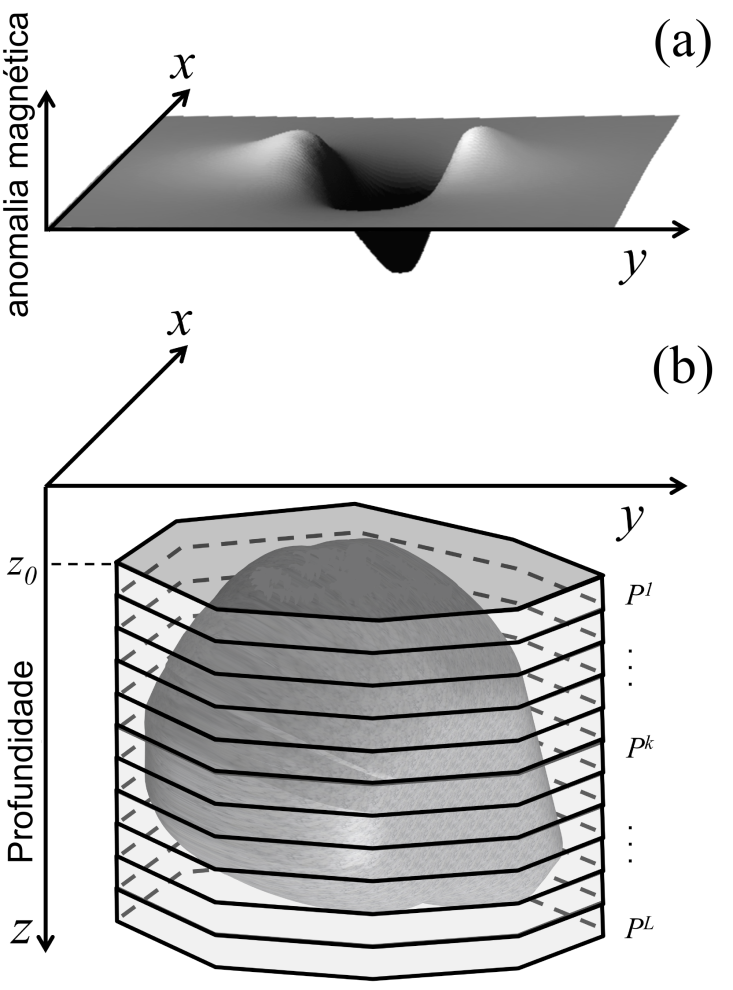
\includegraphics[scale=0.35]{schematic.png}
	\caption{Representação esquemática do modelo interpretativo. (a) Anomalia de campo total produzida por uma fonte magnética 3D localizada em subsuperfície (volume cinza escuro em b). (b) Modelo interpretativo formado por $ L $ prismas retos, verticalmente justapostos e com seção horizontal descrita por um polígono. A profundidade do topo $z_0$ do modelo interpretativo coincide com a da fonte magnética (volume cinza escuro).}
	\label{fig:schematic}
\end{figure}

%FIGURA
\begin{figure}[!htb]
	\centering
	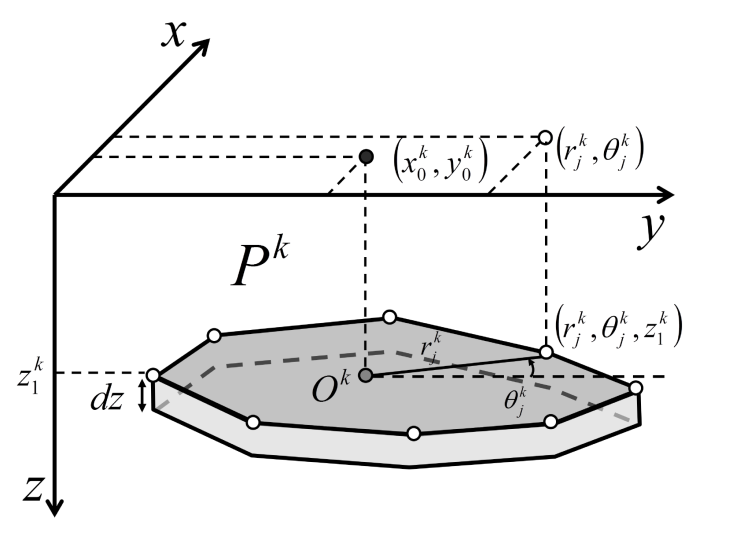
\includegraphics[scale=0.45]{pk.png}
	\caption{Representação esquemática do $k$-ésimo prisma $P^k$, $k=1,\dots, L$, que compõe o modelo interpretativo (Figura 1b). Este prisma tem espessura dz, profundidade do topo $z_1^k$ e seção horizontal descrita por um polígono com $V$ vértices igualmente espaçados entre $0^{\circ}$ e $360^{\circ}$.
}
	\label{fig:pk}
\end{figure}
\pagebreak

\section{Problema inverso}

Este trabalho propõe um método robusto de inversão magnética para estimar a posição e a forma de uma fonte magnética alvo 3D, que pode ou não estar na presença de fontes não-alvo.
O método foi formulado como um problema de otimização não-linear vinculado para estimar um vetor de parâmetros $\mathbf{p}$ (Equação \ref{eq:p-vector}) minimizando a função objetivo
\begin{equation}
\Gamma (\mathbf{p}) = \phi (\mathbf{p}) + \sum\limits^{5}_{\ell =1} \alpha_{\ell} \, \varphi_{\ell}(\mathbf{p}) \: ,
\label{eq:gamma}
\end{equation}
sujeito aos vínculos de desigualdade
\begin{equation}
p_{l}^{min} < p_{l} < p_{l}^{max}, \quad l = 1, \dots, M \: ,
\label{eq:inequality-constraints}
\end{equation}
em que $p_{l}^{min}$ e $p_{l}^{max}$ definem, respectivamente, os limites inferior e superior para o $l$-ésimo elemento $p_{l}$ do vetor de parâmetros $\mathbf{p}$,
$\varphi_{\ell}(\mathbf{p})$ são as funções que representam os vínculos que impõem informação a priori sobre a forma da estimativa do corpo 3D, e $\phi (\mathbf{p})$ 
é a função desajuste dos dados -- ou \textit{data-misfit} em inglês.
Podemos definir $\phi (\mathbf{p})$ através de duas abordagens diferentes com o propósito de comparar os resultados. Na primeira abordagem, $\phi (\mathbf{p})$ como
\begin{equation}\label{eq:L2_misfit}
\phi (\mathbf{p}) = \frac{1}{N} 
\| \mathbf{d}^{o} - \mathbf{d}(\mathbf{p}) \|_{2}^{2} \quad ,
\end{equation}
que é a norma-2 quadrática \citep[por exemplo,][p. 331]{aster_etal2019} dos resíduos entre o vetor de dados observados $\mathbf{d}^{o}$, cujo $i$-ésimo elemento $d_{i}^{o}$ representa a anomalia de campo total observada no ponto $(x_{i}, y_{i}, z_{i})$, e o vetor de dados preditos $\mathbf{d}(\mathbf{p})$, cujo $i$-ésimo elemento $d_{i} (\mathbf{p})$ é definido pela Equação \ref{eq:predicted-data-i}.
Alternativamente, podemos definir a função \textit{data-misfit} como
\begin{equation}\label{eq:L1_misfit}
\phi (\mathbf{p}) = \frac{1}{N} 
\| \mathbf{d}^{o} - \mathbf{d}(\mathbf{p}) \|_{1} \quad ,
\end{equation}
que representa a norma-1 \citep[por exemplo,][p. 331]{aster_etal2019}
dos resíduos entre os vetores de dados observados $\mathbf{d}^{o}$ e preditos $\mathbf{d}(\mathbf{p})$.
É de amplo conhecimento que o vetor de parâmetros que minimiza a norma-2 quadrática (Equação \ref{eq:L2_misfit}) pode ser muito afetado negativamente pela presença de \textit{outliers} e também pelo efeito causado por fontes não-alvo \cite[por exemplo,][]{claerbout_muir1973, 
	silva_hohmann1983, scales_gersztenkorn1988, silva_cutrim1989, farquharson_oldenburg1998, 
	uieda_barbosa2012, oliveirajr_etal2015, aster_etal2019}.
Através da estimativa do vetor de parâmetros obtida pela minimização da norma-1 (Equação \ref{eq:L1_misfit}), espera-se que a posição e a forma estimadas do corpo 3D durante a inversão ajustem a anomalia de campo total produzida pela fonte alvo e ignorem a causada pelas fontes não-alvo.

Na Equação \ref{eq:gamma}, $\alpha_{\ell}$, $\ell = 1, \dots, 5$, são escalares positivos que definem o peso relativo das funções dos vínculos $\varphi_{\ell}(\mathbf{p})$.
Essas funções são definidas seguindo a mesma abordagem utilizada por \citet{oliveirajr_etal2011} e \citet{oliveirajr_barbosa2013}.

\section{Vínculos}\label{sec:constraints}

As funções dos vínculos $\varphi_{\ell}(\mathbf{p})$ (Equação \ref{eq:gamma}), $\ell = 1, \dots, 5$, utilizadas aqui para obter soluções estáveis e introduzir informação a priori sobre o corpo estimado, foram organizadas em dois grupos para um melhor entendimento.

\subsection{Vínculos de suavidade}

Este grupo é formado pelas variações da regularização de Tikhonov de primeira ordem \cite[][ p. 103]{aster_etal2019} que impõe suavidade sobre os raios $r_{j}^{k}$ e sobre as coordenadas Cartesianas $x_{0}^{k}$ e $y_{0}^{k}$ da origem $O^{k}$, $j = 1, \dots, V$, $k = 1, \dots, L$, que define a seção horizontal de cada prisma (Fig.\ref{fig:schematic}b).
Elas foram propostas por \cite{oliveirajr_etal2011} e \cite{oliveirajr_barbosa2013} e possuem um papel muito importante em introduzir informação a priori sobre a forma da fonte alvo. 

O primeiro vínculo deste grupo é a \textit{suavidade sobre os raios adjacentes que definem a seção horizontal de cada prisma}. Esse vínculo impõe que os raios adjacentes $r_{j}^{k}$ e $r_{j+1}^{k}$ dentro do mesmo prisma devem ter comprimento semelhantes. Isso força que o prisma estimado terá uma forma aproximadamente cilíndrica, que evita descontinuidades abruptas entre as estimativas das distâncias radiais dentro de um mesmo prisma. Sua representação esquemática é mostrada na Figura \ref{fig:phi1}.

%FIGURA
\begin{figure}[!htb]
	\centering
	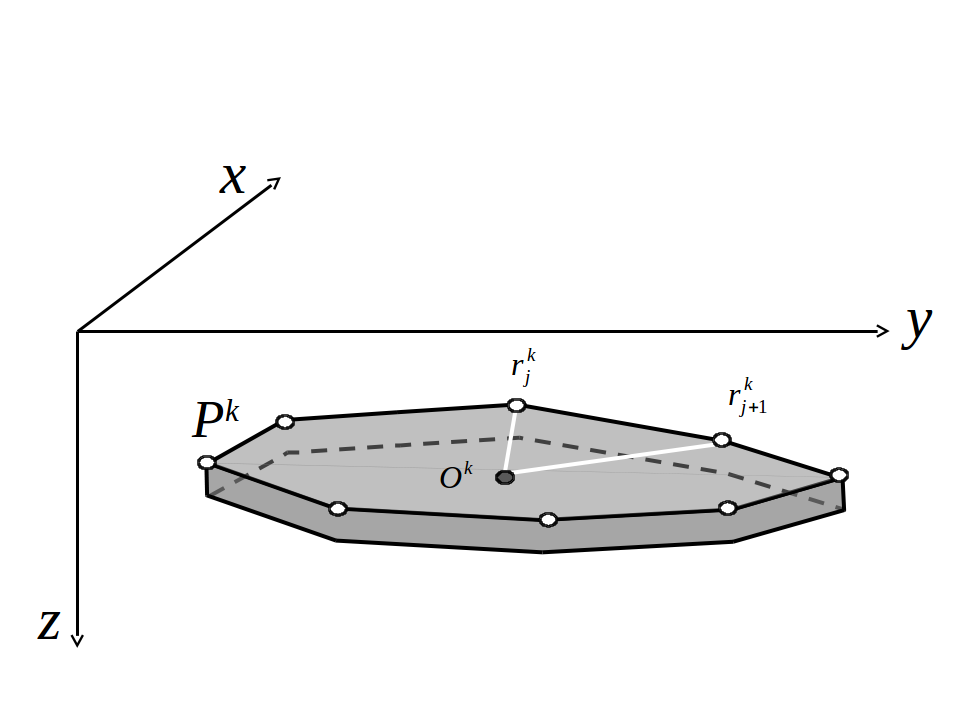
\includegraphics[scale=0.45]{Constraint_phi1.png}
	\caption{Representação esquemática do vínculo de suavidade sobre distâncias adjacentes dentro de um mesmo prisma $\varphi_{1}$. A figura exibe o k-ésimo prisma $P^k$ e as distâncias radiais adjacentes $r_j^k$ e $r_{j+1}^k$ relacionadas ao vínculo.}
	\label{fig:phi1}
\end{figure}

Matematicamente, o vínculo é dado por \begin{equation}\label{eq:phi1}
\begin{split}
\varphi_{1}(\mathbf{p}) &= \sum\limits^{L}_{k=1}\left[\left(r^{k}_{V}-r^{k}_{1}\right)^2 + \sum\limits^{V-1}_{j=1}\left(r^{k}_{j}-r^{k}_{j+1}\right)^2\right]\\
&= \mathbf{p}^{\mathsf{T}} \mathbf{R}^{\mathsf{T}}_{1}\mathbf{R}_{1} \mathbf{p} \quad ,
\end{split}
\end{equation}
em que
\begin{equation}
\mathbf{R}_{1} = 
\mathbf{I}_{L} \otimes 
\begin{bmatrix}
\left( \mathbf{I}_{V} - \mathbf{D}_{V}^\mathsf{T} \right) & \mathbf{0}_{V \times 2} \\
\end{bmatrix}_{LV \times M} \quad ,
\label{eq:S1-matrix}
\end{equation}
$\mathbf{I}_{L}$ é a matriz identidade de ordem $L$, ``$\otimes$" indica o produto de Kronecker \cite{}\cite[][ p. 243]{horn_johnson1991}, $\mathbf{0}_{V \times 2}$ é uma matriz de ordem $V \times 2$ com elementos nulos, 
$\mathbf{I}_{V}$ é a matriz identidade de ordem $V$ e $\mathbf{D}_{V}^\mathsf{T}$ é a matriz de permutação superior de ordem $V$ \cite[][ p. 20]{golub-vanloan2013}. O vetor gradiente e a matriz Hessiana da função $\varphi_{1}(\mathbf{p})$ (Equação \ref{eq:phi1}) são dados por:
\begin{equation}\label{eq:phi1_gh}
\begin{split}
\boldsymbol{\nabla}\varphi_{1}(\mathbf{p}) &= 2 \mathbf{R}^\mathsf{T}_{1}\mathbf{R}_{1}\mathbf{p} \quad , \\
\mathbf{H}_{1}(\mathbf{p}) &= 2\mathbf{R}^\mathsf{T}_{1}\mathbf{R}_{1} \quad .
\end{split}
\end{equation}

O segundo vínculo do grupo é a \textit{suavidade sobre os raios adjacentes de prismas adjacentes}, o qual impõe que os raios adjacentes $r_{j}^{k}$ e $r_{j}^{k+1}$ entre prismas verticalmente adjacentes tenham comprimentos semelhantes. Esse vínculo força que a forma de prismas verticalmente adjacentes seja similar. Uma representação esquemática do vínculo é apresentada na Figura \ref{fig:phi2}.

%FIGURA
\begin{figure}[!htb]
	\centering
	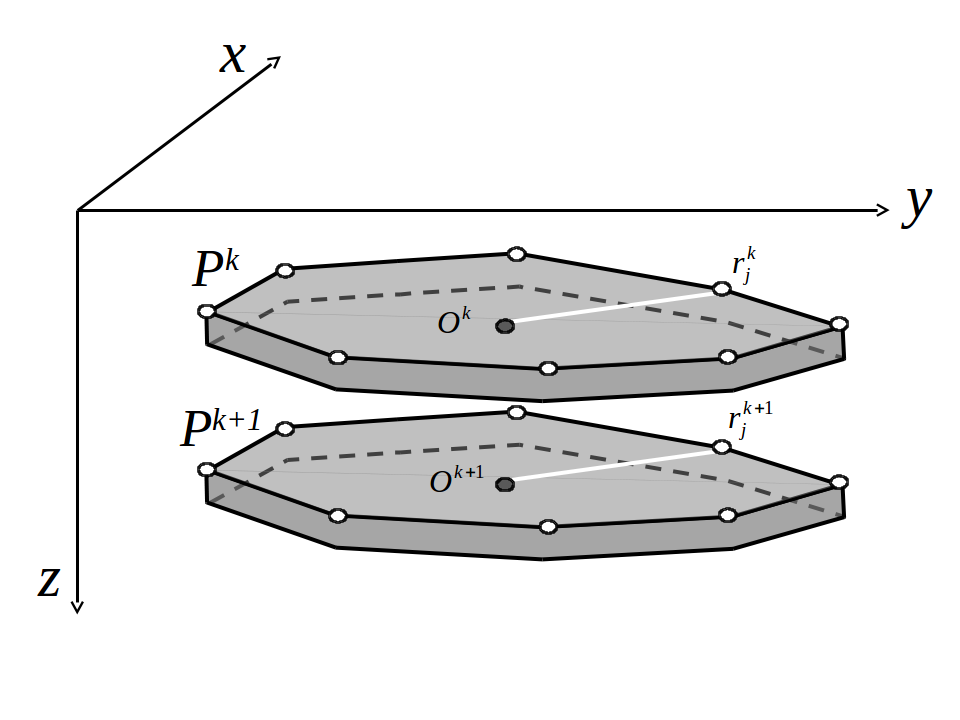
\includegraphics[scale=0.45]{Constraint_phi2.png}
	\caption{Representação esquemática do vínculo de suavidade sobre distâncias adjacentes pertencentes a prismas adjacentes $\varphi_{2}$. A figura exibe o k-ésimo prisma $P^k$ e seu adjacente $P^{k+1}$, assim como as distâncias radiais adjacentes $r_j^k$ e $r_j^{k+1}$ relacionadas ao vínculo.}
	\label{fig:phi2}
\end{figure}

De forma matemática o vínculo é dado por
\begin{equation}\label{eq:phi2}
\begin{split}
\varphi_{2}(\mathbf{p}) &= \sum\limits^{L-1}_{k=1}\left[\sum\limits^{V}_{j=1}\left(r^{k+1}_{j}-r^{k}_{j}\right)^2\right] \\
&= \mathbf{p}^{\mathsf{T}} \mathbf{R}^{\mathsf{T}}_{2}\mathbf{R}_{2}\mathbf{p}
\end{split} \quad ,
\end{equation}
em que
\begin{equation}
\mathbf{R}_{2} = 
\begin{bmatrix}
\mathbf{S}_{2} & \mathbf{0}_{(L-1)V \times 1} \\
\end{bmatrix}_{(L-1)V \times M} \quad ,
\label{eq:R2-matrix}
\end{equation}
\begin{equation}
\mathbf{S}_{2} =
\left( 
\begin{bmatrix} \mathbf{I}_{L-1} & \mathbf{0}_{(L-1) \times 1} \end{bmatrix} -
\begin{bmatrix} \mathbf{0}_{(L-1) \times 1} & \mathbf{I}_{L-1} \end{bmatrix} 
\right) \otimes 
\begin{bmatrix} \mathbf{I}_{V} & \mathbf{0}_{V \times 2} \end{bmatrix} \quad ,
\label{eq:S2-matrix}
\end{equation}
$\mathbf{0}_{(L-1)V \times 1}$ é um vetor de ordem $(L-1)V \times 1$ com elementos nulos,
$\mathbf{0}_{(L-1) \times 1}$ é um vetor de ordem $(L-1) \times 1$ com elementos nulos e 
$\mathbf{I}_{L-1}$ é a matriz identidade de ordem $L-1$. O vetor gradiente e a matriz Hessiana da função $\varphi_{2}(\mathbf{p})$ (Equação \ref{eq:phi2}) são dados por:
\begin{equation}\label{eq:phi2_gh}
\begin{split}
\boldsymbol{\nabla}\varphi_{2}(\mathbf{p}) &= 2\mathbf{R}^\mathsf{T}_{2}\mathbf{R}_{2}\mathbf{p} \quad ,\\
\mathbf{H}_{2}(\mathbf{p}) &= 2\mathbf{R}^\mathsf{T}_{2}\mathbf{R}_{2} \quad .
\end{split}
\end{equation}

O último vínculo deste grupo é a \textit{suavidade sobre a posição horizontal das origens arbitrárias de prismas verticalmente adjacentes}. Esse vínculo impõe que as coordenadas Cartesianas horizontais estimadas $(x_{0}^{k}, y_{0}^{k})$ e $(x_{0}^{k+1}, y_{0}^{k+1})$ das origens $O^{k}$ e $O^{k+1}$ 
de prismas verticalmente adjacentes devem ser próximas entre si. Isso controla o mergulho do corpo estimado através da regularização do deslocamento horizontal de prismas verticalmente adjacentes (Figura \ref{fig:phi3}).

%FIGURA
\begin{figure}[!htb]
	\centering
	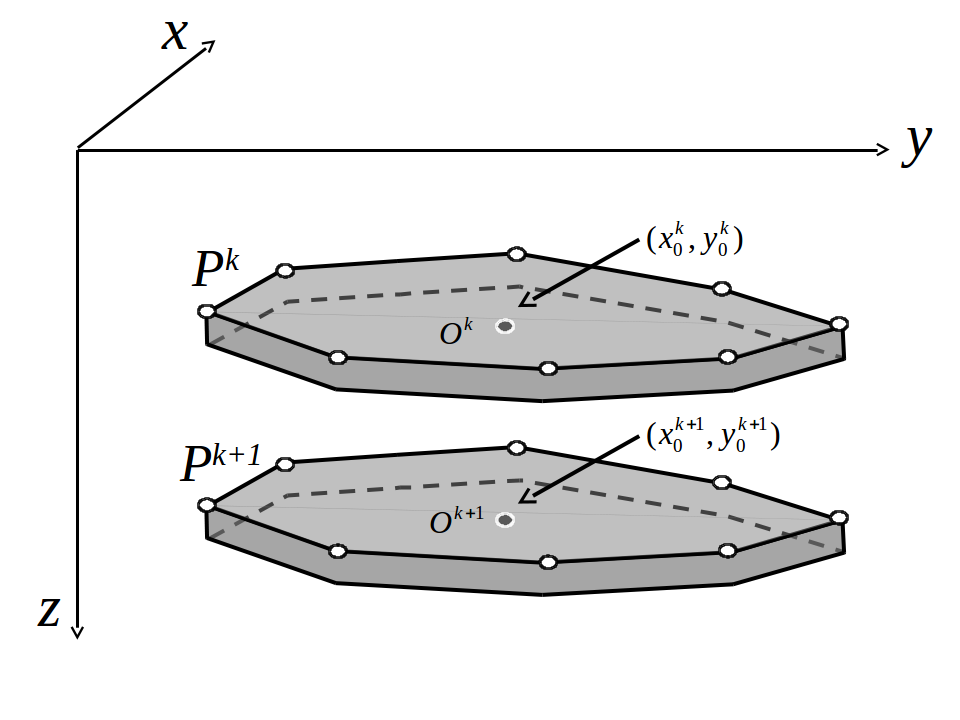
\includegraphics[scale=0.45]{Constraint_phi5.png}
	\caption{Representação esquemática do vínculo de suavidade nas coordenadas das origens pertencentes a prismas adjacentes $\varphi_{3}$. A figura exibe os prismas $P^k$ e $P^{k+1}$ e suas respectivas as coordenadas Cartesianas $(x_0^k,y_0^k)$, referidas à origem $O^k$, e $(x_0^{k+1},y_0^{k+1})$, referidas à origem $O^{k+1}$.}
	\label{fig:phi3}
\end{figure}

Algebricamente o vínculo é dado por
\begin{equation}\label{eq:phi3}
\begin{split}
\varphi_{3}(\mathbf{p}) &= \sum\limits^{L-1}_{k=1}\left[\left(x_{0}^{k+1} - x_{0}^{k}\right)^2 + \left(y_{0}^{k+1} - y_{0}^{k}\right)^2 \right] \\
&= \mathbf{p}^{\mathsf{T}} \mathbf{R}^{\mathsf{T}}_{3}\mathbf{R}_{3}\mathbf{p}
\end{split} \quad ,
\end{equation}
em que 
\begin{equation}
\mathbf{R}_{3} = 
\begin{bmatrix}
\mathbf{S}_{3} & \mathbf{0}_{(L-1)2 \times 1} \\
\end{bmatrix}_{(L-1)2 \times M} \quad ,
\label{eq:R3-matrix}
\end{equation}
\begin{equation}
\mathbf{S}_{3} =
\left( 
\begin{bmatrix} \mathbf{I}_{L-1} & \mathbf{0}_{(L-1) \times 1} \end{bmatrix} -
\begin{bmatrix} \mathbf{0}_{(L-1) \times 1} & \mathbf{I}_{L-1} \end{bmatrix} 
\right) \otimes 
\begin{bmatrix} \mathbf{0}_{2 \times V} & \mathbf{I}_{2} \end{bmatrix} \quad ,
\label{eq:S3-matrix}
\end{equation}
$\mathbf{0}_{(L-1)2 \times 1}$ é um vetor de ordem $(L-1)2 \times 1$ com elementos nulos,
$\mathbf{0}_{2 \times V}$ é uma matrix de ordem $2 \times V$ com elementos nulos e 
$\mathbf{I}_{2}$ é uma matriz identidade de ordem $2$. O vetor gradiente e a matriz Hessiana da função $\varphi_{3}(\mathbf{p})$ (Equação \ref{eq:phi3}) são dados por:
\begin{equation}\label{eq:phi3_gh}
\begin{split}
\boldsymbol{\nabla}\varphi_{3}(\mathbf{p}) &= 2\mathbf{R}^\mathsf{T}_{3}\mathbf{R}_{3}\mathbf{p} \quad ,\\
\mathbf{H}_{3}(\mathbf{p}) &= 2\mathbf{R}^\mathsf{T}_{3}\mathbf{R}_{3} \quad .
\end{split}
\end{equation}

\subsection{Vínculos de norma Euclidiana mínima}

Dois vínculos utilizam a regularização Tikhonov de ordem zero com o propósito de estabilizar de maneira puramente matemática o problema inverso sem necessariamente introduzir informação a priori com significado físico sobre a fonte. 

A \textit{norma Euclidiana mínima dos raios} impões que todos os raios estimados dentro de um prisma devem ser próximos de zero (Figura \ref{fig:phi4}).

%FIGURA
\begin{figure}[!htb]
	\centering
	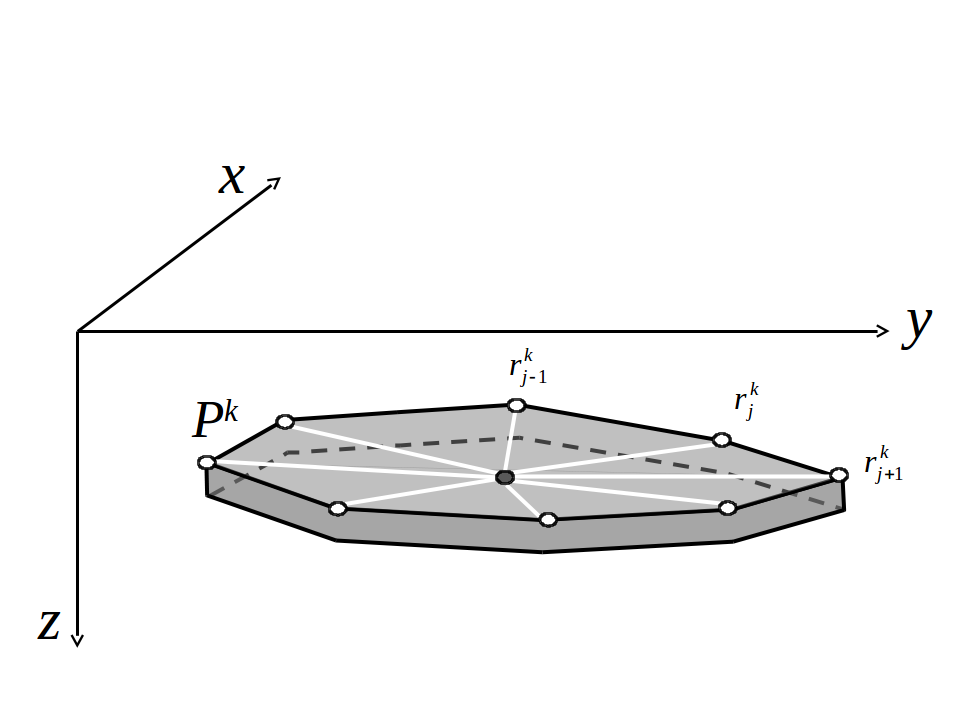
\includegraphics[scale=0.45]{Constraint_phi6.png}
	\caption{Representação esquemática do vínculo de Tikhonov de ordem zero nas distâncias radiais de um prisma $\varphi_{4}$. A figura exibe os prisma $P^k$ e suas respectivas distâncias radiais $r_j^k$ referidas à origem $O^k$. O vínculo atua sobre as distâncias radiais do prismas, levando-as próximas a zero.}
	\label{fig:phi4}
\end{figure}

Esse vínculo foi proposto por \cite{oliveirajr_etal2011} e \cite{oliveirajr_barbosa2013} e pode ser reescrito como
\begin{equation}\label{eq:phi4}
\begin{split}
\varphi_{4}(\mathbf{p}) &= \sum\limits^{L}_{k=1}\sum\limits^{V}_{j=1}\left(r_{j}^{k}\right)^2 \\
&= \mathbf{p}^{\mathsf{T}} \mathbf{R}_{4}^{\mathsf{T}} \mathbf{R}_{4} \mathbf{p}
\end{split} \quad ,
\end{equation}
em que
\begin{equation}
\mathbf{R}_{4} = 
\begin{bmatrix}
\mathbf{S}_{4} & \mathbf{0}_{(M-1) \times 1} \\
\mathbf{0}_{1 \times (M-1)} & 0 \\
\end{bmatrix}_{M\times M} \quad ,
\label{eq:R4-matrix}
\end{equation}
e
\begin{equation}
\mathbf{S}_{4} = 
\begin{bmatrix}
\mathbf{I}_{V} & \mathbf{0}_{V \times 2} \\
\mathbf{0}_{2 \times V} & \mathbf{I}_{2} \\
\end{bmatrix}_{ (V+2)\times (V+2)} \quad .
\label{eq:S4-matrix}
\end{equation}
O vetor gradiente e a matriz Hessiana da função $\varphi_{4}(\mathbf{p})$ (Equação \ref{eq:phi4}) são:
\begin{equation}\label{eq:phi4_gh}
\begin{split}
\boldsymbol{\nabla}\varphi_{4}(\mathbf{p}) &= 2\mathbf{R}^\mathsf{T}_{4}\mathbf{R}_{4}\mathbf{p} \quad ,\\
\mathbf{H}_{4}(\mathbf{p}) &= 2\mathbf{R}^\mathsf{T}_{4}\mathbf{R}_{4} \quad .
\end{split}
\end{equation}

Finalmente, o último vínculo é a \textit{norma Euclidiana mínima da espessura}, que impõe que a espessura comum $ dz $ de todos os prismas seja próxima de zero. Esse vínculo força que a profundidade da base do modelo seja o mais rasa possível (Figura \ref{fig:phi5})

%FIGURA
\begin{figure}[!htb]
	\centering
	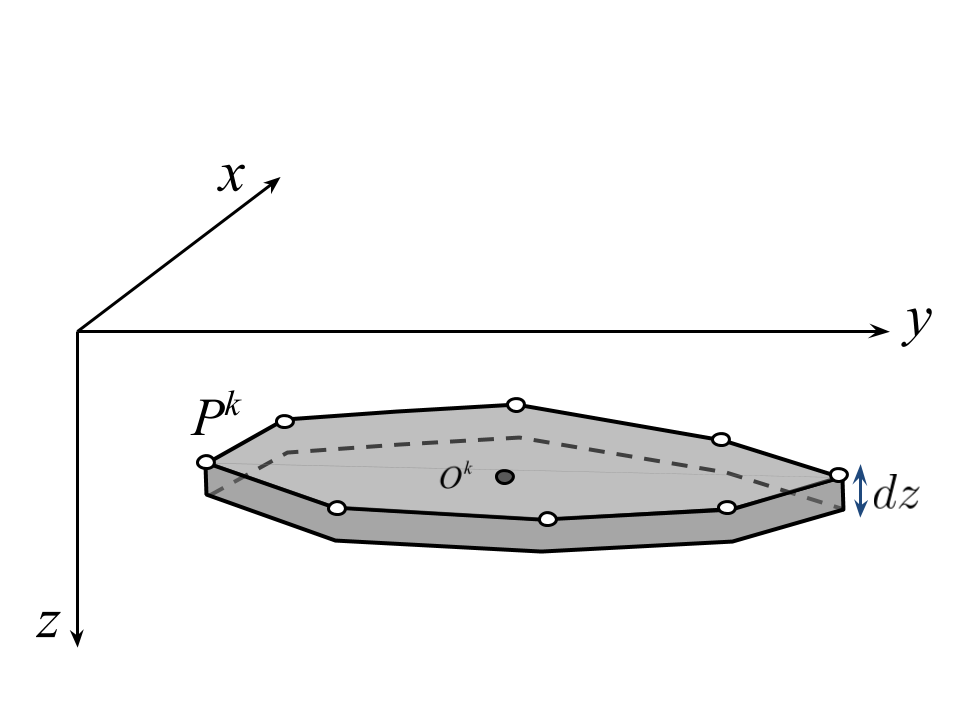
\includegraphics[scale=0.35]{Constraint_phi7.png}
	\caption{Representação esquemática do vínculo de Tikhonov de ordem zero $\varphi_{5}$ na espessura $dz$ dos prismas. A figura exibe os prisma $P^k$ e sua espessura. O vínculo atua sobre a espessura de os todos prismas levando-a próxima a zero, uma vez que $dz$ é igual para todos os prismas.}
	\label{fig:phi5}
\end{figure}

Esse vínculo pode ser escrito matematicamente como
\begin{equation}\label{eq:phi5}
\begin{split}
\varphi_{5}(\mathbf{p}) &= dz^2 \\
&= \mathbf{p}^{\mathsf{T}} \mathbf{R}_{5}^{\mathsf{T}} \mathbf{R}_{5} \mathbf{p}
\end{split} \quad ,
\end{equation}
em que
\begin{equation}
\mathbf{R}_{5} =
\begin{bmatrix}
\mathbf{0}_{(M-1) \times (M-1)} & \mathbf{0}_{(M-1) \times 1} \\
\mathbf{0}_{1 \times (M-1)} & 1 \\
\end{bmatrix}_{ M \times M } \quad .
\end{equation}
O vetor gradiente e a matriz Hessiana da função $\varphi_{5}(\mathbf{p})$ (Equação \ref{eq:phi5}) são:
\begin{equation}\label{eq:phi5_gh}
\begin{split}
\boldsymbol{\nabla}\varphi_{5}(\mathbf{p}) &= 2\mathbf{R}^\mathsf{T}_{5}\mathbf{R}_{5}\mathbf{p} \quad ,\\
\mathbf{H}_{5}(\mathbf{p}) &= 2\mathbf{R}^\mathsf{T}_{5}\mathbf{R}_{5} \quad .
\end{split}
\end{equation}

\section{Algoritmo de inversão}

Dada uma profundidade do topo do prisma mais raso $z_{0}$, a intensidade de magnetização total $m_{0}$ de todos os prismas, uma aproximação inicial $\hat{\mathbf{p}}_{(0)}$ para o vetor de parâmetros $\mathbf{p}$ (Equação \ref{eq:p-vector}), e os limites 
$p_{l}^{min}$ e $p_{l}^{max}$ (Equação \ref{eq:inequality-constraints}), o método de Levenberg-Marquardt \cite[por exemplo, ][ p. 624]{seber_wild2003} é utilizado para estimar o vetor de parâmetros $\hat{\mathbf{p}}^{\ast}$ que minimiza a função objetivo $\Gamma (\mathbf{p})$ (Equação \ref{eq:gamma}), sujeita aos vínculos de desigualdade definidos pela Equação \ref{eq:inequality-constraints}.
Para incorporar esses vínculos de desigualdade, foi empregada a mesma abordagem apresentada por \cite{barbosa_etal1999}, \cite{oliveirajr_etal2011} e \cite{oliveirajr_barbosa2013}.
Abaixo, segue o algoritmo de inversão aqui proposto:

\begin{itemize}
	\item[\textbf{entrada}] $\mathbf{d}^{o}$, $D_{0}$, $I_{0}$, $z_{0}$, 
	$m_{0}$, $D$, $I$, $p_{l}^{min}$ e $p_{l}^{max}$ (Equação 
	\ref{eq:inequality-constraints}), $k = 0$, $\hat{\mathbf{p}}_{(k)}$, e
	$\mathbf{W}_{(k)} = \mathbf{I}$, em que $\mathbf{I}$ é a matriz identidade de ordem $M$.
	\item[\textbf{(1)}] Computa a matriz $N \times M$ $\mathbf{G}(\hat{\mathbf{p}}_{(k)})$, cujo elemento $ij$ é a derivada do dado $d_{i}(\hat{\mathbf{p}}_{(k)})$ 
	(Equação \ref{eq:predicted-data-i}) com respeito ao $j$-ésimo elemento $p_{j}$ do vetor de parâme\-tros $\mathbf{p}$ (Equação \ref{eq:p-vector}):
	$$
	g_{ij} =  \dfrac{\partial d_{i}(\hat{\mathbf{p}}_{(k)})}{\partial{p_j}} \: .
	$$
	\item[\textbf{(2)}] Computa o vetor gradiente 
	$$
	\boldsymbol{\nabla} \phi(\hat{\mathbf{p}}_{(k)}) = 
	- \frac{2}{N} \mathbf{G}(\hat{\mathbf{p}}_{(k)})^{\top} 
	\mathbf{W}_{(k)} 
	\left[ \mathbf{d}^{o} - \mathbf{d}(\hat{\mathbf{p}}_{(k)}) \right]
	$$
	e a matriz Hessiana
	$$
	\mathbf{H}_{\phi}(\hat{\mathbf{p}}_{(k)}) = \frac{2}{N} 
	\mathbf{G}(\hat{\mathbf{p}}_{(k)})^{\top} \mathbf{W}_{(k)} 
	\mathbf{G}(\hat{\mathbf{p}}_{(k)})
	$$
	da função \textit{data-misfit} $\phi (\mathbf{p})$ (Equação \ref{eq:L2_misfit}),
	quando $\mathbf{W}_{(k)} = \mathbf{I}$, ou $\phi (\mathbf{p})$ 
	(Equação \ref{eq:L1_misfit}), quando $\mathbf{W}_{(k)} \ne \mathbf{I}$.
	Na próxima seção, será discutido como usar a matriz Hessiana 
	$\mathbf{H}_{\phi}(\hat{\mathbf{p}}_{(0)})$ (computada na iteração $k = 0$) 
	para definir os pesos $\alpha_{\ell}$ (Equação \ref{eq:gamma}) das funções de vínculos $\varphi_{\ell}(\mathbf{p})$ 
	(Equações \ref{eq:phi1}, \ref{eq:phi2}, \ref{eq:phi3}, \ref{eq:phi4} e \ref{eq:phi5}).
	\item[\textbf{(3)}] Computa o vetor gradiente 
	$$
	\boldsymbol{\nabla}\Gamma(\hat{\mathbf{p}}_{(k)}) = 
	\boldsymbol{\nabla}\phi (\hat{\mathbf{p}}_{(k)}) + 
	\sum\limits^{5}_{\ell =1} \alpha_{\ell} \, \boldsymbol{\nabla}\varphi_{\ell}(\hat{\mathbf{p}}_{(k)}) 
	$$ 
	e a matriz Hessiana
	$$
	\mathbf{H}(\hat{\mathbf{p}}_{(k)}) = 
	\mathbf{H}_\phi (\hat{\mathbf{p}}_{(k)}) + \sum\limits^{5}_{\ell =1} \alpha_{\ell} 
	\, \mathbf{H}_{\ell}
	$$ 
	da função objetivo $\Gamma (\mathbf{p})$ (Equação \ref{eq:gamma}),
	em que $\boldsymbol{\nabla}\varphi_{\ell}(\hat{\mathbf{p}}_{(k)})$ e
	$\mathbf{H}_{\ell}$ são, respectivamente, o vetor gradiente e a matriz Hessiana (Equações \ref{eq:phi1_gh}, \ref{eq:phi2_gh}, \ref{eq:phi3_gh}, \ref{eq:phi4_gh} e \ref{eq:phi5_gh}) das funções dos vínculos $\varphi_{\ell}(\mathbf{p})$ (Equações \ref{eq:phi1}, \ref{eq:phi2}, \ref{eq:phi3}, \ref{eq:phi4} e \ref{eq:phi5}).	
	\item[\textbf{(4)}] Computa o $l$-ésimo elemento $\hat{p}^{\dagger}_{l}$ de um vetor $\hat{\mathbf{p}}^{\dagger}_{(k)}$ como:
	$$
	\hat{p}^{\dagger}_{l} = -\ln\left(\frac{p_{l}^{max} - \hat{p}_{l}}{\hat{p}_{l} - p_{l}^{min}}\right) \: ,
	$$
	em que $\hat{p}_{l}$ é o $l$-ésimo elemento de $\hat{\mathbf{p}}_{(k)}$.
	\item[\textbf{(5)}] Computa uma matriz diagonal $\mathbf{T}(\hat{\mathbf{p}}_{(k)})$ 
	com o elemento $t_{ll}$ dado por
	$$
	t_{ll}(\hat{p}_{l}) = \frac{(p_{l}^{max} - \hat{p}_{l})(\hat{p}_{l} - p_{l}^{min})}{p_{l}^{max} - p_{l}^{min}} \: ,
	$$
	em que $p_{l}$ é o $l$-ésimo elemento do vetor $\hat{\mathbf{p}}_{(k)}$.
	\item[\textbf{(6)}] Computa uma matriz 
	$$
	\mathbf{H}^{\dagger}(\hat{\mathbf{p}}_{(k)}) = \mathbf{H}(\hat{\mathbf{p}}_{(k)})\mathbf{T}(\hat{\mathbf{p}}_{(k)}) \: .
	$$
	\item[\textbf{(7)}] Computa uma matriz diagonal $\mathbf{Q}_{(k)}$ com elemento $q_{ll}$ dado por 
	$$
	q_{ll} = \frac{1}{\sqrt{h^{\dagger}_{ll}}} \: ,
	$$
	em que $h^{\dagger}_{ll}$ é o elemento $ll$ da matriz $\mathbf{H}^{\dagger}(\hat{\mathbf{p}}_{(k)})$ .
	\item[\textbf{(8)}] Computa uma correção 
	$\boldsymbol{\Delta}\hat{\mathbf{p}}^{\dagger}_{(k)}$ para o vetor 
	$\hat{\mathbf{p}}^{\dagger}_{(k)}$ pela solução do sistema linear
	$$
	\mathbf{Q}_{(k)}^{-1} \left[ \mathbf{Q}_{(k)} 
	\mathbf{H}^{\dagger}(\hat{\mathbf{p}}_{(k)}) \mathbf{Q}_{(k)} + 
	\lambda_{(k)} \mathbf{I}_{M} \right] \mathbf{Q}_{(k)}^{-1}
	\boldsymbol{\Delta} \hat{\mathbf{p}}^{\dagger}_{(k)} = 
	- \boldsymbol{\nabla}\Gamma(\hat{\mathbf{p}}_{(k)}) \: ,
	$$
	%	$$
	%	\left[ \mathbf{H}^{\dagger}(\hat{\mathbf{p}}_{(k)}) + 
	%	\lambda_{(k)} \mathbf{D}_{(k)} \right] \boldsymbol{\Delta} \hat{\mathbf{p}}^{\dagger}_{(k)} = 
	%	- \boldsymbol{\nabla}\Gamma(\hat{\mathbf{p}}_{(k)}) \: ,
	%	$$
	em que $\lambda_{(k)}$ é um escalar positivo ajustado à cada iteração
	%	and $\mathbf{D}_{(k)}$ is a diagonal matrix formed by the diagonal elements 
	%	of $\mathbf{H}^{\dagger}(\hat{\mathbf{p}}_{(k)})$
	\citep[por exemplo,][p. 624]{seber_wild2003}.
	\item[\textbf{(9)}] Computa um novo vetor 
	%	\item[\textbf{(8)}] Compute a new vector 
	$$
	\hat{\mathbf{p}}^{\dagger}_{(k+1)} = \hat{\mathbf{p}}^{\dagger}_{(k)} + \boldsymbol{\Delta}\hat{\mathbf{p}}^{\dagger}_{(k)} \: .
	$$
	\item[\textbf{(10)}] Computa o $l$-ésimo elemento $ \hat{p}_{l} $ do novo vetor
	%	\item[\textbf{(9)}] Compute the $l$th element of the new vector 
	$\hat{\mathbf{p}}_{(k+1)}$ como:
	$$
	\hat{p}_{l} = p_{l}^{min} + \left(\frac{p_{l}^{max} - p_{l}^{min}}{ 1 + e^{-\hat{p}^{\dagger}_{l}} }\right) \: .
	$$
	\item[\textbf{(11)}] Se o seguinte critério de convergência for satisfeito,
	%	\item[\textbf{(10)}] If the following convergence criterion is satisfied,
	$$
	\Bigg|
	\frac{\Gamma(\hat{\mathbf{p}}_{(k+1)}) - \Gamma(\hat{\mathbf{p}}_{(k)})}
	{\Gamma(\hat{\mathbf{p}}_{(k)})} 
	\Bigg| \le \tau \: ,
	$$ 
	em que $\tau$ é um número positivo pequeno, que varia de $\approx 10^{-3}$ a 
	$10^{-4}$, que controla a convergência, o vetor de parâmetros $\hat{\mathbf{p}}_{(k+1)}$ é a solução. 
	Senão, atualiza o vetor de parâmetros 
	$$
	\hat{\mathbf{p}}_{(k)} \leftarrow \hat{\mathbf{p}}_{(k+1)} \: ,
	$$
	atualiza o elemento $ii$ da matriz $\mathbf{W}_{(k)}$
	$$
	w_{ii} = \frac{1}{\mid d_{i}^{o} -d_{i}(\hat{\mathbf{p}}_{(k)}) \mid + 
		\, \varepsilon} \: ,
	$$
	em que $\varepsilon$ possui um valor positivo pequeno ($\approx 10^{-10}$) usado
	para prevenir uma divisão por zero, atualiza o contador da iteração $k$
	$$
	k \leftarrow k + 1 \: ,
	$$
	e retorna à etapa (1).
\end{itemize}

Neste algoritmo, os elementos da matriz $\mathbf{G}(\hat{\mathbf{p}}_{(k)})$ 
(etapa 1) são computados pelo uso das diferenças finitas centradas.
É importante notar que na etapa 3 as matrizes Hessianas $\mathbf{H}_{\ell}$ (Equações \ref{eq:phi1_gh}, \ref{eq:phi2_gh}, \ref{eq:phi3_gh}, \ref{eq:phi4_gh} e \ref{eq:phi5_gh})
das funções dos vínculos $\varphi_{\ell}(\mathbf{p})$ 
(Equações \ref{eq:phi1}, \ref{eq:phi2}, \ref{eq:phi3}, \ref{eq:phi4} e \ref{eq:phi5}) 
não dependem do vetor de parâmetros. Por essa razão, eles são computados apenas uma vez antes da primeira iteração e armazenados para serem usados até a convergência ser alcançada (etapa 11).

Este algoritmo é executado para obter um corpo estimado para cada ponto 
$(m_{0}, z_{0})$ em uma malha de valores de profundidade do topo $z_{0}$ e intensidade de magnetização total $m_{0}$ definida pelo usuário. 
Todos os corpos estimados são obtidos através da utilização de uma aproximação inicial $\hat{\mathbf{p}}_{(0)}$ para o vetor de parâmetros
$\mathbf{p}$ (Equação \ref{eq:p-vector}), dos mesmos valores para os pesos
$\alpha_{\ell}$ (Equação \ref{eq:gamma}) e dos limites $p_{l}^{min}$ e 
$p_{l}^{max}$ (Eq. \ref{eq:inequality-constraints}) para os parâmetros estimados.
Os valores ótimos da profundidade do topo $z_{0}$ e intensidade de magnetização total
$m_{0}$ são escolhidos como aqueles associados aos corpos estimados que produzem os menores valores da função objetivo $\Gamma (\mathbf{p})$ (Equação \ref{eq:gamma}).

Note que, ao manter a matriz $\mathbf{W}_{(k)}$ (etapa 2 e 10) igual à identidade ao longo das iterações, o corpo estimado minimiza a norma-2 quadrática dos resíduos entro os dados observados e preditos (Equação \ref{eq:L2_misfit}). 
Nesse caso, o corpo estimado é a solução L2. 
A atualização iterativa dos elementos da matriz $\mathbf{W}_{(k)}$ com os valores absolutos dos resíduos de acordo com a etapa 10 é feita através do método IRLS \citep[][p. 46]{scales_gersztenkorn1988, aster_etal2019} para obter um corpo estimado que minimiza a norma-1 dos resíduos entre os dados observados e preditos 
(Equação \ref{eq:L1_misfit}). Nesse caso, o corpo estimado é a solução L1.

\section{Considerações práticas}

Nesta seção serão apresentados alguns aspectos práticos de como definir o conjunto de valores de profundidade do topo do prisma mais raso $z_{0}$, a intensidade de magnetização total $m_{0}$, a aproximação inicial
$\hat{\mathbf{p}}_{(0)}$ para o vetor de parâmetros $\mathbf{p}$ (Equação \ref{eq:p-vector}),
os pesos $\alpha_{\ell}$ (Equação \ref{eq:gamma}) das funções de vínculos 
$\varphi_{\ell}(\mathbf{p})$ 
(Equações \ref{eq:phi1}, \ref{eq:phi2}, \ref{eq:phi3}, \ref{eq:phi4} e \ref{eq:phi5}) e os limites $p_{l}^{min}$ e $p_{l}^{max}$ dos vínculos de desigualdade (Equação 
\ref{eq:inequality-constraints}).

Inicialmente, calcula-se a redução ao polo da anomalia de campo total observada. Essa é uma etapa dupla: ele permite a verificação dos valores usados para a direção de magnetização total (declinação $D$ e inclinação $I$) e é utilizado para estimar as dimensões horizontais da fonte alvo.
Se a fonte alvo possui uma direção de magnetização uniforme com valores de declinação e inclinação próximos daqueles escolhidos para $D$ e $I$, a anomalia RTP é predominantemente positiva sobre a fonte alvo e decai a zero perto de seus limites laterais.
Através da anomalia RTP estimada pela camada equivalente, é possível definir os limites $p_{l}^{min}$ e $p_{l}^{max}$ (Figura \ref{fig:barreira}) dos vínculos de desigualdade (Equação \ref{eq:inequality-constraints}) e uma aproximação inicial cilíndrica $\hat{\mathbf{p}}_{(0)}$, isto é, todos os prismas que formam $\hat{\mathbf{p}}_{(0)}$ possuem os vértices definidos por uma mesma distância radial constante $r_{0}$ e a mesma origem $(x_{0}, y_{0})$.
Nesta etapa, os pesos são $\alpha_{\ell}$ (Equação \ref{eq:gamma}) estabelecidos iguais a zero e se define uma malha de valores para a profundidade do topo $z_{0}$, intensidade de magnetização total $m_{0}$ e espessura $dz$ que produz, sem grande rigor, um ajuste entre dados observados $\mathbf{d}^{o}$ e dados preditos $\mathbf{d}(\hat{\mathbf{p}}_{(0)})$.

\pagebreak

%FIGURA
\begin{figure}[!htb]
	\centering
	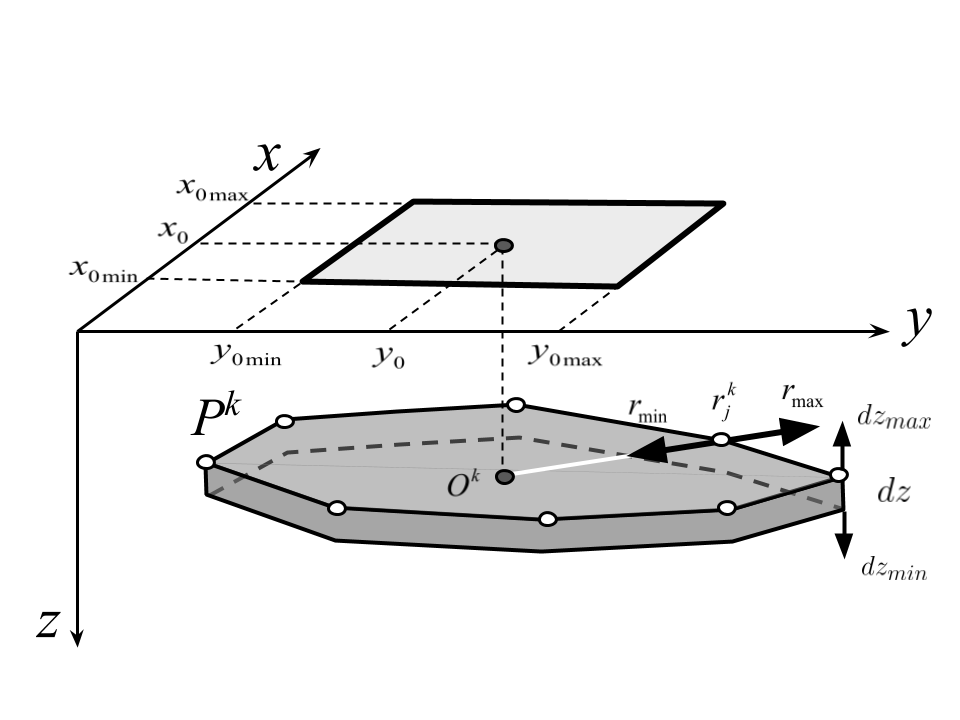
\includegraphics[width=0.75\linewidth]{Constraint_barrier.png}
	\caption{Representação esquemática dos vínculos de desigualdade. A figura exibe os prisma $P^k$ e os intervalos de máximo e mínimo de $r^k_j$, $x_0$, $y_0$ e $ dz $.}
	\label{fig:barreira}
\end{figure}

Um segundo aspecto crucial desse algoritmo consiste em definir os valores dos pesos $\alpha_{\ell}$ (Equação \ref{eq:gamma}). 
Não existe uma regra analítica para defini-los e seus valores podem depender das particularidades da área de estudo e do conjunto de dados observados.
Para contornar esse problema, os pesos $\alpha_{\ell}$ são definidos da seguinte maneira:
\begin{equation}\label{eq:alphas}
\alpha_{\ell} = \tilde{\alpha}_{\ell} \frac{E_{\phi}}{E_{\ell}}, 
\quad \ell = 1,\dots, 5 \: ,
\end{equation}
em que $\tilde{\alpha}_{\ell}$ é um escalar positivo e $ E_{\phi}/E_{\ell} $ 
é o fator de normalização.
Nessa equação, $E_{\ell}$ representa o traço da matriz Hessiana $\mathbf{H}_{\ell}$ (Equações \ref{eq:phi1_gh}, \ref{eq:phi2_gh}, \ref{eq:phi3_gh}, \ref{eq:phi4_gh} e \ref{eq:phi5_gh}) da $\ell$-ésima função de vínculo $\varphi_{\ell}(\mathbf{p})$
(Equações \ref{eq:phi1}, \ref{eq:phi2}, \ref{eq:phi3}, \ref{eq:phi4} e \ref{eq:phi5}).
A constante $E_{\phi}$ é o traço da matriz Hessiana
$\mathbf{H}_{\phi}(\hat{\mathbf{p}}_{(0)})$ (etapa 2 do algoritmo) da função \textit{data-misfit} $\phi(\mathbf{p})$ (Equação \ref{eq:L1_misfit}) computada na iteração
$k = 0$, com a aproximação inicial $\hat{\mathbf{p}}_{(0)}$ para o vetor de parâmetros $ \mathbf{p} $ (Equação \ref{eq:p-vector}).
Essa estratégia empírica permite definir indiretamente os pesos $\alpha_{\ell}$ 
(Equação \ref{eq:gamma}) pela utilização dos pesos normalizados $\tilde{\alpha}_{\ell}$ 
(Equação \ref{eq:alphas}), os quais dependem menos das características particulares do problema.
Baseado em experiência prática, os valores iniciais propostos aqui para os pesos normalizados $\tilde{\alpha}_{\ell}$ para ambas as funções \textit{data-misfit}, definidas pelas Equações \ref{eq:L2_misfit} e \ref{eq:L1_misfit}, são:
$\tilde{\alpha}_{1} = 10^{-4}$, $\tilde{\alpha}_{2} = 10^{-4}$, 
$\tilde{\alpha}_{3} = 10^{-4}$, $\tilde{\alpha}_{4} = 10^{-7}$, e 
$\tilde{\alpha}_{5} = 10^{-5}$.
Esses valores são comumente refinados de acordo com a informação a priori sobre a complexidade da fonte alvo. Por exemplo, ao aumentar ou diminuir valor de $\tilde{\alpha}_{1}$, força-se que o corpo estimado tenha fatias horizontais mais ou menos suaves; ao aumentar ou diminuir o valor de $\tilde{\alpha}_{3}$, força-se que o corpo estimado seja mais ou menos vertical. Os pesos normalizados
$\tilde{\alpha}_{1}$, $\tilde{\alpha}_{2}$, e $\tilde{\alpha}_{3}$ são comumente usados para introduzir informação a priori sobre o formato da fonte alvo. O peso normalizado $\tilde{\alpha}_{4}$ é geralmente usado como um parâmetro de regularização puramente matemático para obter soluções estáveis. Finalmente, o peso normalizado $\tilde{\alpha}_{5}$ é usualmente escolhido com o propósito de obter um corpo estimado com a profundidade da base mais rasa o possível.
  \chapter{Procedimentos computacionais}

Os procedimentos computacionais pré-inversão deste método têm como propósito definir: (1) a aproximação inicial $ \hat{\mathbf{p}}_{(0)} $, (2) os limites superiores $ p_l^{max} $ e inferiores $ p_l^{min} $, $ l=1, \dots, M $, do vínculo de desigualdade (Eq. \ref{eq:inequality-constraints}) e (3) os pesos normalizados $ \alpha_{\ell} $, $ \ell=1,\dots,5 $ (Eq. \ref{eq:gamma}). 

\section{Aproximação inicial e vínculo de desigualdades}

Estimar um vetor de parâmetros $\mathbf{p}$ (Eq. \ref{eq:p-vector}) que minimiza a função objetivo (Eq. \ref{eq:gamma}) para um dado par de intensidade de magnetização total $ m_0 $ e profundidade do topo do prisma mais raso $ z_0 $ a partir de um conjunto de dados de anomalia de campo total, sujeito ao vínculo de desigualdade (Eq. \ref{eq:inequality-constraints}), é um problema não linear que requer uma aproximação inicial da forma da fonte alvo 3D. 
A aproximação inicial é um simples cilindro cujos raio e coordenadas Cartesianas horizontais do seu centro são definidas após calcular a redução ao polo da anomalia de campo total observada (anomalia RTP).
Então, a primeira etapa consiste em calcular a anomalia de campo total reduzida ao polo (Eq. \ref{eq:rtp_anomaly_true}) que possui três propósitos: verificar se os valores usados para a direção de magnetização total (declinação $D$ e inclinação $I$) são válidos; definir os limites $p_{l}^{min}$ e $p_{l}^{max}$, $ l=1, \dots, M $, do vínculo de desigualdade (Eq. \ref{eq:inequality-constraints}); por último, definir o raio e as coordenadas Cartesianas do centro do corpo cilíndrico que forma a aproximação inicial.

É de amplo conhecimento que se a fonte alvo possui uma direção de magnetização uniforme, a anomalia RTP é predominantemente positiva e decai a zero próximo aos seus limites horizontais \cite[por exemplo,][p. 331]{blakely1996}.
Para realizar essa transformação sobre os dados, entretanto, o intérprete precisa utilizar valores de declinação e inclinação próximos da direção de magnetização total verdadeira da fonte alvo.
Logo, o intérprete pode validar a direção de magnetização total da fonte alvo se houver a predominância de valores positivos presentes na anomalia RTP calculada.

Através da anomalia RTP estimada pela técnica da  camada equivalente, é possível definir os limites $p_{l}^{min}$ e $p_{l}^{max}$ para cada parâmetro $p_{l}$, $l = 1, \dots, M$ (Figura \ref{fig:rtp}) dos vínculos de desigualdade (Eq. \ref{eq:inequality-constraints}).
Para os parâmetros que representam os raios dos vértices de todos os prismas ($r^{k}_{j}$, $j=1,\dots , V$, $k=1,\dots ,L$), o limite inferior é definido como um valor pequeno próximo de zero e o limite superior $ r^{max} $ é definido aproximadamente como o raio de uma área circular que abrange a região onde a anomalia RTP é positiva e decai a zero (círculo preto na Figura \ref{fig:rtp}).
Os valores mínimos ($ x_0^{min} $ e $ y_0^{min} $) e máximos ($ x_0^{max} $ e $ y_0^{max} $) para as coordenadas Cartesianas horizontais $ x_0^k $ e $ y_0^k $ da origem $ O^k $, $k=1,\dots ,L$, são definidos através de um retângulo, em vermelho na Figura \ref{fig:rtp}, que contenha a área circular que define o $ r^{max} $ (círculo preto na Figura \ref{fig:rtp}).
Por último, os valores limites $ dz^{min} $ e $ dz^{max} $ para a espessura de todos os prismas são escolhidos como um valor próximo a zero e um valor alto de maneira que a profundidade da base seja maior do que a esperada para a fonte alvo.

%FIGURA
\begin{figure}[!htb]
	\centering
	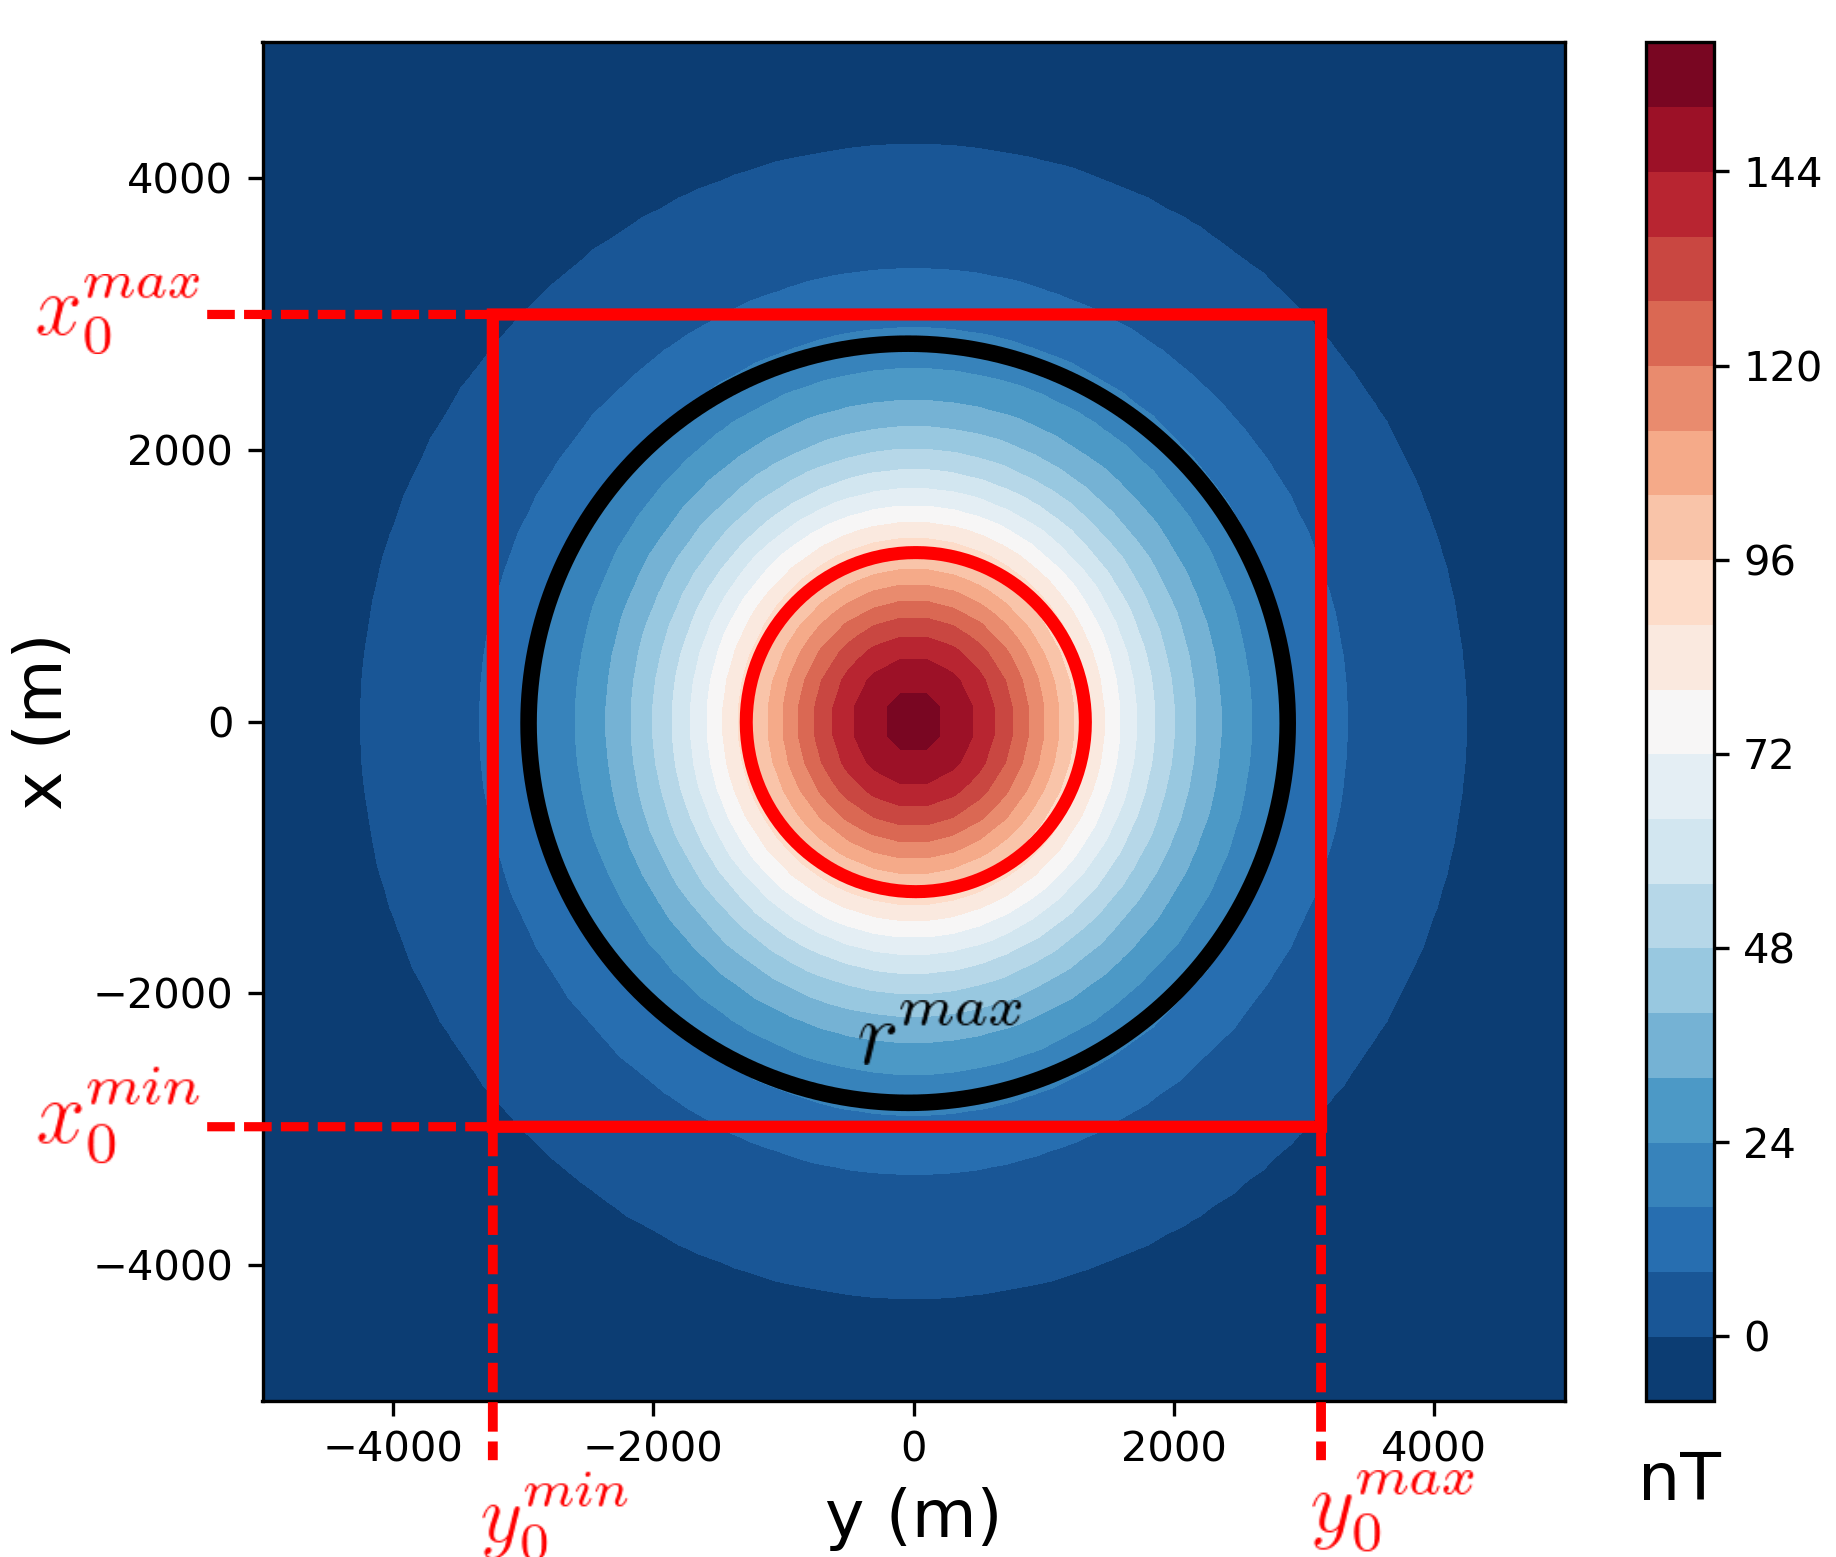
\includegraphics[scale=0.8]{rtp-example.png}
	\caption{Exemplo ilustrativo de anomalia de campo total reduzida ao polo para a definição dos limites do vínculo de desigualdades e aproximação inicial. O círculo preto representa o valor máximo $ r^{max} $ para os raios $r_j^k$, $j=1,\dots ,V$, $k=1,\dots ,L$. O retângulo vermelho representa a área composta pelos valores mínimos ($ x_0^{min} $ e $ y_0^{min} $) e máximos ($ x_0^{max} $ e $ y_0^{max} $) das coordenadas Cartesianas horizontais $ x_0^k $ e $ y_0^k $ da origem $ O^k $. Já o círculo vermelho representa o raio $r_j^k$ da aproximação inicial cilíndrica $ \hat{\mathbf{p}}_0 $.}
	\label{fig:rtp}
\end{figure}

Para definir o raio e as coordenadas horizontais do centro da aproximação inicial cilíndrica $ \hat{\mathbf{p}}_0 $, é escolhida a área circular que compreende a região onde a anomalia RTP é positiva e possui seu máximo.
O ideal aqui é que o raio da aproximação inicial $ \hat{\mathbf{p}}_0 $ coincida com a região de máximo gradiente da anomalia RTP, ou seja, onde se encontra a variação máxima desse dado que pode indicar os limites laterais da fonte alvo \citep{baranov1957}.
Essa definição não exige um rigor matemático muito acurado.
Depois de definir o raio e as coordenadas Cartesianas horizontais do centro da aproximação cilíndrica inicial $ \hat{\mathbf{p}}_0 $, devem ser escolhidos sua espessura de modo que a aproximação inicial seja mais profunda que a extensão vertical esperada fonte alvo.
A próxima etapa consiste em um modelagem direta da anomalia de campo total (Eq. \ref{eq:predicted-data-i}) com o intuito de ajustar o volume e definir os intervalos para a sua intensidade de magnetização total $m_{0}$ e a profundidade do topo $z_{0}$, as quais ajustam preliminarmente o dado observado $ \mathbf{d}^o $.
A Figura \ref{fig:prefit} exemplifica esse ajuste preliminar dos dados observados e os dados produzidos pela aproximação inicial $ \hat{\mathbf{p}}_0 $.
Note que essa modelagem direta é realizada antes de iniciar o processo de inversão e 
que o corpo cilíndrico resultante pode produzir um ajuste impreciso dos dados.

%FIGURA
\begin{figure}[!htb]
	\centering
	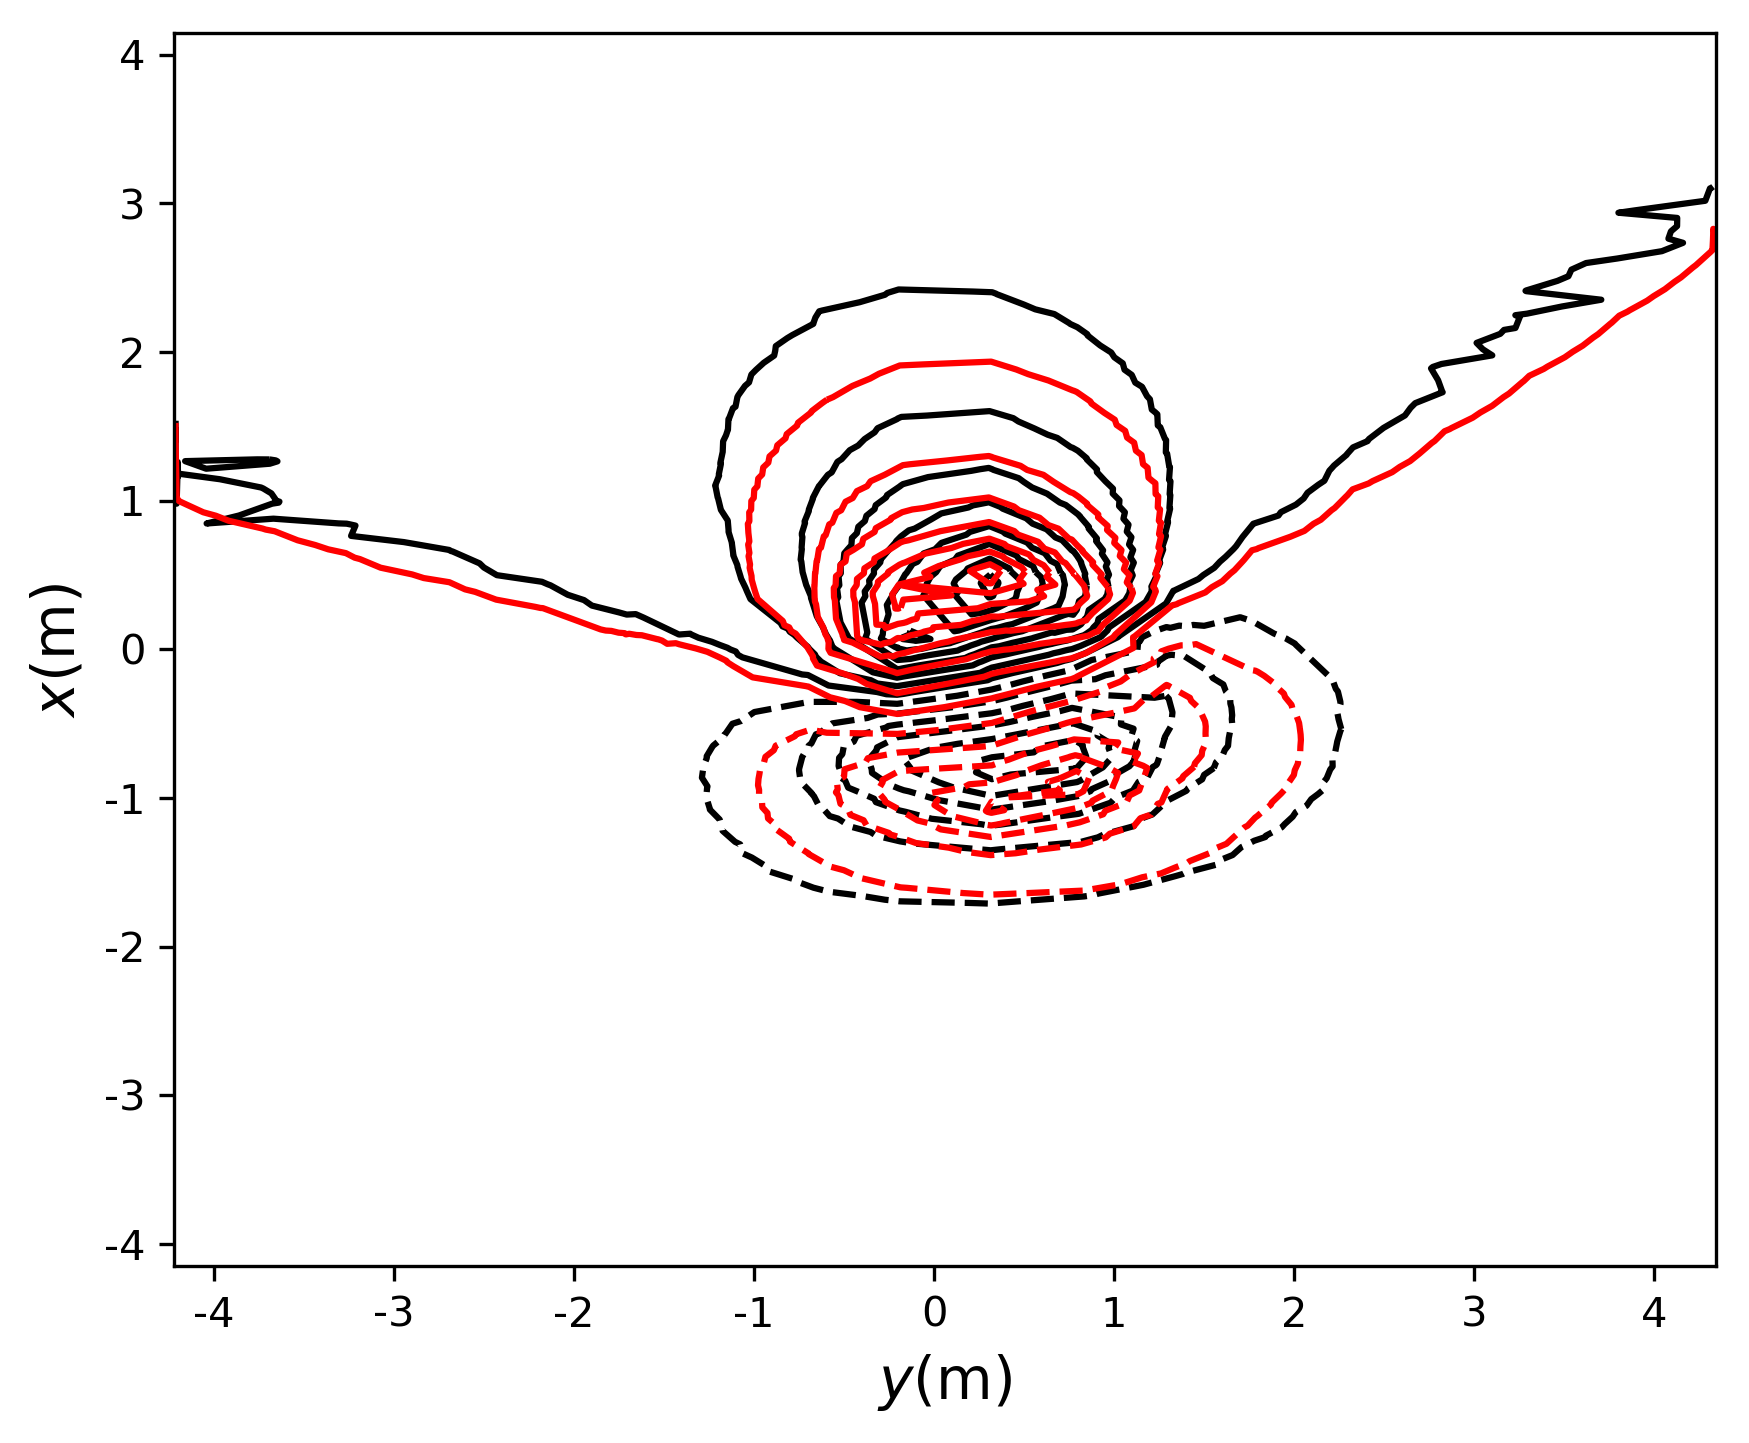
\includegraphics[scale=0.8]{prefitting.png}
	\caption{Exemplo ilustrativo de um ajuste preliminar entre anomalia de campo total observada (linhas pretas) e os dados produzidos pela da aproximação inicial $ \hat{\mathbf{p}}_0 $ (linhas vermelhas). Linhas contínuas representam dados positivos e linhas tracejadas representam dados negativos.}
	\label{fig:prefit}
\end{figure}

\section{Escolha dos pesos $\alpha_{1}-\alpha_{5}$}

Atribuir valores aos pesos $ \alpha_{\ell} $ (Eq. \ref{eq:gamma}) é uma etapa muito importante deste método.
Entretanto, não existe uma regra analítica para definí-los e seus valores podem ser dependentes das características particulares da configuração geológica onde o método está sendo aplicado \cite[]{silva-2001}.

Neste ponto, vale ressaltar que os pesos $ \alpha_{\ell}$ (eq. \ref{eq:gamma}) são quantidades com dimensão.
Note que as unidades da função data-misfit para a norma-2 e norma-1 dos resíduos (Eqs. \ref{eq:L2_misfit} e \ref{eq:L1_misfit}) são nT$^2$ e nT, respectivamente.
E as funções dos vínculos (Eqs. \ref{eq:phi1}, \ref{eq:phi2}, \ref{eq:phi3}, \ref{eq:phi4} e \ref{eq:phi5}) possuem unidade de m$^2$.
Por essa razão, a unidade dos pesos $ \alpha_{\ell} $ (Eq. \ref{eq:gamma}) é nT$^{2}/$m$^{2}$ para quando a função data-misfit é a norma-2 dos resíduos (Eq. \ref{eq:L2_misfit}) e nT$/$m$^{2}$ para o caso da utilização da norma-1 dos resíduos (Eq. \ref{eq:L1_misfit}).

A dimensão física dos pesos $ \alpha_{\ell}$ faz com que a solução do problema inverso seja variável.
Para tornar esses pesos comparáveis entre si, realiza-se a seguinte normalização sobre $ \alpha_{\ell} $:
\begin{equation}\label{eq:alphas}
\alpha_{\ell} = \tilde{\alpha}_\ell \frac{E_\phi}{E_\ell}, \quad \ell = 1,\dots, 5,
\end{equation}
em que $\tilde{\alpha}_\ell$ é um escalar positivo e $ E_\phi/E_\ell $ é um fator de normalização que permite que os $\tilde{\alpha}_\ell$ sejam independentes de unidades físicas utilizadas.
Nesta equação, $ E_\ell $ representa o traço da matriz Hessian $\mathbf{H}_{\ell}$ (eqs \ref{eq:phi1_gh}, \ref{eq:phi2_gh}, \ref{eq:phi3_gh}, \ref{eq:phi4_gh} e \ref{eq:phi5_gh}) do $ \ell $-ésima função de vínculo $\varphi_{\ell}(\mathbf{p})$ (eqs \ref{eq:phi1}, \ref{eq:phi2}, \ref{eq:phi3}, 
\ref{eq:phi4} e \ref{eq:phi5}).
A constante $E_\phi$ é o traço da matriz Hessiana $\mathbf{H}_{\phi}(\hat{\mathbf{p}}_{(0)})$ da função data-misfit $\phi(\mathbf{p})$ (Eqs. \ref{eq:L2_misfit} e \ref{eq:L1_misfit}) computada com a aproximação inicial $\hat{\mathbf{p}}_{(0)}$ para o vetor de parâmetros $ \mathbf{p} $ (Eq. \ref{eq:p-vector}) no início do algoritmo de inversão.
Note que o traço da matriz Hessiana $\mathbf{H}_{\ell}$ é adimensional e o traço da matriz Hessiana $\mathbf{H}_{\phi}(\hat{\mathbf{p}}_{(0)})$ tem unidade de nT$^{2}/$m$^{2}$ para a norma-2 e nT$ / $m$ ^2 $ para a norma-1.
Logo, os escalares positivos $\tilde{\alpha}_\ell$ na Equação \ref{eq:alphas} são quantidades adimensionais.

De acordo com essa estratégia empírica, os pesos $ \alpha_{\ell} $ 
(Eq. \ref{eq:gamma}) são redefinidos usando os escalares positivos $\tilde{\alpha}_\ell$ (eq. \ref{eq:alphas}), os quais são independentes de unidades físicas e menos dependentes das características particulares da configuração geológica.

\section{Considerações práticas}

Os valores atribuídos ao pesos adimensionais $\tilde{\alpha}_{1} - \tilde{\alpha}_{5}$ (eq. \ref{eq:alphas}) impactam significativamente os modelos estimados e não podem ser automaticamente escolhidos sem o julgamento do intérprete.
Baseado em experiência empírica, este trabalho sugere alguns procedimentos para a escolha desses parâmetros.

Os parâmetros $\tilde{\alpha}_1$ e $\tilde{\alpha}_2$ impõem informação a prior na forma da seção horizontal dos prismas.
O primeiro força todos os prismas a terem uma seção horizontal circular, enquanto o segundo força todos os prismas a terem uma seção horizontal parecida.
Geralmente, seus valores variam de $10^{-5}$ a $10^{-3}$ e diferem entre si de uma ordem de grandeza, no máximo.
O parâmetro $\tilde{\alpha}_3$ também varia de $10^{-5}$ a $10^{-3}$ e controla a posição relativa dos prismas adjacentes que formam o modelo interpretativo.
Um valore alto privilegia um corpo estimado vertical, enquanto um valor pequeno tende a gerar um corpo estimado inclinado.

O parâmetro $\tilde{\alpha}_4$ possui um significado puramente matemático e é usado somente para estabilizar as soluções do problema inverso.
Seu valor é escolhido como o menor possível.
O parâmetro $\tilde{\alpha}_7$ controla a extensão vertical total do corpo estimado.
Quanto maior é o seu valor, mais rasa é a profundidade da base estimada e vice versa.
Uma regra geral é começar com os valores iniciais $\tilde{\alpha}_1 = 10^{-4}$, $\tilde{\alpha}_2 = 10^{-4}$, $\tilde{\alpha}_3 = 10^{-4}$, $\tilde{\alpha}_4 = 10^{-7}$ e $\tilde{\alpha}_5 = 10^{-5}$, e mudá-los para refinar os resultados.
Finalmente, é importante enfatizar que  $\tilde{\alpha}_1 - \tilde{\alpha}_5$ (Eq. \ref{eq:alphas}) não são alterados ao longo das iterações do algortimo de inversão.

\section{Critério para escolha da melhor solução}
\label{sec:criterio}

Para selecionar a melhor entre as soluções L2 e L1, um critério numérico é utilizado.
A escolha da melhor solução é baseada em uma comparação entre os valores das funções dos vínculos $ \varphi_\ell $ multiplicados pelos pesos normalizados $ \alpha_\ell $, $ \ell=1,\dots,5 $, computados para ambas as soluções.
Tanto a solução L2 quanto a solução L1 possuem valores para as funções dos vínculos calculados pelas Equações \ref{eq:phi1}, \ref{eq:phi2}, \ref{eq:phi3}, \ref{eq:phi4} e \ref{eq:phi5}.
Os pesos normalizados $ \alpha_\ell $, $ \ell=1,\dots,5 $, são definidos pela a Equação \ref{eq:alphas}. 
Quando a função do um vínculo multiplicada pelo seu peso normalizado associado $ \alpha_\ell \varphi_\ell  $, $ \ell=1,\dots,5 $, assume um valor pequeno significa que a informação a priori introduzida foi bem incorporada à inversão, ou seja, a solução final admite uma forma que minimiza estas quantidades.
Por exemplo, uma solução cilíndrica vai apresentar valores de $ \varphi_1 $, $ \varphi_2 $ e $ \varphi_3 $ iguais a zero independentemente do valor de seus respectivos pesos normalizados $ \alpha_1 $, $ \alpha_2 $ e $ \alpha_3 $, uma vez que todos os raios $ r^k_j $, $ j=1, \dots, V $, $ k=1,\dots,L $, e todas as coordenadas Cartesianas horizontais $ (x^k_0, y^k_0) $ das origens $ O^k $ de todos os $ L $ prismas que compõem o modelo interpretativo serão iguais (Eqs. \ref{eq:phi1}, \ref{eq:phi2} e \ref{eq:phi3}).
Portanto, a partir desses valores, a melhor solução é aquela que possuir a maior quantidade de menores valores das funções dos vínculos multiplicados pelos pesos normalizados em comparação à outra.
  \chapter{Aplicação a dados sintéticos}

Todos os dados sintéticos apresentados neste capítulo foram simulados na presença de um campo geomagnético principal com inclinação $ I_0 = -21,5 $ e declinação $ D_0 = -18,7 $.


\section{Modelo simples}

Foi simulado um corpo geológico simples imerso em meio não magnético (prismas azuis nas Figuras 
\ref{fig:simple_model}, \ref{fig:simple_l2_result} e \ref{fig:simple_l1_result})
que representa a fonte alvo 3D com profundidade do topo em $0$ m, profundidade da base em $1600$ m, centro em $ (x_0, y_0) = (0, 0) $ e um vetor de magnetização total constante com inclinação $-50^{\circ}$, declinação $9^{\circ}$, e intensidade $9$ A/m.
Esse modelo é composto de $ 8 $ prismas com $ 20 $ vértices cada e raios que diminuem com a profundidade: ($ 1920 $ m, $ 1760 $ m, $ 1600 $ m, $ 1440 $ m, $ 1280 $ m, $ 1120 $ m, $ 960 $ m, $ 800 $ m).
Recuperar a geometria desse corpo é uma tarefa relativamente simples para este método porque ele possui um alinhamento vertical e suas fatias horizontais mostram uma forma circular que diminui de tamanho ao longo da profundidade, assim, é possível notar que o corpo satisfaz perfeitamente quase todos os vínculos impostos neste método.
A anomalia de campo total (Figura \ref{fig:simple_model}a) produzida pela fonte alvo foi calculada em $1939$ pontos localizados sobre uma malha irregular com linhas que simulam um levantamento aéreo (Figura \ref{fig:simple_model}b) no plano $ z=-150 $ m. Esses dados sintéticos foram contaminados com um ruído Gaussiano pseudo-aleatório de média zero e desvio padrão igual a $5$ nT.
O método foi aplicado para inverter esse dado contaminado com ruído e obter soluções L2 e L1.
Para cada tipo de solução, foram geradas $36$ soluções L2 e $36$ soluções L1, 
todas elas foram obtidas com a mesma malha de varredura $6 \times 6$ de profundidades do topo $z_{0}$ e intensidade de magnetização total $m_{0}$.
A melhor solução L2 e L1 são definidas como aquelas que produzem o menor valor da função objetivo para cada caso.

A Figura \ref{fig:simple_model_rtp} mostra a anomalia RTP obtida via camada equivalente a partir da anomalia de campo total contaminada com ruído (Figura \ref{fig:simple_model}a) e 
a projeção horizontal das aproximações iniciais $\hat{\mathbf{p}}_{(0)}$ 
usadas nas sucessivas inversões (Figuras \ref{fig:simple_l2_result} e 
\ref{fig:simple_l1_result}).
As aproximações iniciais são compostas de $ L= 5$ prismas com $ V = 20 $ vértices, mesma direção de magnetização do corpo verdadeiro, espessura $ dz=350 $ m e centro em $ (x_0, y_0) = (0, 0) $.
A Figura \ref{fig:simple_l2_result}a mostra que a melhor solução L2 foi obtida através dos valores verdadeiros da profundidade do topo $z_{0}$ e intensidade de magnetização total $m_{0}$.
Essa solução L2 produz um ótimo ajuste dos dados (Figura \ref{fig:simple_l2_result}b), possui uma profundidade da base em $1581.5$ m e também recupera a geometria do corpo verdadeiro (Figura \ref{fig:simple_l2_result}d).
A Figura \ref{fig:simple_l1_result} mostra um resultado similar para a solução L1, porém com um ajuste dos dados e geometria inferiores aos da solução L2. A profundidade da base foi estimada em $1412,9$ m.
Podemos observar que nesse teste ambas as abordagens L2 e L1 foram bem sucedidas em estimar a forma do corpo e recuperam as feições principais da fonte alvo.
Entretanto, nesse caso, a Tabela \ref{tab:simple} mostra que solução L2 foi ligeiramente superior à solução L1 utilizando o critério apresentado na Seção \ref{sec:criterio}.
Todas as soluções L2 e L1 produzidas neste teste foram obtidas usando o seguinte conjunto de pesos normalizados $\tilde{\alpha}_{\ell}$ (Equação \ref{eq:alphas}): 
$\tilde{\alpha}_{1} = 10^{-3}$, $\tilde{\alpha}_{2} = 10^{-4}$, 
$\tilde{\alpha}_{3} = 10^{-4}$, $\tilde{\alpha}_{4} = 10^{-6}$, e 
$\tilde{\alpha}_{5} = 10^{-4}$. 
É importante notar que, mesmo a solução L2 sendo superior à solução L1, não há diferenças significativas entre as soluções L2 e L1 obtidas pelo método.

\begin{table}[h]\label{tab:simple}
	\caption{Valores dos vínculos na iteração final para as melhores soluções L2 e L1 da aplicação ao corpo complexo na presença de uma fonte não-alvo pequena (Eqs. \ref{eq:phi1}, \ref{eq:phi2}, \ref{eq:phi3}, \ref{eq:phi4} e \ref{eq:phi5}).}
	\centering
	\vspace{0.5cm}
	\begin{tabular}{c|ccccc}
		Vínculo & $ \varphi _1 $ & $ \varphi _2 $ &  $ \varphi _3 $ &  $ \varphi _4 $ &  $ \varphi _5 $ \\
		\hline
		Solução L2 & $ 2,09 $ & $ 17,78 $ & $ 7,42\times 10^{-3} $ & $7,30 $ & $ 18,78 $ \\ 
		Solução L1 & $ 3,99 $ & $ 11,96 $ & $ 0,21 $ & $7,58$ & $ 14,75 $
	\end{tabular}
\end{table}

\pagebreak

\begin{figure}[!htb]
	\centering
	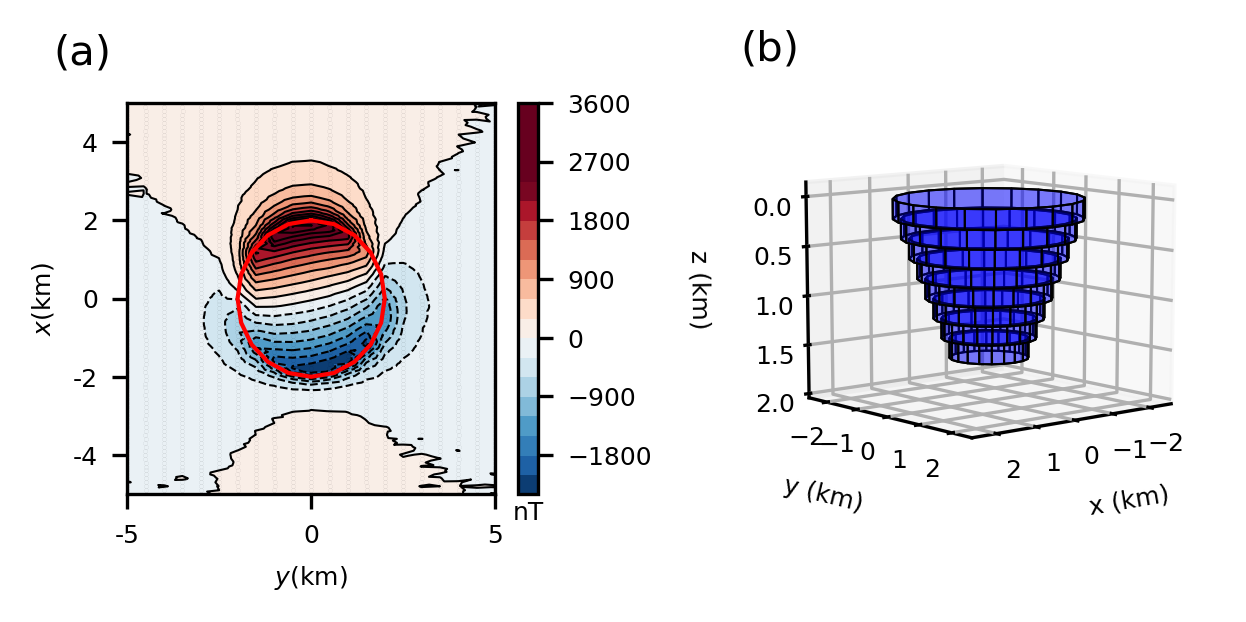
\includegraphics[width=\textwidth]{simple_model_data.png}
	\caption{Modelo simples. (a) Anomalia de campo total contaminada com ruído produzida pela fonte simples (prismas azuis mostrados nos painel b). Os pontos pretos representam os pontos de observação. O círculo vermelho representa a projeção horizontal da aproximação inicial $\hat{\mathbf{p}}_{(0)}$ (prismas vermelhos nas Figuras
		\ref{fig:simple_l2_result}c). %e \ref{fig:simple_l1_result}c). 
		(b) Visualização em perspectiva do modelo da fonte simples representada pelos prismas azuis.
	}
	\label{fig:simple_model}
\end{figure}

\pagebreak

\begin{figure}[!htb]
	\centering
	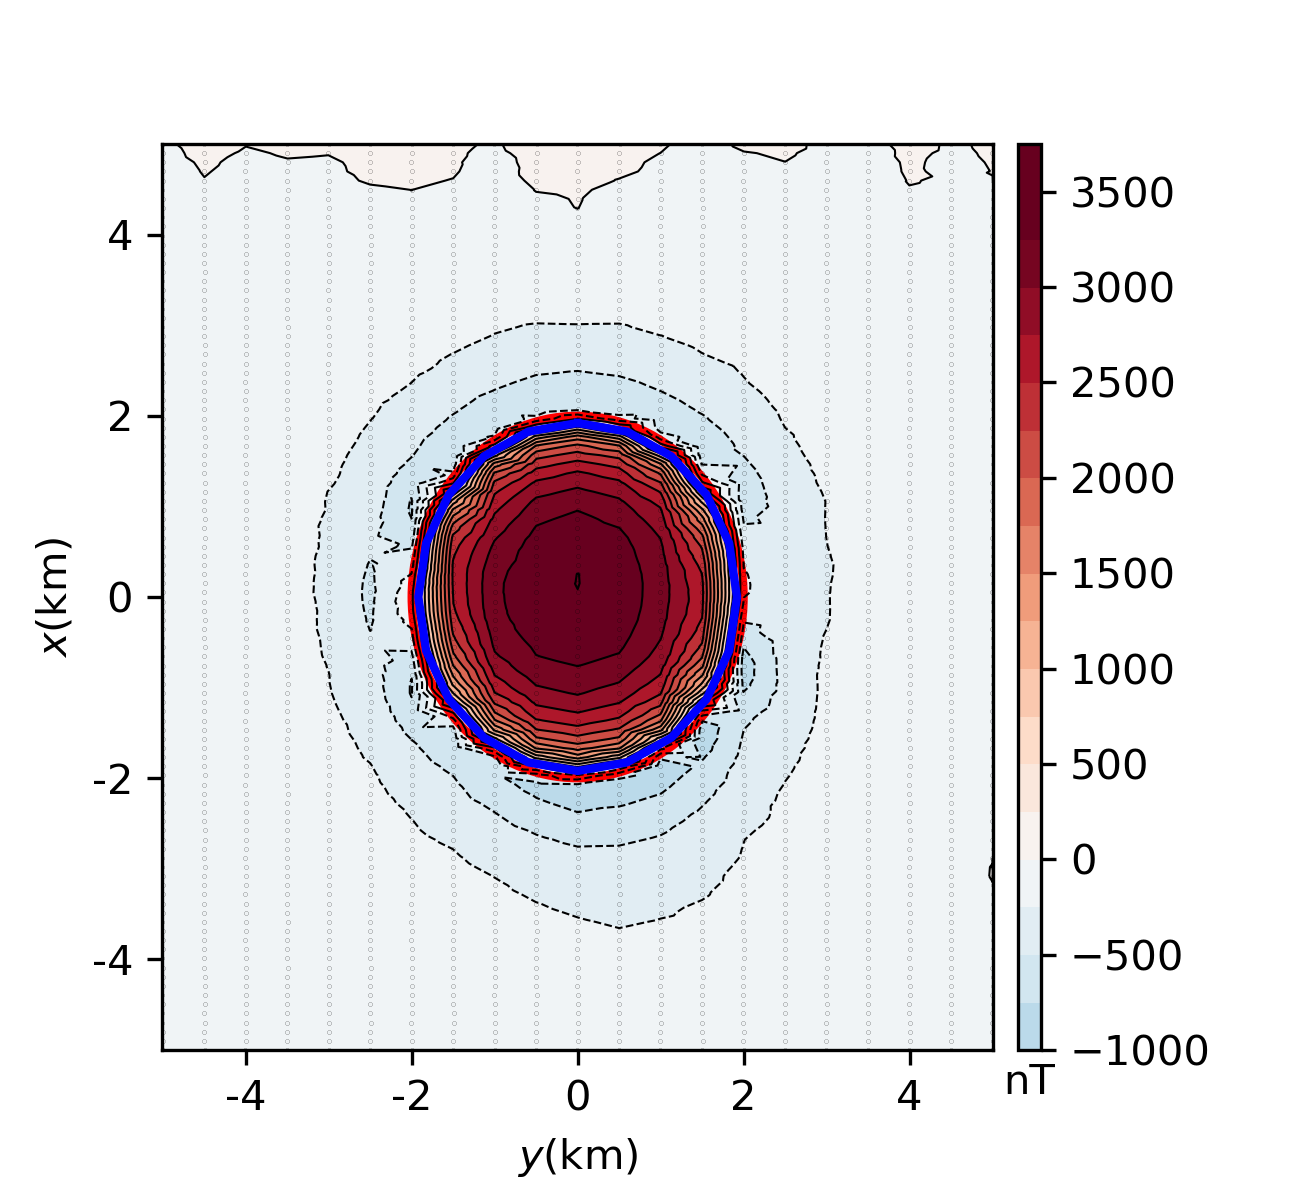
\includegraphics[width=\textwidth]{simple_rtp.png}
	\caption{Anomalia RTP produzida pela fonte simples. 
		A anomalia RTP mostra valores predominantemente positivos logo acima da fonte simples. Os pontos pretos representam os pontos de observação. As linhas azuis e vermelhas correspondem, respectivamente, às projeções horizontais da porção mais rasa da fonte alvo e da aproximação inicial utilizada nas inversões subsequentes (prismas vermelhos nas Figuras \ref{fig:simple_l2_result}c e 
		\ref{fig:simple_l1_result}c).
	}
	\label{fig:simple_model_rtp}
\end{figure}

\pagebreak

\begin{figure}[!htb]
	\centering
	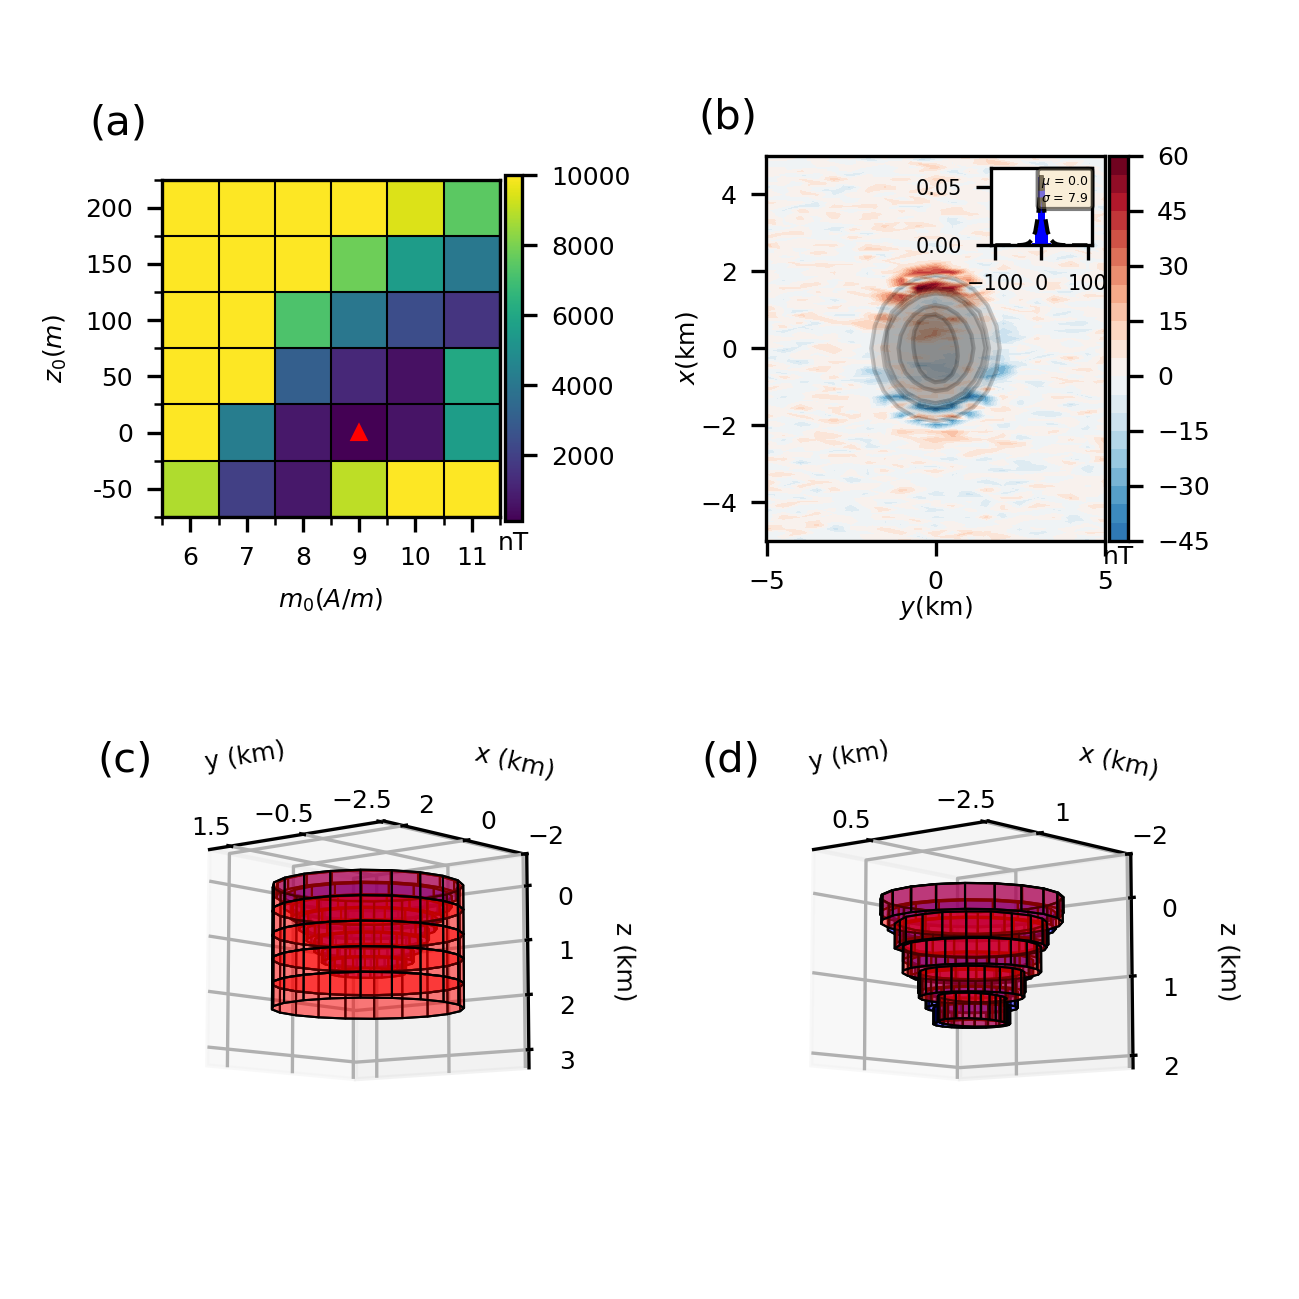
\includegraphics[width=\textwidth]{simple-l2-solution.png}
	\caption{Soluções L2 obtidas para o modelo da fonte simples. 
		(a) Mapa discreto da função objetivo produzida pelos modelos obtidos a partir da varredura de valores de profundidade do topo $z_{0}$ e intensidade de magnetização total $m_{0}$. 
		O triângulo vermelho representa os valores verdadeiros para $m_{0}$ e $z_{0}$, assim como os valores que definem a melhor solução L2.
		(b) Resíduos entre os dados contaminados com ruído (Figura \ref{fig:simple_model}a) 
		e os dados preditos (não mostrados) produzidos pela melhor solução L2 (prismas vermelhos no painel d). 
		O histograma dos resíduos inserido em (b) mostra a curva Gaussiana ajustada (linha tracejada).
		Os polígonos cinzas representam as projeções horizontais de todos os prismas que compõe a melhor solução. 
		(c) e (d) Visualização em perspectiva da aproximação inicial (prismas vermelhos) e 
		a melhor solução (prismas vermelhos), respectivamente. Os prismas azuis são o modelo da fonte simples. 
	}
	\label{fig:simple_l2_result}
\end{figure}
\pagebreak

\begin{figure}[!htb]
	\centering
	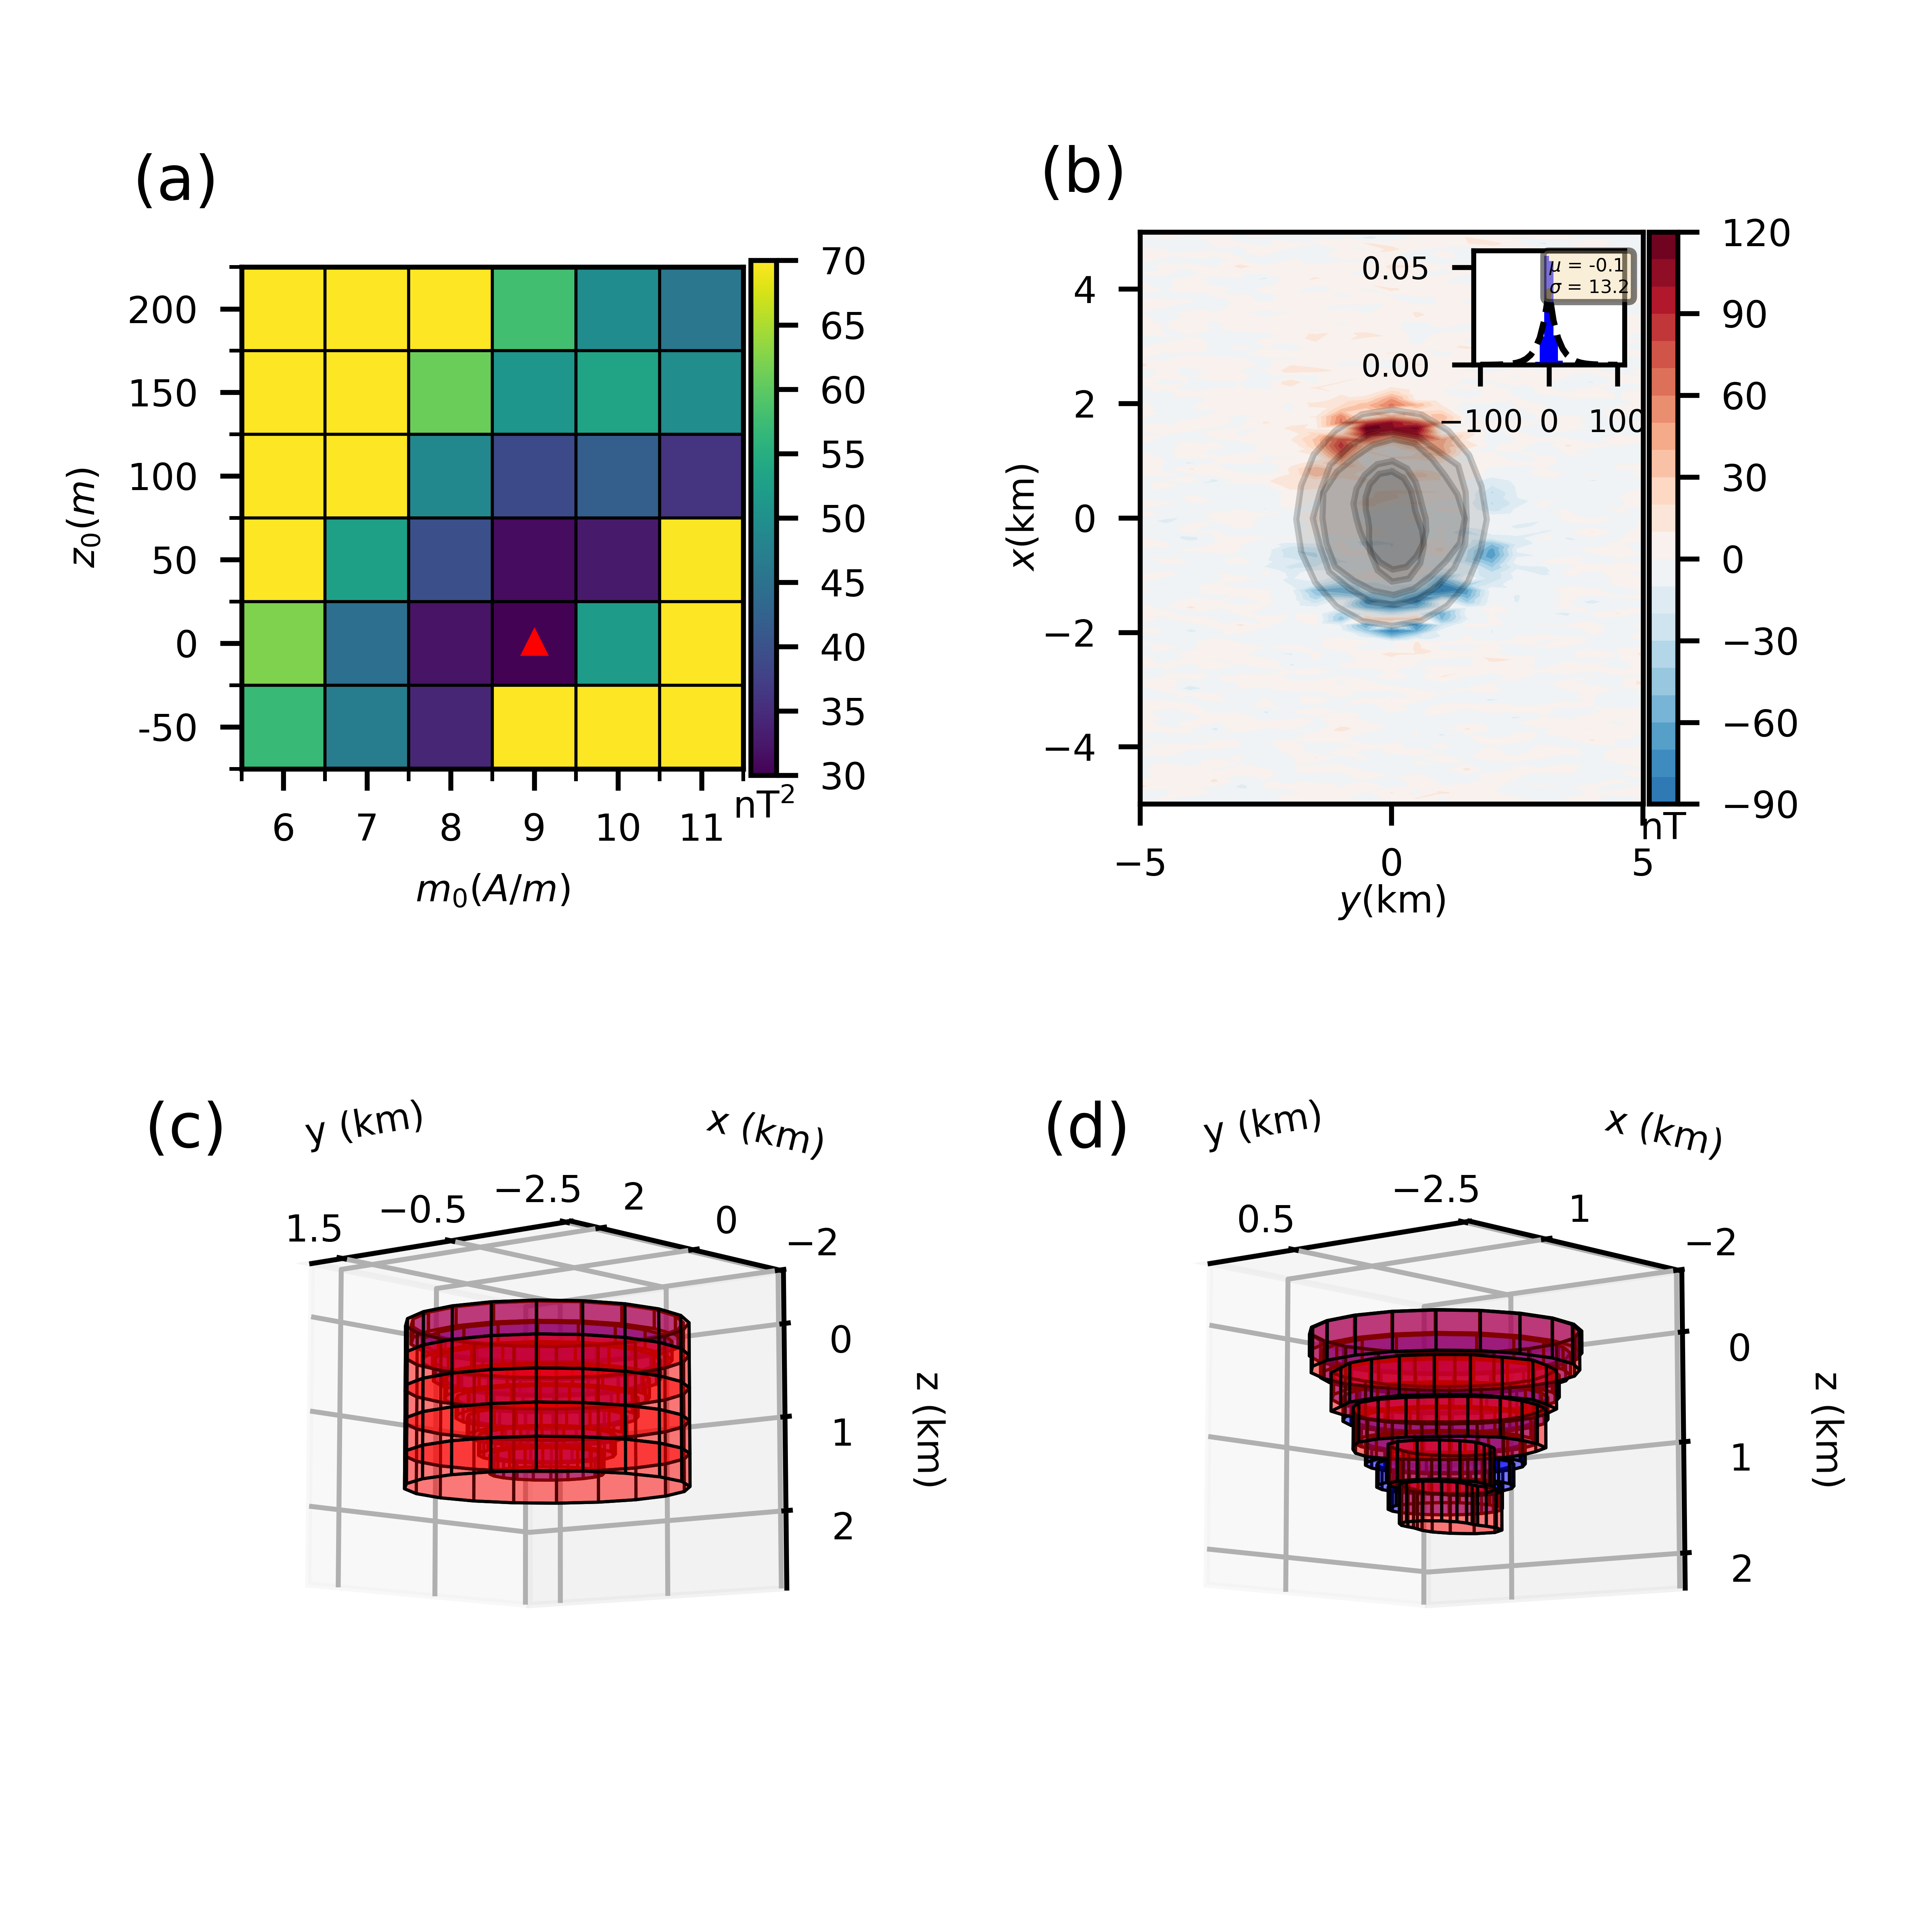
\includegraphics[width=\textwidth]{simple-l1-solution.png}
	\caption{Soluções L1 obtidas para o modelo da fonte simples. 
		(a) Mapa discreto da função objetivo produzida pelos modelos da malha de varredura para valores de profundidade do topo $z_{0}$ e intensidade de magnetização total $m_{0}$. 
		O triângulo vermelho representa os valores verdadeiros para $m_{0}$ e $z_{0}$, assim como os valores que definem a melhor solução L1.
		(b) Resíduos entre os dados contaminados com ruído (Figura \ref{fig:simple_model}a) 
		e os dados preditos (não mostrados) produzidos pela melhor solução L1 (prismas vermelhos no painel d). 
		O histograma dos resíduos inserido em (b) mostra a curva Laplaciana ajustada (linha tracejada).
		Os polígonos cinzas representam as projeções horizontais de todos os prismas que compõe a melhor solução. 
		(c) e (d) Visualização em perspectiva da aproximação inicial (prismas vermelhos) e 
		a melhor solução (prismas vermelhos), respectivamente. Os prismas azuis são o modelo da fonte simples. 
	}
	\label{fig:simple_l1_result}
\end{figure}

\pagebreak

\section{Modelo inclinado}

Para verificar se o método é capaz de recuperar um corpo que possui um mergulho de baixo ângulo $\approx 26,5^\circ $, foi simulado um corpo geológico inclinado imerso em meio não magnético (prismas azuis nas Figuras 
\ref{fig:inclined_model}, \ref{fig:inclined_l2_result} e \ref{fig:inclined_l1_result})
que representa a fonte alvo 3D com profundidade do topo em $0$ m, profundidade da base em $3040$ m, centro em $ (x_0, y_0) = (-300, 600) $ e um vetor de magnetização total constante com inclinação $-50^{\circ}$, declinação $9^{\circ}$, e intensidade $9$ A/m.
Esse modelo é composto de $ 8 $ prismas com $ 20 $ vértices.
Recuperar a geometria desse corpo simulado é uma tarefa relativamente complicada para este método porque ele possui um mergulho baixo em uma direção aproximadamente N-S e suas fatias horizontais mostram uma forma irregular que varia de tamanho ao longo da profundidade, assim, é possível notar que o corpo não satisfaz os vínculos impostos neste método.
A anomalia de campo total (Figura \ref{fig:inclined_model}a) produzida pela fonte alvo foi calculada em $1674$ pontos localizados sobre uma malha irregular sobre uma superfície ondulada com linhas que simulam um levantamento aéreo (Figura \ref{fig:inclined_model}b). Esses dados sintéticos foram contaminados com um ruído Gaussiano pseudo-aleatório de média zero e desvio padrão igual a $5$ nT.
O método foi aplicado para inverter esse dado contaminado com ruído e obter soluções L2 e L1.
Para cada tipo de solução, foram geradas $36$ soluções L2 e $36$ soluções L1, 
todas elas foram obtidas com a mesma malha de varredura $6 \times 6$ de profundidades do topo $z_{0}$ e intensidade de magnetização total $m_{0}$.
A melhor solução L2 e L1 são definidas como aquelas que produzem o menor valor da função objetivo para cada caso.

A Figura \ref{fig:inclined_model_rtp} mostra a anomalia RTP obtida a partir da anomalia de campo total contaminada com ruído (Figura \ref{fig:inclined_model}a) e 
a projeção horizontal das aproximações iniciais $\hat{\mathbf{p}}_{(0)}$ 
usadas nas sucessivas inversões (Figuras \ref{fig:inclined_l2_result} e 
\ref{fig:inclined_l1_result}).
As aproximações iniciais são compostas de $ L= 5$ prismas com $ V = 20 $ vértices, mesma direção de magnetização do corpo verdadeiro, espessura $ dz=350 $ m e centro em $ (x_0, y_0) = (-200, 0) $.
A Figura \ref{fig:inclined_l2_result}a mostra que a melhor solução L2 obtida superestima a profundidade do topo $z_{0}$ e acerta o valor da intensidade de magnetização total $m_{0}$ verdadeira. Essa solução L2 produz um ótimo ajuste dos dados (Figura \ref{fig:inclined_l2_result}b), possui uma profundidade da base em $3453,0$ m e também recupera a geometria do corpo verdadeiro (Figura \ref{fig:inclined_l2_result}d).
A Figura \ref{fig:inclined_l1_result} mostra um resultado similar para a solução L1, porém a profundidade da base estimada em $3107,2$ m foi muito próxima da verdadeira.
Podemos observar que nesse teste ambas as abordagens L2 e L1 foram bem sucedidas em estimar a forma do corpo e recuperam as feições principais da fonte alvo. Entretanto, nesse caso, a Tabela \ref{tab:inc} mostra que a solução L1 foi superior à solução L2.
Todas as soluções L2 produzidas neste teste foram obtidas usando o seguinte conjunto de pesos normalizados $\tilde{\alpha}_{\ell}$ (Equação \ref{eq:alphas}): 
$\tilde{\alpha}_{1} = 10^{-3}$, $\tilde{\alpha}_{2} = 10^{-3}$, 
$\tilde{\alpha}_{3} = 10^{-6}$, $\tilde{\alpha}_{4} = 10^{-6}$, e 
$\tilde{\alpha}_{5} = 10^{-5}$. 
Já as soluções L1 foram obtidas utilizando o conjunto: 
$\tilde{\alpha}_{1} = 10^{-4}$, $\tilde{\alpha}_{2} = 10^{-4}$, 
$\tilde{\alpha}_{3} = 10^{-6}$, $\tilde{\alpha}_{4} = 10^{-6}$, e 
$\tilde{\alpha}_{5} = 10^{-5}$.
É importante notar que, mesmo a solução L1 sendo superior à solução L2, não há diferenças significativas entre as soluções L2 e L1 obtidas pelo método.

\begin{table}[h]\label{tab:inc}
	\caption{Valores dos vínculos na iteração final para as melhores soluções L2 e L1 da aplicação ao corpo complexo na presença de uma fonte não-alvo pequena (Eqs. \ref{eq:phi1}, \ref{eq:phi2}, \ref{eq:phi3}, \ref{eq:phi4} e \ref{eq:phi5}).}
	\centering
	\vspace{0.5cm}
	\begin{tabular}{c|ccccc}
		Vínculo & $ \varphi _1 $ & $ \varphi _2 $ &  $ \varphi _3 $ &  $ \varphi _4 $ &  $ \varphi _5 $ \\
		\hline
		Solução L2 & $ 3,21 $ & $ 7,97 $ & $ 0,10 $ & $0,17 $ & $ 0,62 $ \\ 
		Solução L1 & $ 0,31 $ & $ 0,56 $ & $ 0,10 $ & $0,18$ & $ 0,47 $
	\end{tabular}
\end{table}

\pagebreak

\begin{figure}[!htb]
	\centering
 	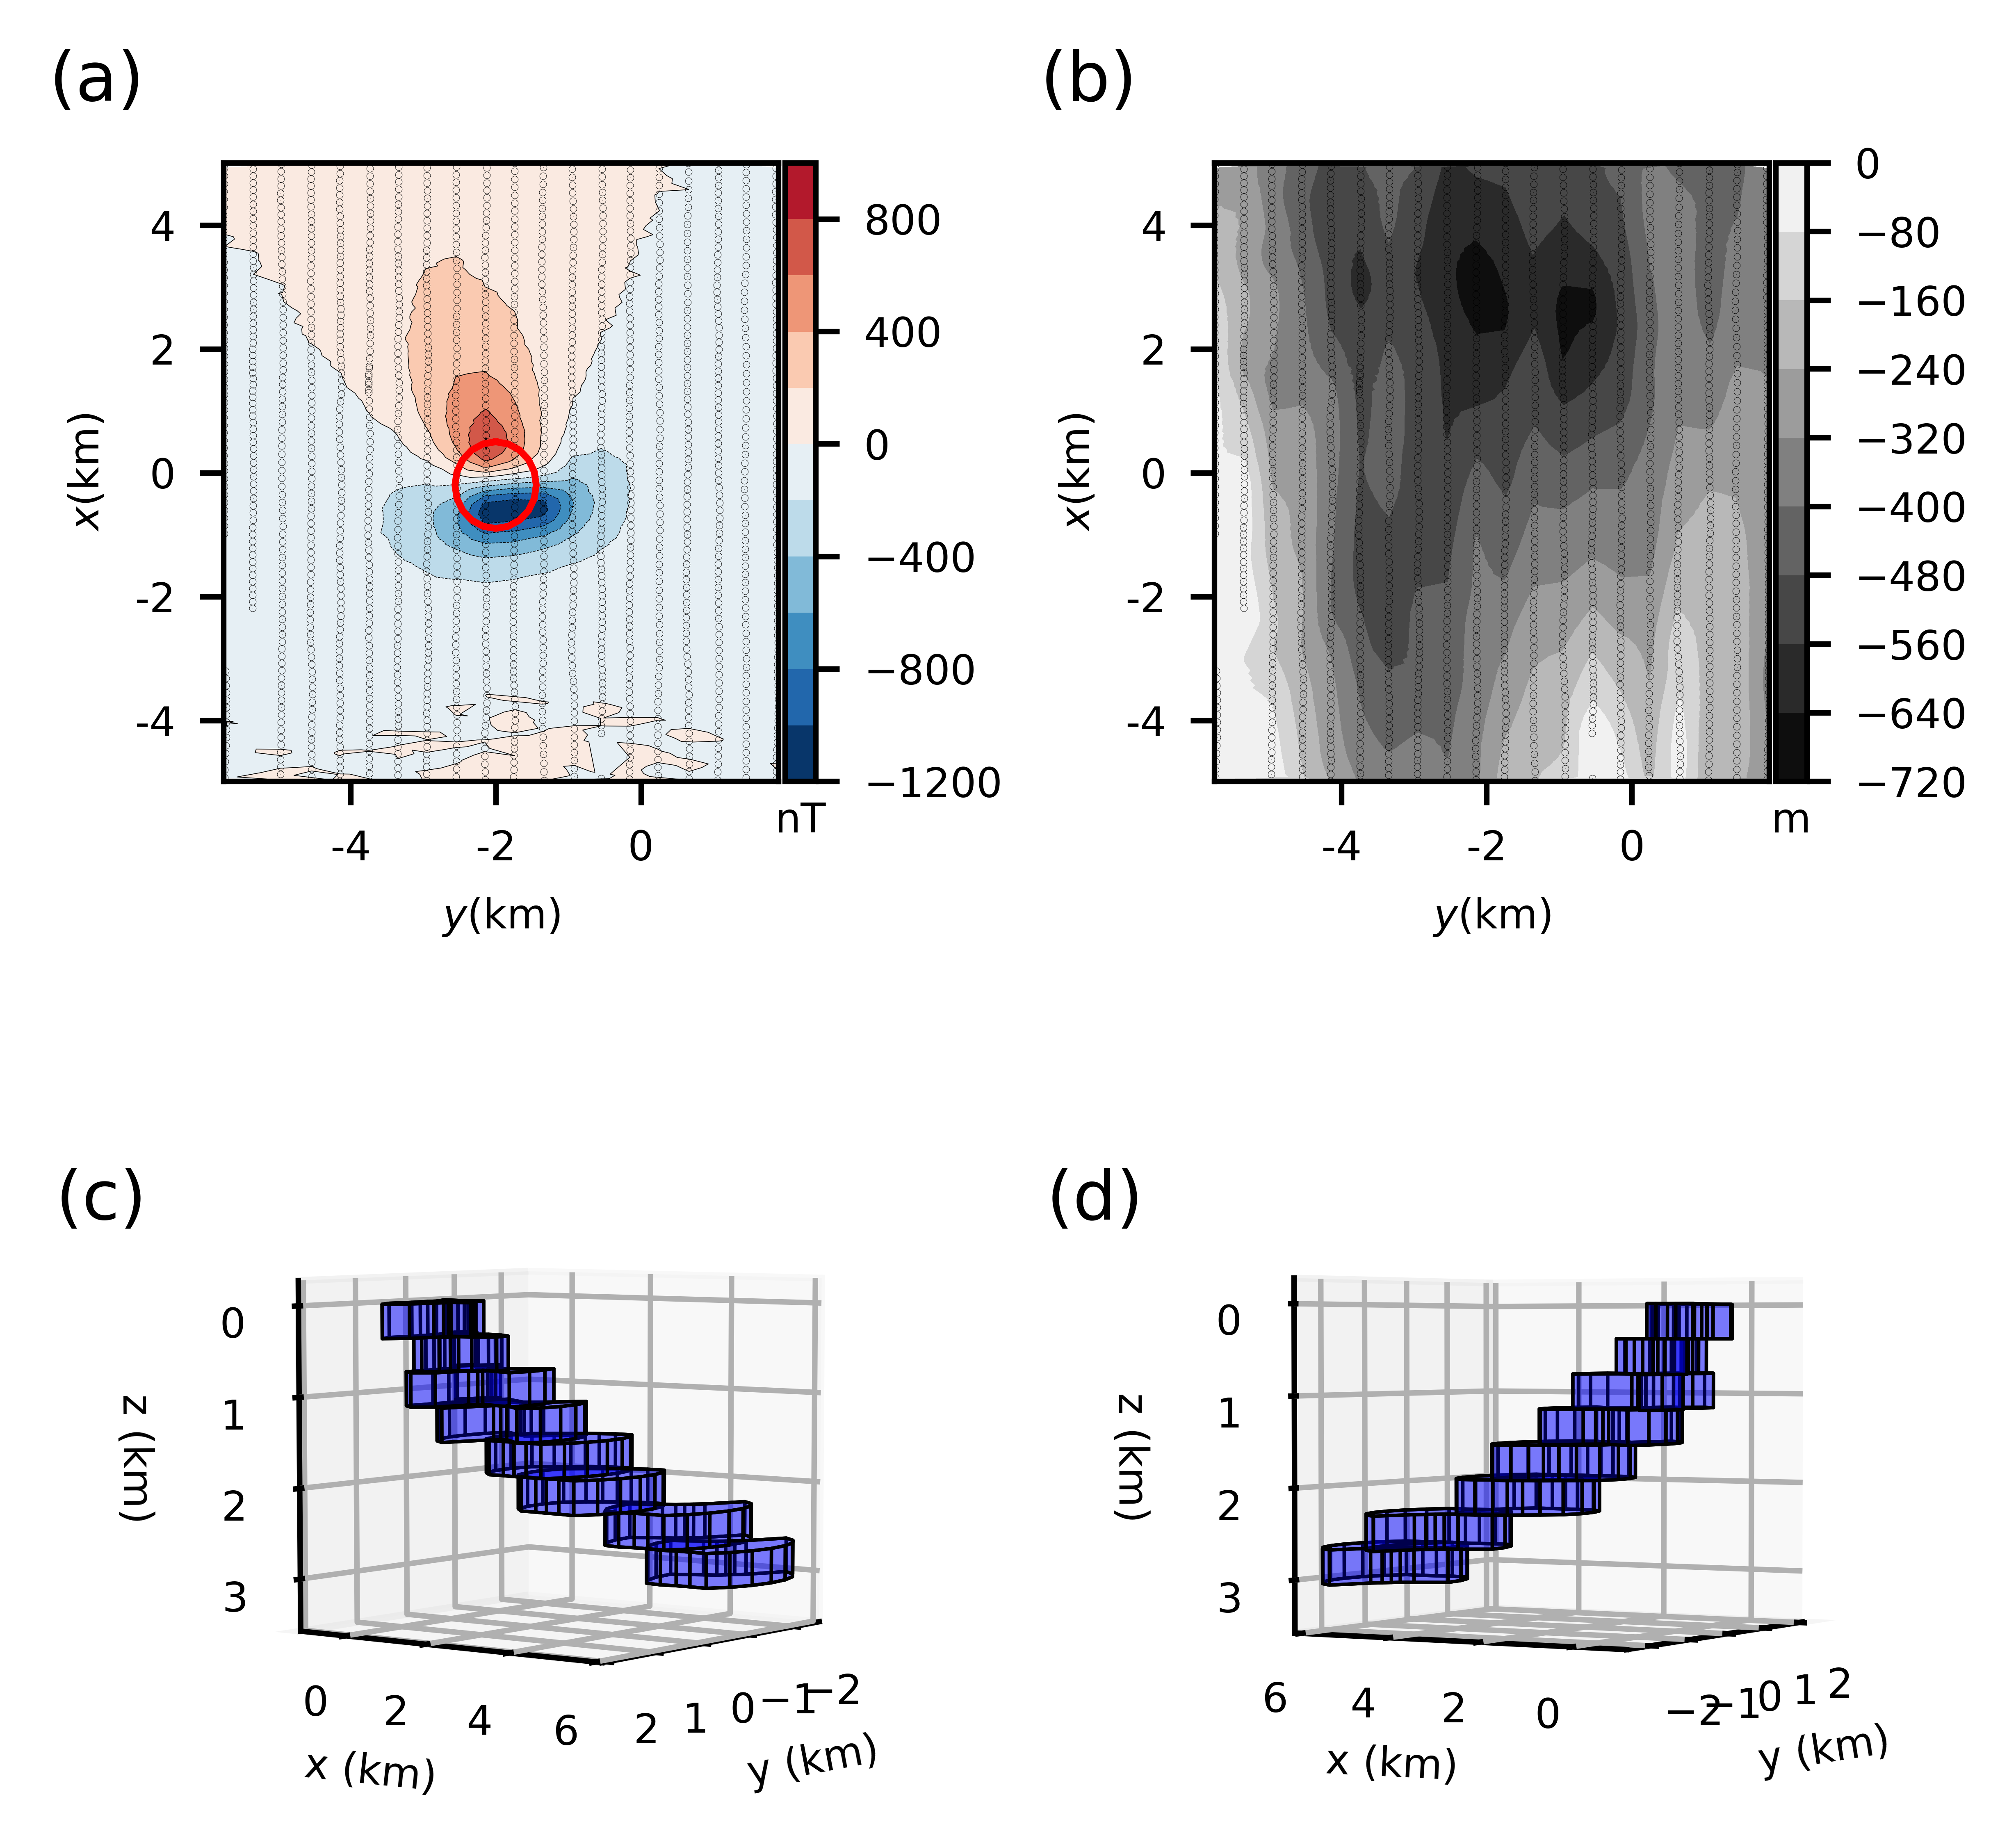
\includegraphics[width=\textwidth]{inclined_model_data.png}
	\caption{Modelo inclinado. (a) Anomalia de campo total contaminada com ruído produzida pela fonte alvo (prismas azuis mostrados nos painéis c e d). Os pontos pretos representam os pontos de observação. O círculo vermelho representa a projeção horizontal da aproximação inicial $\hat{\mathbf{p}}_{(0)}$ (prismas vermelhos nas Figuras
		\ref{fig:inclined_l2_result}c e \ref{fig:inclined_l1_result}c). (b) Coordenadas verticais dos pontos de observação que simulam um levantamento aéreo.
		(c) e (d) Visualizações em perspectiva do modelo da fonte alvo representada pelos prismas azuis.
	}
	\label{fig:inclined_model}
\end{figure}
\pagebreak

\begin{figure}[!htb]
	\centering
	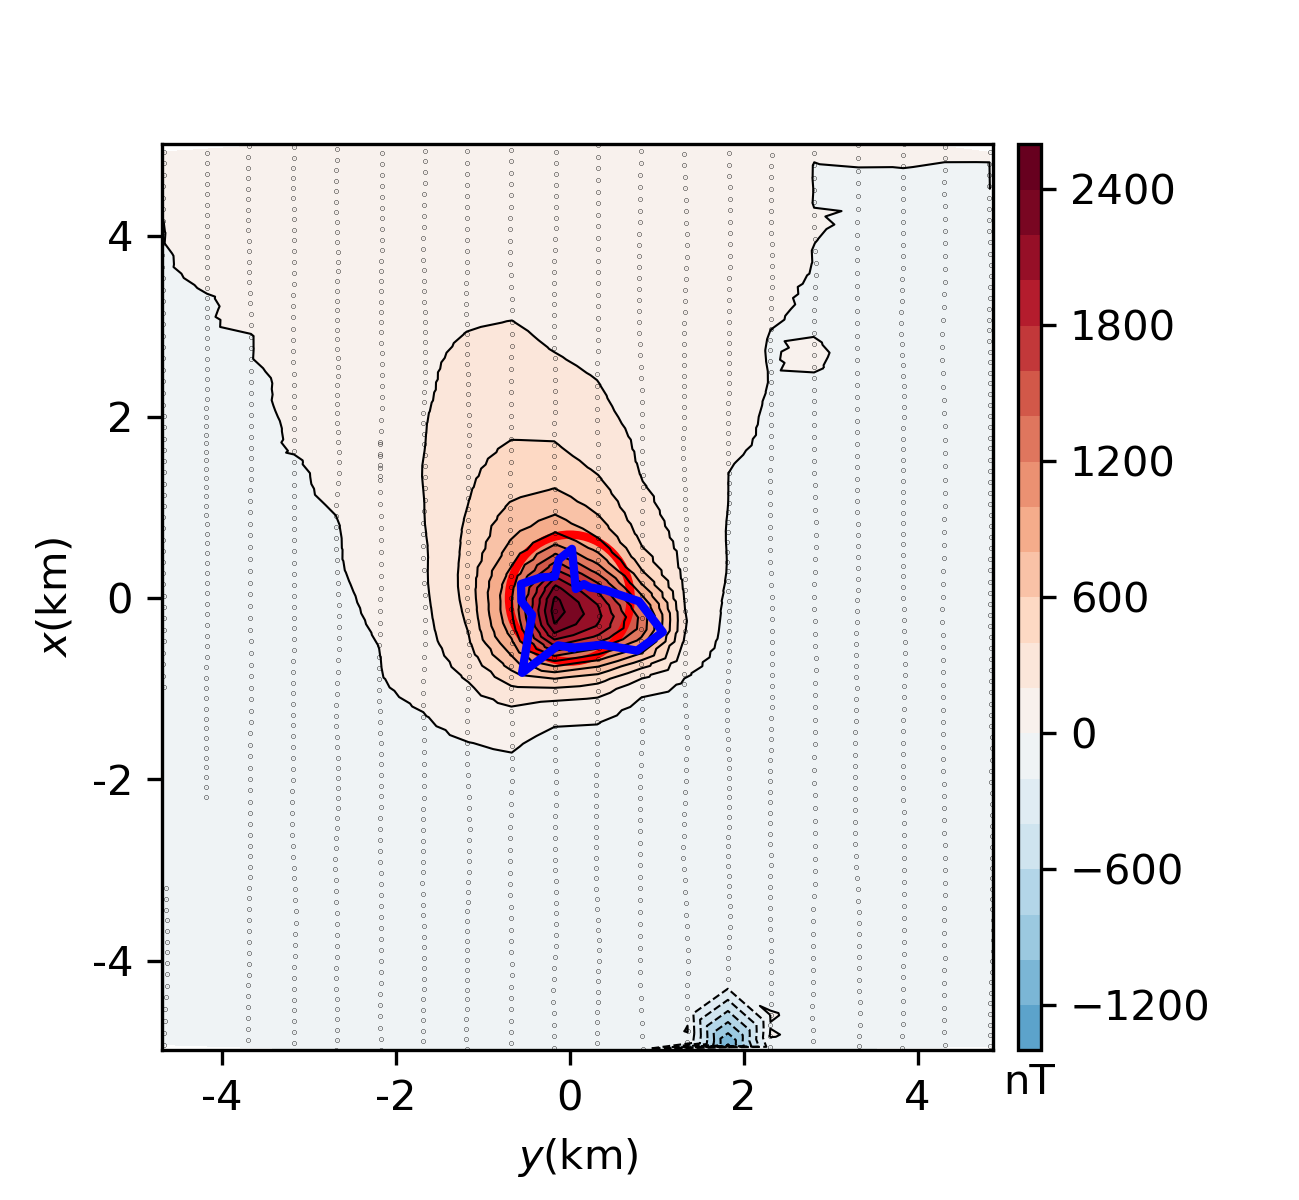
\includegraphics[width=\textwidth]{inclined_rtp.png}
	\caption{Anomalia RTP produzida pela fonte alvo. 
		A anomalia RTP mostra valores predominantemente positivos logo acima da fonte alvo. Os pontos pretos representam os pontos de observação. As linhas azuis e vermelhas correspondem, respectivamente, às projeções horizontais da porção mais rasa da fonte alvo e da aproximação inicial utilizada nas inversões subsequentes (prismas vermelhos nas Figuras \ref{fig:inclined_l2_result}c e 
		\ref{fig:inclined_l1_result}c).
	}
	\label{fig:inclined_model_rtp}
\end{figure}

\pagebreak

\begin{figure}[!htb]
	\centering
	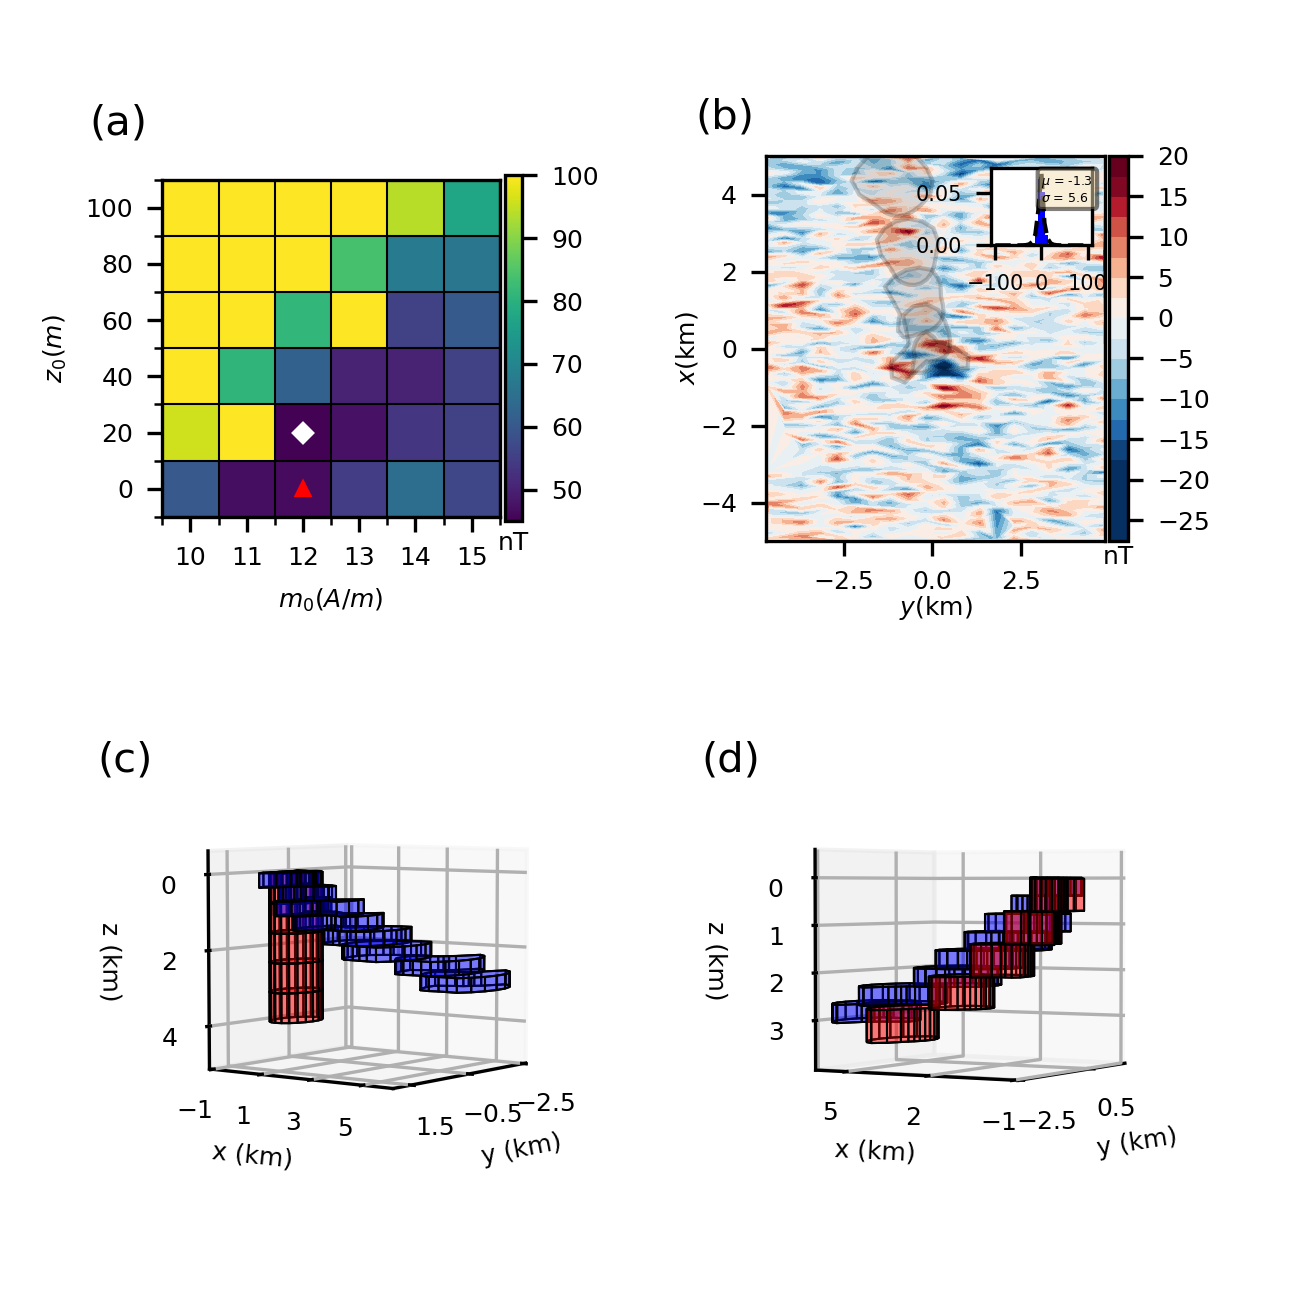
\includegraphics[width=\textwidth]{inclined-l2-solution.png}
	\caption{Soluções L2 obtidas para o modelo inclinado. 
		(a) Mapa discreto da função objetivo produzida pelos modelos obtidos a partir da varredura de valores de profundidade do topo $z_{0}$ e intensidade de magnetização total $m_{0}$. 
		O triângulo vermelho representa os valores verdadeiros para $m_{0}$ e $z_{0}$, enquanto o losango branco definem os valores para a melhor solução L2.
		(b) Resíduos entre os dados contaminados com ruído (Figura \ref{fig:inclined_model}a) 
		e os dados preditos (não mostrados) produzidos pela melhor solução L2 (prismas vermelhos no painel d). 
		O histograma dos resíduos inserido em (b) mostra a curva Gaussiana ajustada (linha tracejada).
		Os polígonos cinzas representam as projeções horizontais de todos os prismas que compõe a melhor solução. 
		(c) e (d) Visualização em perspectiva da aproximação inicial (prismas vermelhos) e 
		a melhor solução (prismas vermelhos), respectivamente. Os prismas azuis são o modelo da fonte alvo. 
	}
	\label{fig:inclined_l2_result}
\end{figure}
\pagebreak
\begin{figure}[!htb]
	\centering
	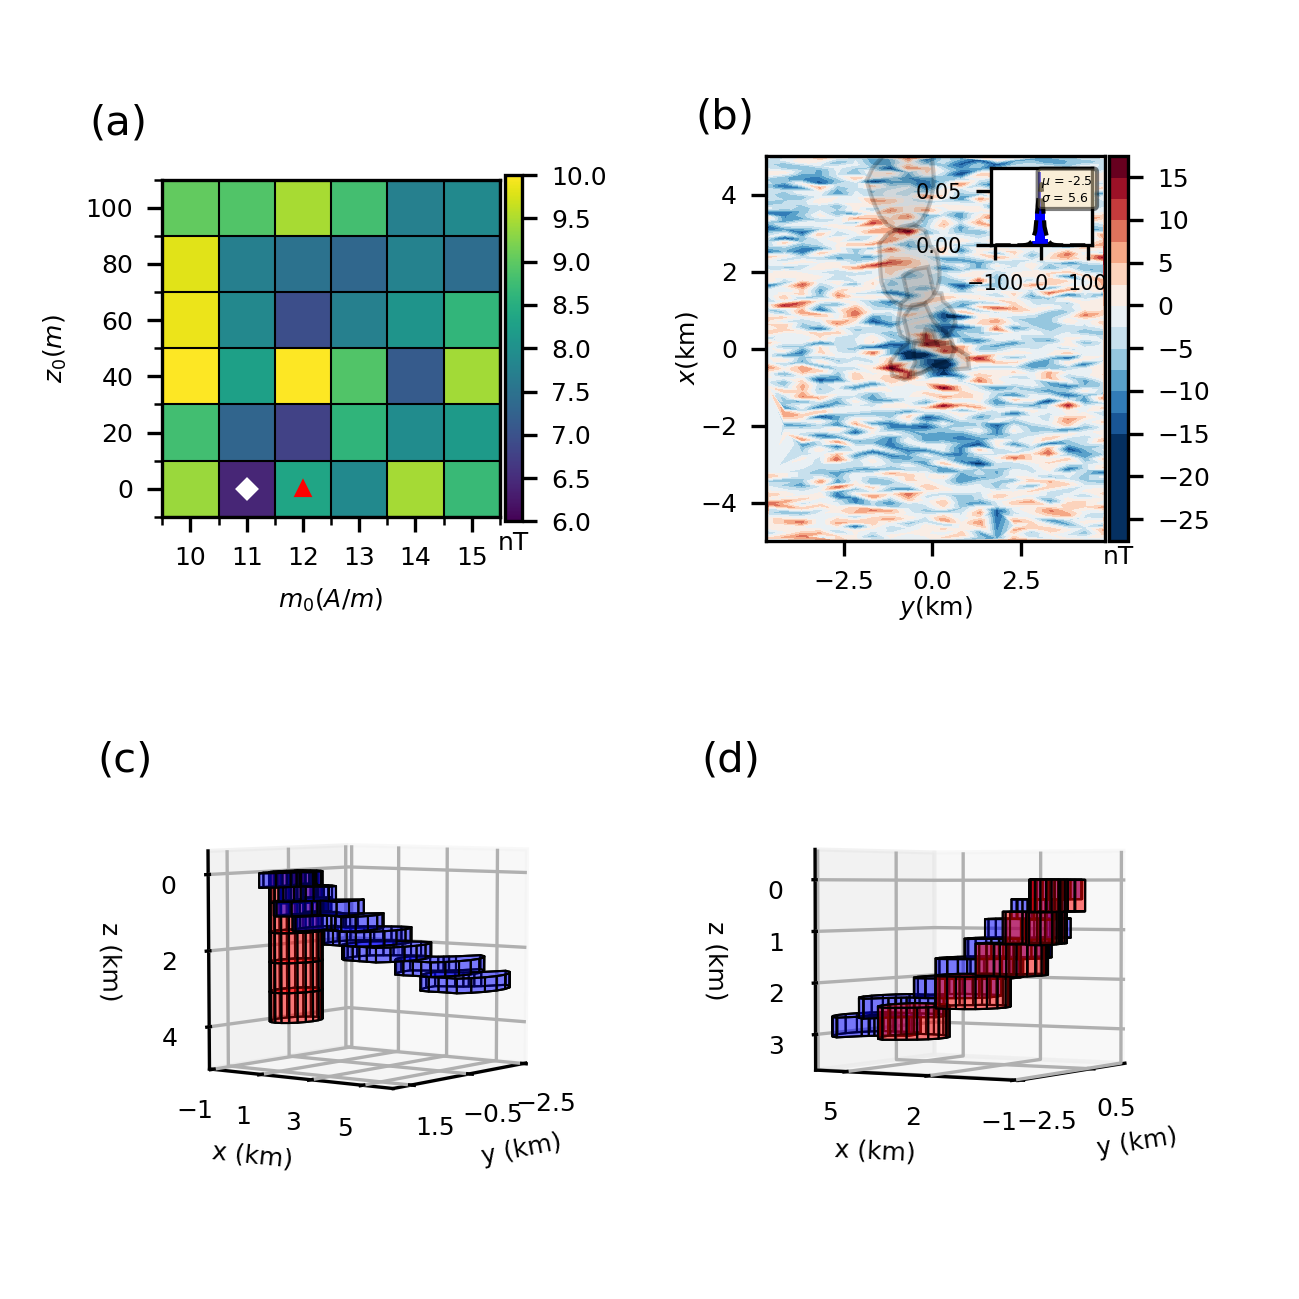
\includegraphics[width=\textwidth]{inclined-l1-solution.png}
	\caption{Soluções L1 obtidas para o modelo inclinado. 
		(a) Mapa discreto da função objetivo produzida pelos modelos da malha de varredura para valores de profundidade do topo $z_{0}$ e intensidade de magnetização total $m_{0}$. 
		O triângulo vermelho representa os valores verdadeiros para $m_{0}$ e $z_{0}$, enquanto o losango branco definem os valores para a melhor solução L1.
		(b) Resíduos entre os dados contaminados com ruído (Figura \ref{fig:inclined_model}a) 
		e os dados preditos (não mostrados) produzidos pela melhor solução L1 (prismas vermelhos no painel d). 
		O histograma dos resíduos inserido em (b) mostra a curva Laplaciana ajustada (linha tracejada).
		Os polígonos cinzas representam as projeções horizontais de todos os prismas que compõe a melhor solução. 
		(c) e (d) Visualização em perspectiva da aproximação inicial (prismas vermelhos) e 
		a melhor solução (prismas vermelhos), respectivamente. Os prismas azuis são o modelo da fonte alvo. 
	}
	\label{fig:inclined_l1_result}
\end{figure}
\pagebreak

\section{Modelo inclinado com regional}

Este teste tem o objetivo de avaliar o desempenho do método em uma situação muito comum em um estudo com dados reais: a presença de um campo regional.
Para simular essa situação, a anomalia de campo total produzida pelo modelo inclinado (Figura \ref{fig:inclined_model}a) foi calculada em uma área maior e somada a um campo regional gerado através de um polinômio de primeira ordem (Fgiuras \ref{fig:great_data}a e \ref{fig:great_data}b).
A partir desses dados, foi estimado um polinômio de primeira ordem por meio do método de mínimos quadrados (Figura \ref{fig:great_data}c) a fim de remover a influência do campo regional da anomalia de campo total (Figura \ref{fig:great_data}d).
Embora a direção do campo regional estimado (Figura \ref{fig:great_data}d) tenha uma direção diferente da verdadeira (Figura \ref{fig:great_data}b), ele recupera muito bem sua amplitude.
A Figura \ref{fig:great_model_rtp}a mostra a anomalia de campo total residual obtida pela remoção do campo regional estimado (Figura \ref{fig:great_data}d) e a Figura \ref{fig:great_model_rtp}b mostra que os resíduos entre a anomalia de campo total residual e a verdadeira (Figuras \ref{fig:great_model_rtp}a e \ref{fig:inclined_model}a) se comportam como ruído, o que indica um bom ajuste dos dados.
O método foi aplicado para inverter a anomalia de campo total residual (Figura \ref{fig:great_model_rtp}a) e obter soluções L2 e L1.
Para cada tipo de solução, foram geradas $36$ soluções L2 e $36$ soluções L1, 
todas elas foram obtidas com a mesma malha de varredura $6 \times 6$ de profundidades do topo $z_{0}$ e intensidade de magnetização total $m_{0}$.
A melhor solução L2 e L1 são definidas como aquelas que produzem o menor valor da função objetivo para cada caso.

A Figura \ref{fig:great_model_rtp}c mostra a anomalia RTP obtida a partir da anomalia de campo total residual (Figura \ref{fig:great_model_rtp}a) e 
a projeção horizontal das aproximações iniciais $\hat{\mathbf{p}}_{(0)}$ 
usadas nas sucessivas inversões (Figuras \ref{fig:great_l2_result} e 
\ref{fig:great_l1_result}).
As aproximações iniciais são compostas de $ L= 5$ prismas com $ V = 20 $ vértices, mesma direção de magnetização do corpo verdadeiro, espessura $ dz=350 $ m e centro em $ (x_0, y_0) = (-200, 0) $.
A Figura \ref{fig:great_l2_result}a mostra que a melhor solução L2 obtida superestima tanto a profundidade do topo $z_{0}$ quanto o valor da intensidade de magnetização total $m_{0}$ verdadeira. Essa solução L2 produz um bom ajuste dos dados (Figura \ref{fig:great_l2_result}b), possui uma profundidade da base em $3063,2$ m e também recupera a geometria do corpo verdadeiro (Figura \ref{fig:great_l2_result}d).
A Figura \ref{fig:great_l1_result} mostra um resultado similar em relação a geometria, porém superestima menos os valores de profundidade do topo $z_{0}$ e subestima pouco o valor da intensidade de magnetização total $m_{0}$. A profundidade da base estimada foi de $2655,6$ m que é um pouco inferior à estimada pela solução L2.
Podemos observar que nesse teste ambas as abordagens L2 e L1 foram bem sucedidas em estimar a forma do corpo e recuperam as feições principais da fonte alvo. Entretanto, nesse caso, a Tabela \ref{tab:inc-reg} mostra que a solução L1 foi superior à solução L2 na estimativa de $ z_0 $ e $ m_0 $.
Todas as soluções L2 produzidas neste teste foram obtidas usando o seguinte conjunto de pesos normalizados $\tilde{\alpha}_{\ell}$ (Equação \ref{eq:alphas}): 
$\tilde{\alpha}_{1} = 10^{-3}$, $\tilde{\alpha}_{2} = 10^{-3}$, 
$\tilde{\alpha}_{3} = 10^{-6}$, $\tilde{\alpha}_{4} = 10^{-6}$, e 
$\tilde{\alpha}_{5} = 10^{-5}$. 
Já as soluções L1 foram obtidas utilizando o conjunto: 
$\tilde{\alpha}_{1} = 10^{-4}$, $\tilde{\alpha}_{2} = 10^{-5}$, 
$\tilde{\alpha}_{3} = 10^{-6}$, $\tilde{\alpha}_{4} = 10^{-7}$, e 
$\tilde{\alpha}_{5} = 10^{-4}$.
É importante notar que, mesmo a solução L1 sendo superior à solução L2, não há diferenças significativas entre as soluções L2 e L1 obtidas pelo método.

\begin{table}[h]\label{tab:inc-reg}
	\caption{Valores dos vínculos na iteração final para as melhores soluções L2 e L1 da aplicação ao corpo complexo na presença de uma fonte não-alvo pequena (Eqs. \ref{eq:phi1}, \ref{eq:phi2}, \ref{eq:phi3}, \ref{eq:phi4} e \ref{eq:phi5}).}
	\centering
	\vspace{0.5cm}
	\begin{tabular}{c|ccccc}
		Vínculo & $ \varphi _1 $ & $ \varphi _2 $ &  $ \varphi _3 $ &  $ \varphi _4 $ &  $ \varphi _5 $ \\
		\hline
		Solução L2 & $ 6,05 $ & $ 16,32 $ & $ 0,15 $ & $0,28 $ & $ 0,75 $ \\ 
		Solução L1 & $ 0,79 $ & $ 0,22 $ & $ 0,10 $ & $0,02$ & $ 3,38$
	\end{tabular}
\end{table}

\begin{figure}[!htb]
	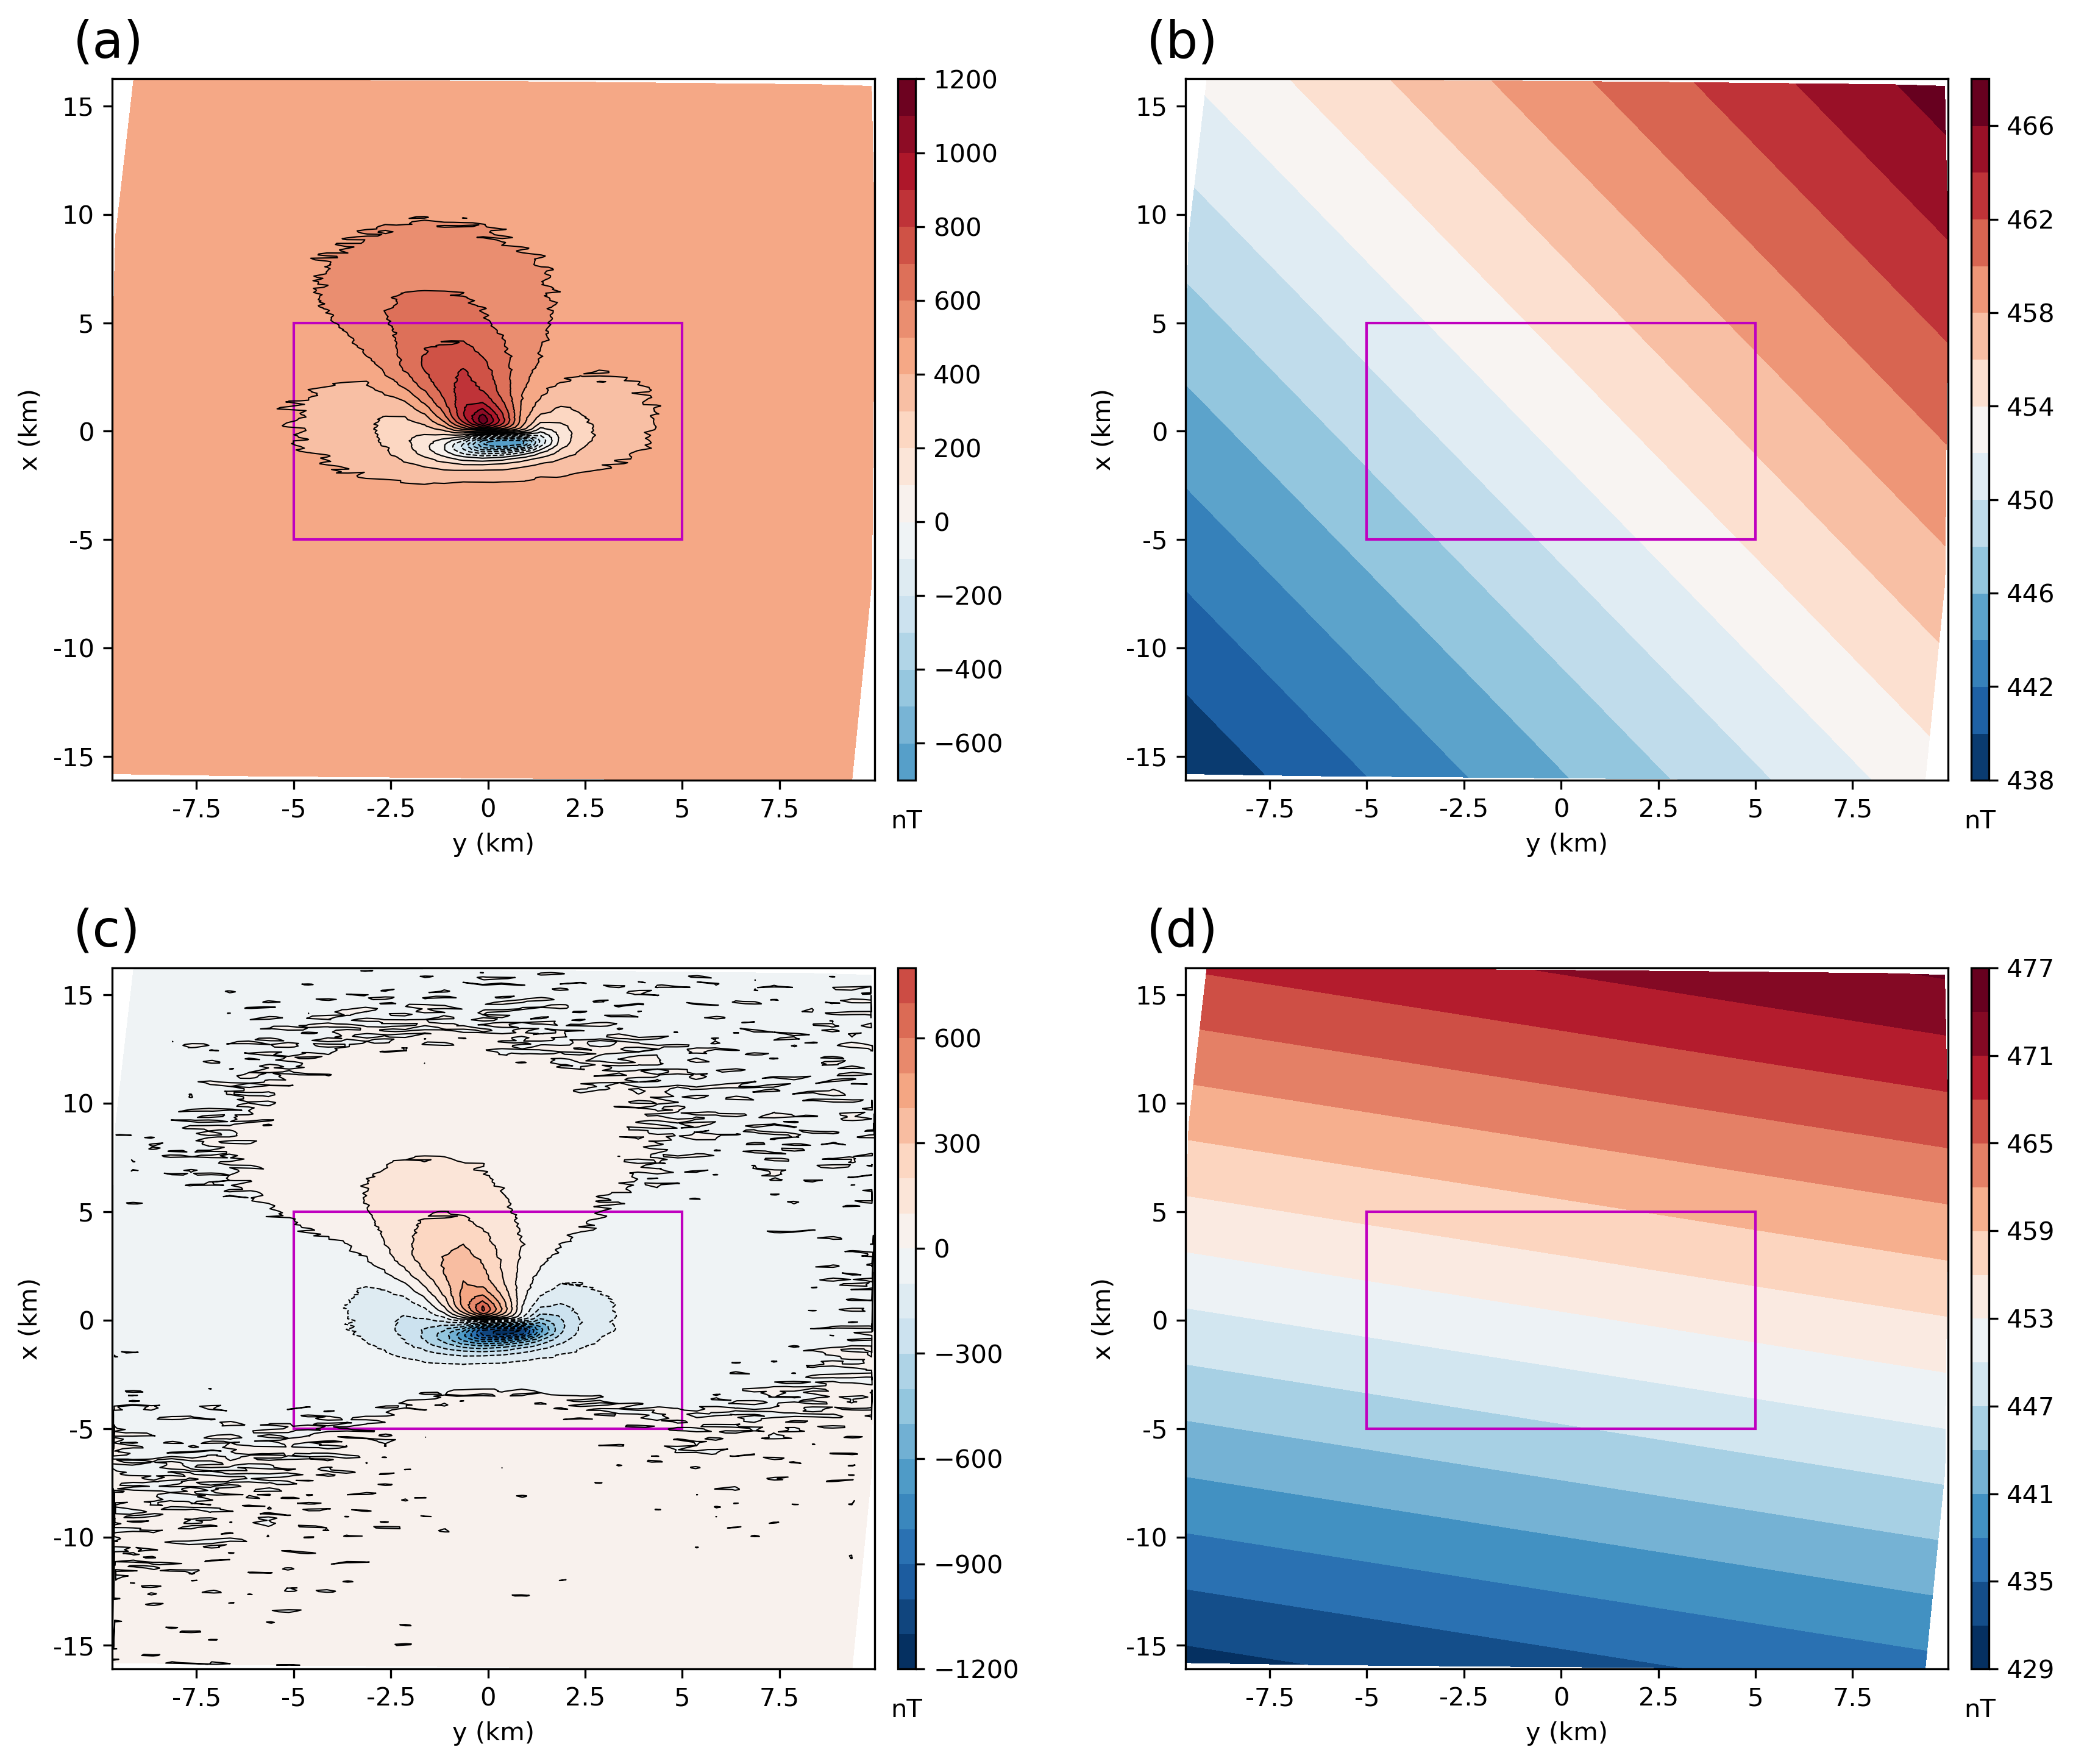
\includegraphics[width=\textwidth]{inclined-data-large.png}
	\caption{Aplicação aos dados do modelo inclinado com regional. 
		(a) Anomalia de campo total produzida pela modelo inclinado (Figura \ref{fig:inclined_model}a) somada a um campo regional sintético (painel b).
		(b) Polinômio de primeira ordem que representa o campo regional sintético.
		(c) Anomalia de campo total residual obtida pela diferença entre (a) e (d). (d) Campo regional estimado por um polinômio simples através de mínimos quadrados.
	}
	\label{fig:great_data}
\end{figure}
\pagebreak

\pagebreak

\begin{figure}[!htb]
	\centering
	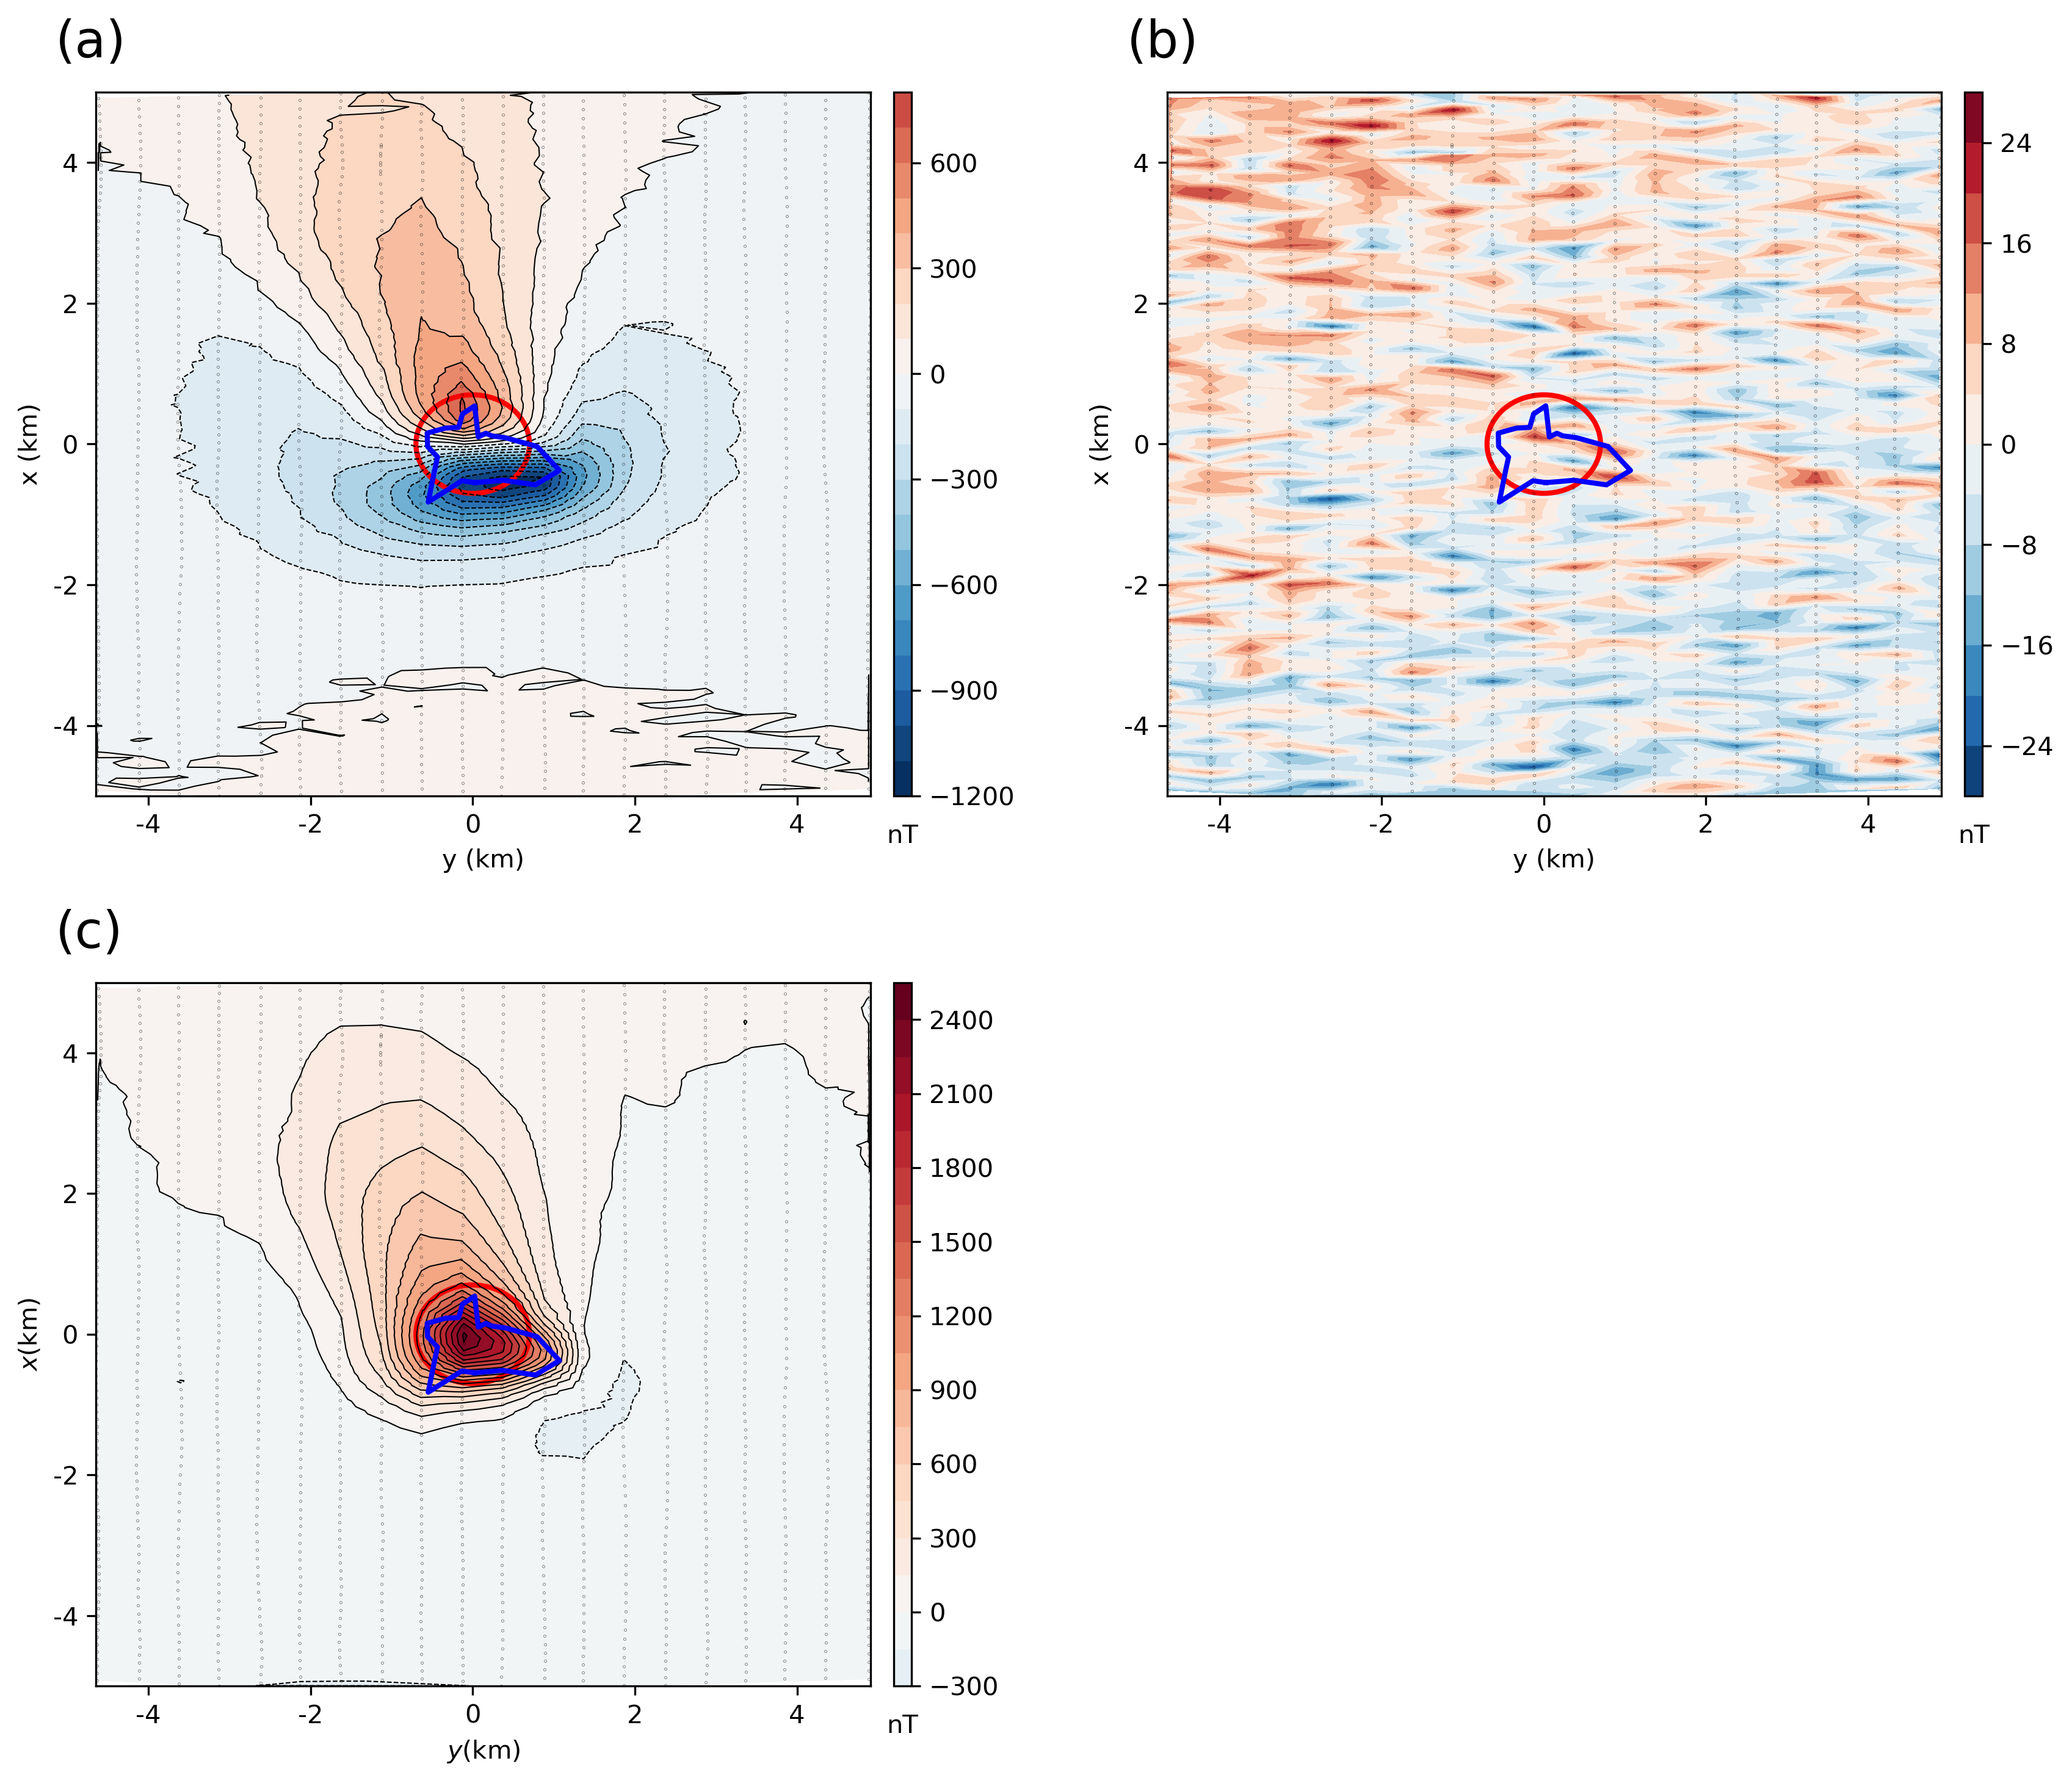
\includegraphics[width=\textwidth]{great_rtp.png}
	\caption{Aplicação aos dados do modelo inclinado com regional. 
		(a) Anomalia de campo total residual contida no retângulo rosa na Figura \ref{fig:great_data}c. (b) Resíduos obtidos pela diferença entre as anomalias de campo total gerada no teste anterior (Figrura \ref{fig:inclined_model}a) e a residual (painel a). (c) Anomalia RTP sobre a área de estudo. Ambos painéis são limitados pelo retângulos rosa na Figura \ref{fig:great_data}. As linhas azuis e vermelhas correspondem, respectivamente, às projeções horizontais da porção mais rasa da fonte alvo e da aproximação inicial utilizada nas inversões subsequentes (prismas vermelhos nas Figuras \ref{fig:great_l2_result}c e 
		\ref{fig:great_l1_result}c).
	}
	\label{fig:great_model_rtp}
\end{figure}

\pagebreak

\begin{figure}[!htb]
	\centering
	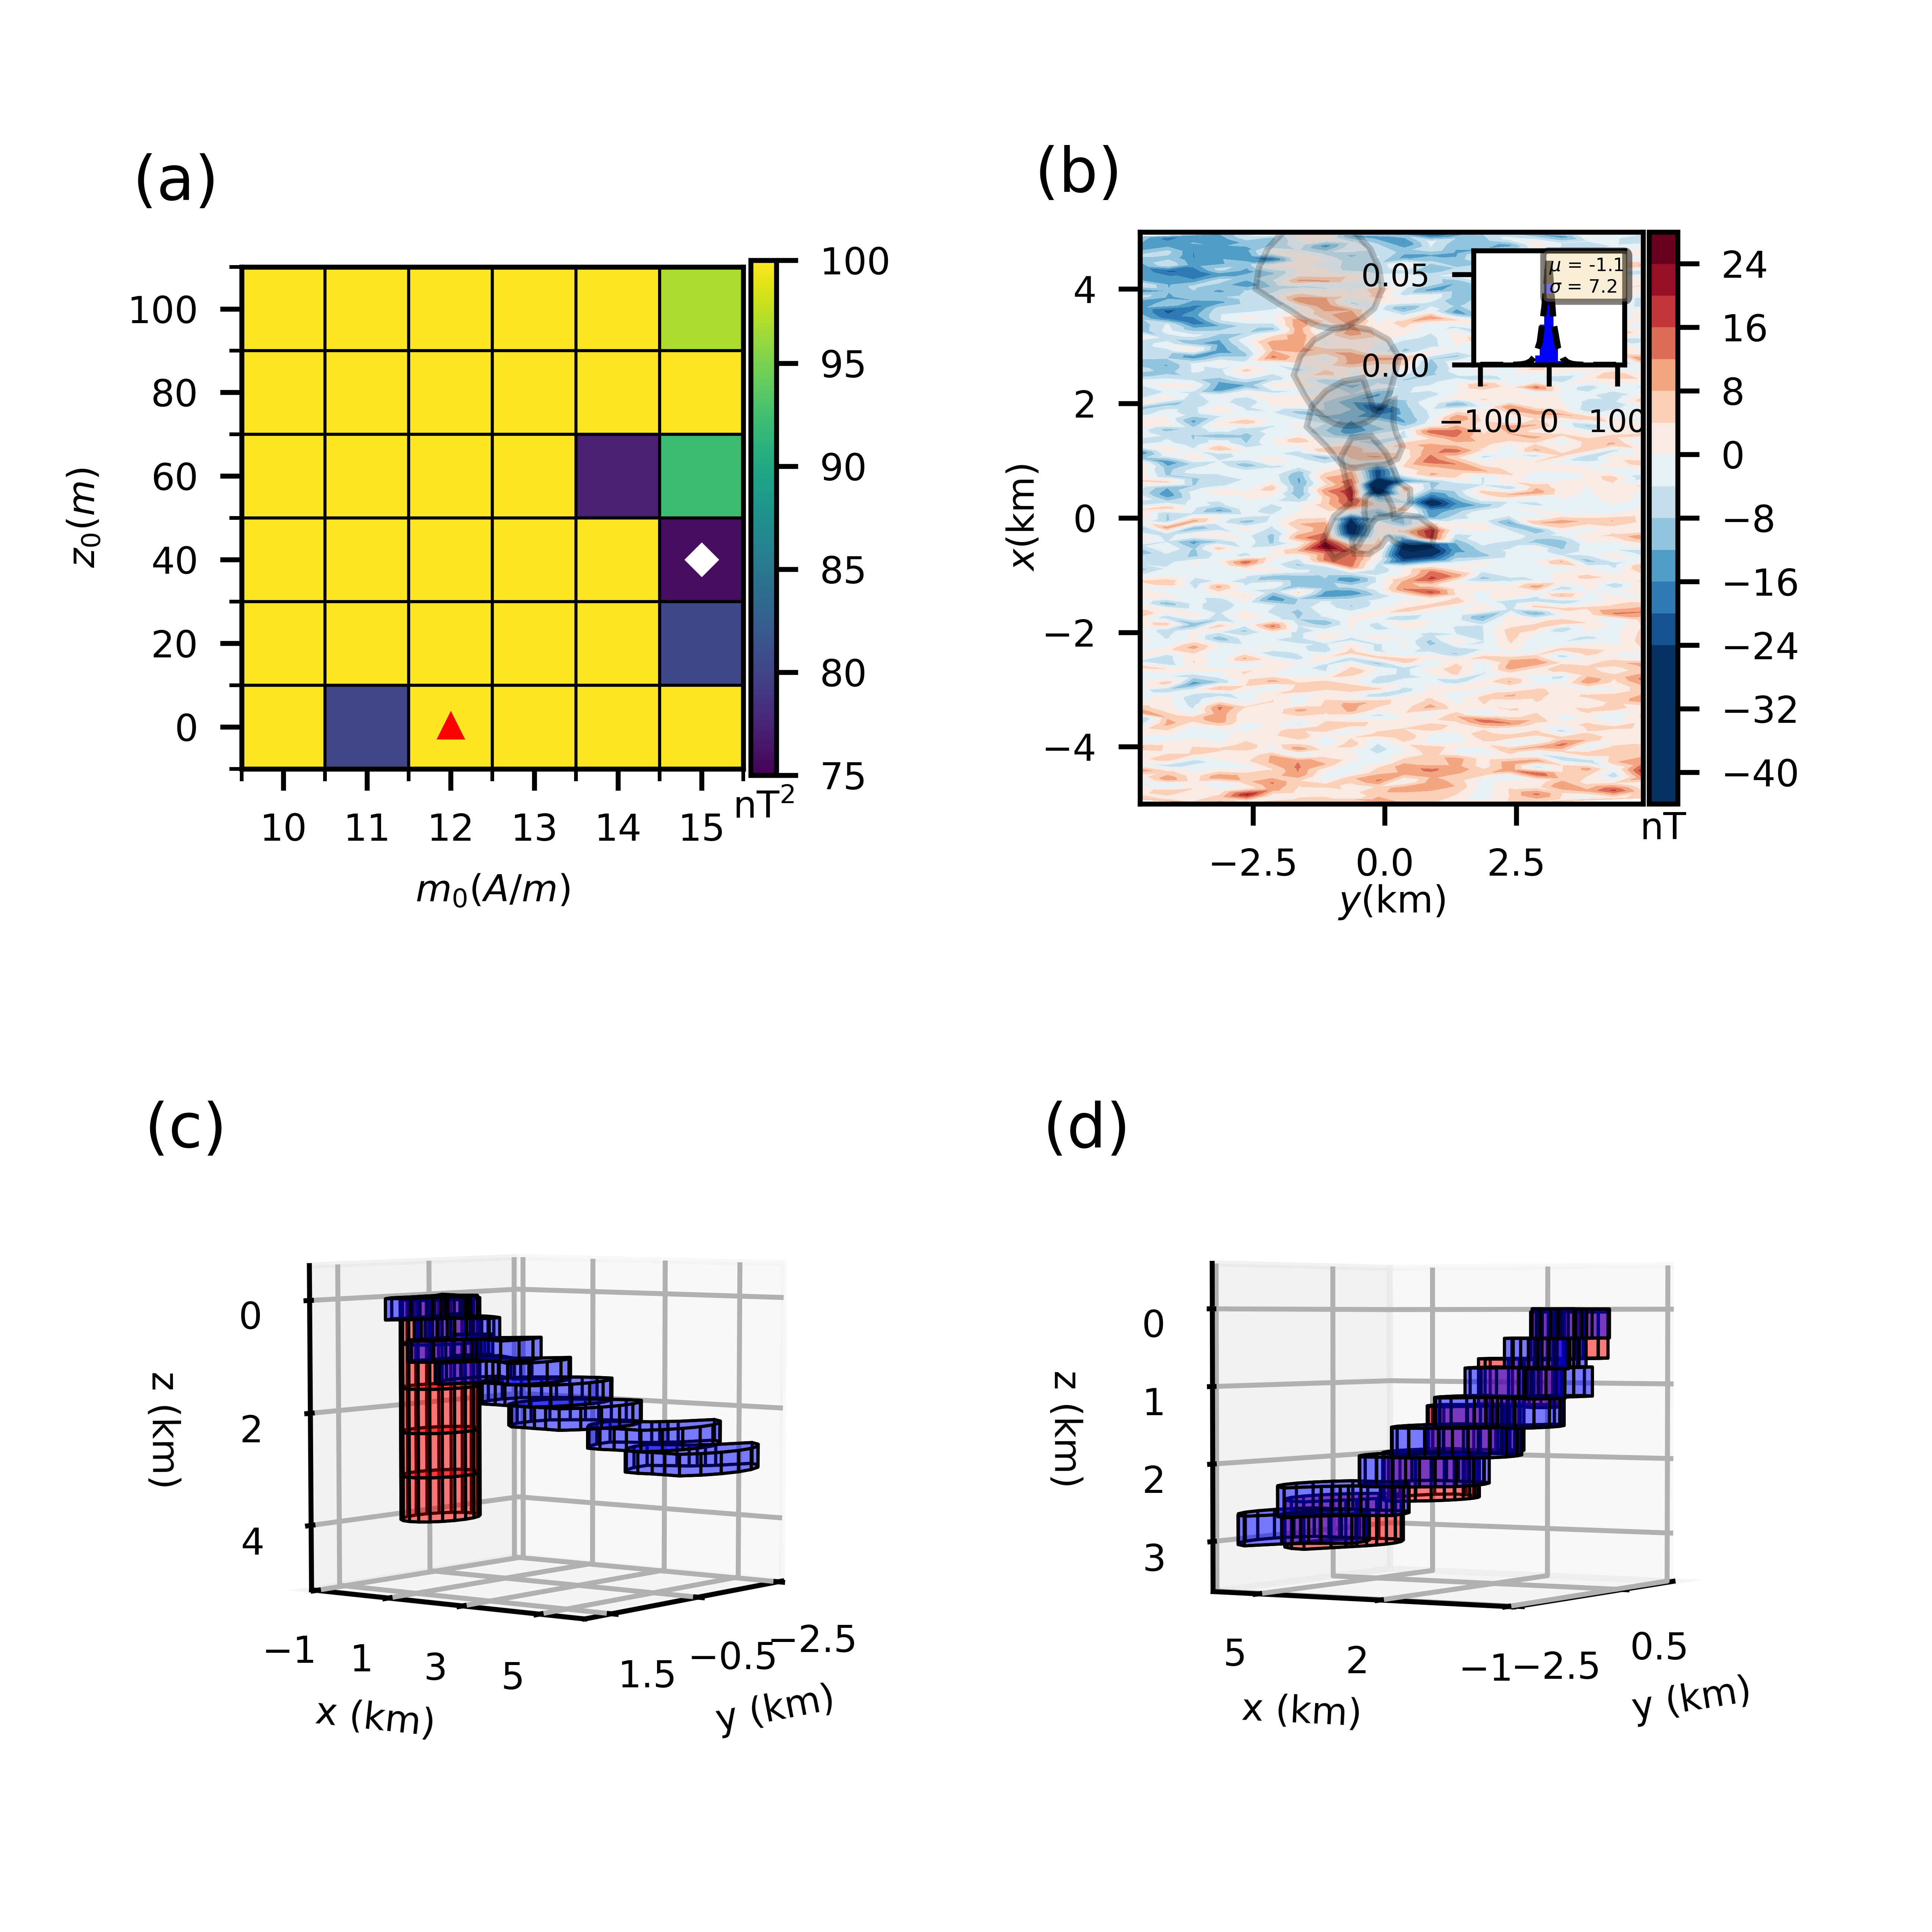
\includegraphics[width=\textwidth]{great-l2-solution.png}
	\caption{Soluções L2 obtidas para o modelo inclinado com regional. 
		(a) Mapa discreto da função objetivo produzida pelos modelos obtidos a partir da varredura de valores de profundidade do topo $z_{0}$ e intensidade de magnetização total $m_{0}$. 
		O triângulo vermelho representa os valores verdadeiros para $m_{0}$ e $z_{0}$ eo losango branco indica os valores que definem a melhor solução L2.
		(b) Resíduos entre a anomalia de campo total residual (Figura \ref{fig:great_model_rtp}a) 
		e os dados preditos (não mostrados) produzidos pela melhor solução L2 (prismas vermelhos no painel d). 
		O histograma dos resíduos inserido em (b) mostra a curva Gaussiana ajustada (linha tracejada).
		Os polígonos cinzas representam as projeções horizontais de todos os prismas que compõe a melhor solução. 
		(c) e (d) Visualização em perspectiva da aproximação inicial (prismas vermelhos) e 
		a melhor solução (prismas vermelhos), respectivamente. Os prismas azuis são o modelo da fonte alvo. 
	}
	\label{fig:great_l2_result}
\end{figure}
\pagebreak
\begin{figure}[!htb]
	\centering
	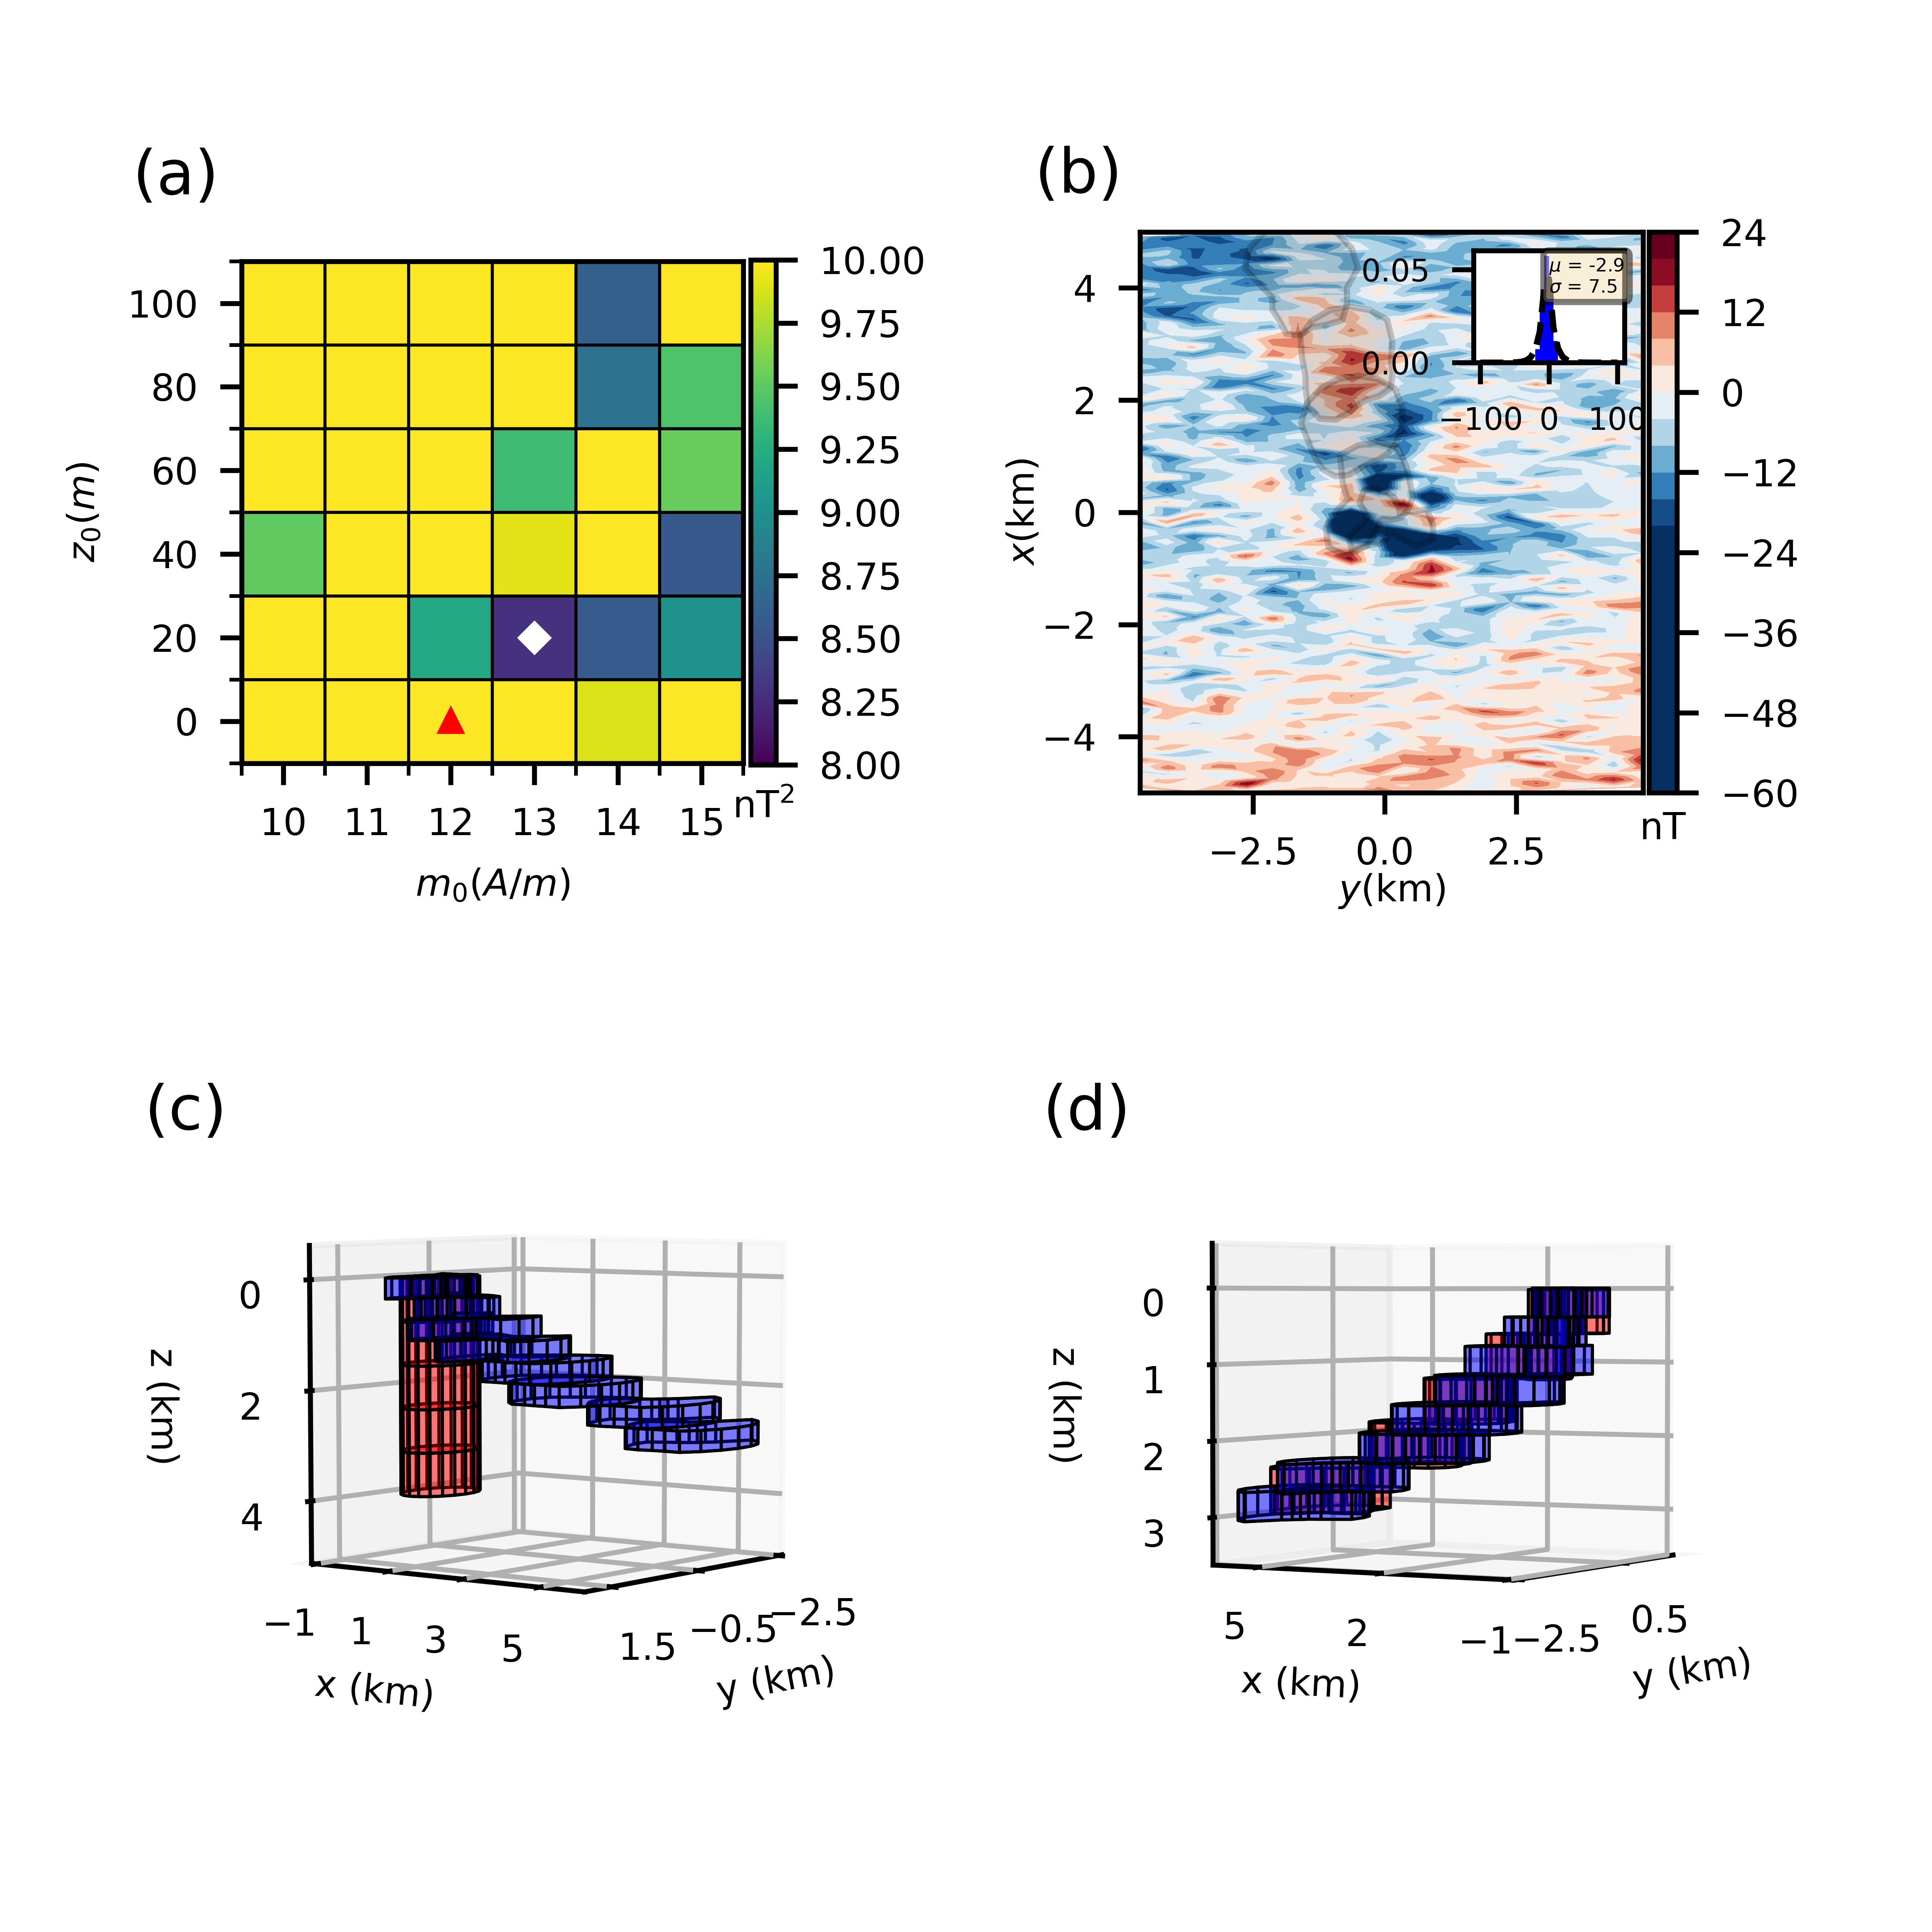
\includegraphics[width=\textwidth]{great-l1-solution.png}
	\caption{Soluções L1 obtidas para o modelo inclinado com regional. 
		(a) Mapa discreto da função objetivo produzida pelos modelos da malha de varredura para valores de profundidade do topo $z_{0}$ e intensidade de magnetização total $m_{0}$. 
		O triângulo vermelho representa os valores verdadeiros para $m_{0}$ e $z_{0}$ e o losango branco indica os valores que definem a melhor solução L1.
		(b) Resíduos entre a anomalia de campo total residual (Figura \ref{fig:great_model_rtp}a) 
		e os dados preditos (não mostrados) produzidos pela melhor solução L1 (prismas vermelhos no painel d). 
		O histograma dos resíduos inserido em (b) mostra a curva Laplaciana ajustada (linha tracejada).
		Os polígonos cinzas representam as projeções horizontais de todos os prismas que compõe a melhor solução. 
		(c) e (d) Visualização em perspectiva da aproximação inicial (prismas vermelhos) e 
		a melhor solução (prismas vermelhos), respectivamente. Os prismas azuis são o modelo da fonte alvo. 
	}
	\label{fig:great_l1_result}
\end{figure}
\pagebreak


\section{Modelo complexo}
\label{sec:target_source_without_interference}

Com o propósito de aplicar o método a problemas mais realistas, foi simulado um corpo geológico complexo imerso em meio não magnético (prismas azuis nas Figuras 
\ref{fig:target_model}, \ref{fig:target_l2_result}, \ref{fig:target_l1_result},
\ref{fig:small_model}, \ref{fig:small_l2_result}, \ref{fig:small_l1_result}, 
\ref{fig:thick_model}, \ref{fig:thick_l2_result}, e \ref{fig:thick_l1_result})
que representa a fonte alvo 3D com profundidade do topo em $130$ m, profundidade da base em $6130$ m, centro em $ (x_0, y_0) = (-250, 250) $ e um vetor de magnetização total constante com inclinação $-50^{\circ}$, 
declinação $9^{\circ}$, e intensidade $12$ A/m. 
Esse modelo é composto de $ 10 $ prismas verticalmente justapostos com um deslocamento horizontal entre eles, que simula uma intrusão em forma de dique, e mergulho de alto ângulo para NO.
Recuperar a geometria desse corpo simulado é uma tarefa complicada porque ele possui um mergulho NO-SE e suas fatias horizontais mostram uma forma que varia ao longo da profundidade, assim, é possível notar que o corpo não satisfaz perfeitamente os vínculos impostos nesse método.
A violação dos vínculos pode ser visualizada pela falta de suavidade entre os raios adjacentes que definem a seção horizontal de cada prisma e entre os raios adjacentes entre prismas verticalmente adjacentes.
A anomalia de campo total (Figura \ref{fig:target_model}a) produzida pela fonte alvo foi calculada em $1939$ pontos localizados sobre uma superfície ondulada que simula um levantamento aéreo (Figura \ref{fig:target_model}b). Esses dados sintéticos foram contaminados com um ruído Gaussiano pseudo-aleatório de média zero e desvio padrão igual a $5$ nT.
O método foi aplicado para inverter esse dado contaminado com ruído e obter soluções L2 e L1 para três cenários: sem fontes não-alvo, 
com uma fonte não-alvo relativamente pequena e com uma fonte não-alvo relativamente grande.
Para cada cenário, foram geradas $36$ soluções L2 e $36$ soluções L1, 
todas elas foram obtidas com a mesma malha de varredura $6 \times 6$ de profundidades do topo $z_{0}$ e intensidade de magnetização total $m_{0}$.
A melhor solução L2 e L1 são definidas como aquelas que produzem o menor valor da função objetivo para cada caso.

A Figura \ref{fig:target_model_rtp} mostra a anomalia RTP obtida a partir da anomalia de campo total contaminada com ruído (Figura \ref{fig:target_model}a) e 
a projeção horizontal das aproximações iniciais $\hat{\mathbf{p}}_{(0)}$ 
usadas nas sucessivas inversões (Figuras \ref{fig:target_l2_result} e 
\ref{fig:target_l1_result}).
As aproximações iniciais são compostas de $ L= 10$ prismas com $ V = 20 $ vértices, mesma direção de magnetização do corpo verdadeiro, espessura $ dz=650 $ m e centro em $ (x_0, y_0) = (-300, 300) $.
A Figura \ref{fig:target_l2_result}a mostra que a melhor solução L2 foi obtida através dos valores verdadeiros da profundidade do topo $z_{0}$ e intensidade de magnetização total $m_{0}$. Essa solução L2 produz um ótimo ajuste dos dados (Figura \ref{fig:target_l2_result}b), possui uma profundidade da base em $6663,8$ m e também recupera a geometria do corpo verdadeiro (Figura \ref{fig:target_l2_result}d).
A Figura \ref{fig:target_l1_result} mostra um resultado similar produzido pela melhor solução L1, que tem profundidade da base em $6703,0$ m.
O aspecto mais interessante das soluções L2 e L1 obtidas neste teste é que elas recuperam não só as feições principais da fonte mas também seu mergulho e a variação de sua forma ao longo da profundidade.
Todas as soluções L2 e L1 produzidas neste teste foram obtidas usando o seguinte conjunto de pesos normalizados $\tilde{\alpha}_{\ell}$ (Equação \ref{eq:alphas}): 
$\tilde{\alpha}_{1} = 10^{-5}$, $\tilde{\alpha}_{2} = 10^{-4}$, 
$\tilde{\alpha}_{3} = 10^{-4}$, $\tilde{\alpha}_{4} = 10^{-8}$, e 
$\tilde{\alpha}_{5} = 10^{-6}$. 
Segundo a Tabela \ref{tab:complex}, a solução L1 é ligeiramente superior à solução L2, porém os valores dos vínculos para cada solução são muito próximos.
É importante notar que, devido à ausência de fontes não-alvo neste teste, não há diferenças práticas entre as soluções L2 e L1 obtidas pelo método aqui proposto.


\begin{table}[h]\label{tab:complex}
	\caption{Valores dos vínculos na iteração final para as melhores soluções L2 e L1 da aplicação ao corpo complexo na presença de uma fonte não-alvo pequena (Eqs. \ref{eq:phi1}, \ref{eq:phi2}, \ref{eq:phi3}, \ref{eq:phi4} e \ref{eq:phi5}).}
	\centering
	\vspace{0.5cm}
	\begin{tabular}{c|ccccc}
		Vínculo & $ \varphi _1 $ & $ \varphi _2 $ &  $ \varphi _3 $ &  $ \varphi _4 $ &  $ \varphi _5 $ \\
		\hline
		Solução L2 & $ 0,39 $ & $ 4,05 $ & $ 0,86 $ & $1,80 \times 10^{-2} $ & $ 0,60 $ \\ 
		Solução L1 & $ 0,26 $ & $ 2,18 $ & $ 0,85 $ & $1,81 \times 10^{-2} $ & $ 0,61 $
	\end{tabular}
\end{table}


\begin{figure}[!htb]
	\centering
	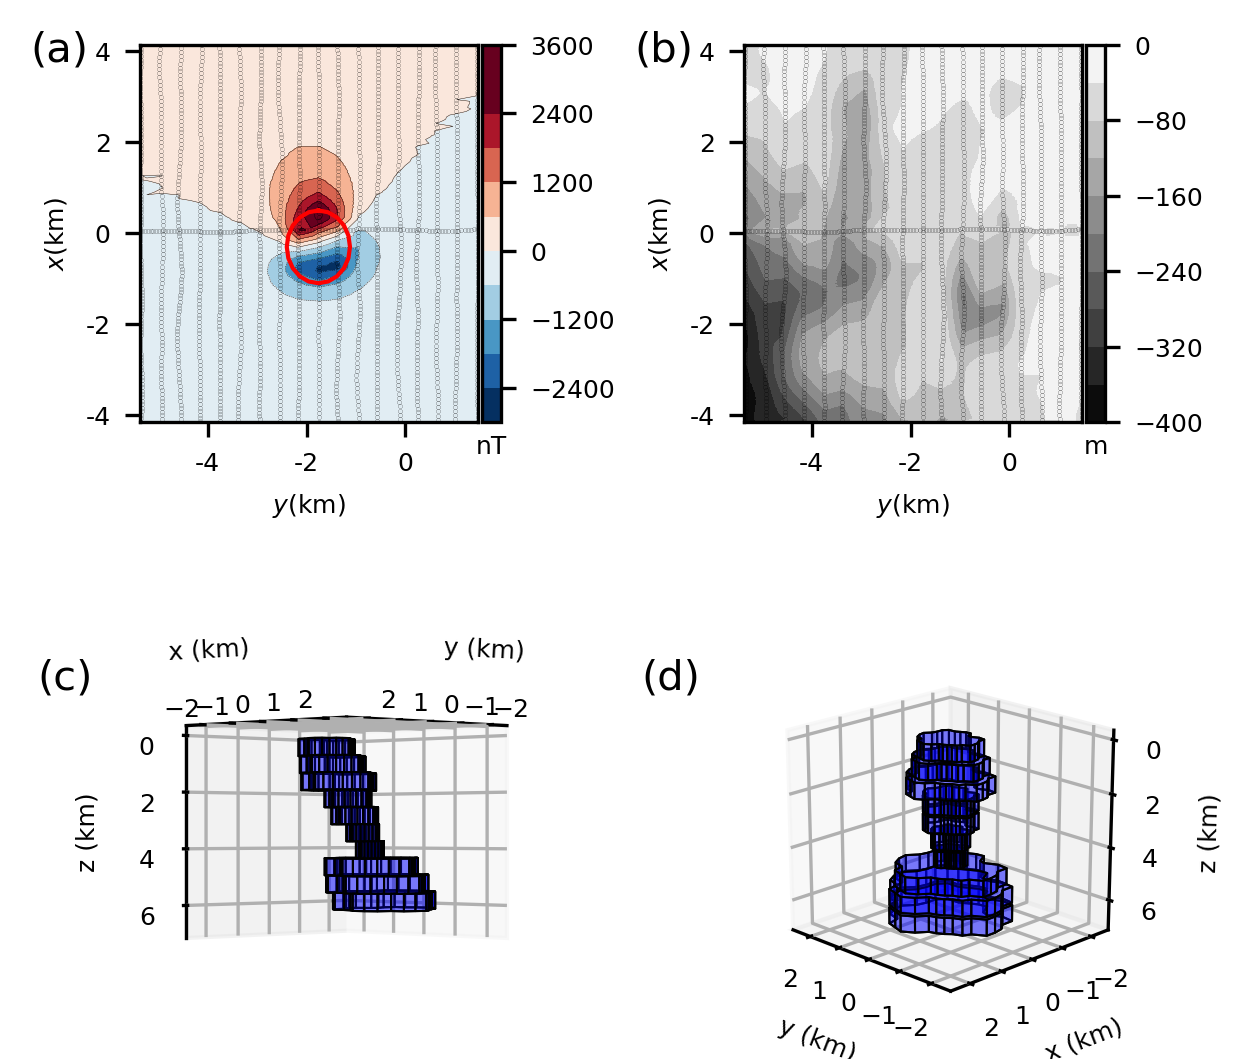
\includegraphics[width=\textwidth]{complex_model_data.png}
	\caption{Modelo da fonte alvo. (a) Anomalia de campo total contaminada com ruído produzida pela fonte alvo (prismas azuis mostrados nos painéis c e d). Os pontos pretos representam os pontos de observação. O círculo vermelho representa a projeção horizontal da aproximação inicial $\hat{\mathbf{p}}_{(0)}$ (prismas vermelhos nas Figuras
		\ref{fig:target_l2_result}c e \ref{fig:target_l1_result}c). (b) Coordenadas verticais dos pontos de observação que simulam um levantamento aéreo.
		(c) e (d) Visualizações em perspectiva do modelo da fonte alvo representada pelos prismas azuis.
	}
	\label{fig:target_model}
\end{figure}
\pagebreak

\begin{figure}[!htb]
	\centering
	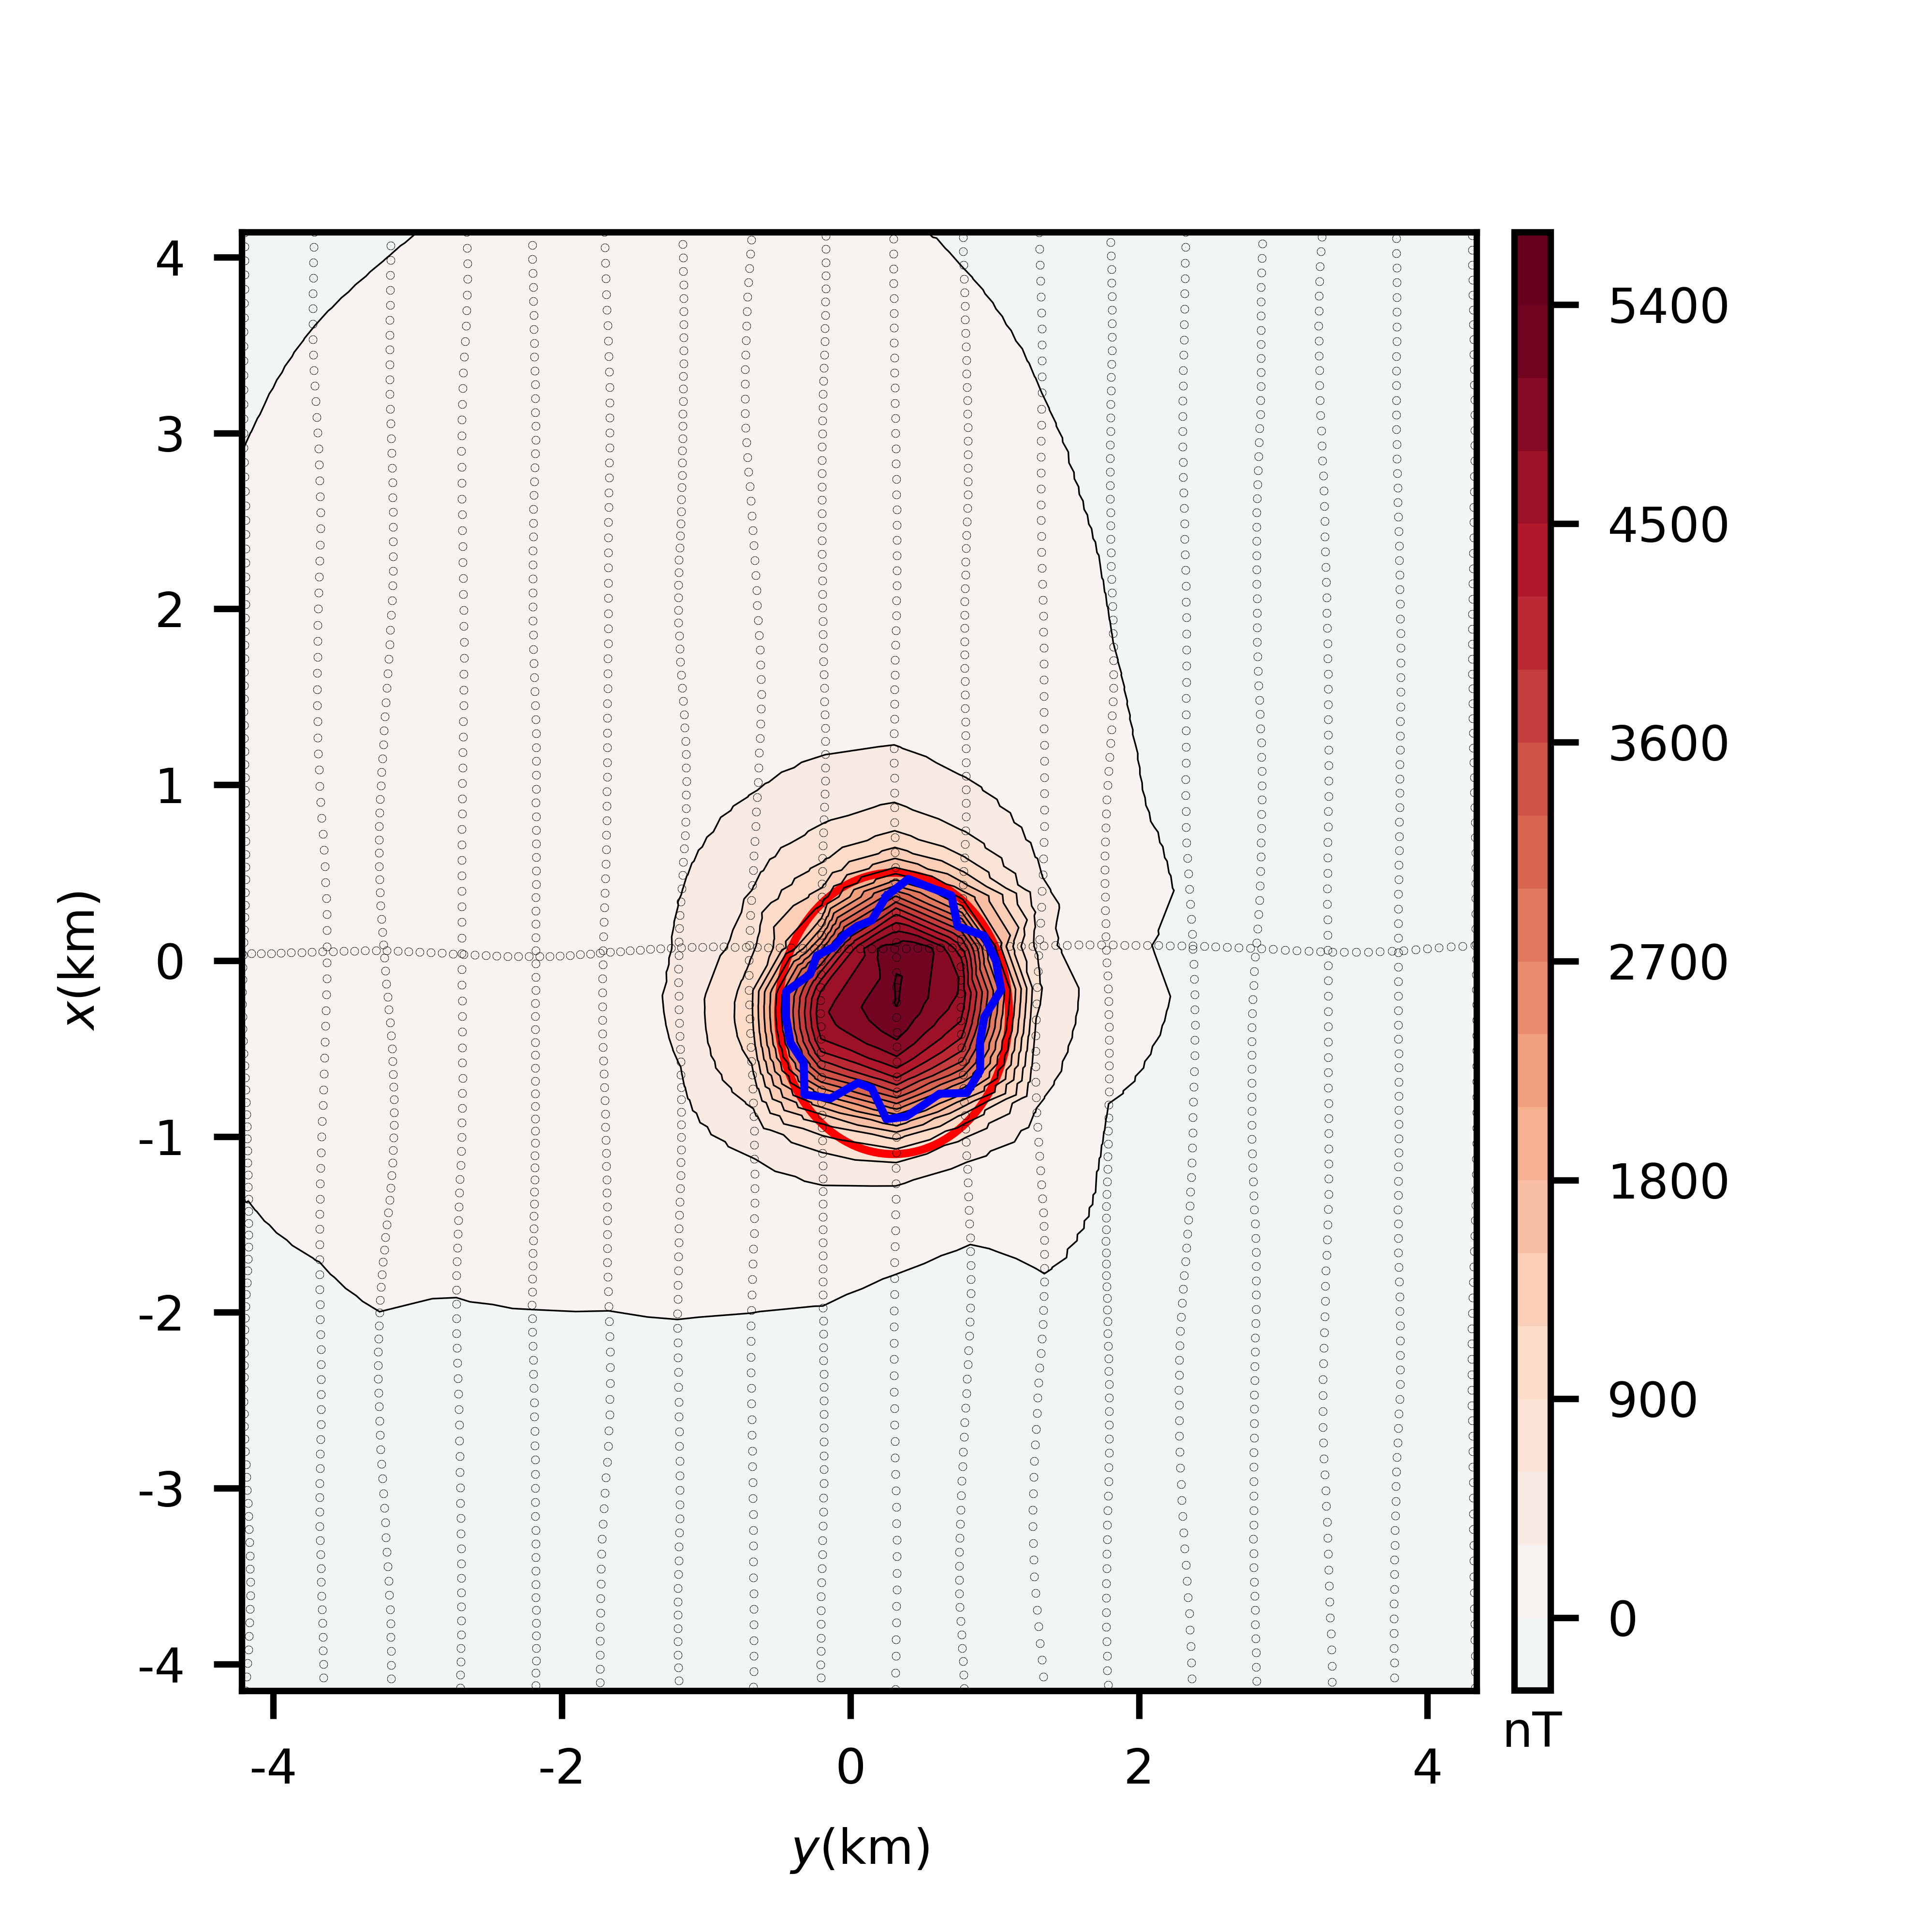
\includegraphics[width=\textwidth]{complex_rtp.png}
	\caption{Anomalia RTP produzida pela fonte alvo. 
		A anomalia RTP mostra valores predominantemente positivos logo acima da fonte alvo. Os pontos pretos representam os pontos de observação. As linhas azuis e vermelhas correspondem, respectivamente, às projeções horizontais da porção mais rasa da fonte alvo e da aproximação inicial utilizada nas inversões subsequentes (prismas vermelhos nas Figuras \ref{fig:target_l2_result}c e 
		\ref{fig:target_l1_result}c).
	}
	\label{fig:target_model_rtp}
\end{figure}

\pagebreak

\begin{figure}[!htb]
	\centering
	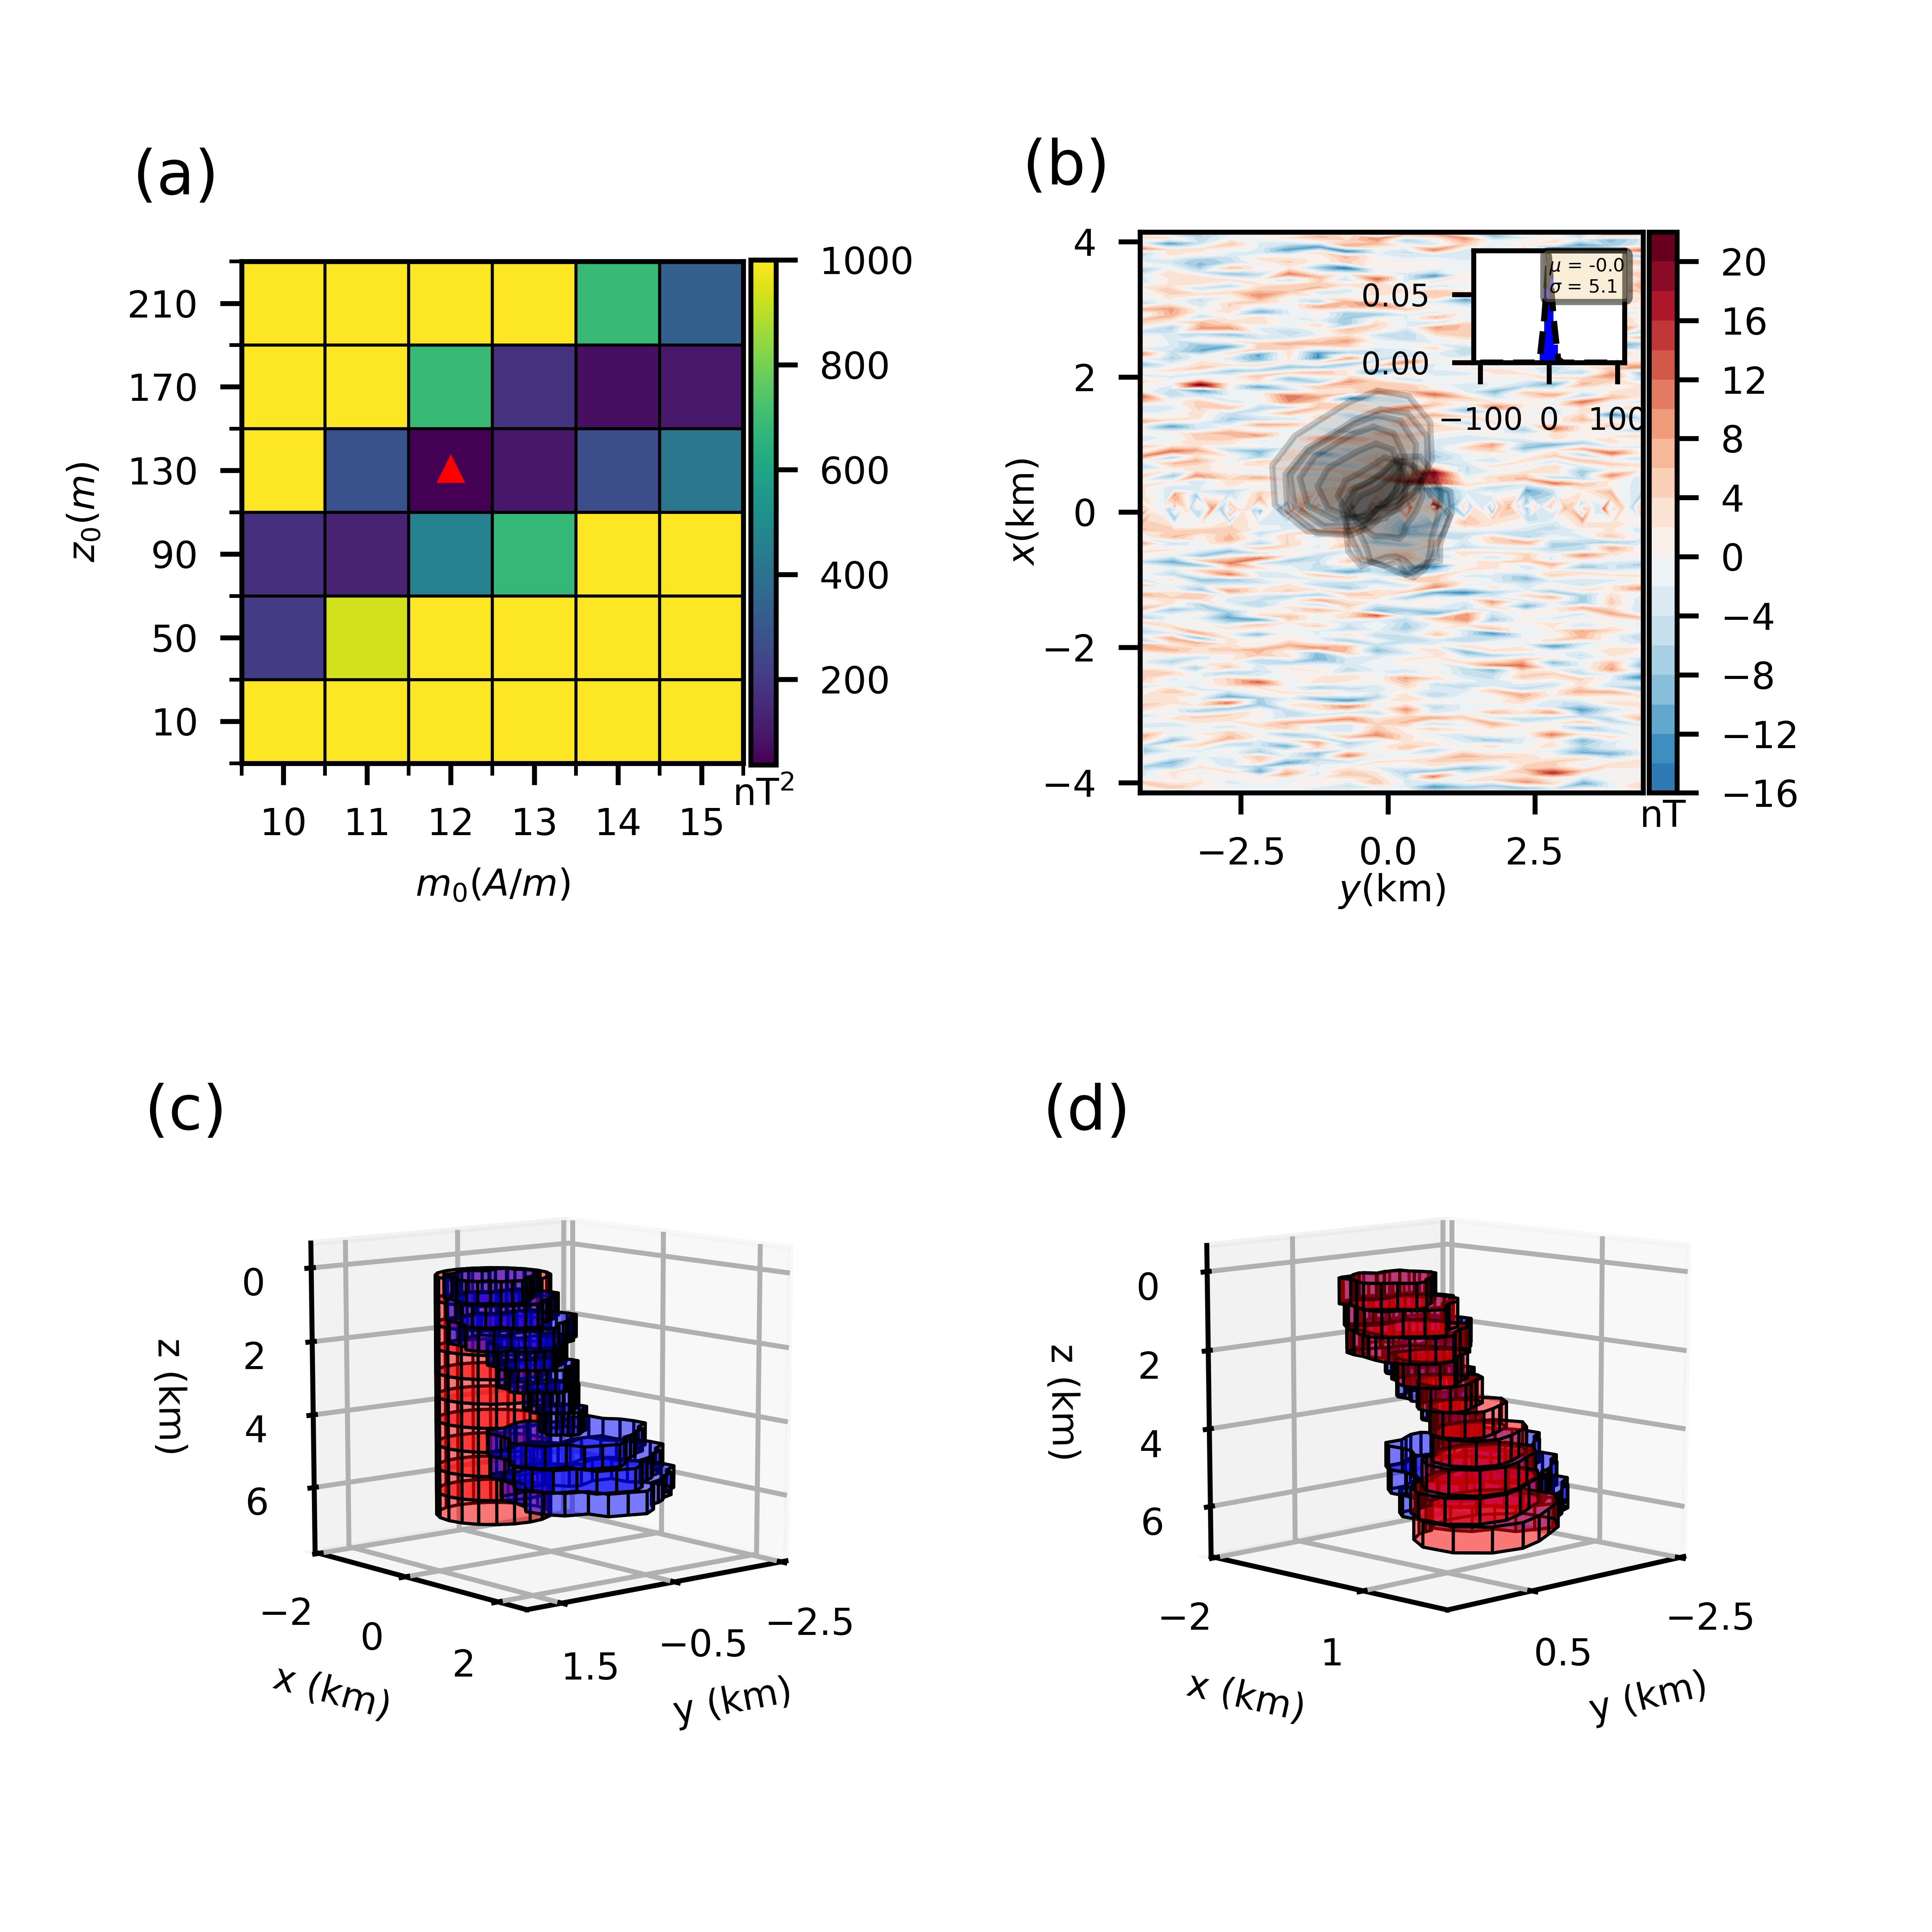
\includegraphics[width=\textwidth]{complex-l2-solution.png}
	\caption{Soluções L2 obtidas para o modelo da fonte alvo sem interferência. 
		(a) Mapa discreto da função objetivo produzida pelos modelos obtidos a partir da varredura de valores de profundidade do topo $z_{0}$ e intensidade de magnetização total $m_{0}$. 
		O triângulo vermelho representa os valores verdadeiros para $m_{0}$ e $z_{0}$, assim como os valores que definem a melhor solução L2.
		(b) Resíduos entre os dados contaminados com ruído (Figura \ref{fig:target_model}a) 
		e os dados preditos (não mostrados) produzidos pela melhor solução L2 (prismas vermelhos no painel d). 
		O histograma dos resíduos inserido em (b) mostra a curva Gaussiana ajustada (linha tracejada).
		Os polígonos cinzas representam as projeções horizontais de todos os prismas que compõe a melhor solução. 
		(c) e (d) Visualização em perspectiva da aproximação inicial (prismas vermelhos) e 
		a melhor solução (prismas vermelhos), respectivamente. Os prismas azuis são o modelo da fonte alvo. 
	}
	\label{fig:target_l2_result}
\end{figure}
\pagebreak
\begin{figure}[!htb]
	\centering
	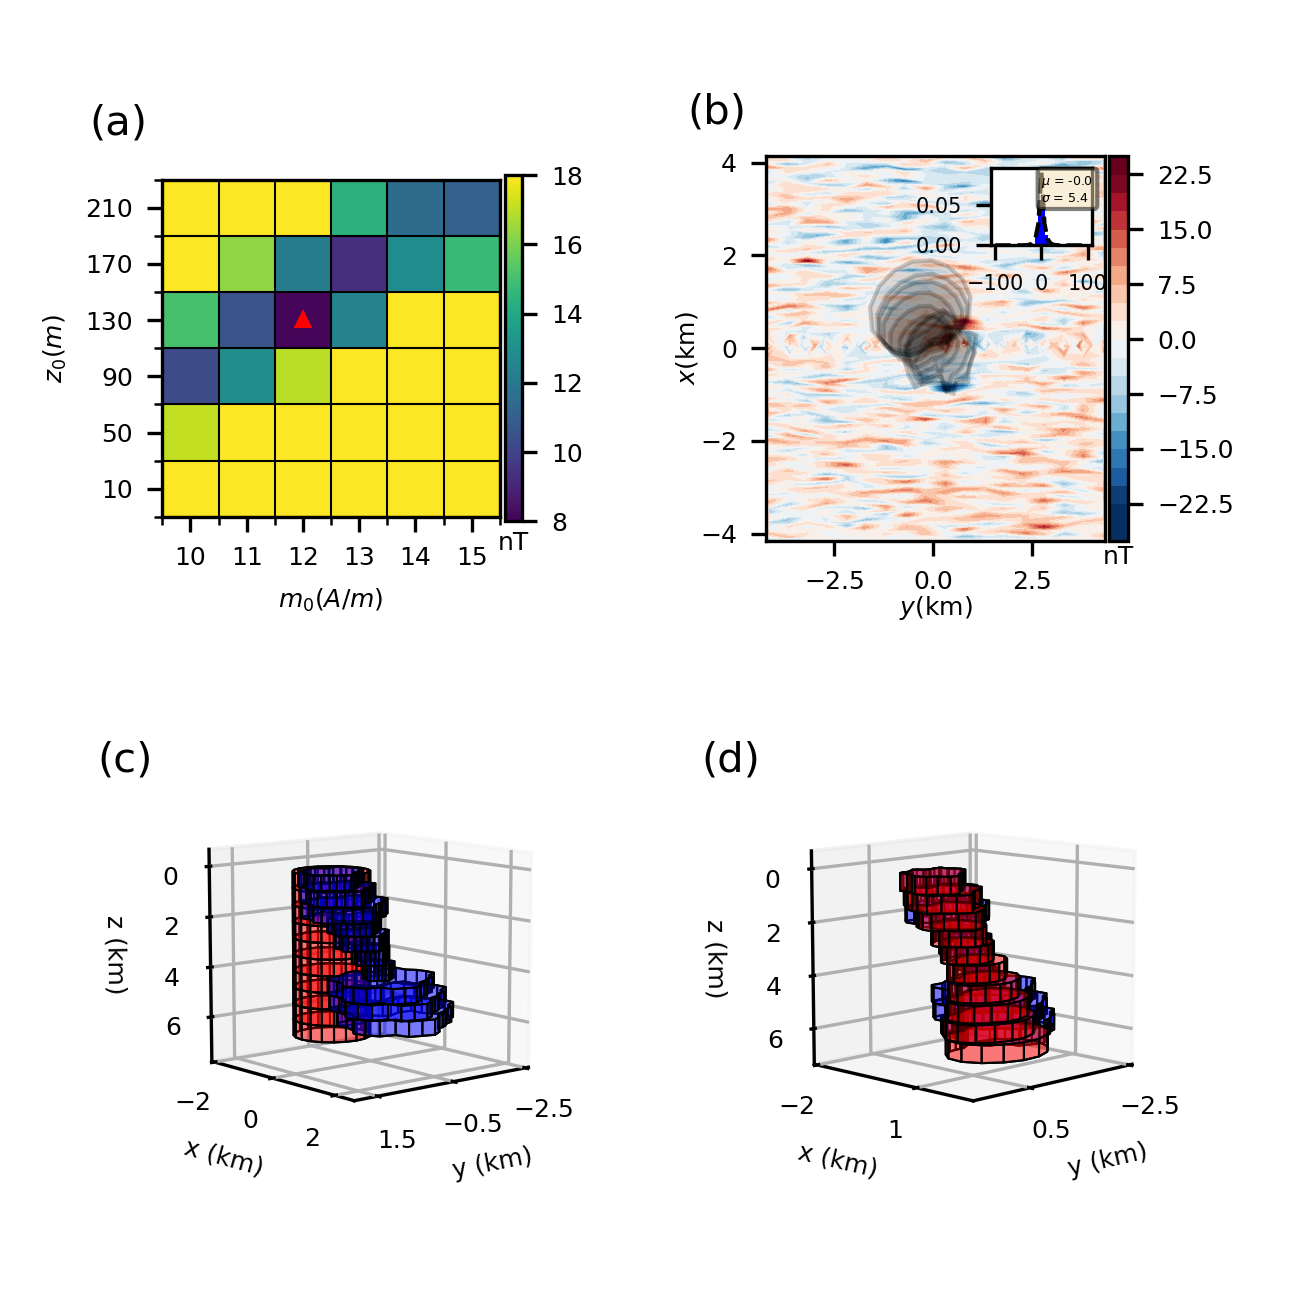
\includegraphics[width=\textwidth]{complex-l1-solution.png}
	\caption{Soluções L1 obtidas para o modelo da fonte alvo sem interferência. 
		(a) Mapa discreto da função objetivo produzida pelos modelos da malha de varredura para valores de profundidade do topo $z_{0}$ e intensidade de magnetização total $m_{0}$. 
		O triângulo vermelho representa os valores verdadeiros para $m_{0}$ e $z_{0}$, assim como os valores que definem a melhor solução L1.
		(b) Resíduos entre os dados contaminados com ruído (Figura \ref{fig:target_model}a) 
		e os dados preditos (não mostrados) produzidos pela melhor solução L1 (prismas vermelhos no painel d). 
		O histograma dos resíduos inserido em (b) mostra a curva Laplaciana ajustada (linha tracejada).
		Os polígonos cinzas representam as projeções horizontais de todos os prismas que compõe a melhor solução. 
		(c) e (d) Visualização em perspectiva da aproximação inicial (prismas vermelhos) e 
		a melhor solução (prismas vermelhos), respectivamente. Os prismas azuis são o modelo da fonte alvo. 
	}
	\label{fig:target_l1_result}
\end{figure}
\pagebreak


\section{Modelo complexo na presença de uma fonte não-alvo pequena}
\label{sec:target_source_with_small_interference}


O mapa da Figura \ref{fig:small_model}a representa a soma entre as anomalias de campo total produzidas pela fonte não-alvo pequena (Figura \ref{fig:small_model}b), cuja forma é exibida nas Figuras \ref{fig:small_model}c e \ref{fig:small_model}d, e aquela produzida pela fonte alvo simulada (Figura \ref{fig:target_model}a). 
A fonte não-alvo possui profundidade do topo em $0$ m, profundidade da base em $70$ m, 
centro em $(x, y) = (-250, 250)$, logo acima da parte mais rasa da fonte alvo, e o mesmo vetor magnetização total da fonte alvo.
Embora a nova anomalia RTP produzida com a fonte não-alvo (Figura 
\ref{fig:small_model_rtp}) tenha uma amplitude maior que a produzida pela fonte alvo isolada (Figura \ref{fig:target_model_rtp}), a extensão horizontal da área positiva não muda substancialmente e conduz a uma aproximação inicial
(Figuras \ref{fig:small_l2_result}c e \ref{fig:small_l1_result}c) igual àquela utilizada no teste anterior (Figuras \ref{fig:target_l2_result}c e 
\ref{fig:target_l1_result}c).

A Figura \ref{fig:small_l2_result} mostra as soluções L2 obtidas pela inversão da anomalia de campo total na Figura \ref{fig:small_model}a
com os seguintes pesos normalizados $\tilde{\alpha}_{\ell}$ (Equação \ref{eq:alphas}):
$\tilde{\alpha}_{1} = 10^{-5}$, $\tilde{\alpha}_{2} = 10^{-4}$, 
$\tilde{\alpha}_{3} = 10^{-4}$, $\tilde{\alpha}_{4} = 10^{-8}$, e 
$\tilde{\alpha}_{5} = 10^{-5}$.
A Figura \ref{fig:small_l2_result}a mostra que a melhor solução L2 possui profundidade do topo $z_{0}$ igual à verdadeira, porém possui uma intensidade de magnetização total $m_{0}$ superestimada. Por esse motivo, sua profundidade máxima 
($3046.8$ m) é muito distante da verdadeira ($6130$ m).
Essa solução produz valores de resíduos altos logo acima da fonte não-alvo 
(Figura \ref{fig:small_l2_result}b), mas esses resíduos diferem consideravelmente da anomalia de campo total produzida pela fonte não-alvo (Figura \ref{fig:small_model}b).
Isso significa que, nesse caso, a inversão não foi capaz de ignorar o efeito causado pela fonte não-alvo.
Além disso, a Figura \ref{fig:small_l2_result}d mostra que a melhor solução L2 não recupera a forma da fonte alvo.

A Figura \ref{fig:small_l1_result} mostra as soluções L1 obtidas pela inversão da anomalia de campo total exibida na Figura \ref{fig:small_model}a
com os mesmos pesos normalizados $\tilde{\alpha}_{\ell}$ (Equação \ref{eq:alphas})
utilizados para as soluções L2 (Figura \ref{fig:small_l2_result}).
Comparada à solução L2 mostrada na Figura \ref{fig:small_l2_result}, a melhor solução L1 apresenta uma intensidade de magnetização total menos superestimada (Figura 
\ref{fig:small_l1_result}a) e profundidade da base ($4993.7$ m) menos subestimada cerca de $ 1 $ km de diferença em relação à verdadeira ($6130$ m). Essa solução produz valores de resíduos (Figura \ref{fig:small_l1_result}b) 
próximos à anomalia de campo total produzida pela fonte não-alvo (Figura 
\ref{fig:small_model}b). 
Isso significa que, nesse caso, a performance do método foi mais eficaz em filtrar a anomalia de campo total não-alvo (Figura \ref{fig:small_model}b).
Como consequência, a solução L1 (Figura \ref{fig:small_l1_result}d) foi muito menos afetada pela fonte não-alvo e recuperou satisfatoriamente a forma da fonte alvo. 
A Tabela \ref{tab:small} mostra que para este teste a solução L1 é superior à solução L2 mesmo que a fonte não-alvo seja muito localizada e menor do que a fonte alvo.

\begin{table}[h]\label{tab:small}
	\caption{Valores dos vínculos na iteração final para as melhores soluções L2 e L1 da aplicação ao corpo complexo na presença de uma fonte não-alvo pequena (Eqs. \ref{eq:phi1}, \ref{eq:phi2}, \ref{eq:phi3}, \ref{eq:phi4} e \ref{eq:phi5}).}
	\centering
	\vspace{0.5cm}
	\begin{tabular}{c|ccccc}
		Vínculo & $ \varphi _1 $ & $ \varphi _2 $ &  $ \varphi _3 $ &  $ \varphi _4 $ &  $ \varphi _5 $ \\
		\hline
		Solução L2 & $ 0,45 $ & $ 20,75 $ & $ 1,94 $ & $ 0,29 $ & $ 1,94 $ \\ 
		Solução L1 & $ 0,25 $ & $ 3,56 $ & $ 0,83 $ & $ 0,22 $ & $ 4,49 $
	\end{tabular}
\end{table}

\pagebreak
\begin{figure}[!htb]
	\centering
	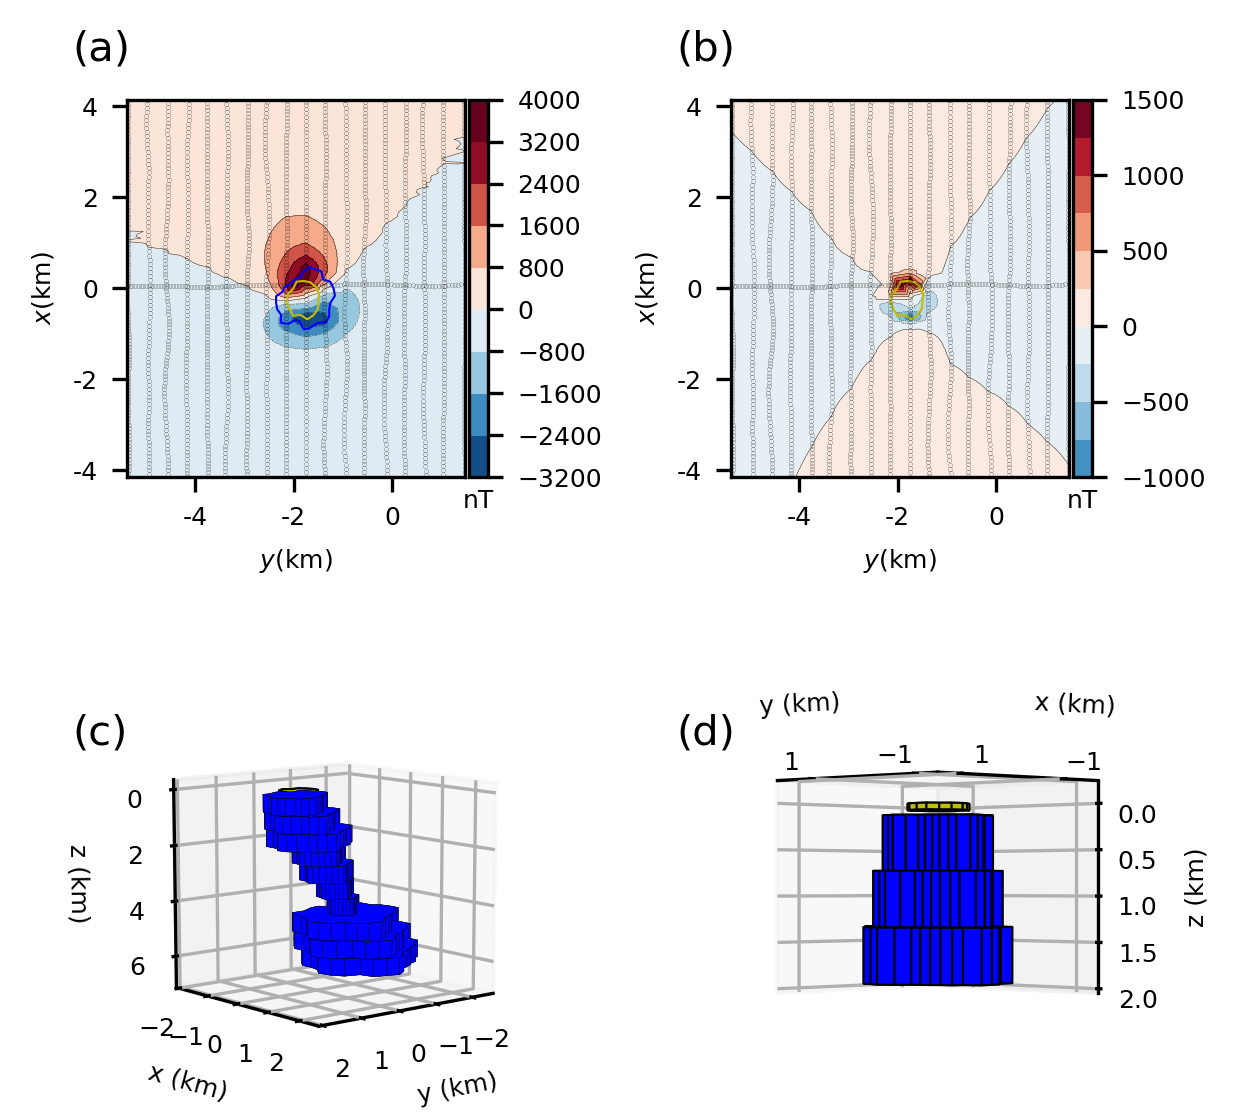
\includegraphics[width=\textwidth]{small_model_data.png}
	\caption{Modelo da fonte alvo com uma fonte não-alvo pequena.
		(a) Anomalia de campo total produzida pelas fontes alvo e não-alvo
		(prismas azuis e amarelos nos painéis c e d). Os pontos pretos representam os pontos de observação. Os polígonos azul e amarelo são as projeções horizontais das fontes alvo e não-alvo, respectivamente.
		(b) A anomalia de campo total produzida pela fonte não-alvo. 
		(c) Visualização em perspectiva da fonte alvo (prismas azuis) e da fonte não-alvo (prisma amarelo). 
		(d) Visualização em perspectiva aproximada das fontes alvo (prismas azuis) e não-alvo (prisma amarelo).
	}
	\label{fig:small_model}
\end{figure}
\pagebreak
\begin{figure}[!htb]
	\centering
	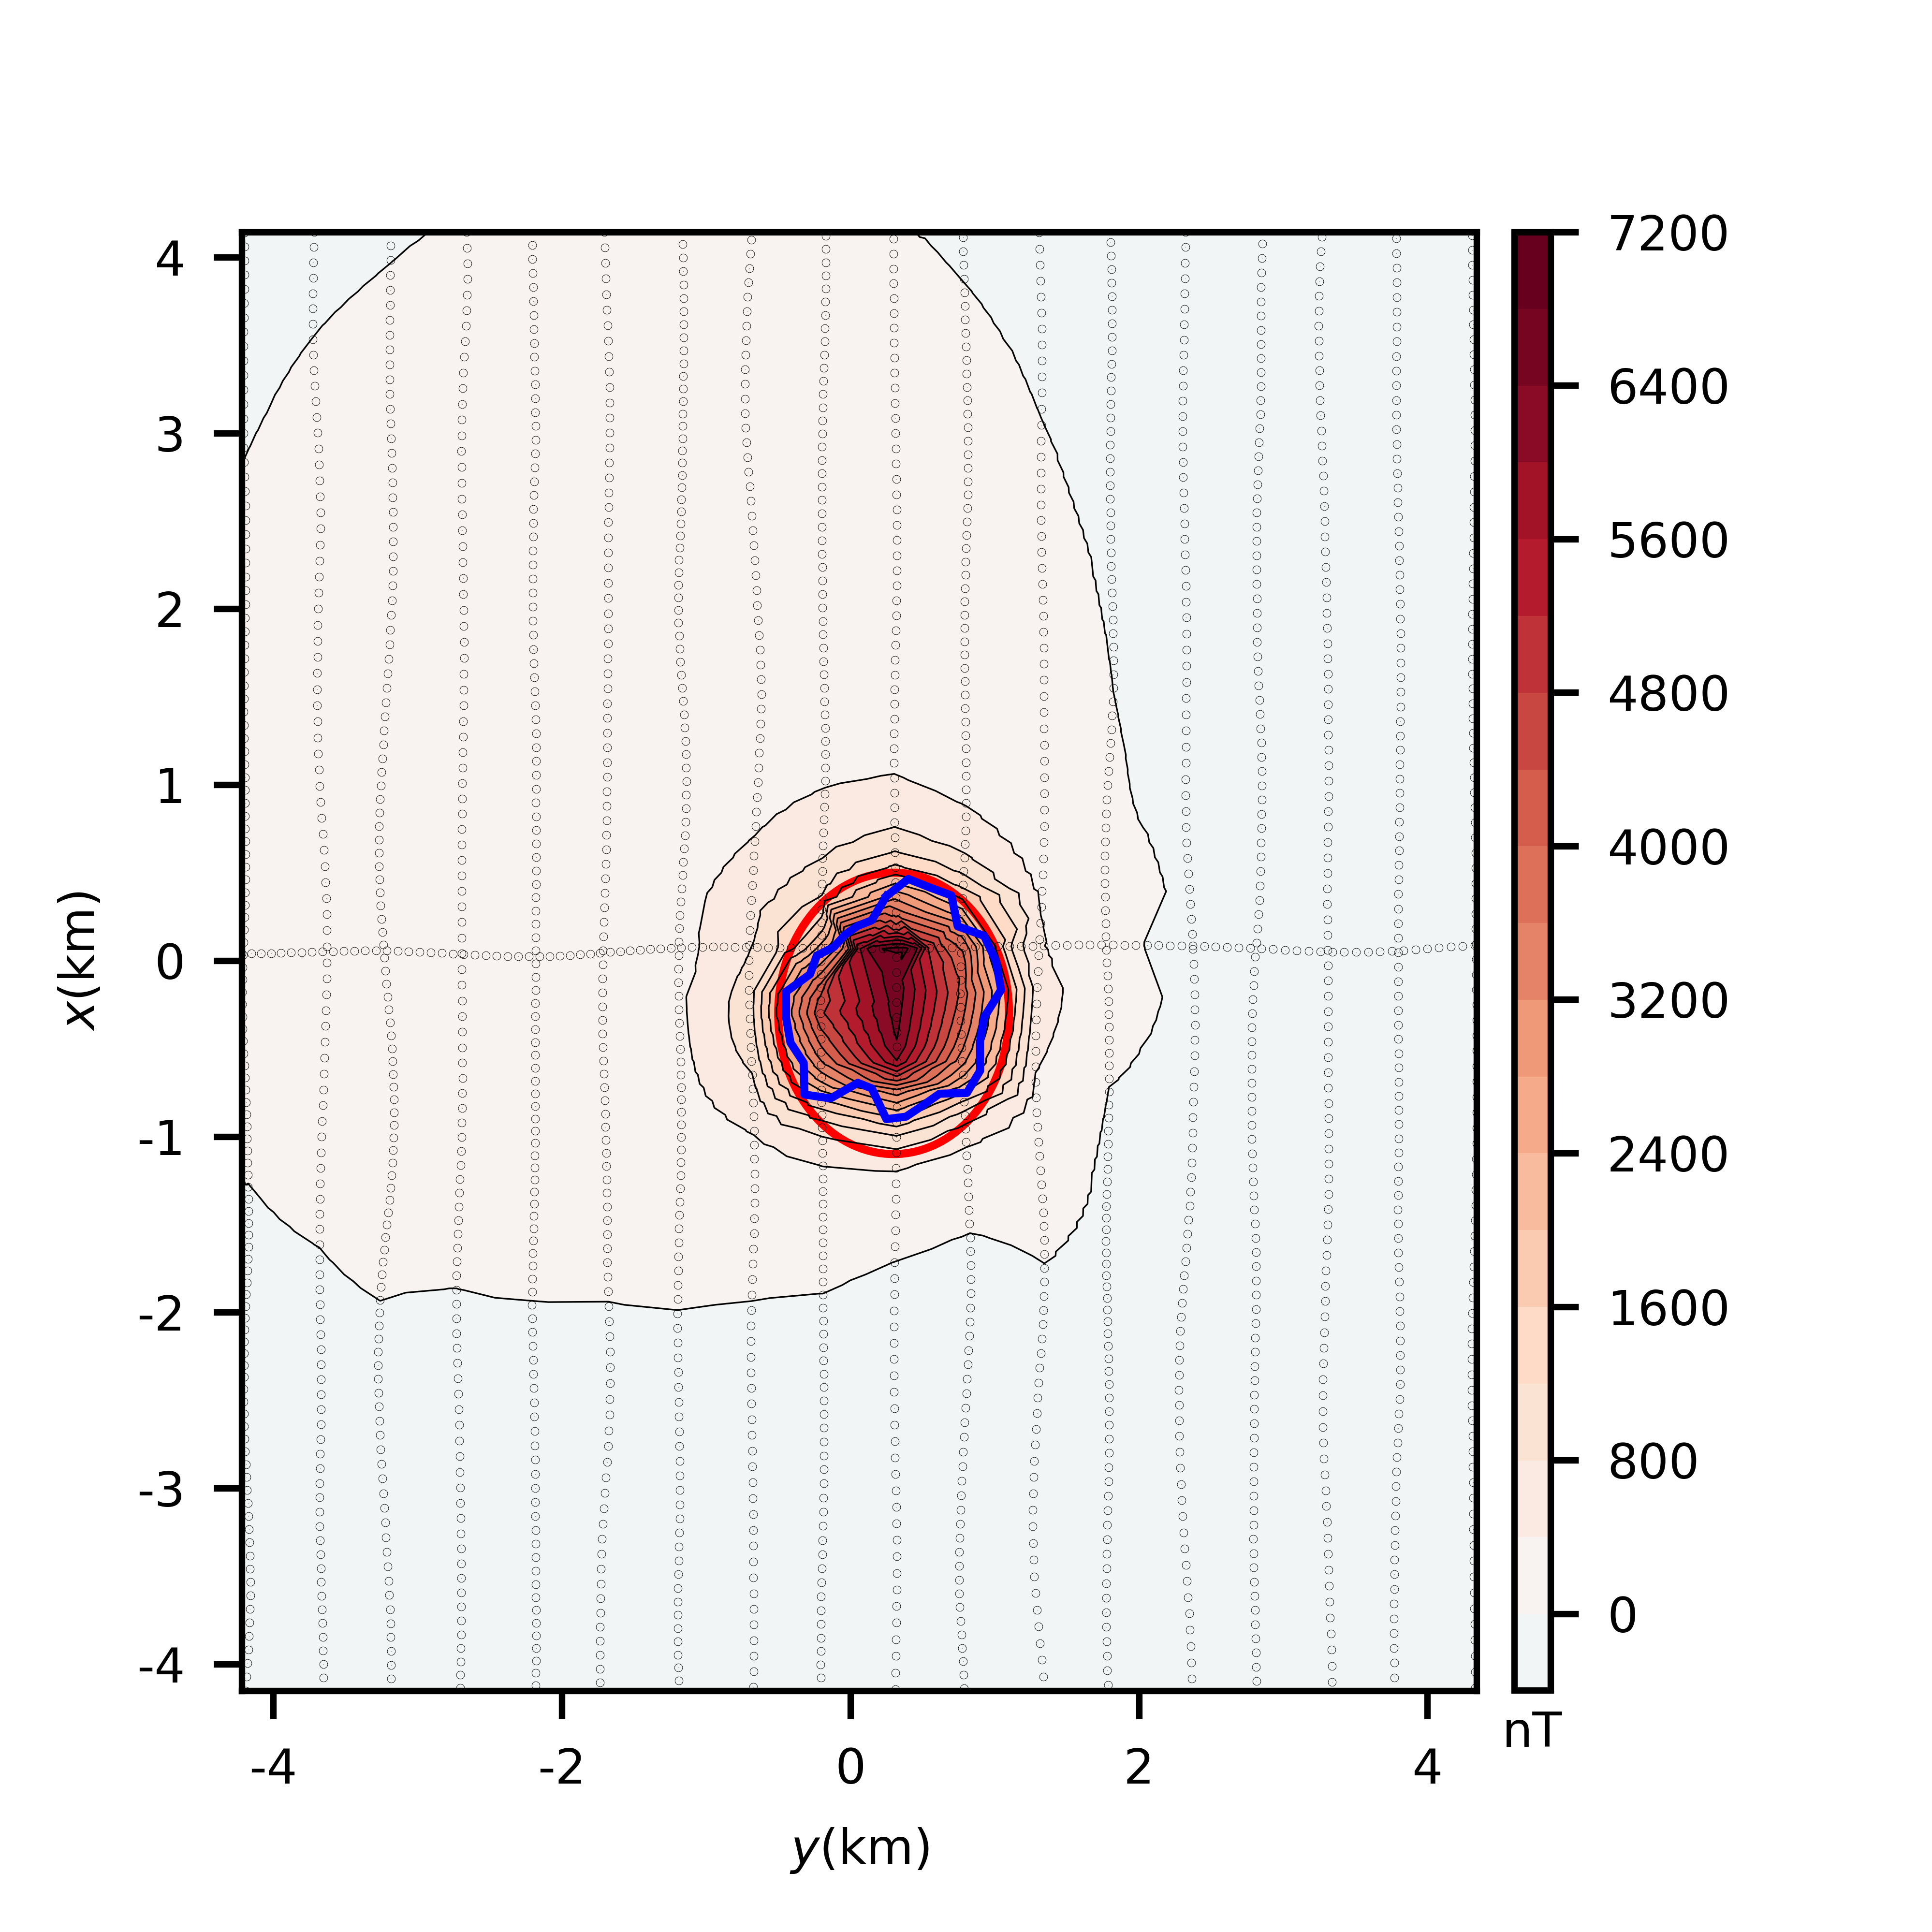
\includegraphics[width=\textwidth]{small_rtp.png}
	\caption{Anomalia RTP estimada produzida pela fonte alvo com uma fonte não-alvo pequena. 
		A anomalia RTP mostra valores predominantemente positivos logo acima da fonte alvo. Os pontos pretos representam os pontos de observação. As linhas azuis e vermelhas correspondem, respectivamente, às projeções horizontais da porção mais rasa da fonte alvo e da aproximação inicial utilizada nas inversões subsequentes (prismas vermelhos nas Figuras \ref{fig:small_l2_result}c e 
		\ref{fig:small_l1_result}c).
	}
	\label{fig:small_model_rtp}
\end{figure}
\pagebreak
\begin{figure}[!htb]
	\centering
	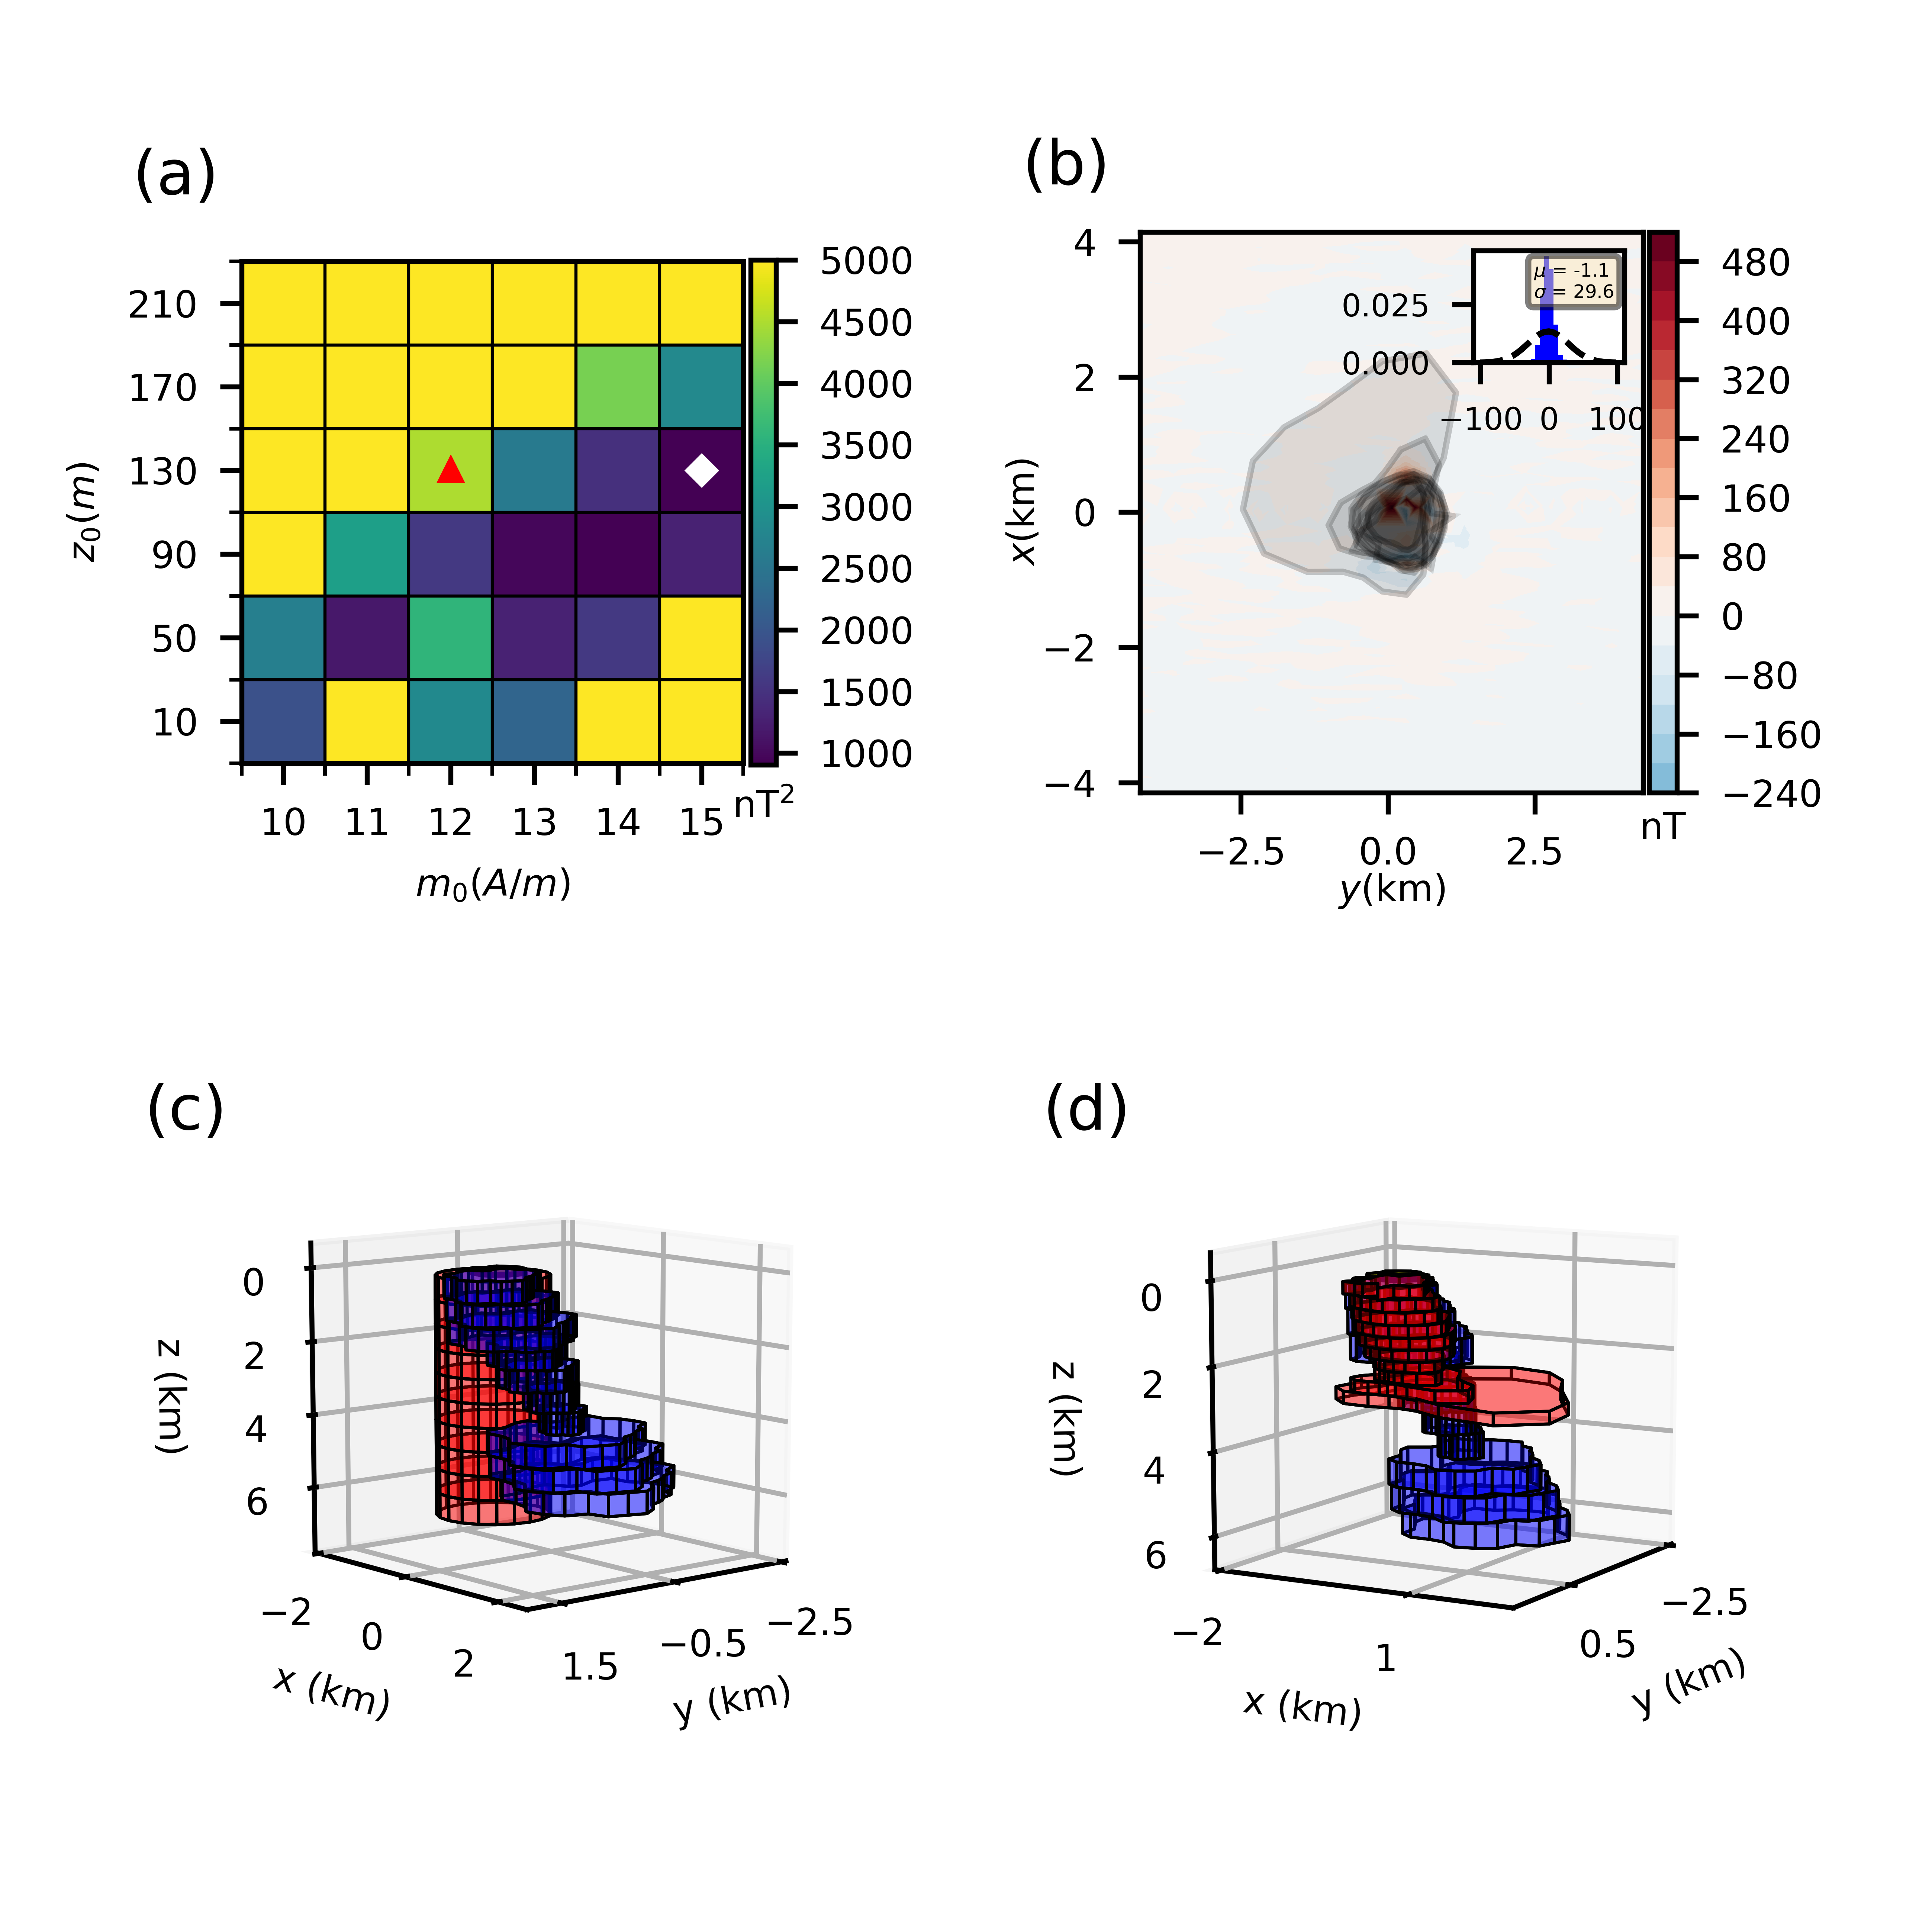
\includegraphics[width=\textwidth]{small-l2-solution.png}
	\caption{Soluções L2 obtidas para o modelo da fonte alvo com uma fonte não-alvo pequena. 
		(a) Mapa discreto da função objetivo produzida pelos modelos da malha de varredura para valores de profundidade do topo $z_{0}$ e intensidade de magnetização total $m_{0}$. 
		Os valores verdadeiros de $m_{0}$ e $z_{0})$ e aqueles que definem a melhor solução L2 são representados pelo triângulo vermelho e pelo losango branco, respectivamente.
		(b) Resíduos entre os dados contaminados com ruído (Figura \ref{fig:small_model}a) 
		e os dados preditos (não mostrados) produzidos pela melhor solução L2 (prismas vermelhos no painel d). 
		O histograma dos resíduos inserido em (b) mostra a curva Gaussiana ajustada (linha tracejada).
		Os polígonos cinzas representam as projeções horizontais de todos os prismas que compõe a melhor solução. 
		(c) e (d) Visualização em perspectiva da aproximação inicial (prismas vermelhos) e 
		a melhor solução (prismas vermelhos), respectivamente. Os prismas azuis são o modelo da fonte alvo.
	}
	\label{fig:small_l2_result}
\end{figure}
\pagebreak
\begin{figure}[!htb]
	\centering
	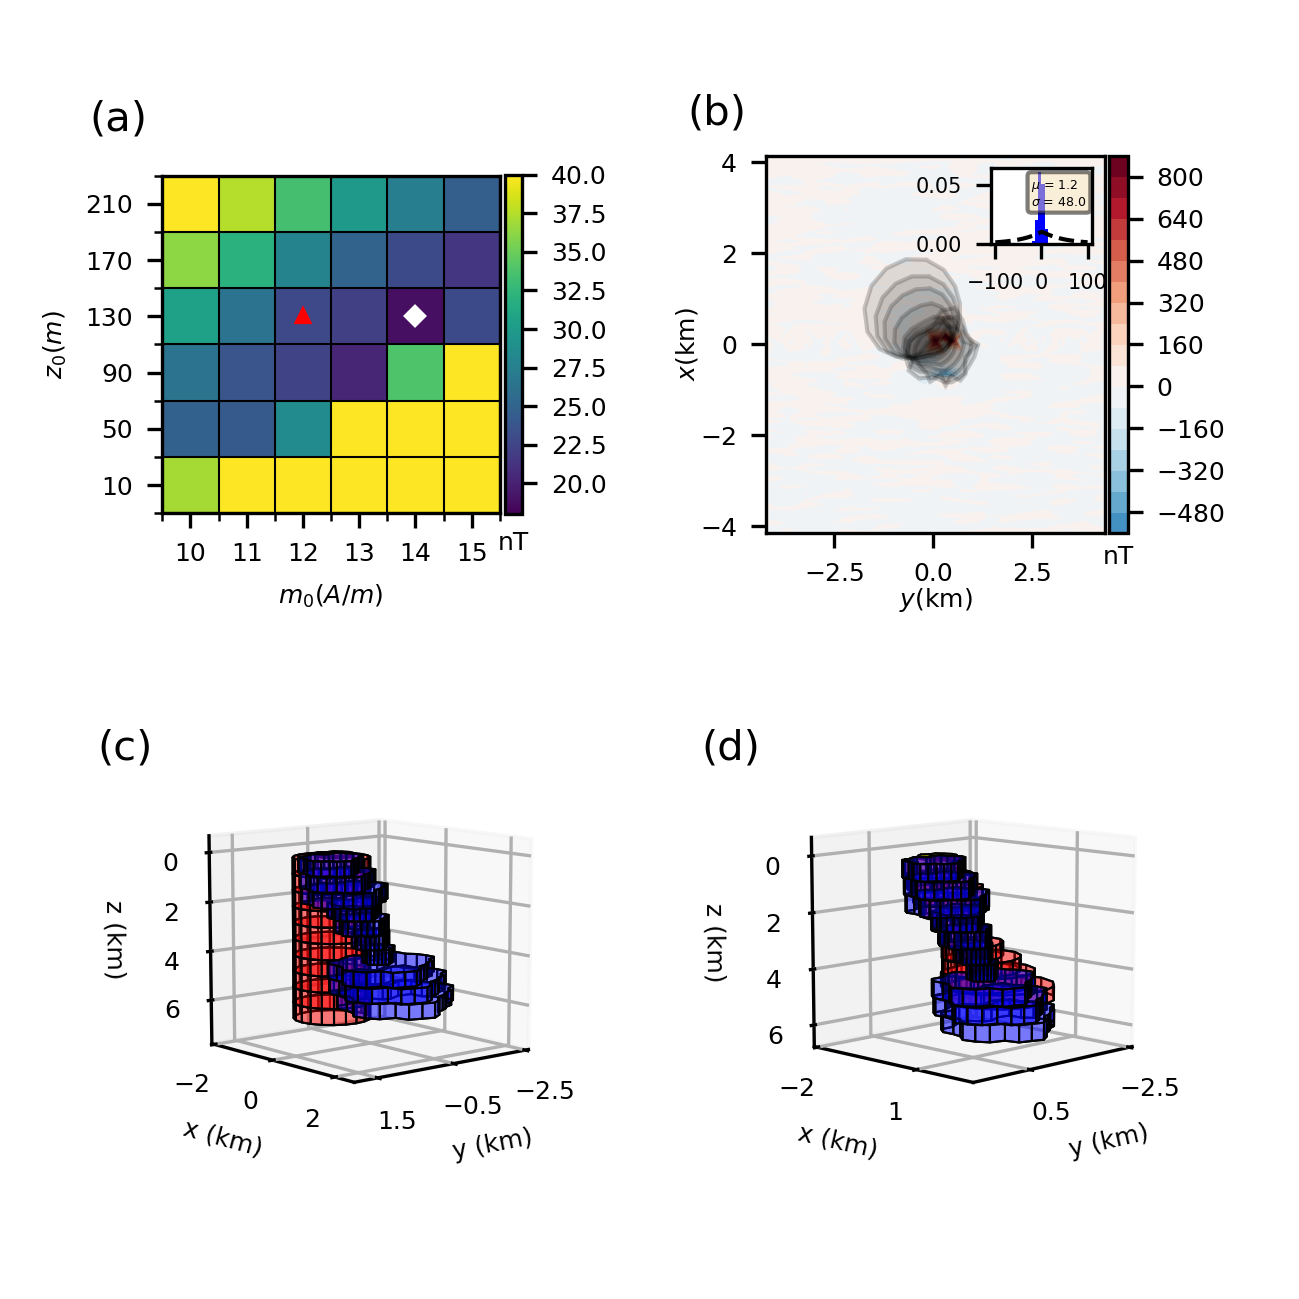
\includegraphics[width=\textwidth]{small-l1-solution.png}
	\caption{Soluções L1 obtidas para o modelo da fonte alvo com uma fonte não-alvo pequena. 
		(a) Mapa discreto da função objetivo produzida pelos modelos da malha de varredura para valores de profundidade do topo $z_{0}$ e intensidade de magnetização total $m_{0}$. 
		Os valores verdadeiros de $m_{0}$ e $z_{0})$ e aqueles que definem a melhor solução L1 são representados pelo triângulo vermelho e pelo losango branco, respectivamente.
		(b) Resíduos entre os dados contaminados com ruído (Figura \ref{fig:fig:small_model}a) 
		e os dados preditos (não mostrados) produzidos pela melhor solução L1 (prismas vermelhos no painel d). 
		O histograma dos resíduos inserido em (b) mostra a curva Gaussiana ajustada (linha tracejada).
		Os polígonos cinzas representam as projeções horizontais de todos os prismas que compõe a melhor solução. 
		(c) e (d) Visualização em perspectiva da aproximação inicial (prismas vermelhos) e 
		a melhor solução (prismas vermelhos), respectivamente. Os prismas azuis são o modelo da fonte alvo. 
	}
	\label{fig:small_l1_result}
\end{figure}
\pagebreak
\section{Modelo complexo na presença de uma fonte não-alvo grande}
\label{sec:target_source_with_large_interference}

O mapa da Figura \ref{fig:thick_model}a representa a soma entre as anomalias de campo total produzidas pela fonte não-alvo pequena (Figura \ref{fig:thick_model}b), cuja forma é exibida nas Figuras \ref{fig:thick_model}c e \ref{fig:thick_model}d, e aquela produzida pela fonte alvo simulada (Figura \ref{fig:target_model}a).
A fonte não-alvo possui profundidade do topo em $0$ m, profundidade da base em $500$ m, 
centro em $(x, y) = (500, 1500)$, ao lado do topo da fonte alvo, e o mesmo vetor magnetização total da fonte alvo.
Neste caso, a fonte não-alvo estende consideravelmente a área positiva da anomalia RTP (Figura \ref{fig:thick_model_rtp}) em comparação com a da fonte alvo isolada (Figura \ref{fig:target_model_rtp}). Entretanto, ainda é possível identificar os limites laterais da fonte alvo e gerar a mesma aproximação inicial usada nos testes anteriores.


A Figura \ref{fig:thick_l2_result} mostra as soluções L2 obtidas pela inversão da anomalia de campo total na Figura \ref{fig:thick_model}a
com os seguintes pesos normalizados $\tilde{\alpha}_{\ell}$ (Equação \ref{eq:alphas}):
$\tilde{\alpha}_{1} = 10^{-3}$, $\tilde{\alpha}_{2} = 10^{-5}$, 
$\tilde{\alpha}_{3} = 10^{-4}$, $\tilde{\alpha}_{4} = 10^{-6}$, e 
$\tilde{\alpha}_{5} = 10^{-6}$.
Como podemos ver, a melhor solução L2 não recupera os valores da profundidade do topo $z_{0}$ e nem da intensidade de magnetização total $m_{0}$, assim como não recuperou a forma da fonte alvo.
A estimativa da profundidade da base ($1931,0$ m) é muito distante da verdadeira ($6130$ m).
Comparado ao valor verdadeiro, a profundidade do topo estimada $z_{0}$ está deslocada em direção à da fonte não-alvo.
Nesse caso, a fonte não-alvo induz severamente ao erro da estimativa da geometria do corpo (Figura \ref{fig:thick_l2_result}d).

A Figura \ref{fig:thick_l1_result} mostra as soluções L1 obtidas pela inversão da anomalia de campo total mostrada na Figura \ref{fig:thick_model}a
com os seguintes pesos normalizados $\tilde{\alpha}_{\ell}$ (Equação \ref{eq:alphas})utilizados para as soluções L2 (Figura \ref{fig:thick_l2_result}).
A melhor solução L1 (Figura \ref{fig:thick_l1_result}) filtra parcialmente a anomalia de campo total não-alvo (Figura \ref{fig:thick_model}b) e recupera as principais feições da fonte alvo sintética, assim como a profundidade do topo $z_{0}$ e a intensidade de magnetização total $m_{0}$ verdadeiras.
Essa solução estima a profundidade da base ($5820.4$ m) melhor do que a do teste anterior, no entanto, a solução é inferior à mostrada no teste anterior em filtrar a anomalia de campo total não-alvo e também em recuperar a geometria da fonte alvo.
Apesar disso, a Tabela \ref{tab:thick} mostra que ela é significativamente superior à melhor solução L2 (Figura \ref{fig:thick_l2_result}) obtida pela inversão do mesmo dado, uma vez que é muito menos afetada pela presença de uma grande fonte não-alvo.

\begin{table}[h]\label{tab:thick}
	\caption{Valores dos vínculos na iteração final para as melhores soluções L2 e L1 da aplicação ao corpo complexo na presença de uma fonte não-alvo grande (Eqs. \ref{eq:phi1}, \ref{eq:phi2}, \ref{eq:phi3}, \ref{eq:phi4} e \ref{eq:phi5}).}
	\centering
	\vspace{0.5cm}
	\begin{tabular}{c|ccccc}
		Vínculo & $ \varphi _1 $ & $ \varphi _2 $ &  $ \varphi _3 $ &  $ \varphi _4 $ &  $ \varphi _5 $ \\
		\hline
		Solução L2 & $ 145,68 $ & $ 2,13 $ & $ 7,15 $ & $ 2,36 $ & $3,88 \times 10^{-2} $ \\ 
		Solução L1 & $ 16,17 $ & $ 0,42 $ & $ 2,36 $ & $ 1,58 $ & $ 0,38 $
	\end{tabular}
\end{table}

\pagebreak
\begin{figure}[!htb]
	\centering
	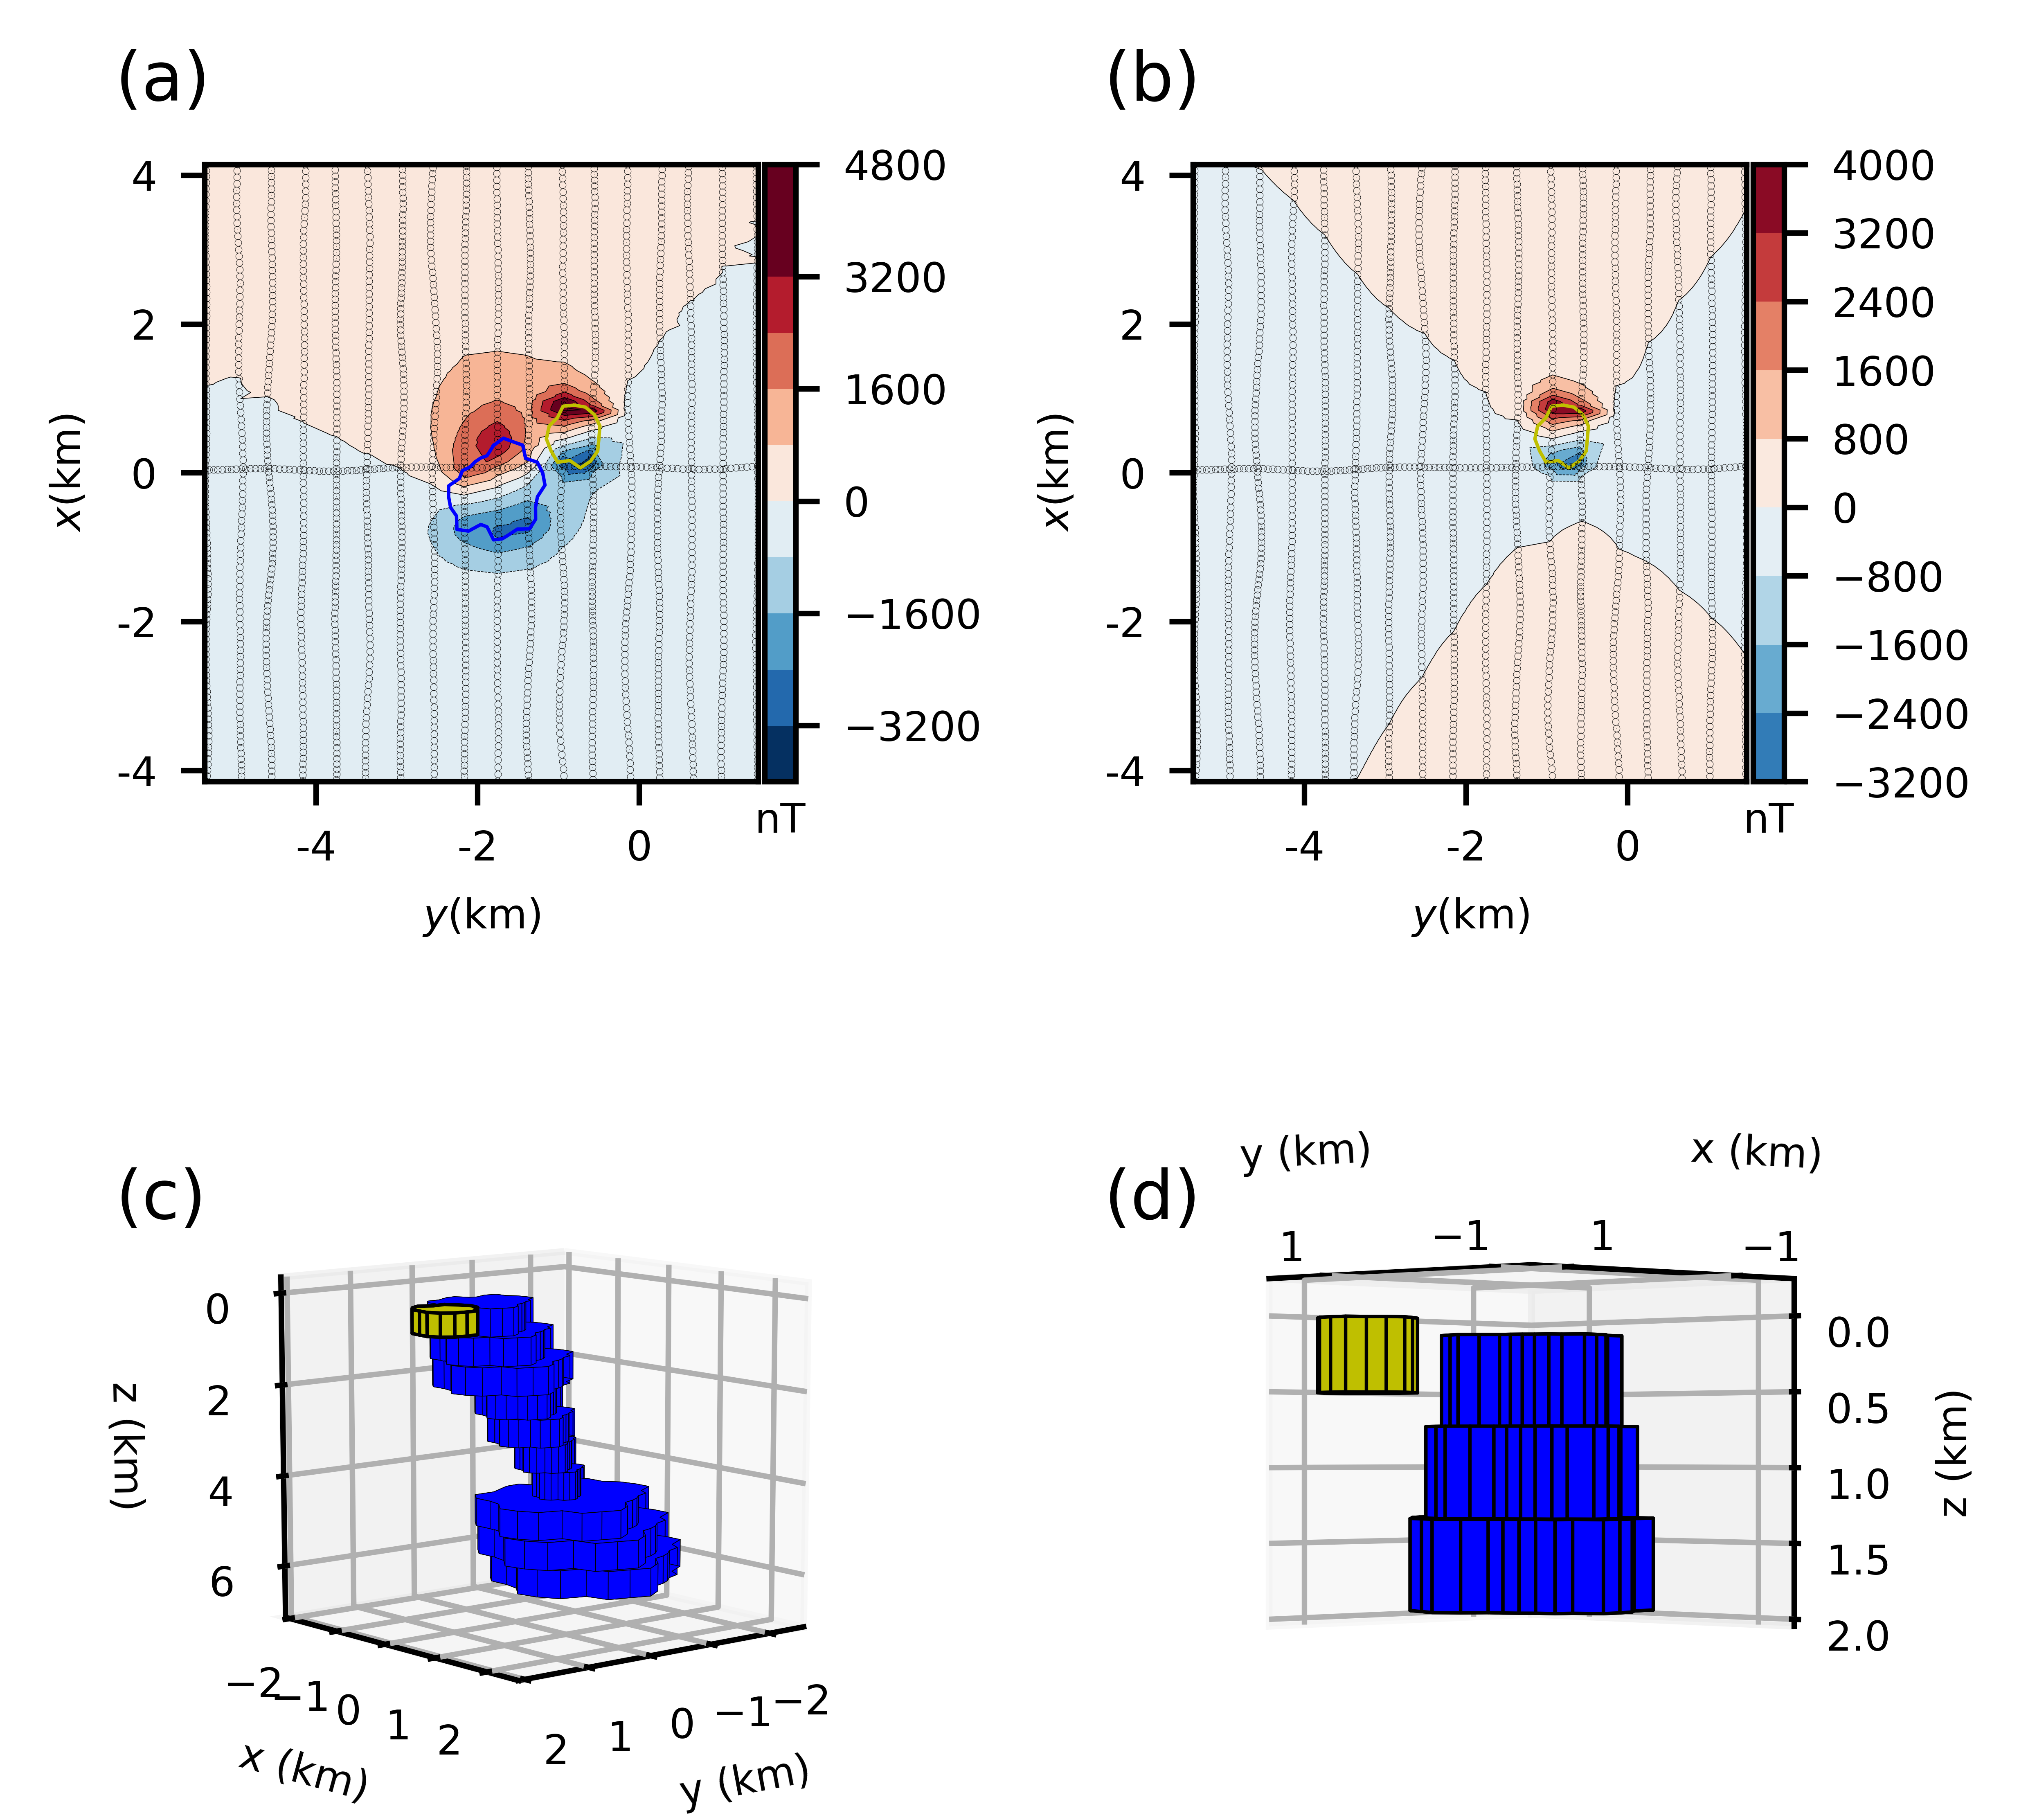
\includegraphics[width=\textwidth]{thick_model_data.png}
	\caption{Modelo da fonte alvo com uma fonte não-alvo grande.
		(a) Anomalia de campo total produzida pelas fontes alvo e não-alvo
		(prismas azuis e amarelos nos painéis c e d). Os pontos pretos representam os pontos de observação. Os polígonos azul e amarelo são as projeções horizontais das fontes alvo e não-alvo, respectivamente.
		(b) A anomalia de campo total produzida pela fonte não-alvo. 
		(c) Visualização em perspectiva da fonte alvo (prismas azuis) e da fonte não-alvo (prisma amarelo). 
		(d) Visualização em perspectiva aproximada das fontes alvo (prismas azuis) e não-alvo (prisma amarelo).
	}
	\label{fig:thick_model}
\end{figure}
\pagebreak

\begin{figure}[!htb]
	\centering
	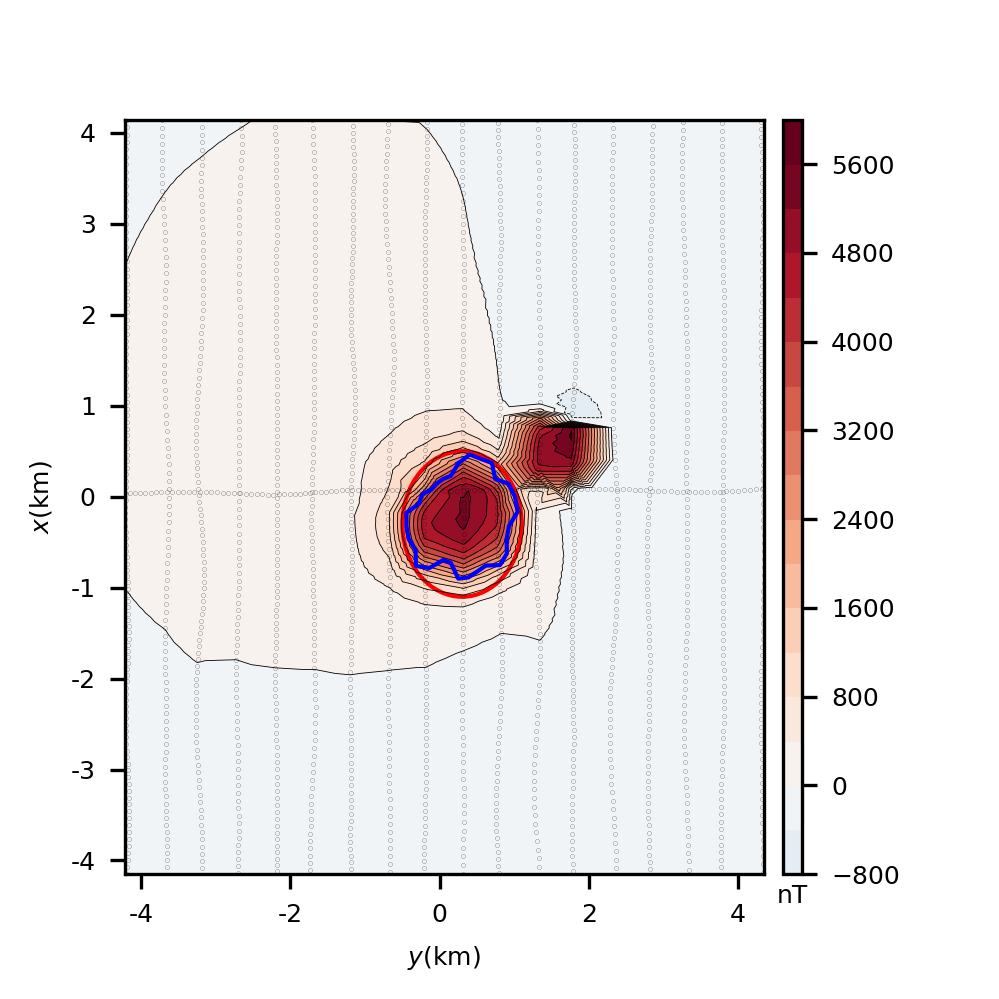
\includegraphics[width=\textwidth]{thick_rtp.png}
	\caption{Anomalia RTP estimada produzida pela fonte alvo com uma fonte não-alvo grande. 
		A anomalia RTP mostra valores predominantemente positivos logo acima das fontes alvo e não-alvo. Os pontos pretos representam os pontos de observação. As linhas azuis e vermelhas correspondem, respectivamente, às projeções horizontais da porção mais rasa da fonte alvo e da aproximação inicial utilizada nas inversões subsequentes (prismas vermelhos nas Figuras \ref{fig:thick_l2_result}c e 
		\ref{fig:thick_l1_result}c).
	}
	\label{fig:thick_model_rtp}
\end{figure}
\pagebreak
\begin{figure}[!htb]
	\centering
	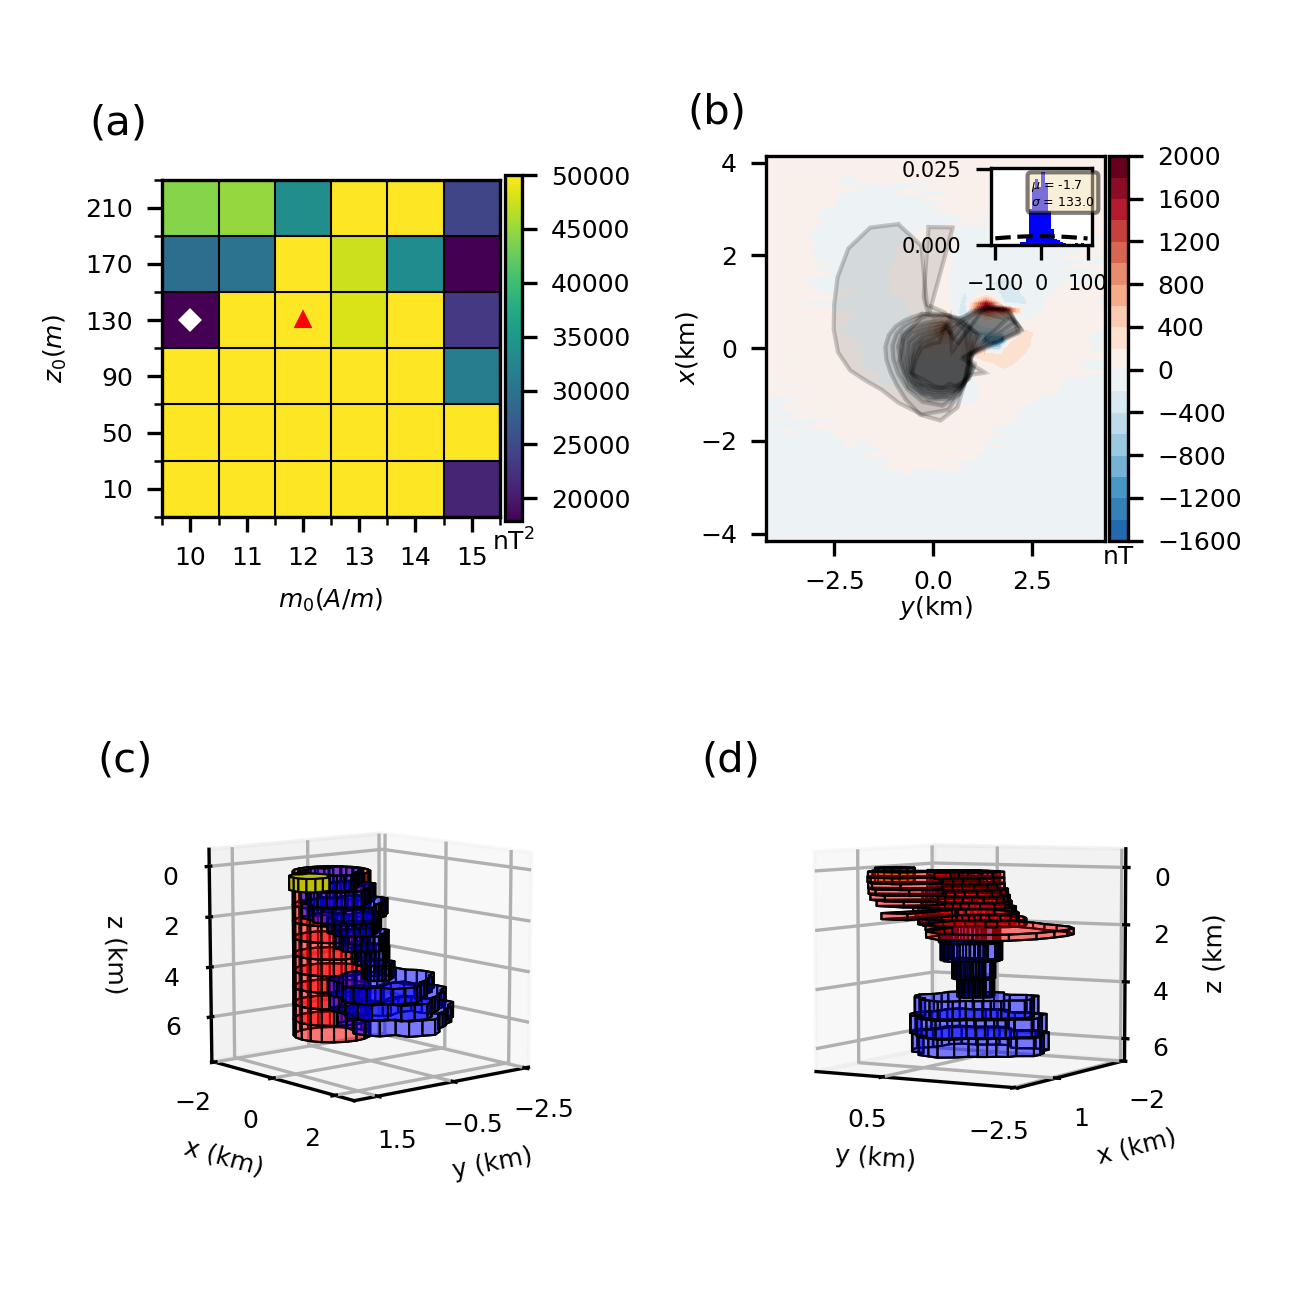
\includegraphics[width=\textwidth]{thick-l2-solution.png}
	\caption{Soluções L2 obtidas para o modelo da fonte alvo com uma fonte não-alvo grande. 
	(a) Mapa discreto da função objetivo produzida pelos modelos da malha de varredura para valores de profundidade do topo $z_{0}$ e intensidade de magnetização total $m_{0}$. 
	Os valores verdadeiros de $m_{0}$ e $z_{0})$ e aqueles que definem a melhor solução L2 são representados pelo triângulo vermelho e pelo losango branco, respectivamente.
	(b) Resíduos entre os dados contaminados com ruído (Figura \ref{fig:thick_model}a) 
	e os dados preditos (não mostrados) produzidos pela melhor solução L2 (prismas vermelhos no painel d). 
	O histograma dos resíduos inserido em (b) mostra a curva Gaussiana ajustada (linha tracejada).
	Os polígonos cinzas representam as projeções horizontais de todos os prismas que compõe a melhor solução. 
	(c) e (d) Visualização em perspectiva da aproximação inicial (prismas vermelhos) e 
	a melhor solução (prismas vermelhos), respectivamente. Os prismas azuis são o modelo da fonte alvo. 
	}
	\label{fig:thick_l2_result}
\end{figure}
\pagebreak
\begin{figure}[!htb]
	\centering
	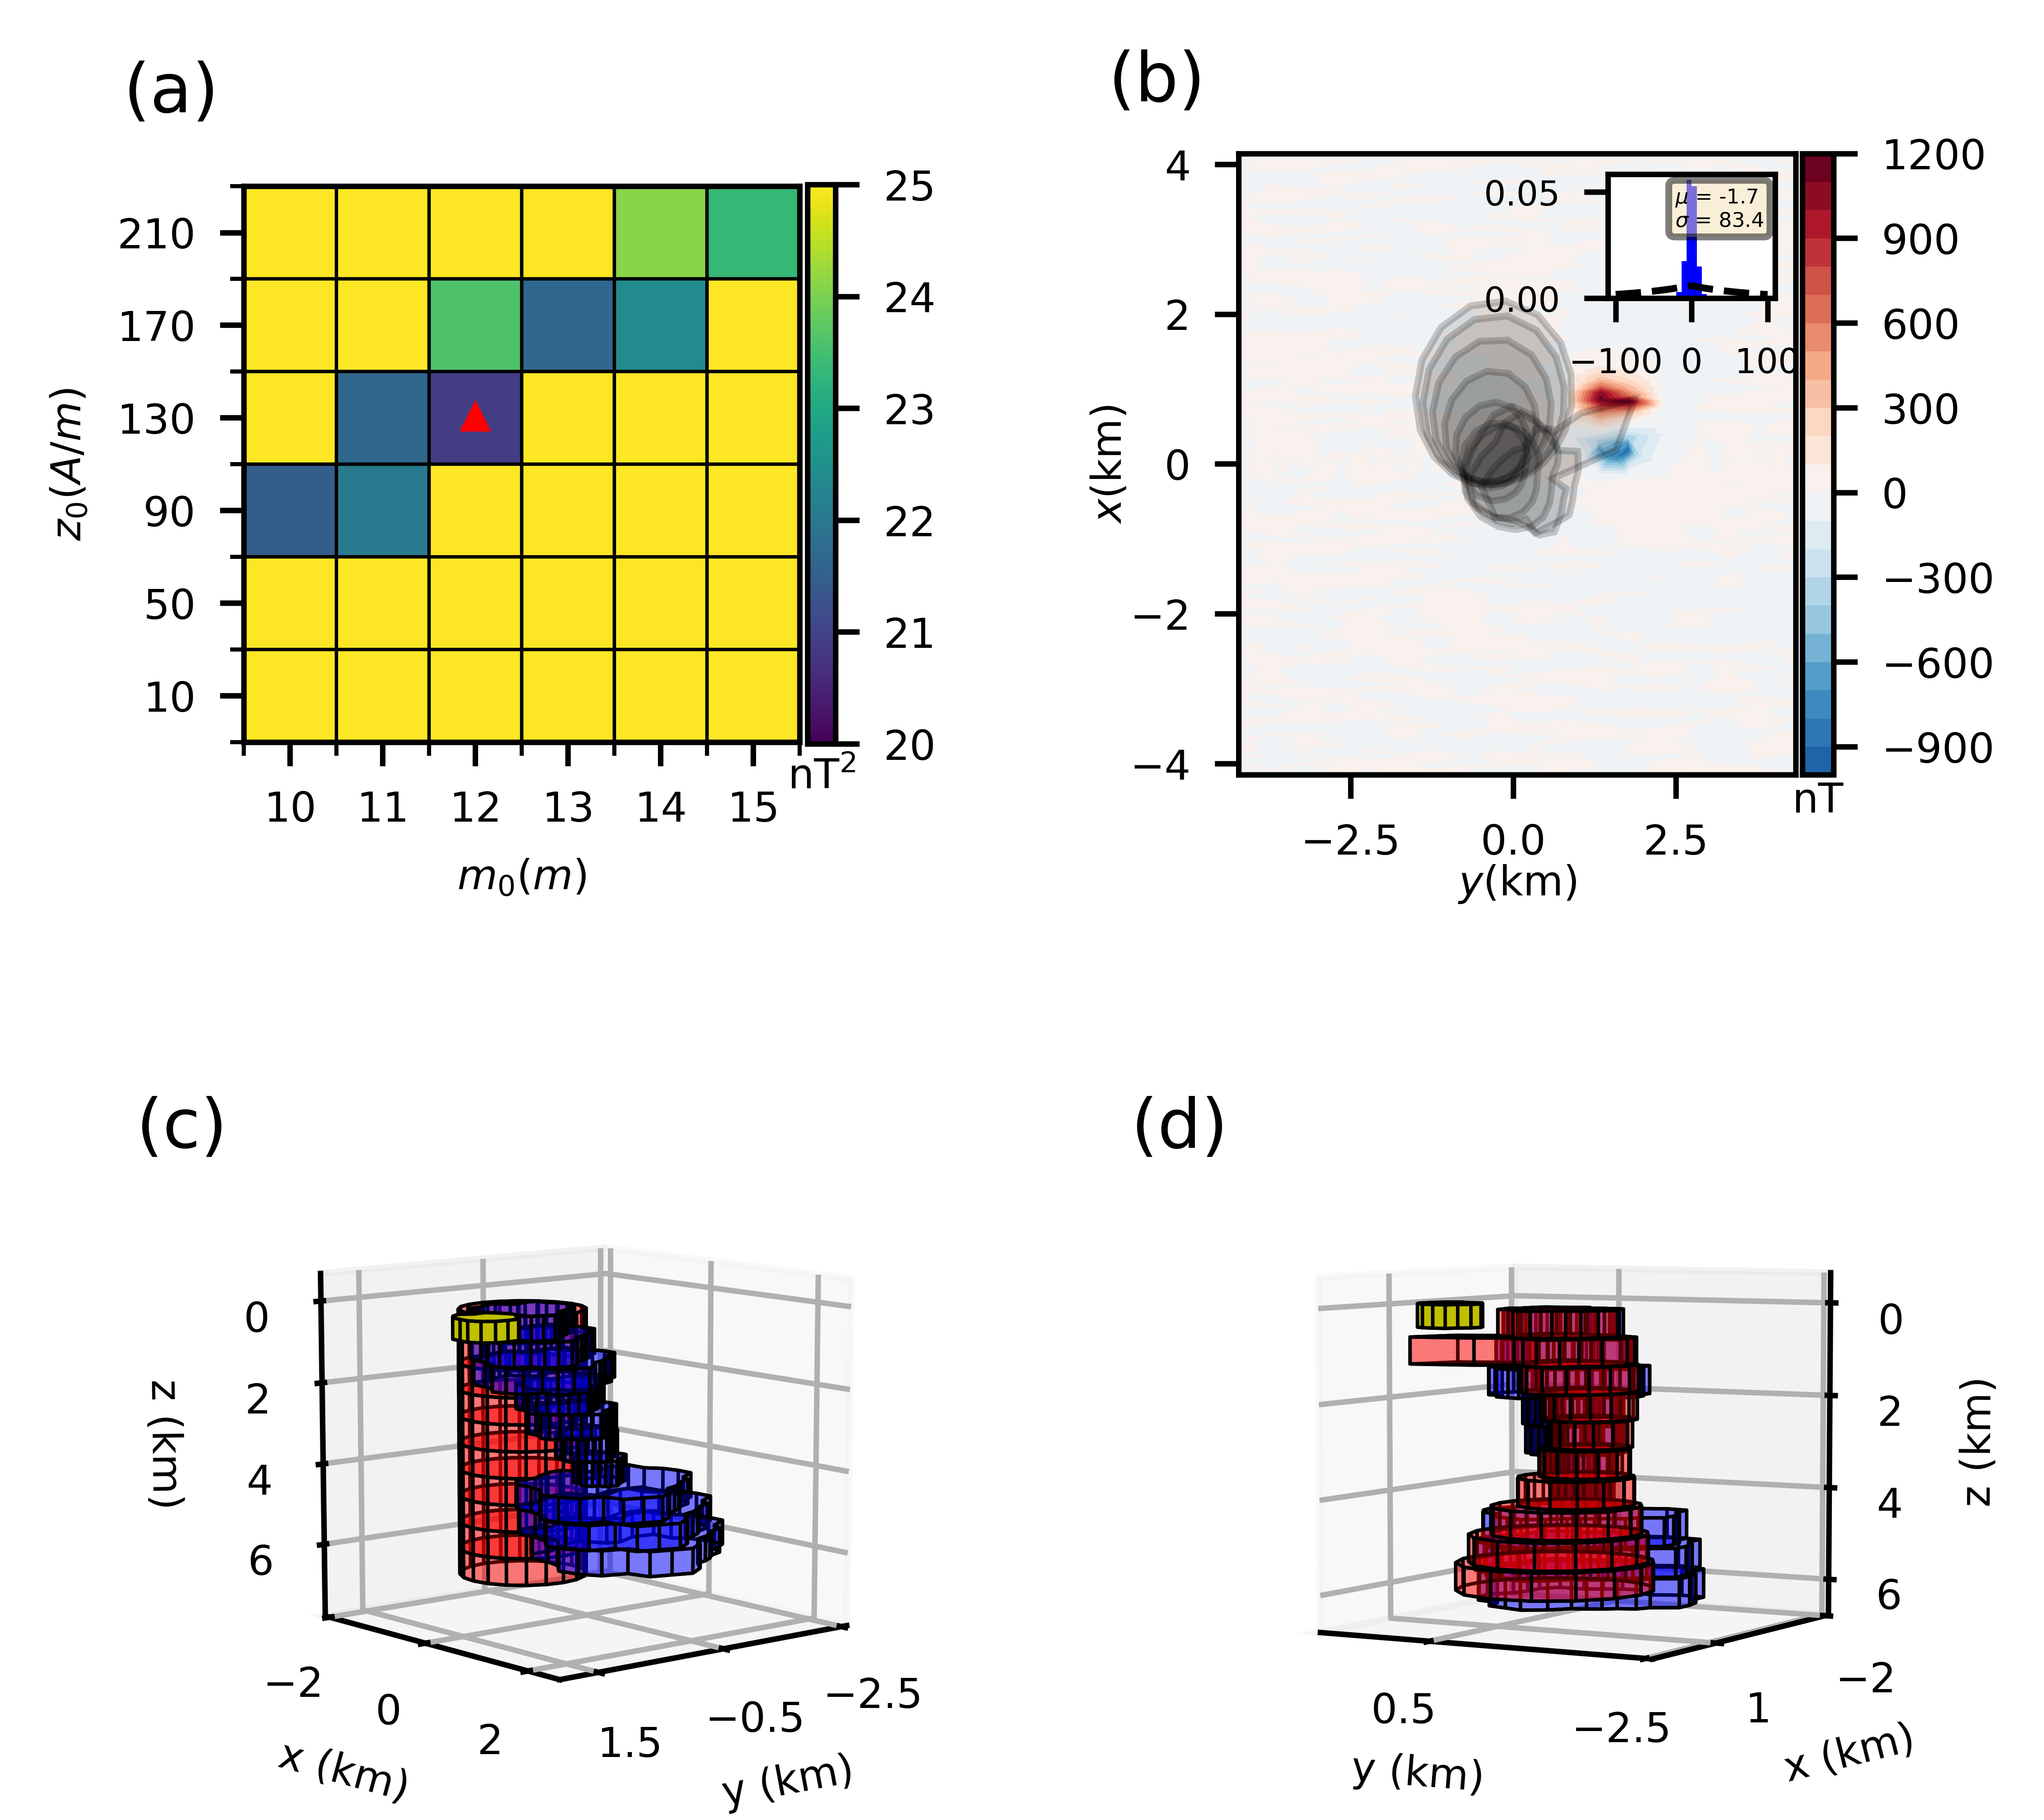
\includegraphics[width=\textwidth]{thick-l1-solution.png}
	\caption{Soluções L1 obtidas para o modelo da fonte alvo com uma fonte não-alvo grande. 
		(a) Mapa discreto da função objetivo produzida pelos modelos da malha de varredura para valores de profundidade do topo $z_{0}$ e intensidade de magnetização total $m_{0}$. 
		Ambos valores verdadeiros de $m_{0}$ e $z_{0})$ e aqueles que definem a melhor solução L1 são representados pelo triângulo vermelho.
		(b) Resíduos entre os dados contaminados com ruído (Figura \ref{fig:thick_model}a) 
		e os dados preditos (não mostrados) produzidos pela melhor solução L1 (prismas vermelhos no painel d). 
		O histograma dos resíduos inserido em (b) mostra a curva Gaussiana ajustada (linha tracejada).
		Os polígonos cinzas representam as projeções horizontais de todos os prismas que compõe a melhor solução. 
		(c) e (d) Visualização em perspectiva da aproximação inicial (prismas vermelhos) e 
		a melhor solução (prismas vermelhos), respectivamente. Os prismas azuis são o modelo da fonte alvo. 
	}
	\label{fig:thick_l1_result}
\end{figure}
\pagebreak
  \chapter{Aplicação a dados reais}


\section{Complexo de Anitápolis}
\label{subsec:anitapolis_complex}


O complexo alcalino-carbonatítico de Anitápolis forma um corpo circular 
($\approx 6$ km$^{2}$) que contém magnetita e leucogranitos do Cretáceo Inferior ($132$ Ma), aparentemente na mesma época do derramamento basáltico da formação Serra Geral ($133-130$ Ma) na Bacia do Paraná \citep{scheibe_etal2005, gomes_etal2018}. 
De acordo com \citet{riccomini_etal2005} e \citet{gomes_etal2018}, 
este complexo de Anitápolis não mostra um controle estrutural claro e ainda há debate sobre sua intrusão. 
Por exemplo, \citet{melcher_coutinho1966} propôs a influência de falhas orientadas preferencialmente em N-S
enquanto que \citet{horbach_marimon1980} e \citet{scheibe_etal2005} consideram que o complexo é controlado por lineamentos N30O e L-O, respectivamente.

As Figuras \ref{fig:anitapolis_data}a e \ref{fig:anitapolis_data}b exibem a anomalia de campo total observada e o campo regional estimado sobre o complexo de Anitápolis, respectivamente.
O levantamento aéreo foi adquirido com linhas N-S e L-O espaçadas em $500$ m e $10,000$ m umas das outras, respectivamente, sobre a superfície ondulada mostrada na Figura \ref{fig:anitapolis_data}c. 
A Figura \ref{fig:anitapolis_data}d mostra a topografia da área de estudo.
A inclinação e a declinação do campo geomagnético principal na área de estudo, para a época da aquisição $(2009-2011)$, são $-37.05^{\circ}$ e 
$-18.17^{\circ}$, respectivamente.

A Figura \ref{fig:anitapolis_rtp_residual}a mostra a anomalia de campo total residual obtida pela subtração do campo regional estimado (Fig. \ref{fig:anitapolis_data}b)
da anomalia de campo total observada (Fig. \ref{fig:anitapolis_data}a).
A partir dessa anomalia residual, foi calculada a anomalia RTP mostrada na Figura \ref{fig:anitapolis_rtp_residual}b utilizando a direção de magnetização estimada por \citet{reis_etal2019} com inclinação $-21^{\circ}$ e declinação $-11^{\circ}$.
A área positiva da anomalia RTP estimada foi usada para definir as aproximações iniciais para todas as soluções L2 (Fig. \ref{fig:anitapolis_l2_result}) e L1 
(Fig. \ref{fig:anitapolis_l1_result}) obtidas pelo método ao realizar a inversão da anomalia de campo total residual mostrada na Figura \ref{fig:anitapolis_rtp_residual}a.
Todas essas soluções L2 e L1 foram obtidas através da utilização do seguinte conjunto de pesos normalizados $\tilde{\alpha}_{\ell}$ (Equação \ref{eq:alphas}):
$\tilde{\alpha}_{1} = 10^{-4}$, $\tilde{\alpha}_{2} = 10^{-3}$, 
$\tilde{\alpha}_{3} = 10^{-4}$, $\tilde{\alpha}_{4} = 10^{-8}$, e 
$\tilde{\alpha}_{5} = 10^{-5}$.

A Figura \ref{fig:anitapolis_l2_result}a mostra os valores da função objetivo produzidos pelas 100 soluções L2 obtidas por uma malha de varredura de $10 \times 10$ valores de profundidade do topo $z_{0}$ e intensidade de magnetização total $m_{0}$.
A melhor solução L2 possui uma profundidade do topo de $z_{0} = 0$ m, intensidade de magnetização total de $m_{0} = 15$ A/m e uma profundidade da base em $3032.7$ m.
A Figura \ref{fig:anitapolis_l1_result}a exibe os valores da função objetivo produzidos pelas 100 soluções L2 obtidas por uma malha de varredura de $10 \times 10$ valores de profundidade do topo $z_{0}$ e intensidade de magnetização total $m_{0}$.
A melhor solução L1 possui uma profundidade do topo de $z_{0} = 240$ m, intensidade de magnetização total de $m_{0} = 14$ A/m e uma profundidade da base em $3259.6$ m.

As intensidades de magnetização total das soluções estão ambas em acordo com as medidas de laboratório conduzidas por \citet{valdivia_etal2009} nas amostras de rochas do complexo de Jacupiranga, outro complexo alcalino localizado ao norte da área de estudo, com a mesma idade do complexo de Anitápolis. De acordo com o esses autores,
os valores podem variar de $\approx 0.01$ a $\approx 29.90$ A/m.
A extensão vertical total da melhor solução L2 ($3032.7$ m) é muito similar à extensão da solução L1 ($3019.6$ m). 
Ambas as soluções mostram uma intrusão com direção preferencial de N30O tendo praticamente a mesma forma,
alinhada com o baixo da topografia exibida na Figura \ref{fig:anitapolis_data}d (no centro do retângulo rosa). 
Essa orientação é consistente com a proposta por \citet{horbach_marimon1980} para um grande lineamento na área de estudo.
Finalmente, o topo da solução L1 é mais profundo do que o da solução L2, 
o que sugere a possível presença de uma pequena fonte não-alvo rasa.

\pagebreak
\begin{figure}[!htb]
	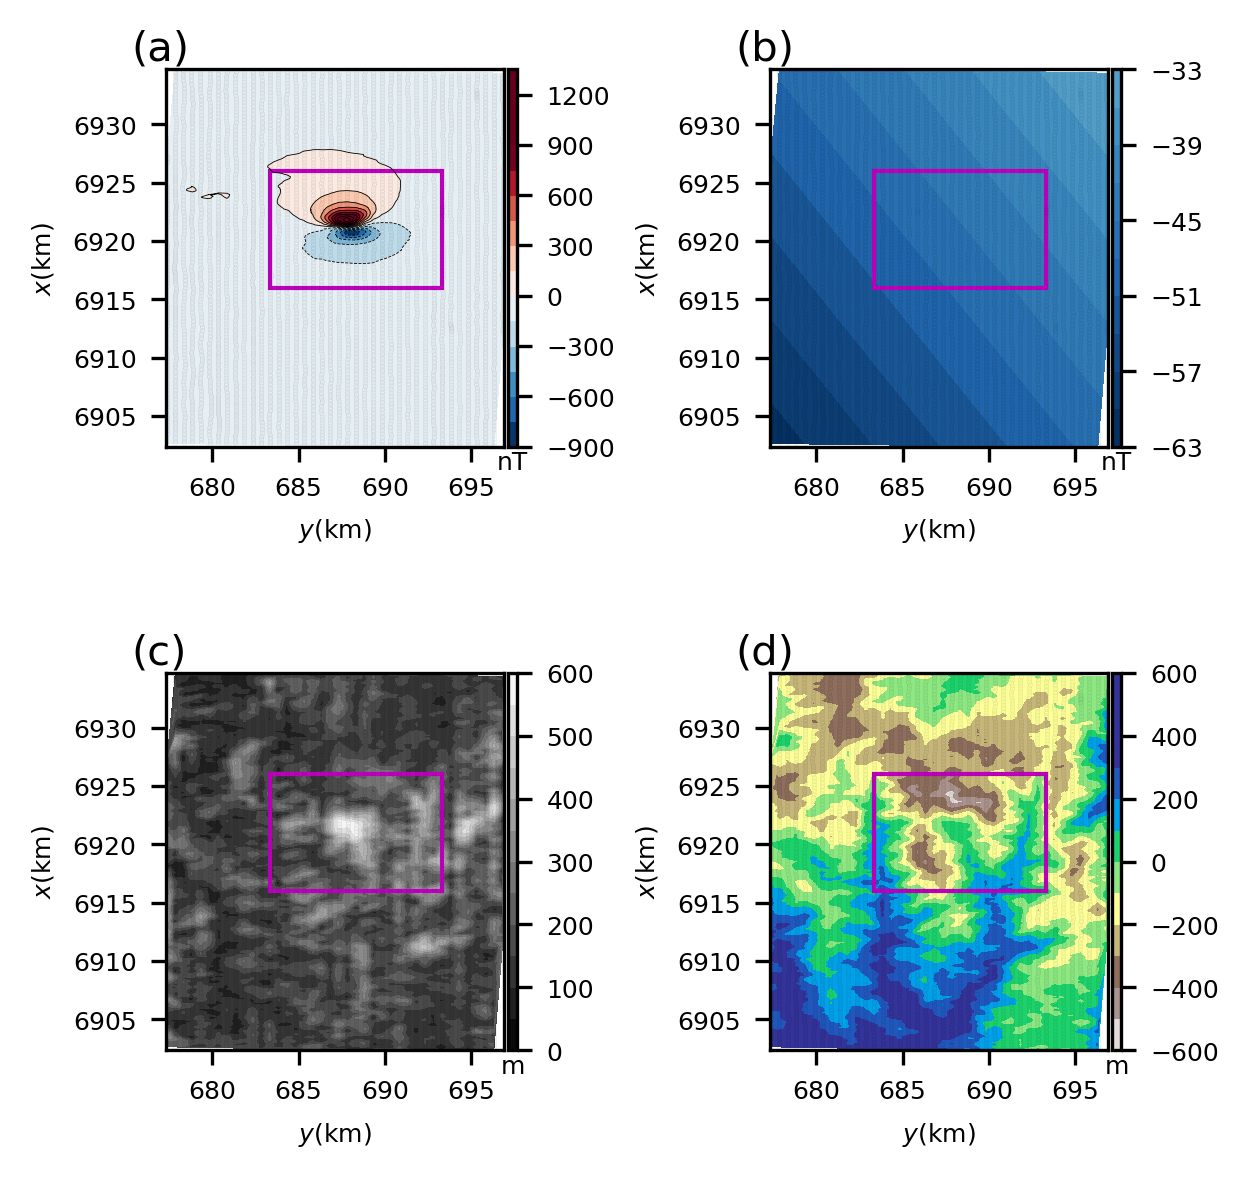
\includegraphics[width=\textwidth]{anitapolis_data.png}
	\caption{Aplicação aos dados do complexo de Anitápolis. 
		(a) Anomalia de campo total observada.
		(b) Polinômio de primeira ordem que representa o campo regional.
		(c) e (d) Altura geométrica dos pontos de observação e topografia,
		ambas referenciadas ao elipsoide WGS84. Por simplicidade, foi removida uma constante de $800$ m de seus valores. As coordenadas UTM estão referenciadas ao meridiano central $51^{\circ}$. Os pontos pretos representam os pontos observados. Apenas os dados delimitados pelo retângulo rosa foram usados para a inversão. 
	}
	\label{fig:anitapolis_data}
\end{figure}
\pagebreak
\begin{figure}[!htb]
	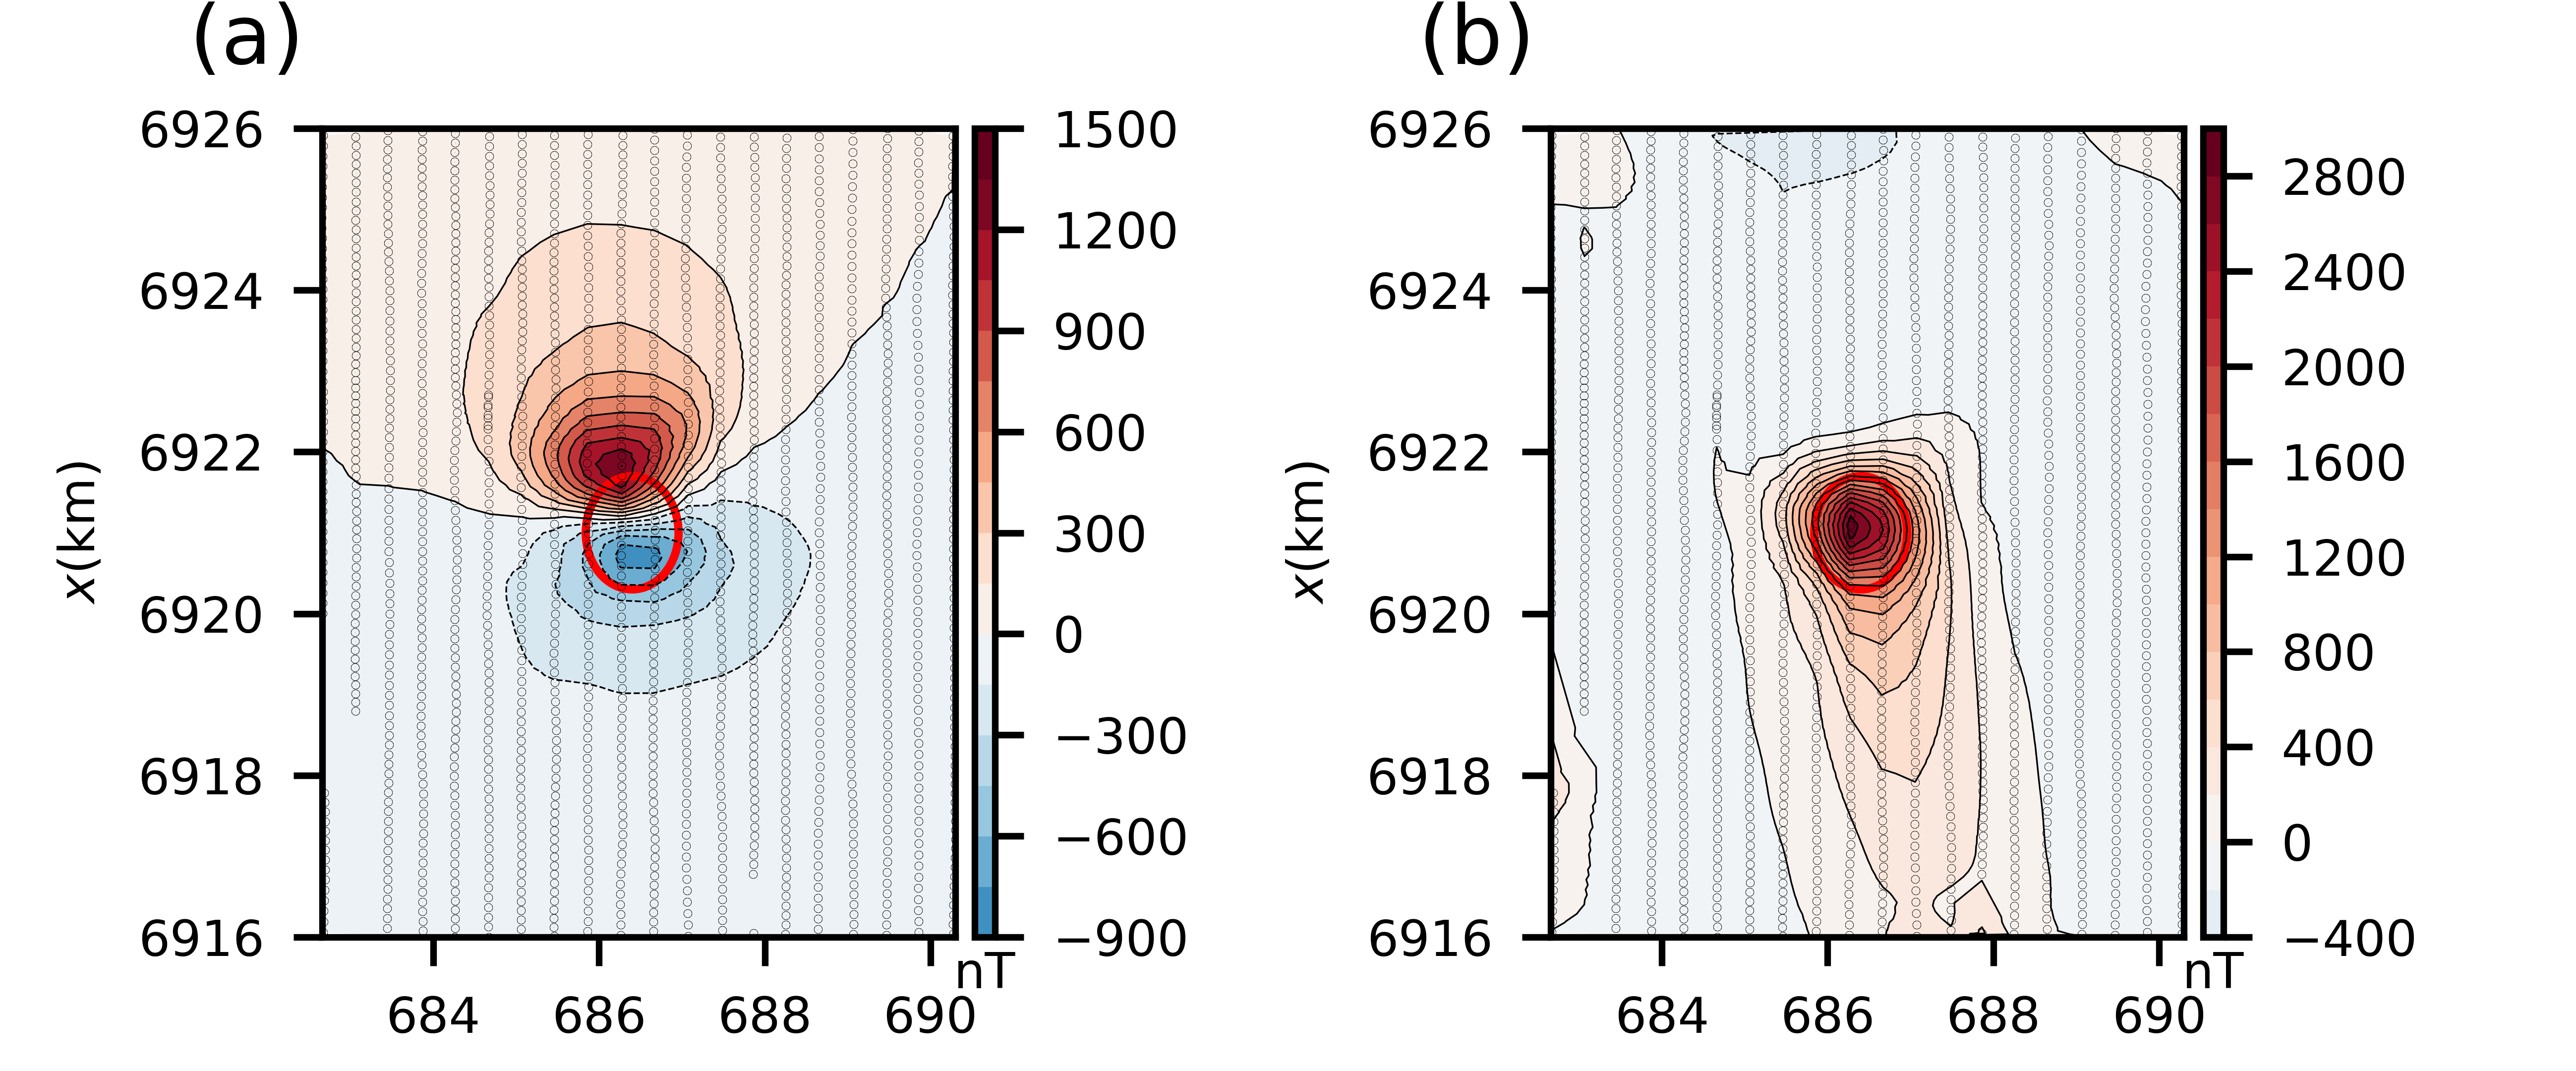
\includegraphics[width=\textwidth]{anitapolis_rtp.png}
	\caption{Aplicação aos dados do complexo de Anitápolis. 
		(a) e (b) Anomalias residual e RTP sobre a área de estudo definida pelo retângulo rosa na Figura \ref{fig:anitapolis_data}.
		A linha vermelha representa a projeção horizontal das aproximações iniciais usadas nas inversões subsequentes (prismas vermelhos nas Figuras 
		\ref{fig:anitapolis_l2_result}c e \ref{fig:anitapolis_l1_result}c).
	}
	\label{fig:anitapolis_rtp_residual}
\end{figure}

\pagebreak

\begin{figure}[!htb]
	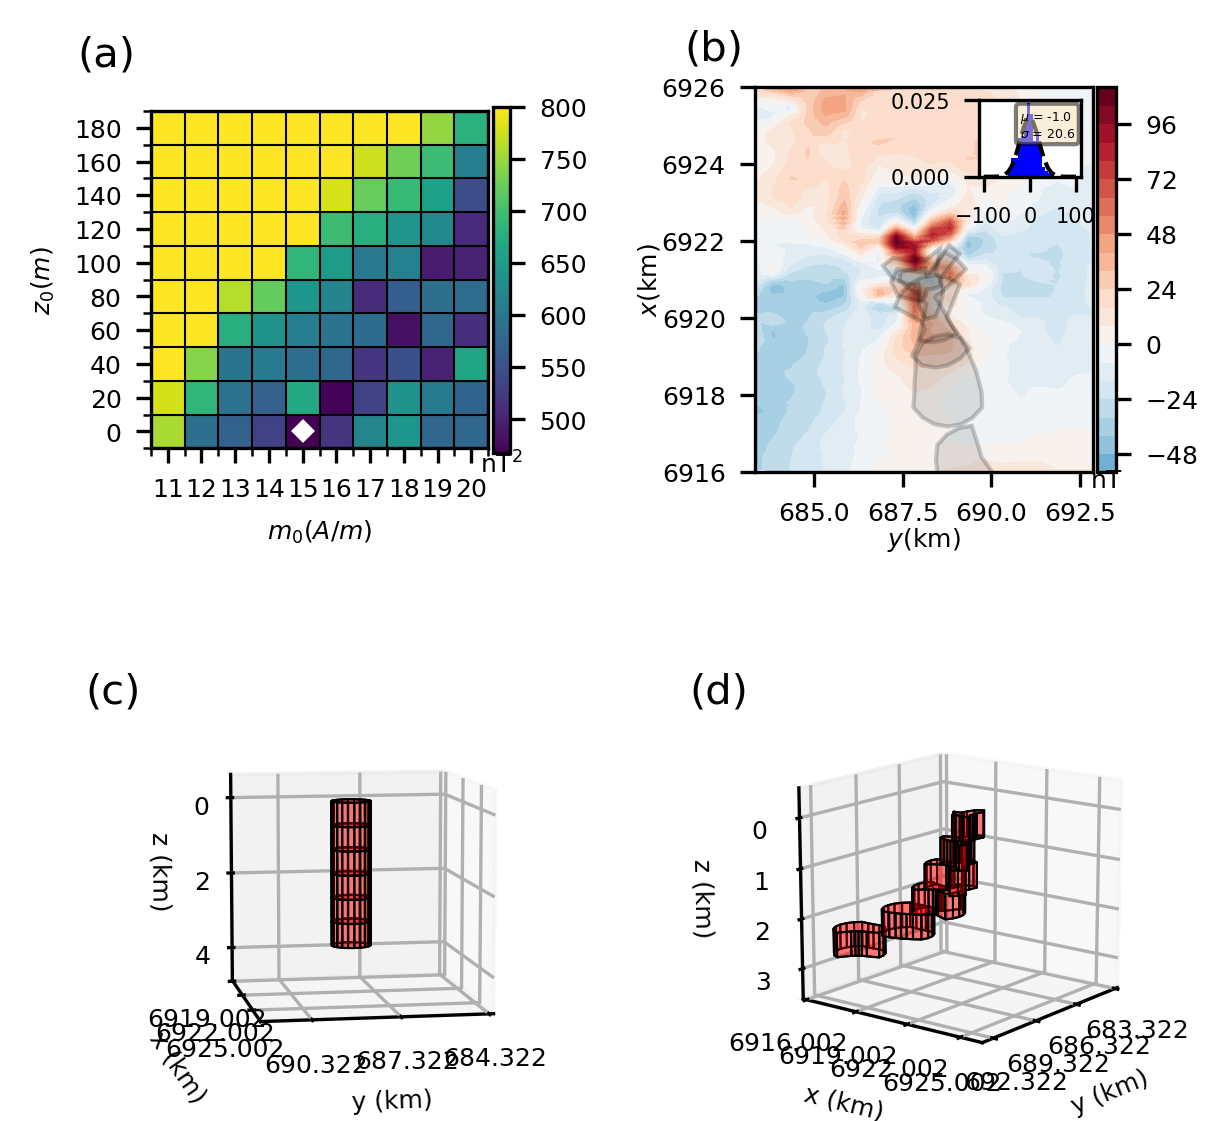
\includegraphics[width=\textwidth]{anitapolis-l2-solution.png}
	\caption{Soluções L2 obtidas para o complexo de Anitápolis. 
		(a) Mapa discreto da função objetivo produzida pelos modelos obtidos a partir da varredura de valores de profundidade do topo $z_{0}$ e intensidade de magnetização total $m_{0}$. 
		O losango branco representa os valores de $m_{0}$ e $z_{0})$ que definem a melhor solução L2.
		(b) Resíduos entre a anomalia de campo total residual (Fig. \ref{fig:anitapolis_rtp_residual}a) e os dados preditos (não exibidos) produzidos pela melhor solução L2 (prismas vermelhos no painel d). 
		O histograma dos resíduos inserido em (b) mostra a curva
		Gaussiana ajustada (linha tracejada). 
		(c) e (d) Visualizações em perspectiva da aproximação inicial e da melhor solução, respectivamente.
	}
	\label{fig:anitapolis_l2_result}
\end{figure}

\pagebreak

\begin{figure}[!htb]
	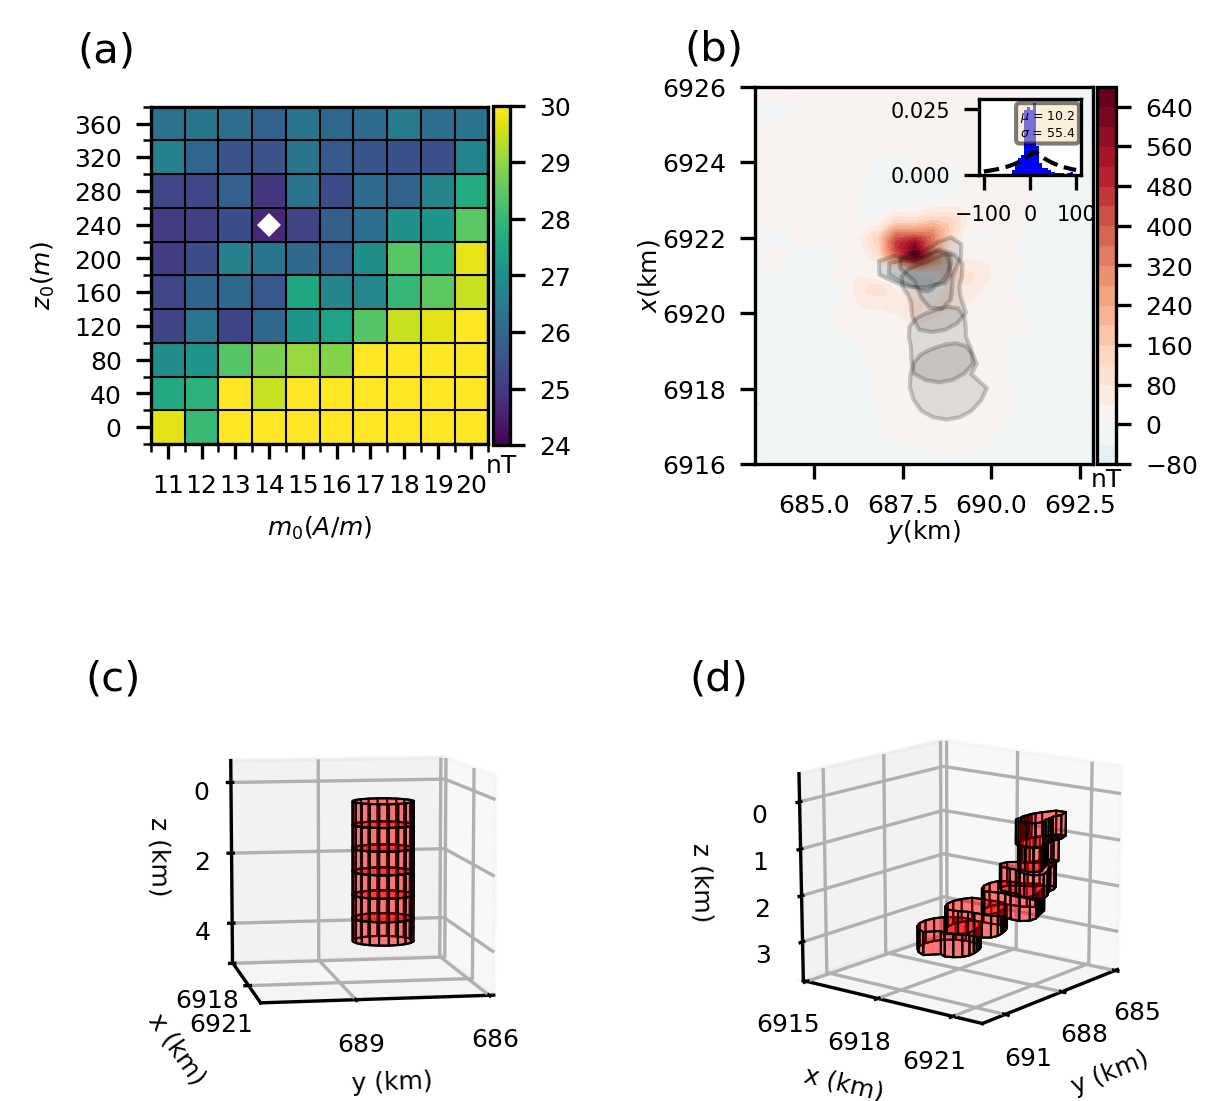
\includegraphics[width=\textwidth]{anitapolis-l1-solution.png}
	\caption{Soluções L1 obtidas para o complexo de Anitápolis. 
		(a) Mapa discreto da função objetivo produzida pelos modelos obtidos a partir da varredura de valores de profundidade do topo $z_{0}$ e intensidade de magnetização total $m_{0}$. 
		O losango branco representa os valores de $m_{0}$ e $z_{0})$ que definem a melhor solução L1.
		(b) Resíduos entre a anomalia de campo total residual (Fig. \ref{fig:anitapolis_rtp_residual}a) e os dados preditos (não exibidos) produzidos pela melhor solução L1 (prismas vermelhos no painel d). 
		O histograma dos resíduos inserido em (b) mostra a curva
		Laplaciana ajustada (linha tracejada). 
		(c) e (d) Visualizações em perspectiva da aproximação inicial e da melhor solução, respectivamente.
	}
	\label{fig:anitapolis_l1_result}
\end{figure}
\pagebreak


\section{Complexo de Diorama}
\label{subsec:diorama_complex}


A província alcalina de Goiás (PAGO) é resultado de um magmatismo máfico-alcalino que ocorreu no final do Cretáceo, na borda da Bacia do Paraná.
Ela é associada com uma grande variedade petrográfica que incluem complexos máficos e ultra-máficos, intrusões alcalinas subvulcânicas e vulcânicas que coincidem com uma bem definida tendência de falhas no embasamento de N30O \citep{junqueirabrod_etal2002, junqueira_brod2005}.
Diferentes estudos geofísicos indicam que as anomalias magnéticas associadas às intrusões alcalinas na PAGO são afetadas por notáveis magnetizações remanentes \citep[por exemplo,][]{dutra_etal2012, marangoni_mantovani2013, 
dutra_etal2014, oliveirajr_etal2015, zhang-2018, reis_etal2020}.

As Figuras \ref{fig:diorama_data}a e \ref{fig:diorama_data}b mostram, respectivamente, 
a anomalia de campo total observada e o campo regional estimado sobre o complexo de Diorama na parte norte da PAGO \citep{junqueira_brod2005,
marangoni_mantovani2013, oliveirajr_etal2015}.
O levantamento aéreo foi adquirido com linhas N-S e L-O espaçadas em $500$ m e $10,000$ m umas das outras, respectivamente, sobre a superfície ondulada mostrada na Figura 
\ref{fig:diorama_data}c. 
A Figura \ref{fig:diorama_data}d mostra a topografia na área de estudo.
A inclinação e a declinação do campo geomagnético principal na área de estudo, para a época da aquisição $(2004)$, são $-19.5^{\circ}$ e 
$-18.5^{\circ}$, respectivamente.

A Figura \ref{fig:diorama_rtp_residual}a mostra a anomalia de campo total residual obtida pela subtração do campo regional estimado (Fig. \ref{fig:diorama_data}b)
da anomalia de campo total observada (Fig. \ref{fig:diorama_data}a).
A partir dessa anomalia residual, foi calculada a anomalia RTP mostrada na Figura \ref{fig:diorama_rtp_residual}b utilizando a direção de magnetização estimada por \citet{zhang-2018} com inclinação $-46^{\circ}$ e declinação $24^{\circ}$.
A área positiva da anomalia RTP estimada foi usada para definir as aproximações iniciais para todas as soluções L2 (Fig. \ref{fig:diorama_l2_result}) e L1 
(Fig. \ref{fig:diorama_l1_result}) obtidas pelo método ao realizar a inversão da anomalia de campo total residual mostrada na Figura \ref{fig:diorama_rtp_residual}a.
Todas essas soluções L2 e L1 foram obtidas através da utilização do seguinte conjunto de pesos normalizados $\tilde{\alpha}_{\ell}$ (Equação \ref{eq:alphas}):
$\tilde{\alpha}_{1} = 10^{-4}$, $\tilde{\alpha}_{2} = 10^{-4}$, 
$\tilde{\alpha}_{3} = 10^{-4}$, $\tilde{\alpha}_{4} = 10^{-6}$, e
$\tilde{\alpha}_{5} = 10^{-6}$.

A Figura \ref{fig:diorama_l2_result}a mostra os valores da função objetivo produzidos pelas 100 soluções L2 obtidas por uma malha de varredura de $10 \times 10$ valores de profundidade do topo $z_{0}$ e intensidade de magnetização total $m_{0}$.
A melhor solução L2 possui uma profundidade do topo de $z_{0} = 200$ m, intensidade de magnetização total de $m_{0} = 19$ A/m e uma profundidade da base em $2128.6$ m.
A Figura \ref{fig:diorama_l1_result}a exibe os valores da função objetivo produzidos pelas 100 soluções L2 obtidas por uma malha de varredura de $10 \times 10$ valores de profundidade do topo $z_{0}$ e intensidade de magnetização total $m_{0}$.
A melhor solução L1 possui uma profundidade do topo de $z_{0} = 250$ m, intensidade de magnetização total de $m_{0} = 18$ A/m e uma profundidade da base em $2692.0$ m.

As intensidades de magnetização total das soluções estão ambas em acordo com as medidas de laboratório conduzidas por \citet{dutra2011} e \citet{dutra_etal2014} 
em amostras de rochas da PAGO. Eles Eles encontraram valores que variam de $\approx 0.01$ to $20$ A/m.
A extensão vertical total da melhor solução L2 ($1928.6$ m) é $\approx 500$ m 
menor que a extensão da melhor solução L1 ($2442.0$ m), o que é consistente com a intensidade de magnetização menor da solução L1.
A extensão vertical total da solução L1 ($2192.0$ m), entretanto, é significativamente menor do que a obtida por \citet[][Fig. 4.9, p. 78]{dutra2011} para o complexo de Diorama ($\approx 3000.0$ m). 
É importante enfatizar que \cite{dutra2011} obteve essa extensão vertical total indiretamente ao estimar a distribuição de susceptibilidade magnética em uma malha 3D pouco refinada de prismas retangulares justapostos com lado de $1$ km de comprimento e valores máximos de susceptibilidade limitados a $0.01$ SI.
Essa malha foi projetada para investigar não só o complexo de Diorama como também todas as anomalias produzidas por extensos complexos alcalinos na área de estudo. Como consequência, os resultados apresentados por
\citet{dutra2011}, também relatado por \citet{marangoni_mantovani2013}, pode não ter resolução espacial suficiente para representar o complexo de Diorama aparentemente menor que os complexos ao seu redor.
Essa falta de resolução espacial associada ao limite superior imposto à distribuição de susceptibilidade magnética pode acarretar em uma extensão vertical total exagerada obtida para o complexo de Diorama.
Comparado à abordagem utilizada por \citet{dutra2011}, o método apresentado neste trabalho é capaz de representar o complexo de Diorama com uma maior resolução espacial e, dessa maneira, pode ser a principal causa da estimativa discrepante da extensão vertical total.

A solução L2 mostra uma forma complexa que depende da profundidade com nenhum controle estrutural aparente. É possível notar que seu prisma mais profundo possui uma área maior que a dos prismas restantes. As características dessa solução assemelham-se com as da solução L2 obtida para o dado sintético com a presença de uma fonte não-alvo pequena (Fig. \ref{fig:small_l2_result}).
Por outro lado, a Figura \ref{fig:diorama_l1_result} mostra uma solução L1 com uma forma que varia continuamente ao longo da profundidade que parece ser influenciada por uma falha aproximadamente orientada a N50$ ^\circ $L. Essa direção concorda com a relatada por
\citet{junqueirabrod_etal2002} para dique que cruzam o embasamento Pré-cambriano na área de estudo.
Esses resultados sugerem a presença de fontes não-alvo rasas localizadas próximas ao topo do complexo de Diorama.


%% Application to Diorama data

\begin{figure}[!htb]
	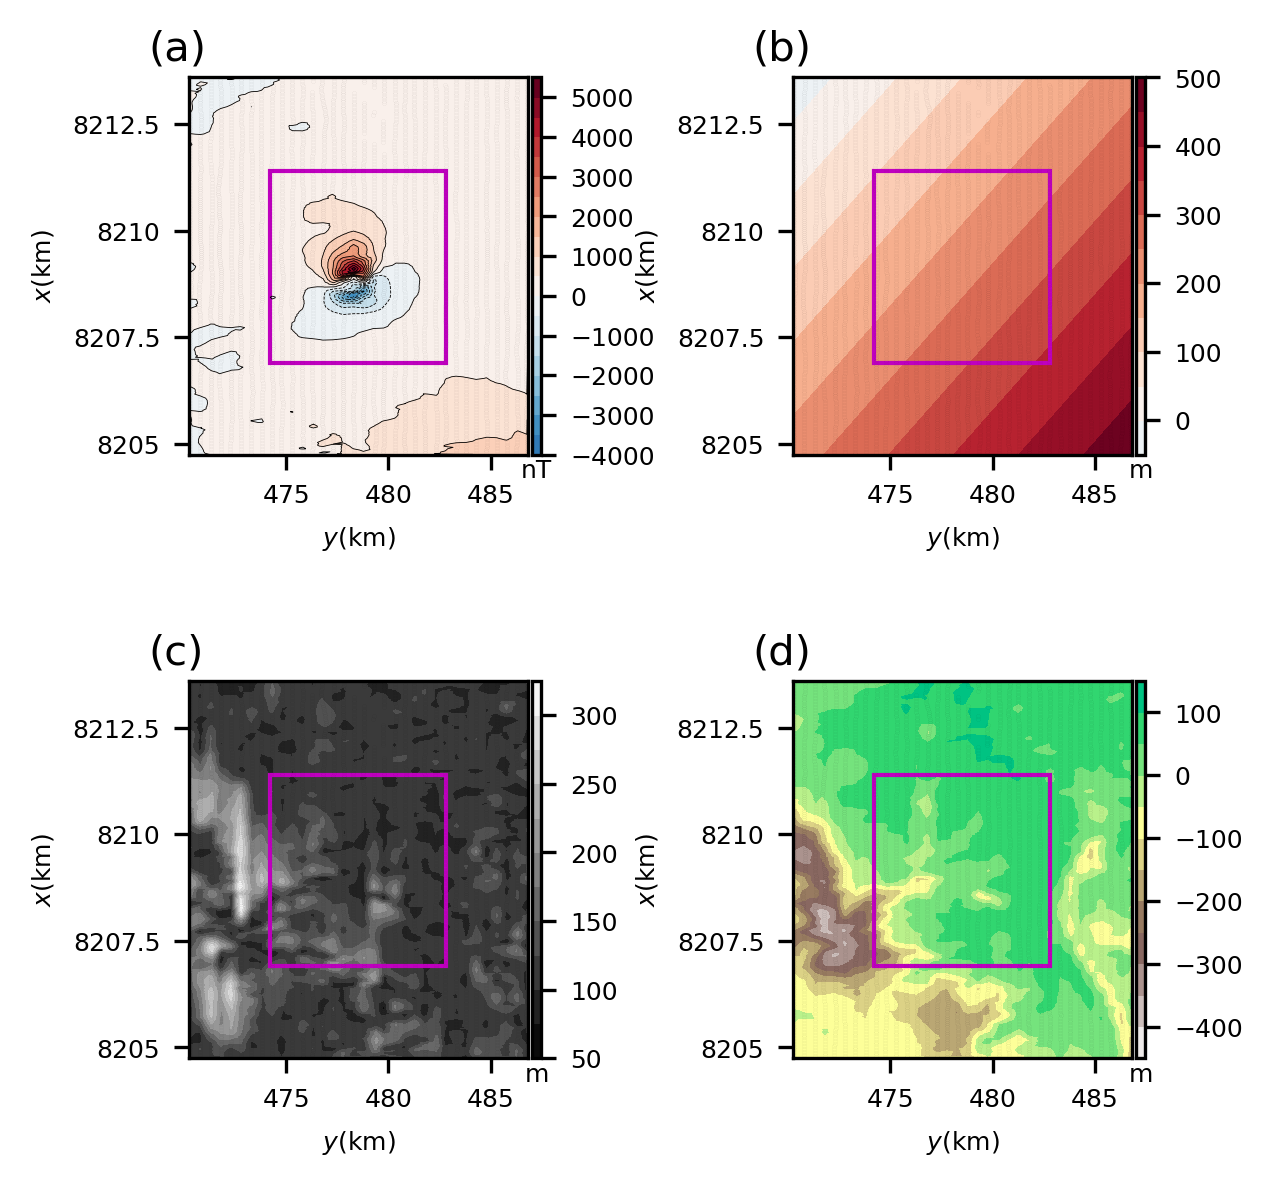
\includegraphics[width=\textwidth]{diorama_data.png}
	\caption{Aplicação aos dados do complexo de Diorama. 
		(a) Anomalia de campo total observada.
		(b) Polinômio de primeira ordem que representa o campo regional.
		(c) e (d) Altura geométrica dos pontos de observação e topografia,
		ambas referenciadas ao elipsoide WGS84. Por simplicidade, foi removida uma constante de $430$ m de seus valores. As coordenadas UTM estão referenciadas ao meridiano central $51^{\circ}$. Os pontos pretos representam os pontos observados. Apenas os dados delimitados pelo retângulo rosa foram usados para a inversão. 
	}
	\label{fig:diorama_data}
\end{figure}
\pagebreak

\begin{figure}[!htb]
	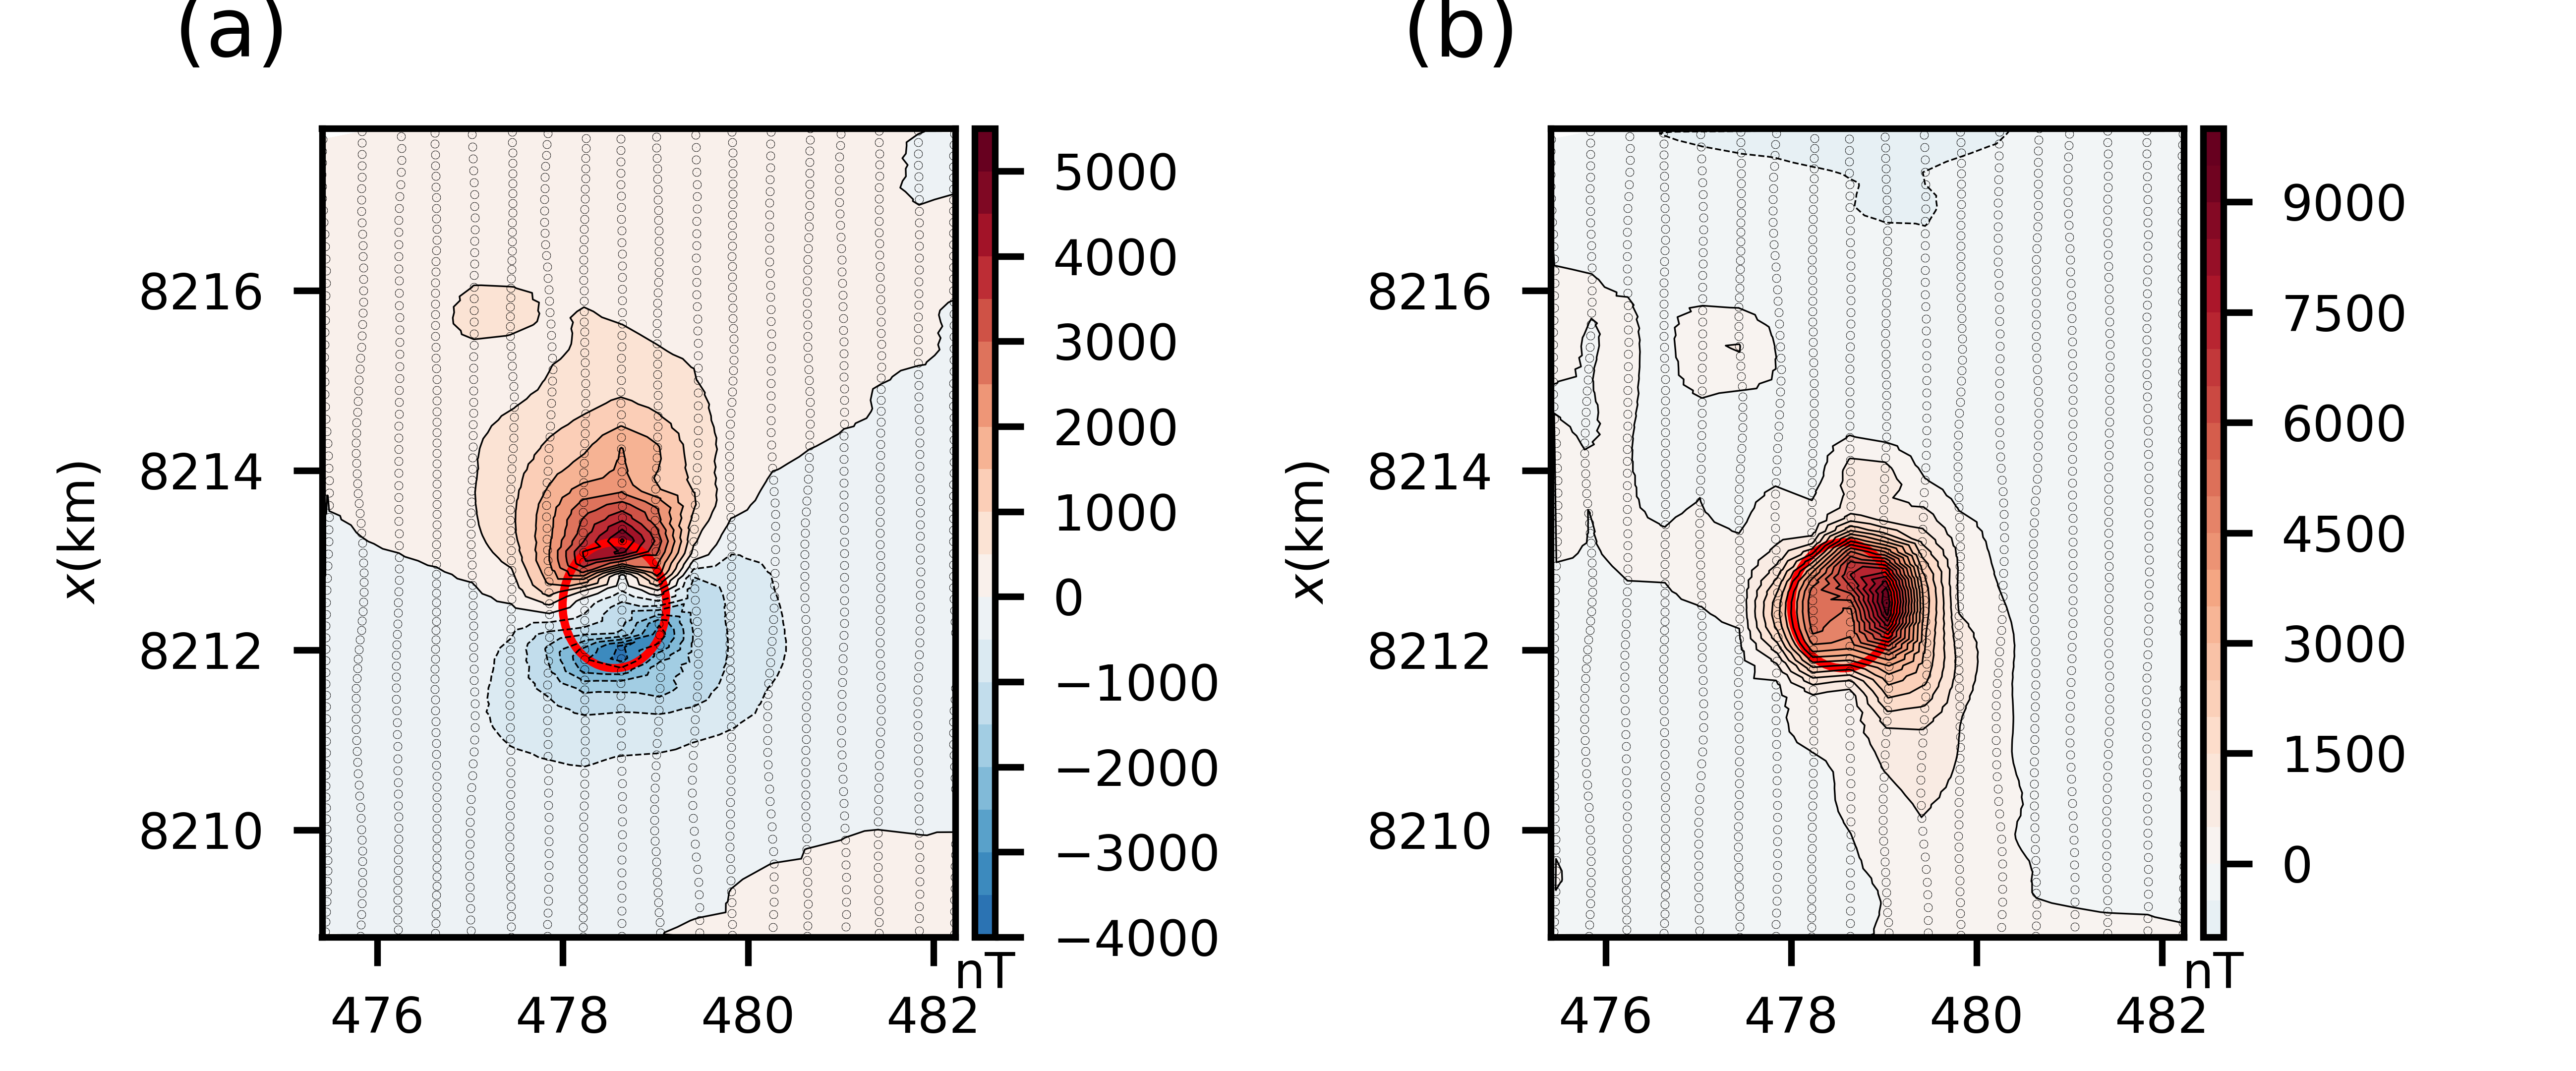
\includegraphics[width=\textwidth]{diorama_rtp.png}
	\caption{Aplicação aos dados do complexo de Diorama. 
		(a) e (b) Anomalias residual e RTP sobre a área de estudo definida pelo retângulo rosa na Figura \ref{fig:diorama_data}.
		A linha vermelha representa a projeção horizontal das aproximações iniciais usadas nas inversões subsequentes (prismas vermelhos nas Figuras \ref{fig:diorama_l2_result}c e \ref{fig:diorama_l1_result}c).
	}
	\label{fig:diorama_rtp_residual}
\end{figure}

\pagebreak
\begin{figure}[!htb]
	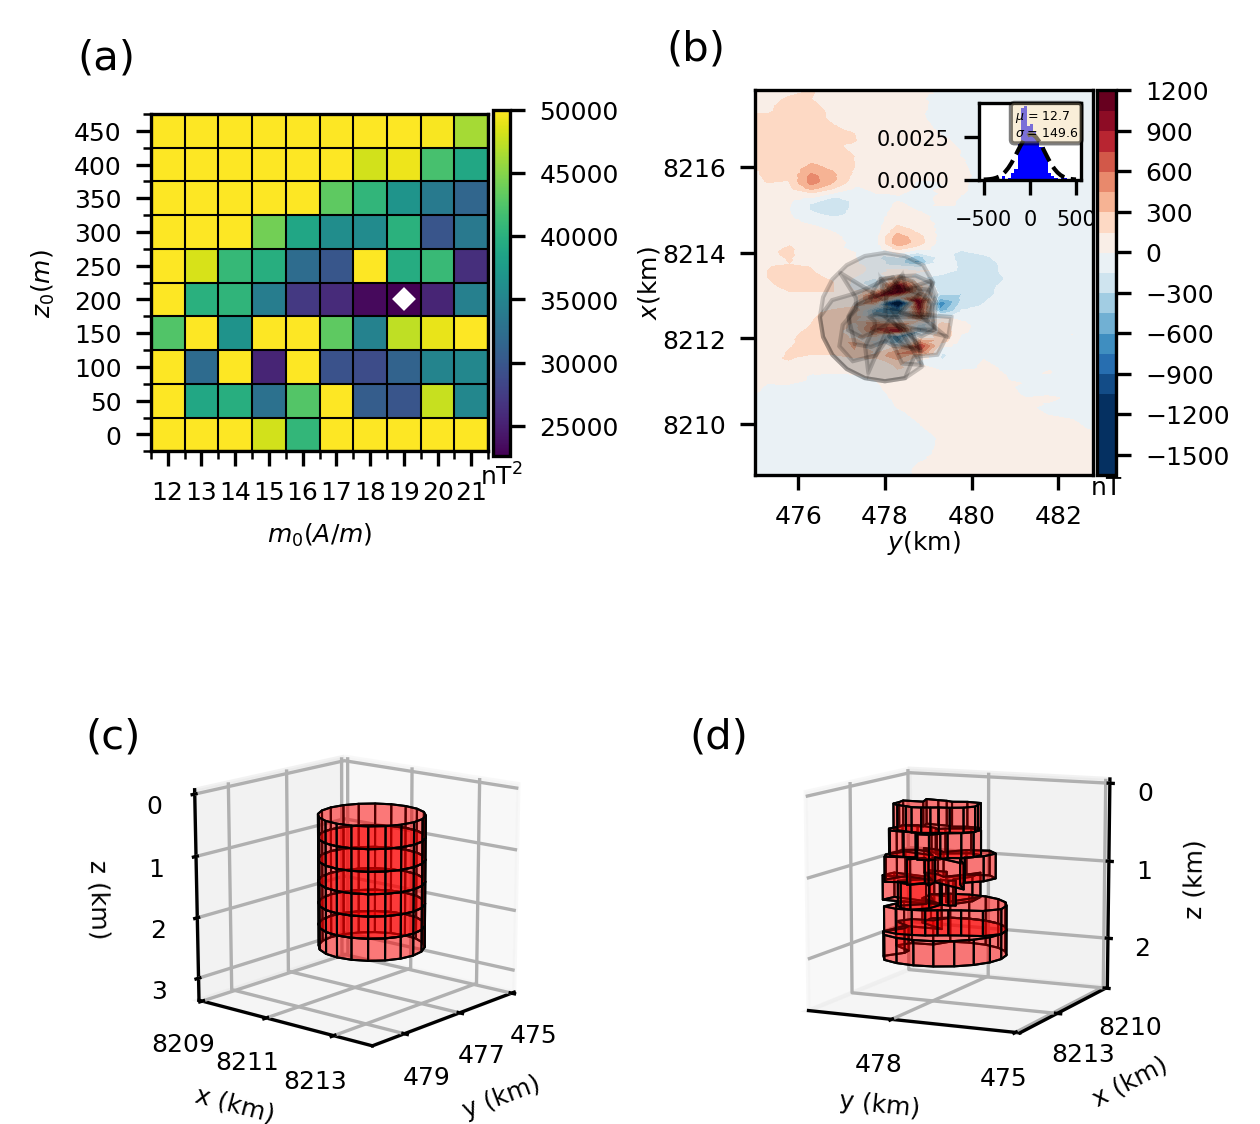
\includegraphics[width=\textwidth]{diorama-l2-solution.png}
	\caption{Soluções L2 obtidas para o complexo de Diorama. 
		(a) Mapa discreto da função objetivo produzida pelos modelos obtidos a partir da varredura de valores de profundidade do topo $z_{0}$ e intensidade de magnetização total $m_{0}$. 
		O losango branco representa os valores de $m_{0}$ e $z_{0})$ que definem a melhor solução L2.
		(b) Resíduos entre a anomalia de campo total residual (Fig. \ref{fig:diorama_rtp_residual}a) e os dados preditos (não exibidos) produzidos pela melhor solução L2 (prismas vermelhos no painel d). 
		O histograma dos resíduos inserido em (b) mostra a curva
		Gaussiana ajustada (linha tracejada). 
		(c) e (d) Visualizações em perspectiva da aproximação inicial e da melhor solução, respectivamente.
	}
	\label{fig:diorama_l2_result}
\end{figure}

\pagebreak
\begin{figure}[!htb]
	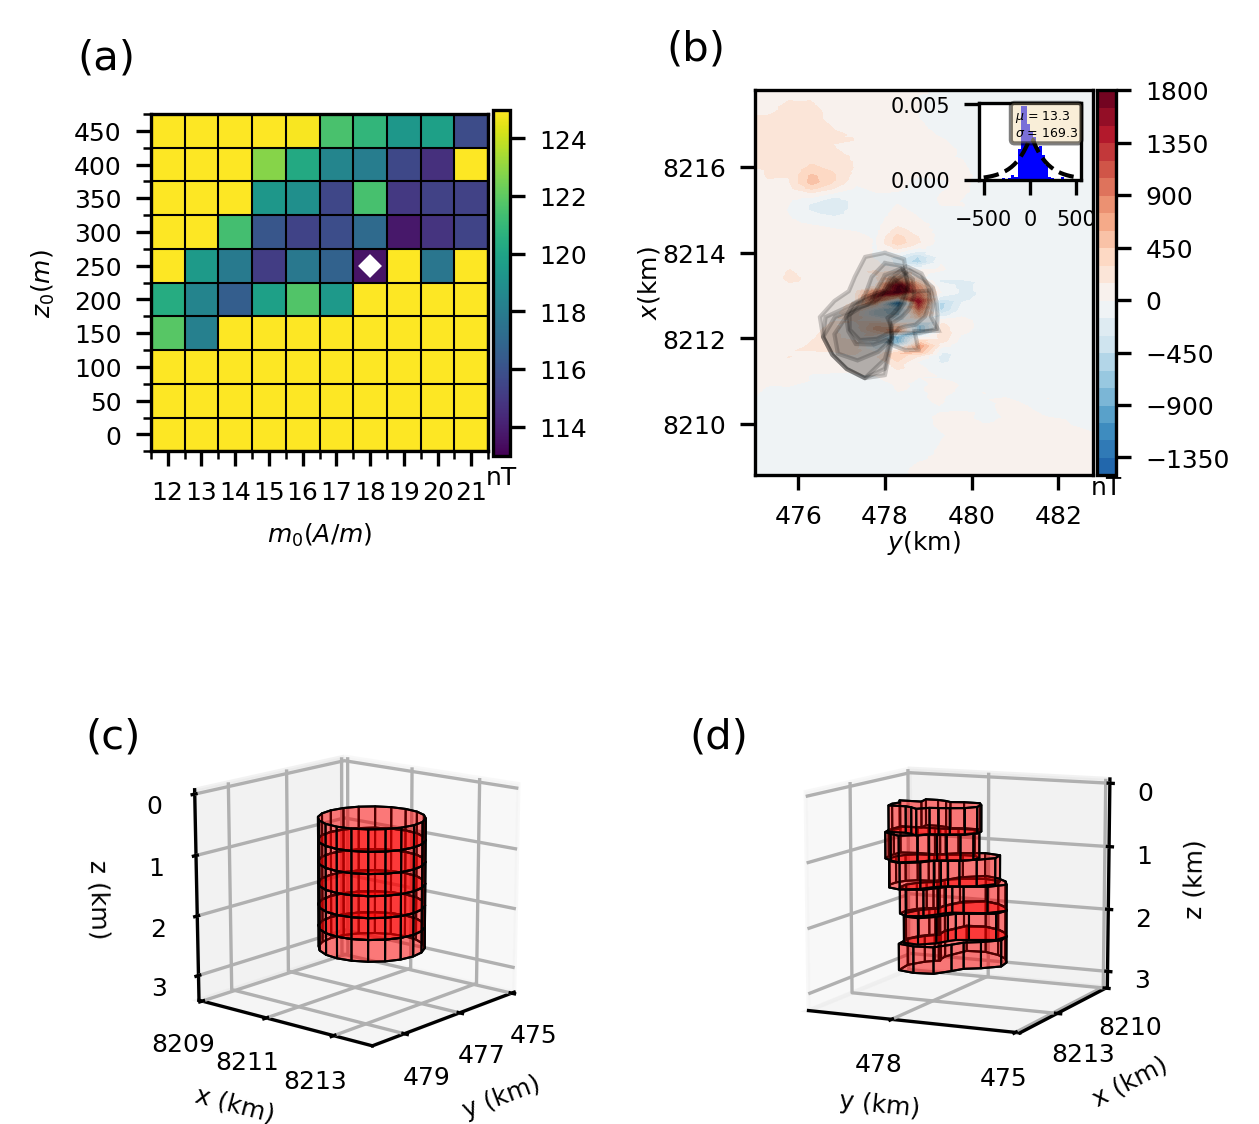
\includegraphics[width=\textwidth]{diorama-l1-solution.png}
	\caption{Soluções L1 obtidas para o complexo de Diorama. 
		(a) Mapa discreto da função objetivo produzida pelos modelos obtidos a partir da varredura de valores de profundidade do topo $z_{0}$ e intensidade de magnetização total $m_{0}$. 
		O losango branco representa os valores de $m_{0}$ e $z_{0})$ que definem a melhor solução L1.
		(b) Resíduos entre a anomalia de campo total residual (Fig. \ref{fig:diorama_rtp_residual}a) e os dados preditos (não exibidos) produzidos pela melhor solução L1 (prismas vermelhos no painel d). 
		O histograma dos resíduos inserido em (b) mostra a curva
		Laplaciana ajustada (linha tracejada). 
		(c) e (d) Visualizações em perspectiva da aproximação inicial e da melhor solução, respectivamente.
	}
	\label{fig:diorama_l1_result}
\end{figure}
  \chapter{Conclusões}

Este trabalho apresentou uma inversão magnética regularizada não linear com um ajuste robusto a fim de estimar a forma 3D de uma fonte definida pelo intérprete como alvo na presença ou não de fontes não-alvo.
Aqui, uma fonte alvo é definida como aquela que dá origem ao sinal geofísico mais forte ou com maior extensão horizontal, independentemente de ser um alvo geológico de alto valor econômico.
Essa inversão não requer a filtragem prévia do sinal produzido pelas fontes não-alvo para isolar o sinal da fonte alvo.
Isso é realizado por meio da minimização das funções dos vínculos definidas no espaço dos parâmetros e a função de desajuste de dados magnéticos definida no espaço dos dados como a norma-1 dos resíduos.
As soluções estimadas são estabilizadas por funções vínculo definidas pelas regularizações de Tikhonov de ordem zero e de primeira ordem.
A inversão magnética robusta assume que a direção de magnetização total da fonte alvo é conhecida, uniforme e estima: i) a intensidade de magnetização total, ii) as profundidades do topo e da base, iii) a posição e iv) a forma do corpo 3D em profundidade.
A solução regularizada obtida minimizando-se a norma-1 dos resíduos é chamada solução L1.
Para fins de comparação, o método também estima a solução L2 que minimiza as mesmas funções dos vínculos e a função de desajuste dos dados magnéticos definida pela norma-$2$ dos resíduos.

Testes em dados sintéticos mostram que, na presença de fontes não-alvo que produzem anomalias interferentes, a solução L1 mostra um melhor desempenho que a L2 não apenas na recuperação da geometria da fonte alvo, mas também na estimativa dos valores de profundidade do topo e de intensidade de magnetização.
Na ausência de dados magnéticos interferentes, as soluções L1 e L2 apresentam comportamentos semelhantes.

Aplicações a dados aeromagnéticos sobre os complexos alcalinos de Anitápolis, SC, e Diorama, GO, permitiram inferir detalhes sobre seus controles estruturais.
A semelhança entre as soluções L1 e L2 obtidas no complexo Anitápolis sugerem a presença de fontes não-alvo pequenas e rasas.
Ambas as soluções L1 e L2 mostram uma fonte alvo mergulhando para noroeste, com strike definido por um lineamento tectônico conhecido na área.
No caso do complexo alcalino de Diorama, em GO, a solução L1 mostra uma intrusão principal (fonte alvo) sub-vertical, que parece ser controlada por uma falha conhecida com tendência a nordeste.
A solução L2 obtida neste caso se mostrou muito diferente da L1,
o que sugere a presença
de ruído geológico
associado à presença
de fontes não-alvo
relativamente grandes.
Por conta disso, a solução L1 é considerada
a mais plausível.

Sem o conhecimento da direção uniforme de magnetização total da fonte alvo, o método proposto neste trabalho, não é capaz de gerar soluções coerentes com a geologia.
Outra limitação deste método é a definição da aproximação inicial, uma vez que ela depende do cálculo prévio da anomalia RTP, de um ajuste preliminar dos dados observados, além da escolha do número de prismas e vértices.
Considero que esses são pontos a serem explorados futuramente para o aprimoramento do método.
Além disso, um novo desafio seria generalizar o método para estimar múltiplas fontes simultaneamente.
Essa generalização pode ser acompanhada pela inversão conjunta de diversos dados, tais como dados magnéticos, de gravidade e de gradiometria da gravidade.

  \backmatter
  \markright{\MakeUppercase{Referências Bibliográficas}}

  % estilo de citações por ordem alfabética (defaut da classe ONTeX)
  \bibliographystyle{on-plain}
  \bibliography{ref}

  \appendix
  % A linha "\include" abaixo inclui um capítulo de apêndice.
  % Edite o arquivo "appenA.tex" de acordo com as suas necessidades.
  % É possível incluir outros capítulos de apêndice. Para tanto,
  % crie outros arquivos "appenX.tex", de acordo com as suas necessidades,
  % e inclua-os no documento utilizando "\include{appenX}".
  %\chapter{Algumas Demonstrações}

\section{First section}

Aqui devem entrar demonstrações mais longas, revisões de conceitos mais básicos
ou qualquer detalhe pertinente que não seja adequado para o corpo da
dissertação/tese.

\begin{equation}
\Gamma(x, y, z) = \int\limits_{-\infty}^{+\infty}\int\limits_{-\infty}^{+\infty}
p(x', y', z_{c}) \, \frac{\partial}{\partial z} \frac{1}{r} \: dx' \, dy'
\label{eq:apendice1}
\end{equation}

\section{Second section}

\lipsum[3-5]

\section{Third section}

\begin{table}[h]
	\caption[Cópia da tabela do capítulo 2]
	{Cópia da tabela do capítulo 2 para ilustrar numeração no apêndice}
	\label{tab:citation-copy}
	\centering
	{\footnotesize
		\begin{tabular}{|c|c|c|}
			\hline
			Tipo da Publica{\c c}\~ao & \verb|\citep| & \verb|\citet|\\
			\hline
			Livro & \citep{book-example} & \citet{book-example}\\
			Artigo & \citep{article-example} & \citet{article-example}\\
			Relat\'orio & \citep{techreport-example} & \citet{techreport-example}\\
			Relat\'orio & \citep{techreport-exampleIn} & \citet{techreport-exampleIn}\\
			Anais de Congresso & \citep{inproceedings-example} &
			\citet{inproceedings-example}\\
			S\'eries & \citep{incollection-example} & \citet{incollection-example}\\
			Em Livro & \citep{inbook-example} & \citet{inbook-example}\\
			Disserta{\c c}\~ao de mestrado & \citep{mastersthesis-example} &
			\citet{mastersthesis-example}\\
			Tese de doutorado & \citep{phdthesis-example} & \citet{phdthesis-example}\\
			\hline
	\end{tabular}}
\end{table}

\end{document} 